\documentclass[twoside]{book}

% Packages required by doxygen
\usepackage{fixltx2e}
\usepackage{calc}
\usepackage{doxygen}
\usepackage{graphicx}
\usepackage[utf8]{inputenc}
\usepackage{makeidx}
\usepackage{multicol}
\usepackage{multirow}
\PassOptionsToPackage{warn}{textcomp}
\usepackage{textcomp}
\usepackage[nointegrals]{wasysym}
\usepackage[table]{xcolor}

% Font selection
\usepackage[T1]{fontenc}
\usepackage{mathptmx}
\usepackage[scaled=.90]{helvet}
\usepackage{courier}
\usepackage{amssymb}
\usepackage{sectsty}
\renewcommand{\familydefault}{\sfdefault}
\allsectionsfont{%
  \fontseries{bc}\selectfont%
  \color{darkgray}%
}
\renewcommand{\DoxyLabelFont}{%
  \fontseries{bc}\selectfont%
  \color{darkgray}%
}
\newcommand{\+}{\discretionary{\mbox{\scriptsize$\hookleftarrow$}}{}{}}

% Page & text layout
\usepackage{geometry}
\geometry{%
  a4paper,%
  top=2.5cm,%
  bottom=2.5cm,%
  left=2.5cm,%
  right=2.5cm%
}
\tolerance=750
\hfuzz=15pt
\hbadness=750
\setlength{\emergencystretch}{15pt}
\setlength{\parindent}{0cm}
\setlength{\parskip}{0.2cm}
\makeatletter
\renewcommand{\paragraph}{%
  \@startsection{paragraph}{4}{0ex}{-1.0ex}{1.0ex}{%
    \normalfont\normalsize\bfseries\SS@parafont%
  }%
}
\renewcommand{\subparagraph}{%
  \@startsection{subparagraph}{5}{0ex}{-1.0ex}{1.0ex}{%
    \normalfont\normalsize\bfseries\SS@subparafont%
  }%
}
\makeatother

% Headers & footers
\usepackage{fancyhdr}
\pagestyle{fancyplain}
\fancyhead[LE]{\fancyplain{}{\bfseries\thepage}}
\fancyhead[CE]{\fancyplain{}{}}
\fancyhead[RE]{\fancyplain{}{\bfseries\leftmark}}
\fancyhead[LO]{\fancyplain{}{\bfseries\rightmark}}
\fancyhead[CO]{\fancyplain{}{}}
\fancyhead[RO]{\fancyplain{}{\bfseries\thepage}}
\fancyfoot[LE]{\fancyplain{}{}}
\fancyfoot[CE]{\fancyplain{}{}}
\fancyfoot[RE]{\fancyplain{}{\bfseries\scriptsize Generated on Wed Sep 10 2014 19\+:23\+:43 for My Project by Doxygen }}
\fancyfoot[LO]{\fancyplain{}{\bfseries\scriptsize Generated on Wed Sep 10 2014 19\+:23\+:43 for My Project by Doxygen }}
\fancyfoot[CO]{\fancyplain{}{}}
\fancyfoot[RO]{\fancyplain{}{}}
\renewcommand{\footrulewidth}{0.4pt}
\renewcommand{\chaptermark}[1]{%
  \markboth{#1}{}%
}
\renewcommand{\sectionmark}[1]{%
  \markright{\thesection\ #1}%
}

% Indices & bibliography
\usepackage{natbib}
\usepackage[titles]{tocloft}
\setcounter{tocdepth}{3}
\setcounter{secnumdepth}{5}
\makeindex

% Hyperlinks (required, but should be loaded last)
\usepackage{ifpdf}
\ifpdf
  \usepackage[pdftex,pagebackref=true]{hyperref}
\else
  \usepackage[ps2pdf,pagebackref=true]{hyperref}
\fi
\hypersetup{%
  colorlinks=true,%
  linkcolor=blue,%
  citecolor=blue,%
  unicode%
}

% Custom commands
\newcommand{\clearemptydoublepage}{%
  \newpage{\pagestyle{empty}\cleardoublepage}%
}


%===== C O N T E N T S =====

\begin{document}

% Titlepage & ToC
\hypersetup{pageanchor=false,
             bookmarks=true,
             bookmarksnumbered=true,
             pdfencoding=unicode
            }
\pagenumbering{roman}
\begin{titlepage}
\vspace*{7cm}
\begin{center}%
{\Large My Project }\\
\vspace*{1cm}
{\large Generated by Doxygen 1.8.8}\\
\vspace*{0.5cm}
{\small Wed Sep 10 2014 19:23:43}\\
\end{center}
\end{titlepage}
\clearemptydoublepage
\tableofcontents
\clearemptydoublepage
\pagenumbering{arabic}
\hypersetup{pageanchor=true}

%--- Begin generated contents ---
\chapter{Main Page}
\label{index}\hypertarget{index}{}This module is a part of Open Communication Thin-\/\+Block S\+D\+K. 
\chapter{Deprecated List}
\label{deprecated}
\hypertarget{deprecated}{}

\begin{DoxyRefList}
\item[\label{deprecated__deprecated000002}%
\hypertarget{deprecated__deprecated000002}{}%
Member \hyperlink{group__opt__filter_ga40b8b72ce87dcece9185a0911ec2c588}{C\+O\+A\+P\+\_\+\+O\+P\+T\+\_\+\+D\+E\+L\+T\+A} (opt)]\{ Use \hyperlink{group__opt__filter_gacec6795999a3ddaa56025a70abdc1d38}{coap\+\_\+opt\+\_\+delta()} instead. \}  
\item[\label{deprecated__deprecated000004}%
\hypertarget{deprecated__deprecated000004}{}%
Member \hyperlink{group__opt__filter_gad8982f51d2fb676d4b4be50487bb8590}{C\+O\+A\+P\+\_\+\+O\+P\+T\+\_\+\+L\+E\+N\+G\+T\+H} (opt)]\{ Use \hyperlink{group__opt__filter_ga5616c72178d923fb02db863c87ee249f}{coap\+\_\+opt\+\_\+length()} instead. \}  
\item[\label{deprecated__deprecated000003}%
\hypertarget{deprecated__deprecated000003}{}%
Member \hyperlink{group__opt__filter_ga2abe054935d45806d901a90ce5c4bd5d}{C\+O\+A\+P\+\_\+\+O\+P\+T\+\_\+\+S\+E\+T\+D\+E\+L\+T\+A} (opt, val)]\{ Use \hyperlink{group__opt__filter_ga8b601ead68a35f2bcca8c101b0b93c23}{coap\+\_\+opt\+\_\+encode()} instead. \}  
\item[\label{deprecated__deprecated000001}%
\hypertarget{deprecated__deprecated000001}{}%
Member \hyperlink{option_8h_a099224ae51d2b85fb4cbeb5f07ce52f7}{C\+O\+A\+P\+\_\+\+O\+P\+T\+\_\+\+S\+I\+Z\+E} (opt)]\{ Use \hyperlink{option_8h_a683c0121b4028a90f612809437aaa3d0}{coap\+\_\+opt\+\_\+size()} instead. \}  
\item[\label{deprecated__deprecated000005}%
\hypertarget{deprecated__deprecated000005}{}%
Member \hyperlink{group__opt__filter_gac4348d760bb312fdc2f108ee3e8303a4}{C\+O\+A\+P\+\_\+\+O\+P\+T\+\_\+\+V\+A\+L\+U\+E} (opt)]\{ Use \hyperlink{group__opt__filter_ga0f80e7bb12dca927fdf5829804c84b0e}{coap\+\_\+opt\+\_\+value()} instead. \} 
\end{DoxyRefList}
\chapter{Bug List}
\label{bug}
\hypertarget{bug}{}

\begin{DoxyRefList}
\item[\label{bug__bug000001}%
\hypertarget{bug__bug000001}{}%
Member \hyperlink{group__uri__parse_ga11af018953df7b74380791222cc115a5}{coap\+\_\+split\+\_\+query} (const unsigned char $\ast$s, size\+\_\+t length, unsigned char $\ast$buf, size\+\_\+t $\ast$buflen)]This function does not reserve additional space for delta $>$ 12. 
\end{DoxyRefList}
\chapter{Module Index}
\section{Modules}
Here is a list of all modules\+:\begin{DoxyCompactList}
\item \contentsline{section}{Asynchronous Messaging}{\pageref{group__coap__async}}{}
\item \contentsline{section}{Block Transfer}{\pageref{group__block}}{}
\item \contentsline{section}{Clock Handling}{\pageref{group__clock}}{}
\item \contentsline{section}{Option Filters}{\pageref{group__opt__filter}}{}
\item \contentsline{section}{Pseudo Random Numbers}{\pageref{group__prng}}{}
\item \contentsline{section}{Resource observation}{\pageref{group__observe}}{}
\item \contentsline{section}{U\+R\+I Parsing Functions}{\pageref{group__uri__parse}}{}
\item \contentsline{section}{Socket Interface}{\pageref{group__socket}}{}
\end{DoxyCompactList}

\chapter{Namespace Index}
\section{Namespace List}
Here is a list of all documented namespaces with brief descriptions\+:\begin{DoxyCompactList}
\item\contentsline{section}{\hyperlink{namespaceOC}{O\+C} \\*This file contains the declaration of classes and its members related to \hyperlink{classOC_1_1OCObject}{O\+C\+Object} }{\pageref{namespaceOC}}{}
\end{DoxyCompactList}

\chapter{Hierarchical Index}
\section{Class Hierarchy}
This inheritance list is sorted roughly, but not completely, alphabetically\+:\begin{DoxyCompactList}
\item \contentsline{section}{attr\+\_\+t}{\pageref{structattr__t}}{}
\item \contentsline{section}{Client\+C\+B}{\pageref{structClientCB}}{}
\item \contentsline{section}{coap\+\_\+async\+\_\+state\+\_\+t}{\pageref{structcoap__async__state__t}}{}
\item \contentsline{section}{coap\+\_\+attr\+\_\+t}{\pageref{structcoap__attr__t}}{}
\item \contentsline{section}{coap\+\_\+block\+\_\+t}{\pageref{structcoap__block__t}}{}
\item \contentsline{section}{coap\+\_\+context\+\_\+t}{\pageref{structcoap__context__t}}{}
\item \contentsline{section}{coap\+\_\+hdr\+\_\+t}{\pageref{structcoap__hdr__t}}{}
\item \contentsline{section}{coap\+\_\+linkedlistnode}{\pageref{structcoap__linkedlistnode}}{}
\item \contentsline{section}{coap\+\_\+mid\+\_\+cache\+\_\+t}{\pageref{structcoap__mid__cache__t}}{}
\item \contentsline{section}{coap\+\_\+opt\+\_\+iterator\+\_\+t}{\pageref{structcoap__opt__iterator__t}}{}
\item \contentsline{section}{coap\+\_\+option}{\pageref{structcoap__option}}{}
\item \contentsline{section}{coap\+\_\+option\+\_\+t}{\pageref{structcoap__option__t}}{}
\item \contentsline{section}{coap\+\_\+parse\+\_\+iterator\+\_\+t}{\pageref{structcoap__parse__iterator__t}}{}
\item \contentsline{section}{coap\+\_\+pdu\+\_\+t}{\pageref{structcoap__pdu__t}}{}
\item \contentsline{section}{coap\+\_\+queue\+\_\+t}{\pageref{structcoap__queue__t}}{}
\item \contentsline{section}{coap\+\_\+resource\+\_\+t}{\pageref{structcoap__resource__t}}{}
\item \contentsline{section}{coap\+\_\+subscription\+\_\+t}{\pageref{structcoap__subscription__t}}{}
\item \contentsline{section}{coap\+\_\+uri\+\_\+t}{\pageref{structcoap__uri__t}}{}
\item \contentsline{section}{Intel\+:\+:C\+C\+F\+L\+:\+:A\+P\+I\+:\+:Device\+Event}{\pageref{classIntel_1_1CCFL_1_1API_1_1DeviceEvent}}{}
\item \contentsline{section}{Intel\+:\+:C\+C\+F\+L\+:\+:A\+P\+I\+:\+:Device\+Event\+:\+:Device\+Event\+Info}{\pageref{structIntel_1_1CCFL_1_1API_1_1DeviceEvent_1_1DeviceEventInfo}}{}
\item enable\+\_\+shared\+\_\+from\+\_\+this\begin{DoxyCompactList}
\item \contentsline{section}{Intel\+:\+:C\+C\+F\+L\+:\+:A\+P\+I\+:\+:Model}{\pageref{classIntel_1_1CCFL_1_1API_1_1Model}}{}
\begin{DoxyCompactList}
\item \contentsline{section}{Intel\+:\+:C\+C\+F\+L\+:\+:A\+P\+I\+:\+:Model\+Impl}{\pageref{classIntel_1_1CCFL_1_1API_1_1ModelImpl}}{}
\end{DoxyCompactList}
\item \contentsline{section}{O\+C\+:\+:I\+Client\+Wrapper}{\pageref{classOC_1_1IClientWrapper}}{}
\begin{DoxyCompactList}
\item \contentsline{section}{O\+C\+:\+:In\+Proc\+Client\+Wrapper}{\pageref{classOC_1_1InProcClientWrapper}}{}
\item \contentsline{section}{O\+C\+:\+:Out\+Of\+Proc\+Client\+Wrapper}{\pageref{classOC_1_1OutOfProcClientWrapper}}{}
\end{DoxyCompactList}
\item \contentsline{section}{oc\+:\+:ub\+:\+:O\+C\+Model}{\pageref{classoc_1_1ub_1_1OCModel}}{}
\begin{DoxyCompactList}
\item \contentsline{section}{oc\+:\+:ub\+:\+:O\+C\+Model\+Impl}{\pageref{classoc_1_1ub_1_1OCModelImpl}}{}
\end{DoxyCompactList}
\end{DoxyCompactList}
\item exception\begin{DoxyCompactList}
\item \contentsline{section}{O\+C\+:\+:Initialize\+Exception}{\pageref{classOC_1_1InitializeException}}{}
\item \contentsline{section}{O\+C\+:\+:Resource\+Init\+Exception}{\pageref{classOC_1_1ResourceInitException}}{}
\end{DoxyCompactList}
\item \contentsline{section}{Function\+Struct}{\pageref{structFunctionStruct}}{}
\item \contentsline{section}{Intel\+:\+:C\+C\+F\+L\+:\+:A\+P\+I\+:\+:Get\+Devices\+Result}{\pageref{classIntel_1_1CCFL_1_1API_1_1GetDevicesResult}}{}
\item \contentsline{section}{O\+C\+:\+:I\+Server\+Wrapper}{\pageref{classOC_1_1IServerWrapper}}{}
\begin{DoxyCompactList}
\item \contentsline{section}{O\+C\+:\+:In\+Proc\+Server\+Wrapper}{\pageref{classOC_1_1InProcServerWrapper}}{}
\item \contentsline{section}{O\+C\+:\+:Out\+Of\+Proc\+Server\+Wrapper}{\pageref{classOC_1_1OutOfProcServerWrapper}}{}
\end{DoxyCompactList}
\item \contentsline{section}{O\+C\+:\+:I\+Wrapper\+Factory}{\pageref{classOC_1_1IWrapperFactory}}{}
\begin{DoxyCompactList}
\item \contentsline{section}{O\+C\+:\+:Wrapper\+Factory}{\pageref{classOC_1_1WrapperFactory}}{}
\end{DoxyCompactList}
\item \contentsline{section}{list}{\pageref{structlist}}{}
\item \contentsline{section}{remoting\+:\+:Lite\+Connection}{\pageref{classremoting_1_1LiteConnection}}{}
\item \contentsline{section}{remoting\+:\+:Lite\+Remoting}{\pageref{classremoting_1_1LiteRemoting}}{}
\item Lite\+Session\begin{DoxyCompactList}
\item \contentsline{section}{remoting\+:\+:Lite\+Session\+Impl}{\pageref{classremoting_1_1LiteSessionImpl}}{}
\end{DoxyCompactList}
\item Lite\+Target\+Device\begin{DoxyCompactList}
\item \contentsline{section}{remoting\+:\+:Lite\+Target\+Device\+Proxy}{\pageref{classremoting_1_1LiteTargetDeviceProxy}}{}
\end{DoxyCompactList}
\item \contentsline{section}{O\+C\+Callback\+Data}{\pageref{structOCCallbackData}}{}
\item \contentsline{section}{O\+C\+Client\+Response}{\pageref{structOCClientResponse}}{}
\item \contentsline{section}{O\+C\+Co\+A\+P\+Token}{\pageref{structOCCoAPToken}}{}
\item \contentsline{section}{O\+C\+Dev\+Addr}{\pageref{structOCDevAddr}}{}
\item \contentsline{section}{oc\+:\+:ub\+:\+:O\+C\+Discover\+Services\+Result}{\pageref{classoc_1_1ub_1_1OCDiscoverServicesResult}}{}
\item \contentsline{section}{O\+C\+Entity\+Handler\+Request}{\pageref{structOCEntityHandlerRequest}}{}
\item \contentsline{section}{O\+C\+:\+:O\+C\+Object}{\pageref{classOC_1_1OCObject}}{}
\item \contentsline{section}{O\+C\+:\+:O\+C\+Observer}{\pageref{classOC_1_1OCObserver}}{}
\item \contentsline{section}{O\+C\+Observe\+Req}{\pageref{structOCObserveReq}}{}
\item \contentsline{section}{O\+C\+:\+:O\+C\+Observer\+Handler}{\pageref{classOC_1_1OCObserverHandler}}{}
\begin{DoxyCompactList}
\item \contentsline{section}{O\+C\+:\+:My\+Observer\+Handler}{\pageref{classOC_1_1MyObserverHandler}}{}
\end{DoxyCompactList}
\item \contentsline{section}{O\+C\+:\+:O\+C\+Platform}{\pageref{classOC_1_1OCPlatform}}{}
\item \contentsline{section}{O\+C\+:\+:O\+C\+Platform\+Handler}{\pageref{classOC_1_1OCPlatformHandler}}{}
\item \contentsline{section}{O\+C\+Presence}{\pageref{structOCPresence}}{}
\item \contentsline{section}{O\+C\+:\+:O\+C\+Representation}{\pageref{classOC_1_1OCRepresentation}}{}
\item \contentsline{section}{O\+C\+Request}{\pageref{structOCRequest}}{}
\item \contentsline{section}{O\+C\+:\+:O\+C\+Resource}{\pageref{classOC_1_1OCResource}}{}
\item \contentsline{section}{O\+C\+:\+:O\+C\+Resource\+Handler}{\pageref{classOC_1_1OCResourceHandler}}{}
\begin{DoxyCompactList}
\item \contentsline{section}{My\+Resource\+Handler}{\pageref{classMyResourceHandler}}{}
\item \contentsline{section}{O\+C\+:\+:My\+Multi\+Resource\+Handler}{\pageref{classOC_1_1MyMultiResourceHandler}}{}
\end{DoxyCompactList}
\item \contentsline{section}{O\+C\+:\+:O\+C\+Resource\+Request}{\pageref{classOC_1_1OCResourceRequest}}{}
\item \contentsline{section}{O\+C\+:\+:O\+C\+Resource\+Response}{\pageref{classOC_1_1OCResourceResponse}}{}
\item \contentsline{section}{O\+C\+Response}{\pageref{structOCResponse}}{}
\item \contentsline{section}{O\+C\+:\+:O\+C\+Security\+Model}{\pageref{classOC_1_1OCSecurityModel}}{}
\item \contentsline{section}{O\+C\+:\+:Platform\+Config}{\pageref{structOC_1_1PlatformConfig}}{}
\item Protocol\begin{DoxyCompactList}
\item \contentsline{section}{Intel\+:\+:C\+C\+F\+L\+:\+:Protocols\+:\+:Mock\+Protocol}{\pageref{classIntel_1_1CCFL_1_1Protocols_1_1MockProtocol}}{}
\end{DoxyCompactList}
\item \contentsline{section}{resourceinterface\+\_\+t}{\pageref{structresourceinterface__t}}{}
\item \contentsline{section}{Resource\+Observer}{\pageref{structResourceObserver}}{}
\item \contentsline{section}{resourcetype\+\_\+t}{\pageref{structresourcetype__t}}{}
\item \contentsline{section}{rsrc\+\_\+t}{\pageref{structrsrc__t}}{}
\item runtime\+\_\+error\begin{DoxyCompactList}
\item \contentsline{section}{O\+C\+:\+:O\+C\+Exception}{\pageref{classOC_1_1OCException}}{}
\end{DoxyCompactList}
\item \contentsline{section}{str}{\pageref{structstr}}{}
\item \contentsline{section}{U\+T\+\_\+hash\+\_\+bucket}{\pageref{structUT__hash__bucket}}{}
\item \contentsline{section}{U\+T\+\_\+hash\+\_\+handle}{\pageref{structUT__hash__handle}}{}
\item \contentsline{section}{U\+T\+\_\+hash\+\_\+table}{\pageref{structUT__hash__table}}{}
\end{DoxyCompactList}

\chapter{Class Index}
\section{Class List}
Here are the classes, structs, unions and interfaces with brief descriptions\+:\begin{DoxyCompactList}
\item\contentsline{section}{\hyperlink{structattr__t}{attr\+\_\+t} }{\pageref{structattr__t}}{}
\item\contentsline{section}{\hyperlink{structClientCB}{Client\+C\+B} }{\pageref{structClientCB}}{}
\item\contentsline{section}{\hyperlink{structcoap__async__state__t}{coap\+\_\+async\+\_\+state\+\_\+t} }{\pageref{structcoap__async__state__t}}{}
\item\contentsline{section}{\hyperlink{structcoap__attr__t}{coap\+\_\+attr\+\_\+t} }{\pageref{structcoap__attr__t}}{}
\item\contentsline{section}{\hyperlink{structcoap__block__t}{coap\+\_\+block\+\_\+t} }{\pageref{structcoap__block__t}}{}
\item\contentsline{section}{\hyperlink{structcoap__context__t}{coap\+\_\+context\+\_\+t} }{\pageref{structcoap__context__t}}{}
\item\contentsline{section}{\hyperlink{structcoap__hdr__t}{coap\+\_\+hdr\+\_\+t} }{\pageref{structcoap__hdr__t}}{}
\item\contentsline{section}{\hyperlink{structcoap__linkedlistnode}{coap\+\_\+linkedlistnode} }{\pageref{structcoap__linkedlistnode}}{}
\item\contentsline{section}{\hyperlink{structcoap__mid__cache__t}{coap\+\_\+mid\+\_\+cache\+\_\+t} }{\pageref{structcoap__mid__cache__t}}{}
\item\contentsline{section}{\hyperlink{structcoap__opt__iterator__t}{coap\+\_\+opt\+\_\+iterator\+\_\+t} }{\pageref{structcoap__opt__iterator__t}}{}
\item\contentsline{section}{\hyperlink{structcoap__option}{coap\+\_\+option} }{\pageref{structcoap__option}}{}
\item\contentsline{section}{\hyperlink{structcoap__option__t}{coap\+\_\+option\+\_\+t} }{\pageref{structcoap__option__t}}{}
\item\contentsline{section}{\hyperlink{structcoap__parse__iterator__t}{coap\+\_\+parse\+\_\+iterator\+\_\+t} }{\pageref{structcoap__parse__iterator__t}}{}
\item\contentsline{section}{\hyperlink{structcoap__pdu__t}{coap\+\_\+pdu\+\_\+t} }{\pageref{structcoap__pdu__t}}{}
\item\contentsline{section}{\hyperlink{structcoap__queue__t}{coap\+\_\+queue\+\_\+t} }{\pageref{structcoap__queue__t}}{}
\item\contentsline{section}{\hyperlink{structcoap__resource__t}{coap\+\_\+resource\+\_\+t} }{\pageref{structcoap__resource__t}}{}
\item\contentsline{section}{\hyperlink{structcoap__subscription__t}{coap\+\_\+subscription\+\_\+t} }{\pageref{structcoap__subscription__t}}{}
\item\contentsline{section}{\hyperlink{structcoap__uri__t}{coap\+\_\+uri\+\_\+t} }{\pageref{structcoap__uri__t}}{}
\item\contentsline{section}{\hyperlink{classIntel_1_1CCFL_1_1API_1_1DeviceEvent}{Intel\+::\+C\+C\+F\+L\+::\+A\+P\+I\+::\+Device\+Event} }{\pageref{classIntel_1_1CCFL_1_1API_1_1DeviceEvent}}{}
\item\contentsline{section}{\hyperlink{structIntel_1_1CCFL_1_1API_1_1DeviceEvent_1_1DeviceEventInfo}{Intel\+::\+C\+C\+F\+L\+::\+A\+P\+I\+::\+Device\+Event\+::\+Device\+Event\+Info} }{\pageref{structIntel_1_1CCFL_1_1API_1_1DeviceEvent_1_1DeviceEventInfo}}{}
\item\contentsline{section}{\hyperlink{structFunctionStruct}{Function\+Struct} }{\pageref{structFunctionStruct}}{}
\item\contentsline{section}{\hyperlink{classIntel_1_1CCFL_1_1API_1_1GetDevicesResult}{Intel\+::\+C\+C\+F\+L\+::\+A\+P\+I\+::\+Get\+Devices\+Result} }{\pageref{classIntel_1_1CCFL_1_1API_1_1GetDevicesResult}}{}
\item\contentsline{section}{\hyperlink{classOC_1_1IClientWrapper}{O\+C\+::\+I\+Client\+Wrapper} }{\pageref{classOC_1_1IClientWrapper}}{}
\item\contentsline{section}{\hyperlink{classOC_1_1InitializeException}{O\+C\+::\+Initialize\+Exception} }{\pageref{classOC_1_1InitializeException}}{}
\item\contentsline{section}{\hyperlink{classOC_1_1InProcClientWrapper}{O\+C\+::\+In\+Proc\+Client\+Wrapper} }{\pageref{classOC_1_1InProcClientWrapper}}{}
\item\contentsline{section}{\hyperlink{classOC_1_1InProcServerWrapper}{O\+C\+::\+In\+Proc\+Server\+Wrapper} }{\pageref{classOC_1_1InProcServerWrapper}}{}
\item\contentsline{section}{\hyperlink{classOC_1_1IServerWrapper}{O\+C\+::\+I\+Server\+Wrapper} }{\pageref{classOC_1_1IServerWrapper}}{}
\item\contentsline{section}{\hyperlink{classOC_1_1IWrapperFactory}{O\+C\+::\+I\+Wrapper\+Factory} }{\pageref{classOC_1_1IWrapperFactory}}{}
\item\contentsline{section}{\hyperlink{structlist}{list} }{\pageref{structlist}}{}
\item\contentsline{section}{\hyperlink{classremoting_1_1LiteConnection}{remoting\+::\+Lite\+Connection} }{\pageref{classremoting_1_1LiteConnection}}{}
\item\contentsline{section}{\hyperlink{classremoting_1_1LiteRemoting}{remoting\+::\+Lite\+Remoting} }{\pageref{classremoting_1_1LiteRemoting}}{}
\item\contentsline{section}{\hyperlink{classremoting_1_1LiteSessionImpl}{remoting\+::\+Lite\+Session\+Impl} }{\pageref{classremoting_1_1LiteSessionImpl}}{}
\item\contentsline{section}{\hyperlink{classremoting_1_1LiteTargetDeviceProxy}{remoting\+::\+Lite\+Target\+Device\+Proxy} }{\pageref{classremoting_1_1LiteTargetDeviceProxy}}{}
\item\contentsline{section}{\hyperlink{classIntel_1_1CCFL_1_1Protocols_1_1MockProtocol}{Intel\+::\+C\+C\+F\+L\+::\+Protocols\+::\+Mock\+Protocol} }{\pageref{classIntel_1_1CCFL_1_1Protocols_1_1MockProtocol}}{}
\item\contentsline{section}{\hyperlink{classIntel_1_1CCFL_1_1API_1_1Model}{Intel\+::\+C\+C\+F\+L\+::\+A\+P\+I\+::\+Model} }{\pageref{classIntel_1_1CCFL_1_1API_1_1Model}}{}
\item\contentsline{section}{\hyperlink{classIntel_1_1CCFL_1_1API_1_1ModelImpl}{Intel\+::\+C\+C\+F\+L\+::\+A\+P\+I\+::\+Model\+Impl} }{\pageref{classIntel_1_1CCFL_1_1API_1_1ModelImpl}}{}
\item\contentsline{section}{\hyperlink{classOC_1_1MyMultiResourceHandler}{O\+C\+::\+My\+Multi\+Resource\+Handler} }{\pageref{classOC_1_1MyMultiResourceHandler}}{}
\item\contentsline{section}{\hyperlink{classOC_1_1MyObserverHandler}{O\+C\+::\+My\+Observer\+Handler} }{\pageref{classOC_1_1MyObserverHandler}}{}
\item\contentsline{section}{\hyperlink{classMyResourceHandler}{My\+Resource\+Handler} }{\pageref{classMyResourceHandler}}{}
\item\contentsline{section}{\hyperlink{structOCCallbackData}{O\+C\+Callback\+Data} }{\pageref{structOCCallbackData}}{}
\item\contentsline{section}{\hyperlink{structOCClientResponse}{O\+C\+Client\+Response} }{\pageref{structOCClientResponse}}{}
\item\contentsline{section}{\hyperlink{structOCCoAPToken}{O\+C\+Co\+A\+P\+Token} }{\pageref{structOCCoAPToken}}{}
\item\contentsline{section}{\hyperlink{structOCDevAddr}{O\+C\+Dev\+Addr} }{\pageref{structOCDevAddr}}{}
\item\contentsline{section}{\hyperlink{classoc_1_1ub_1_1OCDiscoverServicesResult}{oc\+::ub\+::\+O\+C\+Discover\+Services\+Result} }{\pageref{classoc_1_1ub_1_1OCDiscoverServicesResult}}{}
\item\contentsline{section}{\hyperlink{structOCEntityHandlerRequest}{O\+C\+Entity\+Handler\+Request} \\*The O\+C\+Entity\+Handler callback A\+P\+I must be implemented in the application in order to receive these requests }{\pageref{structOCEntityHandlerRequest}}{}
\item\contentsline{section}{\hyperlink{classOC_1_1OCException}{O\+C\+::\+O\+C\+Exception} }{\pageref{classOC_1_1OCException}}{}
\item\contentsline{section}{\hyperlink{classoc_1_1ub_1_1OCModel}{oc\+::ub\+::\+O\+C\+Model} }{\pageref{classoc_1_1ub_1_1OCModel}}{}
\item\contentsline{section}{\hyperlink{classoc_1_1ub_1_1OCModelImpl}{oc\+::ub\+::\+O\+C\+Model\+Impl} }{\pageref{classoc_1_1ub_1_1OCModelImpl}}{}
\item\contentsline{section}{\hyperlink{classOC_1_1OCObject}{O\+C\+::\+O\+C\+Object} \\*The \hyperlink{classOC_1_1OCObject}{O\+C\+Object} is the root abstract class from which many of the \hyperlink{namespaceOC}{O\+C} related objects derive from. It implements a common set of functionality supported by all the \hyperlink{namespaceOC}{O\+C} classes in the S\+D\+K such as object naming, I\+D, natural sort order and comparison }{\pageref{classOC_1_1OCObject}}{}
\item\contentsline{section}{\hyperlink{classOC_1_1OCObserver}{O\+C\+::\+O\+C\+Observer} }{\pageref{classOC_1_1OCObserver}}{}
\item\contentsline{section}{\hyperlink{structOCObserveReq}{O\+C\+Observe\+Req} }{\pageref{structOCObserveReq}}{}
\item\contentsline{section}{\hyperlink{classOC_1_1OCObserverHandler}{O\+C\+::\+O\+C\+Observer\+Handler} \\*\hyperlink{classOC_1_1OCObserverHandler}{O\+C\+Observer\+Handler} is a pure abstract class and it can be used for observer related callbacks }{\pageref{classOC_1_1OCObserverHandler}}{}
\item\contentsline{section}{\hyperlink{classOC_1_1OCPlatform}{O\+C\+::\+O\+C\+Platform} \\*Both server and client must initialize the core platform by instantiating \hyperlink{classOC_1_1OCPlatform}{O\+C\+Platform}. On successful initialization, an instance of the \hyperlink{classOC_1_1OCPlatform}{O\+C\+Platform} is returned. A\+P\+Is in \hyperlink{classOC_1_1OCPlatform}{O\+C\+Platform} provide mechanism to register a resource and host the resource on the server, find resources on the network etc }{\pageref{classOC_1_1OCPlatform}}{}
\item\contentsline{section}{\hyperlink{classOC_1_1OCPlatformHandler}{O\+C\+::\+O\+C\+Platform\+Handler} \\*\hyperlink{classOC_1_1OCPlatformHandler}{O\+C\+Platform\+Handler} is a pure abstract class and it can be used for registering and getting callbacks }{\pageref{classOC_1_1OCPlatformHandler}}{}
\item\contentsline{section}{\hyperlink{structOCPresence}{O\+C\+Presence} }{\pageref{structOCPresence}}{}
\item\contentsline{section}{\hyperlink{classOC_1_1OCRepresentation}{O\+C\+::\+O\+C\+Representation} }{\pageref{classOC_1_1OCRepresentation}}{}
\item\contentsline{section}{\hyperlink{structOCRequest}{O\+C\+Request} }{\pageref{structOCRequest}}{}
\item\contentsline{section}{\hyperlink{classOC_1_1OCResource}{O\+C\+::\+O\+C\+Resource} \\*\hyperlink{classOC_1_1OCResource}{O\+C\+Resource} represents an \hyperlink{namespaceOC}{O\+C} resource. A resource could be a light controller, temperature sensor, smoke detector, etc. A resource comes with a well-\/defined contract or interface onto which you can perform different operations, such as turning on the light, getting the current temperature or subscribing for event notifications from the smoke detector. A resource can be composed of one or more resources }{\pageref{classOC_1_1OCResource}}{}
\item\contentsline{section}{\hyperlink{classOC_1_1OCResourceHandler}{O\+C\+::\+O\+C\+Resource\+Handler} \\*\hyperlink{classOC_1_1OCResourceHandler}{O\+C\+Resource\+Handler} is a pure abstract class and it can be used for resource related callbacks }{\pageref{classOC_1_1OCResourceHandler}}{}
\item\contentsline{section}{\hyperlink{classOC_1_1OCResourceRequest}{O\+C\+::\+O\+C\+Resource\+Request} \\*\hyperlink{classOC_1_1OCResourceRequest}{O\+C\+Resource\+Request} provides A\+P\+Is to extract details from a request U\+R\+I }{\pageref{classOC_1_1OCResourceRequest}}{}
\item\contentsline{section}{\hyperlink{classOC_1_1OCResourceResponse}{O\+C\+::\+O\+C\+Resource\+Response} \\*\hyperlink{classOC_1_1OCResourceResponse}{O\+C\+Resource\+Response} provides A\+P\+Is to set the response details }{\pageref{classOC_1_1OCResourceResponse}}{}
\item\contentsline{section}{\hyperlink{structOCResponse}{O\+C\+Response} }{\pageref{structOCResponse}}{}
\item\contentsline{section}{\hyperlink{classOC_1_1OCSecurityModel}{O\+C\+::\+O\+C\+Security\+Model} \\*This class provides the required security model to access a service or a particular resource }{\pageref{classOC_1_1OCSecurityModel}}{}
\item\contentsline{section}{\hyperlink{classOC_1_1OutOfProcClientWrapper}{O\+C\+::\+Out\+Of\+Proc\+Client\+Wrapper} }{\pageref{classOC_1_1OutOfProcClientWrapper}}{}
\item\contentsline{section}{\hyperlink{classOC_1_1OutOfProcServerWrapper}{O\+C\+::\+Out\+Of\+Proc\+Server\+Wrapper} }{\pageref{classOC_1_1OutOfProcServerWrapper}}{}
\item\contentsline{section}{\hyperlink{structOC_1_1PlatformConfig}{O\+C\+::\+Platform\+Config} }{\pageref{structOC_1_1PlatformConfig}}{}
\item\contentsline{section}{\hyperlink{classOC_1_1ResourceInitException}{O\+C\+::\+Resource\+Init\+Exception} }{\pageref{classOC_1_1ResourceInitException}}{}
\item\contentsline{section}{\hyperlink{structresourceinterface__t}{resourceinterface\+\_\+t} }{\pageref{structresourceinterface__t}}{}
\item\contentsline{section}{\hyperlink{structResourceObserver}{Resource\+Observer} }{\pageref{structResourceObserver}}{}
\item\contentsline{section}{\hyperlink{structresourcetype__t}{resourcetype\+\_\+t} }{\pageref{structresourcetype__t}}{}
\item\contentsline{section}{\hyperlink{structrsrc__t}{rsrc\+\_\+t} }{\pageref{structrsrc__t}}{}
\item\contentsline{section}{\hyperlink{structstr}{str} }{\pageref{structstr}}{}
\item\contentsline{section}{\hyperlink{structUT__hash__bucket}{U\+T\+\_\+hash\+\_\+bucket} }{\pageref{structUT__hash__bucket}}{}
\item\contentsline{section}{\hyperlink{structUT__hash__handle}{U\+T\+\_\+hash\+\_\+handle} }{\pageref{structUT__hash__handle}}{}
\item\contentsline{section}{\hyperlink{structUT__hash__table}{U\+T\+\_\+hash\+\_\+table} }{\pageref{structUT__hash__table}}{}
\item\contentsline{section}{\hyperlink{classOC_1_1WrapperFactory}{O\+C\+::\+Wrapper\+Factory} }{\pageref{classOC_1_1WrapperFactory}}{}
\end{DoxyCompactList}

\chapter{File Index}
\section{File List}
Here is a list of all documented files with brief descriptions\+:\begin{DoxyCompactList}
\item\contentsline{section}{/home/user/\+O\+I\+C/oic-\/resource/csdk/controller/core/include/core/{\bfseries Core.\+h} }{\pageref{Core_8h}}{}
\item\contentsline{section}{/home/user/\+O\+I\+C/oic-\/resource/csdk/controller/core/include/core/{\bfseries Internal\+Api.\+h} }{\pageref{InternalApi_8h}}{}
\item\contentsline{section}{/home/user/\+O\+I\+C/oic-\/resource/csdk/controller/core/include/core/{\bfseries Simple\+Logger.\+h} }{\pageref{SimpleLogger_8h}}{}
\item\contentsline{section}{/home/user/\+O\+I\+C/oic-\/resource/csdk/controller/core/src/{\bfseries Model\+Impl.\+h} }{\pageref{ModelImpl_8h}}{}
\item\contentsline{section}{/home/user/\+O\+I\+C/oic-\/resource/csdk/controller/core/test/{\bfseries Mock\+Protocol.\+h} }{\pageref{MockProtocol_8h}}{}
\item\contentsline{section}{/home/user/\+O\+I\+C/oic-\/resource/csdk/controller/src/remoting/{\bfseries Lite\+Connection.\+h} }{\pageref{LiteConnection_8h}}{}
\item\contentsline{section}{/home/user/\+O\+I\+C/oic-\/resource/csdk/controller/src/remoting/{\bfseries Lite\+Remoting.\+h} }{\pageref{LiteRemoting_8h}}{}
\item\contentsline{section}{/home/user/\+O\+I\+C/oic-\/resource/csdk/controller/src/remoting/{\bfseries Lite\+Session\+Impl.\+h} }{\pageref{LiteSessionImpl_8h}}{}
\item\contentsline{section}{/home/user/\+O\+I\+C/oic-\/resource/csdk/controller/src/remoting/{\bfseries Lite\+Target\+Device\+Proxy.\+h} }{\pageref{LiteTargetDeviceProxy_8h}}{}
\item\contentsline{section}{/home/user/\+O\+I\+C/oic-\/resource/csdk/libcoap-\/4.\+1.\+1/\hyperlink{address_8h}{address.\+h} \\*Representation of network addresses }{\pageref{address_8h}}{}
\item\contentsline{section}{/home/user/\+O\+I\+C/oic-\/resource/csdk/libcoap-\/4.\+1.\+1/\hyperlink{async_8h}{async.\+h} \\*State management for asynchronous messages }{\pageref{async_8h}}{}
\item\contentsline{section}{/home/user/\+O\+I\+C/oic-\/resource/csdk/libcoap-\/4.\+1.\+1/\hyperlink{bits_8h}{bits.\+h} \\*Bit vector manipulation }{\pageref{bits_8h}}{}
\item\contentsline{section}{/home/user/\+O\+I\+C/oic-\/resource/csdk/libcoap-\/4.\+1.\+1/{\bfseries block.\+h} }{\pageref{block_8h}}{}
\item\contentsline{section}{/home/user/\+O\+I\+C/oic-\/resource/csdk/libcoap-\/4.\+1.\+1/{\bfseries coap.\+h} }{\pageref{coap_8h}}{}
\item\contentsline{section}{/home/user/\+O\+I\+C/oic-\/resource/csdk/libcoap-\/4.\+1.\+1/{\bfseries coap\+\_\+list.\+h} }{\pageref{coap__list_8h}}{}
\item\contentsline{section}{/home/user/\+O\+I\+C/oic-\/resource/csdk/libcoap-\/4.\+1.\+1/\hyperlink{coap__time_8h}{coap\+\_\+time.\+h} \\*Clock Handling }{\pageref{coap__time_8h}}{}
\item\contentsline{section}{/home/user/\+O\+I\+C/oic-\/resource/csdk/libcoap-\/4.\+1.\+1/{\bfseries config.\+h} }{\pageref{config_8h}}{}
\item\contentsline{section}{/home/user/\+O\+I\+C/oic-\/resource/csdk/libcoap-\/4.\+1.\+1/{\bfseries debug.\+h} }{\pageref{debug_8h}}{}
\item\contentsline{section}{/home/user/\+O\+I\+C/oic-\/resource/csdk/libcoap-\/4.\+1.\+1/{\bfseries encode.\+h} }{\pageref{encode_8h}}{}
\item\contentsline{section}{/home/user/\+O\+I\+C/oic-\/resource/csdk/libcoap-\/4.\+1.\+1/\hyperlink{hashkey_8h}{hashkey.\+h} \\*Definition of hash key type and helper functions }{\pageref{hashkey_8h}}{}
\item\contentsline{section}{/home/user/\+O\+I\+C/oic-\/resource/csdk/libcoap-\/4.\+1.\+1/{\bfseries mem.\+h} }{\pageref{mem_8h}}{}
\item\contentsline{section}{/home/user/\+O\+I\+C/oic-\/resource/csdk/libcoap-\/4.\+1.\+1/{\bfseries net.\+h} }{\pageref{net_8h}}{}
\item\contentsline{section}{/home/user/\+O\+I\+C/oic-\/resource/csdk/libcoap-\/4.\+1.\+1/\hyperlink{option_8h}{option.\+h} \\*Helpers for handling options in Co\+A\+P P\+D\+Us }{\pageref{option_8h}}{}
\item\contentsline{section}{/home/user/\+O\+I\+C/oic-\/resource/csdk/libcoap-\/4.\+1.\+1/{\bfseries pdu.\+h} }{\pageref{pdu_8h}}{}
\item\contentsline{section}{/home/user/\+O\+I\+C/oic-\/resource/csdk/libcoap-\/4.\+1.\+1/\hyperlink{prng_8h}{prng.\+h} \\*Pseudo Random Numbers }{\pageref{prng_8h}}{}
\item\contentsline{section}{/home/user/\+O\+I\+C/oic-\/resource/csdk/libcoap-\/4.\+1.\+1/\hyperlink{resource_8h}{resource.\+h} \\*Generic resource handling }{\pageref{resource_8h}}{}
\item\contentsline{section}{/home/user/\+O\+I\+C/oic-\/resource/csdk/libcoap-\/4.\+1.\+1/{\bfseries str.\+h} }{\pageref{str_8h}}{}
\item\contentsline{section}{/home/user/\+O\+I\+C/oic-\/resource/csdk/libcoap-\/4.\+1.\+1/{\bfseries subscribe.\+h} }{\pageref{subscribe_8h}}{}
\item\contentsline{section}{/home/user/\+O\+I\+C/oic-\/resource/csdk/libcoap-\/4.\+1.\+1/\hyperlink{t__list_8h}{t\+\_\+list.\+h} \\*Wrappers for list structures and functions }{\pageref{t__list_8h}}{}
\item\contentsline{section}{/home/user/\+O\+I\+C/oic-\/resource/csdk/libcoap-\/4.\+1.\+1/{\bfseries uri.\+h} }{\pageref{uri_8h}}{}
\item\contentsline{section}{/home/user/\+O\+I\+C/oic-\/resource/csdk/libcoap-\/4.\+1.\+1/{\bfseries uthash.\+h} }{\pageref{uthash_8h}}{}
\item\contentsline{section}{/home/user/\+O\+I\+C/oic-\/resource/csdk/libcoap-\/4.\+1.\+1/{\bfseries utlist.\+h} }{\pageref{utlist_8h}}{}
\item\contentsline{section}{/home/user/\+O\+I\+C/oic-\/resource/csdk/logger/include/{\bfseries logger.\+h} }{\pageref{logger_8h}}{}
\item\contentsline{section}{/home/user/\+O\+I\+C/oic-\/resource/csdk/logger/test/arduino/{\bfseries Arduino\+Logger\+Test.\+h} }{\pageref{ArduinoLoggerTest_8h}}{}
\item\contentsline{section}{/home/user/\+O\+I\+C/oic-\/resource/csdk/occoap/include/{\bfseries occoap.\+h} }{\pageref{occoap_8h}}{}
\item\contentsline{section}{/home/user/\+O\+I\+C/oic-\/resource/csdk/occoap/include/{\bfseries occoaphelper.\+h} }{\pageref{occoaphelper_8h}}{}
\item\contentsline{section}{/home/user/\+O\+I\+C/oic-\/resource/csdk/occoap/include/{\bfseries occoaptoken.\+h} }{\pageref{occoaptoken_8h}}{}
\item\contentsline{section}{/home/user/\+O\+I\+C/oic-\/resource/csdk/ocrandom/include/{\bfseries ocrandom.\+h} }{\pageref{ocrandom_8h}}{}
\item\contentsline{section}{/home/user/\+O\+I\+C/oic-\/resource/csdk/ocsocket/include/{\bfseries ocsocket.\+h} }{\pageref{ocsocket_8h}}{}
\item\contentsline{section}{/home/user/\+O\+I\+C/oic-\/resource/csdk/stack/include/{\bfseries ocstack.\+h} }{\pageref{ocstack_8h}}{}
\item\contentsline{section}{/home/user/\+O\+I\+C/oic-\/resource/csdk/stack/include/{\bfseries ocstackconfig.\+h} }{\pageref{ocstackconfig_8h}}{}
\item\contentsline{section}{/home/user/\+O\+I\+C/oic-\/resource/csdk/stack/include/internal/{\bfseries occlientcb.\+h} }{\pageref{occlientcb_8h}}{}
\item\contentsline{section}{/home/user/\+O\+I\+C/oic-\/resource/csdk/stack/include/internal/{\bfseries occollection.\+h} }{\pageref{occollection_8h}}{}
\item\contentsline{section}{/home/user/\+O\+I\+C/oic-\/resource/csdk/stack/include/internal/{\bfseries ocobserve.\+h} }{\pageref{ocobserve_8h}}{}
\item\contentsline{section}{/home/user/\+O\+I\+C/oic-\/resource/csdk/stack/include/internal/{\bfseries ocresource.\+h} }{\pageref{ocresource_8h}}{}
\item\contentsline{section}{/home/user/\+O\+I\+C/oic-\/resource/csdk/stack/include/internal/{\bfseries ocstackinternal.\+h} }{\pageref{ocstackinternal_8h}}{}
\item\contentsline{section}{/home/user/\+O\+I\+C/oic-\/resource/csdk/stack/test/arduino/{\bfseries Arduino\+Stack\+Test.\+h} }{\pageref{ArduinoStackTest_8h}}{}
\item\contentsline{section}{/home/user/\+O\+I\+C/oic-\/resource/csdk/ubstack/include/{\bfseries occore.\+h} }{\pageref{occore_8h}}{}
\item\contentsline{section}{/home/user/\+O\+I\+C/oic-\/resource/csdk/ubstack/include/{\bfseries ocinternalapi.\+h} }{\pageref{ocinternalapi_8h}}{}
\item\contentsline{section}{/home/user/\+O\+I\+C/oic-\/resource/csdk/ubstack/src/{\bfseries ocmodelimpl.\+h} }{\pageref{ocmodelimpl_8h}}{}
\item\contentsline{section}{/home/user/\+O\+I\+C/oic-\/resource/examples/old\+\_\+tests/{\bfseries My\+Multi\+Resource\+Handler.\+h} }{\pageref{MyMultiResourceHandler_8h}}{}
\item\contentsline{section}{/home/user/\+O\+I\+C/oic-\/resource/examples/old\+\_\+tests/{\bfseries My\+Observer\+Handler.\+h} }{\pageref{MyObserverHandler_8h}}{}
\item\contentsline{section}{/home/user/\+O\+I\+C/oic-\/resource/examples/old\+\_\+tests/{\bfseries My\+Resource\+Handler.\+h} }{\pageref{MyResourceHandler_8h}}{}
\item\contentsline{section}{/home/user/\+O\+I\+C/oic-\/resource/include/{\bfseries I\+Client\+Wrapper.\+h} }{\pageref{IClientWrapper_8h}}{}
\item\contentsline{section}{/home/user/\+O\+I\+C/oic-\/resource/include/{\bfseries Initialize\+Exception.\+h} }{\pageref{InitializeException_8h}}{}
\item\contentsline{section}{/home/user/\+O\+I\+C/oic-\/resource/include/{\bfseries In\+Proc\+Client\+Wrapper.\+h} }{\pageref{InProcClientWrapper_8h}}{}
\item\contentsline{section}{/home/user/\+O\+I\+C/oic-\/resource/include/{\bfseries In\+Proc\+Server\+Wrapper.\+h} }{\pageref{InProcServerWrapper_8h}}{}
\item\contentsline{section}{/home/user/\+O\+I\+C/oic-\/resource/include/{\bfseries I\+Server\+Wrapper.\+h} }{\pageref{IServerWrapper_8h}}{}
\item\contentsline{section}{/home/user/\+O\+I\+C/oic-\/resource/include/{\bfseries O\+C\+Api.\+h} }{\pageref{OCApi_8h}}{}
\item\contentsline{section}{/home/user/\+O\+I\+C/oic-\/resource/include/{\bfseries O\+C\+Exception.\+h} }{\pageref{OCException_8h}}{}
\item\contentsline{section}{/home/user/\+O\+I\+C/oic-\/resource/include/\hyperlink{OCObject_8h}{O\+C\+Object.\+h} }{\pageref{OCObject_8h}}{}
\item\contentsline{section}{/home/user/\+O\+I\+C/oic-\/resource/include/\hyperlink{OCObserver_8h}{O\+C\+Observer.\+h} }{\pageref{OCObserver_8h}}{}
\item\contentsline{section}{/home/user/\+O\+I\+C/oic-\/resource/include/\hyperlink{OCObserverHandler_8h}{O\+C\+Observer\+Handler.\+h} }{\pageref{OCObserverHandler_8h}}{}
\item\contentsline{section}{/home/user/\+O\+I\+C/oic-\/resource/include/\hyperlink{OCPlatform_8h}{O\+C\+Platform.\+h} }{\pageref{OCPlatform_8h}}{}
\item\contentsline{section}{/home/user/\+O\+I\+C/oic-\/resource/include/\hyperlink{OCPlatformHandler_8h}{O\+C\+Platform\+Handler.\+h} }{\pageref{OCPlatformHandler_8h}}{}
\item\contentsline{section}{/home/user/\+O\+I\+C/oic-\/resource/include/\hyperlink{OCRepresentation_8h}{O\+C\+Representation.\+h} }{\pageref{OCRepresentation_8h}}{}
\item\contentsline{section}{/home/user/\+O\+I\+C/oic-\/resource/include/\hyperlink{OCResource_8h}{O\+C\+Resource.\+h} }{\pageref{OCResource_8h}}{}
\item\contentsline{section}{/home/user/\+O\+I\+C/oic-\/resource/include/\hyperlink{OCResourceHandler_8h}{O\+C\+Resource\+Handler.\+h} }{\pageref{OCResourceHandler_8h}}{}
\item\contentsline{section}{/home/user/\+O\+I\+C/oic-\/resource/include/\hyperlink{OCResourceRequest_8h}{O\+C\+Resource\+Request.\+h} }{\pageref{OCResourceRequest_8h}}{}
\item\contentsline{section}{/home/user/\+O\+I\+C/oic-\/resource/include/\hyperlink{OCResourceResponse_8h}{O\+C\+Resource\+Response.\+h} }{\pageref{OCResourceResponse_8h}}{}
\item\contentsline{section}{/home/user/\+O\+I\+C/oic-\/resource/include/\hyperlink{OCSecurityModel_8h}{O\+C\+Security\+Model.\+h} }{\pageref{OCSecurityModel_8h}}{}
\item\contentsline{section}{/home/user/\+O\+I\+C/oic-\/resource/include/{\bfseries O\+C\+Utilities.\+h} }{\pageref{OCUtilities_8h}}{}
\item\contentsline{section}{/home/user/\+O\+I\+C/oic-\/resource/include/{\bfseries Out\+Of\+Proc\+Client\+Wrapper.\+h} }{\pageref{OutOfProcClientWrapper_8h}}{}
\item\contentsline{section}{/home/user/\+O\+I\+C/oic-\/resource/include/{\bfseries Out\+Of\+Proc\+Server\+Wrapper.\+h} }{\pageref{OutOfProcServerWrapper_8h}}{}
\item\contentsline{section}{/home/user/\+O\+I\+C/oic-\/resource/include/{\bfseries Resource\+Init\+Exception.\+h} }{\pageref{ResourceInitException_8h}}{}
\item\contentsline{section}{/home/user/\+O\+I\+C/oic-\/resource/include/{\bfseries Wrapper\+Factory.\+h} }{\pageref{WrapperFactory_8h}}{}
\item\contentsline{section}{/home/user/\+O\+I\+C/oic-\/resource/\+O\+C\+Test\+Apps/{\bfseries O\+C\+Test\+App.\+h} }{\pageref{OCTestApp_8h}}{}
\end{DoxyCompactList}

\chapter{Module Documentation}
\hypertarget{group__coap__async}{}\section{Asynchronous Messaging}
\label{group__coap__async}\index{Asynchronous Messaging@{Asynchronous Messaging}}
\subsection*{Classes}
\begin{DoxyCompactItemize}
\item 
struct \hyperlink{structcoap__async__state__t}{coap\+\_\+async\+\_\+state\+\_\+t}
\end{DoxyCompactItemize}
\subsection*{Macros}
\begin{DoxyCompactItemize}
\item 
\#define \hyperlink{group__coap__async_gaf3c112eaa3f262731ed3507a228bf776}{C\+O\+A\+P\+\_\+\+A\+S\+Y\+N\+C\+\_\+\+C\+O\+N\+F\+I\+R\+M}~0x01
\item 
\#define \hyperlink{group__coap__async_ga0e2fc01767b333ad5badc838014049e6}{C\+O\+A\+P\+\_\+\+A\+S\+Y\+N\+C\+\_\+\+S\+E\+P\+A\+R\+A\+T\+E}~0x02
\item 
\#define \hyperlink{group__coap__async_gac7fcd5adcc9fb3cc90ba2ce6695ee6d0}{C\+O\+A\+P\+\_\+\+A\+S\+Y\+N\+C\+\_\+\+O\+B\+S\+E\+R\+V\+E\+D}~0x04
\item 
\#define \hyperlink{group__coap__async_gab13ab4a40fab483ee2eaef1ac39fd1d8}{C\+O\+A\+P\+\_\+\+A\+S\+Y\+N\+C\+\_\+\+R\+E\+L\+E\+A\+S\+E\+\_\+\+D\+A\+T\+A}~0x08
\end{DoxyCompactItemize}
\subsection*{Typedefs}
\begin{DoxyCompactItemize}
\item 
\hypertarget{group__coap__async_ga6e8319b71d55c3d7fb4dcfc7d5cab3ed}{}typedef struct \hyperlink{structcoap__async__state__t}{coap\+\_\+async\+\_\+state\+\_\+t} {\bfseries coap\+\_\+async\+\_\+state\+\_\+t}\label{group__coap__async_ga6e8319b71d55c3d7fb4dcfc7d5cab3ed}

\end{DoxyCompactItemize}
\subsection*{Functions}
\begin{DoxyCompactItemize}
\item 
\hyperlink{structcoap__async__state__t}{coap\+\_\+async\+\_\+state\+\_\+t} $\ast$ \hyperlink{group__coap__async_ga1c81eb1d464e9b5195acb7ae630e15c9}{coap\+\_\+register\+\_\+async} (\hyperlink{structcoap__context__t}{coap\+\_\+context\+\_\+t} $\ast$context, coap\+\_\+address\+\_\+t $\ast$peer, \hyperlink{structcoap__pdu__t}{coap\+\_\+pdu\+\_\+t} $\ast$request, unsigned char flags, void $\ast$data)
\item 
int \hyperlink{group__coap__async_ga5ebdd339b85d066d741adf64ce51fe0b}{coap\+\_\+remove\+\_\+async} (\hyperlink{structcoap__context__t}{coap\+\_\+context\+\_\+t} $\ast$context, coap\+\_\+tid\+\_\+t id, \hyperlink{structcoap__async__state__t}{coap\+\_\+async\+\_\+state\+\_\+t} $\ast$$\ast$s)
\item 
void \hyperlink{group__coap__async_ga32024a34a383832e6692d3a439fc67c7}{coap\+\_\+free\+\_\+async} (\hyperlink{structcoap__async__state__t}{coap\+\_\+async\+\_\+state\+\_\+t} $\ast$state)
\item 
\hyperlink{structcoap__async__state__t}{coap\+\_\+async\+\_\+state\+\_\+t} $\ast$ \hyperlink{group__coap__async_ga3c064a99c809502d8b584dbbd0d96bd2}{coap\+\_\+find\+\_\+async} (\hyperlink{structcoap__context__t}{coap\+\_\+context\+\_\+t} $\ast$context, coap\+\_\+tid\+\_\+t id)
\end{DoxyCompactItemize}


\subsection{Detailed Description}
Structure for managing asynchronous state of Co\+A\+P resources. A \hyperlink{structcoap__resource__t}{coap\+\_\+resource\+\_\+t} object holds a list of \hyperlink{structcoap__async__state__t}{coap\+\_\+async\+\_\+state\+\_\+t} objects that can be used to generate a separate response in case a result of an operation cannot be delivered in time, or the resource has been explicitly subscribed to with the option {\ttfamily observe}. 

\subsection{Macro Definition Documentation}
\hypertarget{group__coap__async_gaf3c112eaa3f262731ed3507a228bf776}{}\index{Asynchronous Messaging@{Asynchronous Messaging}!C\+O\+A\+P\+\_\+\+A\+S\+Y\+N\+C\+\_\+\+C\+O\+N\+F\+I\+R\+M@{C\+O\+A\+P\+\_\+\+A\+S\+Y\+N\+C\+\_\+\+C\+O\+N\+F\+I\+R\+M}}
\index{C\+O\+A\+P\+\_\+\+A\+S\+Y\+N\+C\+\_\+\+C\+O\+N\+F\+I\+R\+M@{C\+O\+A\+P\+\_\+\+A\+S\+Y\+N\+C\+\_\+\+C\+O\+N\+F\+I\+R\+M}!Asynchronous Messaging@{Asynchronous Messaging}}
\subsubsection[{C\+O\+A\+P\+\_\+\+A\+S\+Y\+N\+C\+\_\+\+C\+O\+N\+F\+I\+R\+M}]{\setlength{\rightskip}{0pt plus 5cm}\#define C\+O\+A\+P\+\_\+\+A\+S\+Y\+N\+C\+\_\+\+C\+O\+N\+F\+I\+R\+M~0x01}\label{group__coap__async_gaf3c112eaa3f262731ed3507a228bf776}
send confirmable response \hypertarget{group__coap__async_gac7fcd5adcc9fb3cc90ba2ce6695ee6d0}{}\index{Asynchronous Messaging@{Asynchronous Messaging}!C\+O\+A\+P\+\_\+\+A\+S\+Y\+N\+C\+\_\+\+O\+B\+S\+E\+R\+V\+E\+D@{C\+O\+A\+P\+\_\+\+A\+S\+Y\+N\+C\+\_\+\+O\+B\+S\+E\+R\+V\+E\+D}}
\index{C\+O\+A\+P\+\_\+\+A\+S\+Y\+N\+C\+\_\+\+O\+B\+S\+E\+R\+V\+E\+D@{C\+O\+A\+P\+\_\+\+A\+S\+Y\+N\+C\+\_\+\+O\+B\+S\+E\+R\+V\+E\+D}!Asynchronous Messaging@{Asynchronous Messaging}}
\subsubsection[{C\+O\+A\+P\+\_\+\+A\+S\+Y\+N\+C\+\_\+\+O\+B\+S\+E\+R\+V\+E\+D}]{\setlength{\rightskip}{0pt plus 5cm}\#define C\+O\+A\+P\+\_\+\+A\+S\+Y\+N\+C\+\_\+\+O\+B\+S\+E\+R\+V\+E\+D~0x04}\label{group__coap__async_gac7fcd5adcc9fb3cc90ba2ce6695ee6d0}
the resource is being observed \hypertarget{group__coap__async_gab13ab4a40fab483ee2eaef1ac39fd1d8}{}\index{Asynchronous Messaging@{Asynchronous Messaging}!C\+O\+A\+P\+\_\+\+A\+S\+Y\+N\+C\+\_\+\+R\+E\+L\+E\+A\+S\+E\+\_\+\+D\+A\+T\+A@{C\+O\+A\+P\+\_\+\+A\+S\+Y\+N\+C\+\_\+\+R\+E\+L\+E\+A\+S\+E\+\_\+\+D\+A\+T\+A}}
\index{C\+O\+A\+P\+\_\+\+A\+S\+Y\+N\+C\+\_\+\+R\+E\+L\+E\+A\+S\+E\+\_\+\+D\+A\+T\+A@{C\+O\+A\+P\+\_\+\+A\+S\+Y\+N\+C\+\_\+\+R\+E\+L\+E\+A\+S\+E\+\_\+\+D\+A\+T\+A}!Asynchronous Messaging@{Asynchronous Messaging}}
\subsubsection[{C\+O\+A\+P\+\_\+\+A\+S\+Y\+N\+C\+\_\+\+R\+E\+L\+E\+A\+S\+E\+\_\+\+D\+A\+T\+A}]{\setlength{\rightskip}{0pt plus 5cm}\#define C\+O\+A\+P\+\_\+\+A\+S\+Y\+N\+C\+\_\+\+R\+E\+L\+E\+A\+S\+E\+\_\+\+D\+A\+T\+A~0x08}\label{group__coap__async_gab13ab4a40fab483ee2eaef1ac39fd1d8}
release application data on destruction \hypertarget{group__coap__async_ga0e2fc01767b333ad5badc838014049e6}{}\index{Asynchronous Messaging@{Asynchronous Messaging}!C\+O\+A\+P\+\_\+\+A\+S\+Y\+N\+C\+\_\+\+S\+E\+P\+A\+R\+A\+T\+E@{C\+O\+A\+P\+\_\+\+A\+S\+Y\+N\+C\+\_\+\+S\+E\+P\+A\+R\+A\+T\+E}}
\index{C\+O\+A\+P\+\_\+\+A\+S\+Y\+N\+C\+\_\+\+S\+E\+P\+A\+R\+A\+T\+E@{C\+O\+A\+P\+\_\+\+A\+S\+Y\+N\+C\+\_\+\+S\+E\+P\+A\+R\+A\+T\+E}!Asynchronous Messaging@{Asynchronous Messaging}}
\subsubsection[{C\+O\+A\+P\+\_\+\+A\+S\+Y\+N\+C\+\_\+\+S\+E\+P\+A\+R\+A\+T\+E}]{\setlength{\rightskip}{0pt plus 5cm}\#define C\+O\+A\+P\+\_\+\+A\+S\+Y\+N\+C\+\_\+\+S\+E\+P\+A\+R\+A\+T\+E~0x02}\label{group__coap__async_ga0e2fc01767b333ad5badc838014049e6}
send separate response 

\subsection{Function Documentation}
\hypertarget{group__coap__async_ga3c064a99c809502d8b584dbbd0d96bd2}{}\index{Asynchronous Messaging@{Asynchronous Messaging}!coap\+\_\+find\+\_\+async@{coap\+\_\+find\+\_\+async}}
\index{coap\+\_\+find\+\_\+async@{coap\+\_\+find\+\_\+async}!Asynchronous Messaging@{Asynchronous Messaging}}
\subsubsection[{coap\+\_\+find\+\_\+async}]{\setlength{\rightskip}{0pt plus 5cm}{\bf coap\+\_\+async\+\_\+state\+\_\+t}$\ast$ coap\+\_\+find\+\_\+async (
\begin{DoxyParamCaption}
\item[{{\bf coap\+\_\+context\+\_\+t} $\ast$}]{context, }
\item[{coap\+\_\+tid\+\_\+t}]{id}
\end{DoxyParamCaption}
)}\label{group__coap__async_ga3c064a99c809502d8b584dbbd0d96bd2}
Retrieves the object identified by {\ttfamily id} from the list of asynchronous transactions that are registered with {\ttfamily context}. This function returns a pointer to that object or {\ttfamily N\+U\+L\+L} if not found.


\begin{DoxyParams}{Parameters}
{\em context} & The context where the asynchronous objects are registered with. \\
\hline
{\em id} & The id of the object to retrieve.\\
\hline
\end{DoxyParams}
\begin{DoxyReturn}{Returns}
A pointer to the object identified by {\ttfamily id} or {\ttfamily N\+U\+L\+L} if not found. 
\end{DoxyReturn}
\hypertarget{group__coap__async_ga32024a34a383832e6692d3a439fc67c7}{}\index{Asynchronous Messaging@{Asynchronous Messaging}!coap\+\_\+free\+\_\+async@{coap\+\_\+free\+\_\+async}}
\index{coap\+\_\+free\+\_\+async@{coap\+\_\+free\+\_\+async}!Asynchronous Messaging@{Asynchronous Messaging}}
\subsubsection[{coap\+\_\+free\+\_\+async}]{\setlength{\rightskip}{0pt plus 5cm}void coap\+\_\+free\+\_\+async (
\begin{DoxyParamCaption}
\item[{{\bf coap\+\_\+async\+\_\+state\+\_\+t} $\ast$}]{state}
\end{DoxyParamCaption}
)}\label{group__coap__async_ga32024a34a383832e6692d3a439fc67c7}
Releases the memory that was allocated by coap\+\_\+async\+\_\+state\+\_\+init() for the object {\ttfamily s}. The registered application data will be released automatically if C\+O\+A\+P\+\_\+\+A\+S\+Y\+N\+C\+\_\+\+R\+E\+L\+E\+A\+S\+E\+\_\+\+D\+A\+T\+A is set.


\begin{DoxyParams}{Parameters}
{\em s} & The object to delete. \\
\hline
\end{DoxyParams}
\hypertarget{group__coap__async_ga1c81eb1d464e9b5195acb7ae630e15c9}{}\index{Asynchronous Messaging@{Asynchronous Messaging}!coap\+\_\+register\+\_\+async@{coap\+\_\+register\+\_\+async}}
\index{coap\+\_\+register\+\_\+async@{coap\+\_\+register\+\_\+async}!Asynchronous Messaging@{Asynchronous Messaging}}
\subsubsection[{coap\+\_\+register\+\_\+async}]{\setlength{\rightskip}{0pt plus 5cm}{\bf coap\+\_\+async\+\_\+state\+\_\+t}$\ast$ coap\+\_\+register\+\_\+async (
\begin{DoxyParamCaption}
\item[{{\bf coap\+\_\+context\+\_\+t} $\ast$}]{context, }
\item[{coap\+\_\+address\+\_\+t $\ast$}]{peer, }
\item[{{\bf coap\+\_\+pdu\+\_\+t} $\ast$}]{request, }
\item[{unsigned char}]{flags, }
\item[{void $\ast$}]{data}
\end{DoxyParamCaption}
)}\label{group__coap__async_ga1c81eb1d464e9b5195acb7ae630e15c9}
Allocates a new \hyperlink{structcoap__async__state__t}{coap\+\_\+async\+\_\+state\+\_\+t} object and fills its fields according to the given {\ttfamily request}. The {\ttfamily flags} are used to control generation of empty A\+C\+K responses to stop retransmissions and to release registered {\ttfamily data} when the resource is deleted by \hyperlink{group__coap__async_ga32024a34a383832e6692d3a439fc67c7}{coap\+\_\+free\+\_\+async()}. This function returns a pointer to the registered coap\+\_\+async\+\_\+t object or {\ttfamily N\+U\+L\+L} on error. Note that this function will return {\ttfamily N\+U\+L\+L} in case that an object with the same identifier is already registered.


\begin{DoxyParams}{Parameters}
{\em context} & The context to use. \\
\hline
{\em peer} & The remote peer that is to be asynchronously notified. \\
\hline
{\em request} & The request that is handled asynchronously. \\
\hline
{\em flags} & Flags to control state management. \\
\hline
{\em data} & Opaque application data to register. Note that the storage occupied by {\ttfamily data} is released on destruction only if flag C\+O\+A\+P\+\_\+\+A\+S\+Y\+N\+C\+\_\+\+R\+E\+L\+E\+A\+S\+E\+\_\+\+D\+A\+T\+A is set.\\
\hline
\end{DoxyParams}
\begin{DoxyReturn}{Returns}
A pointer to the registered \hyperlink{structcoap__async__state__t}{coap\+\_\+async\+\_\+state\+\_\+t} object or {\ttfamily N\+U\+L\+L} in case of an error. 
\end{DoxyReturn}
\hypertarget{group__coap__async_ga5ebdd339b85d066d741adf64ce51fe0b}{}\index{Asynchronous Messaging@{Asynchronous Messaging}!coap\+\_\+remove\+\_\+async@{coap\+\_\+remove\+\_\+async}}
\index{coap\+\_\+remove\+\_\+async@{coap\+\_\+remove\+\_\+async}!Asynchronous Messaging@{Asynchronous Messaging}}
\subsubsection[{coap\+\_\+remove\+\_\+async}]{\setlength{\rightskip}{0pt plus 5cm}int coap\+\_\+remove\+\_\+async (
\begin{DoxyParamCaption}
\item[{{\bf coap\+\_\+context\+\_\+t} $\ast$}]{context, }
\item[{coap\+\_\+tid\+\_\+t}]{id, }
\item[{{\bf coap\+\_\+async\+\_\+state\+\_\+t} $\ast$$\ast$}]{s}
\end{DoxyParamCaption}
)}\label{group__coap__async_ga5ebdd339b85d066d741adf64ce51fe0b}
Removes the state object identified by {\ttfamily id} from {\ttfamily context}. The removed object is returned in {\ttfamily s}, if found. Otherwise, {\ttfamily s} is undefined. This function returns {\ttfamily 1} if the object was removed, {\ttfamily 0} otherwise. Note that the storage allocated for the stored object is not released by this functions. You will have to call \hyperlink{group__coap__async_ga32024a34a383832e6692d3a439fc67c7}{coap\+\_\+free\+\_\+async()} to do so.


\begin{DoxyParams}{Parameters}
{\em context} & The context where the async object is registered. \\
\hline
{\em id} & The identifier of the asynchronous transaction. \\
\hline
{\em s} & Will be set to the object identified by {\ttfamily id} after removal.\\
\hline
\end{DoxyParams}
\begin{DoxyReturn}{Returns}
{\ttfamily 1} if object was removed and {\ttfamily s} updated, or {\ttfamily 0} if no object was found with the given id. {\ttfamily s} is valid only if the return value is {\ttfamily 1}. 
\end{DoxyReturn}

\hypertarget{group__block}{}\section{Block Transfer}
\label{group__block}\index{Block Transfer@{Block Transfer}}
\subsection*{Classes}
\begin{DoxyCompactItemize}
\item 
struct \hyperlink{structcoap__block__t}{coap\+\_\+block\+\_\+t}
\end{DoxyCompactItemize}
\subsection*{Macros}
\begin{DoxyCompactItemize}
\item 
\#define \hyperlink{group__block_ga1a064effcefd02b9e5c8f99b297c0edc}{C\+O\+A\+P\+\_\+\+M\+A\+X\+\_\+\+B\+L\+O\+C\+K\+\_\+\+S\+Z\+X}~4
\item 
\#define \hyperlink{group__block_gad7d63d1ac6f4e326be162f5fb1ee48d9}{C\+O\+A\+P\+\_\+\+O\+P\+T\+\_\+\+B\+L\+O\+C\+K\+\_\+\+L\+A\+S\+T}(opt)~(\hyperlink{group__opt__filter_gad8982f51d2fb676d4b4be50487bb8590}{C\+O\+A\+P\+\_\+\+O\+P\+T\+\_\+\+L\+E\+N\+G\+T\+H}(opt) ? (\hyperlink{group__opt__filter_gac4348d760bb312fdc2f108ee3e8303a4}{C\+O\+A\+P\+\_\+\+O\+P\+T\+\_\+\+V\+A\+L\+U\+E}(opt) + (\hyperlink{group__opt__filter_gad8982f51d2fb676d4b4be50487bb8590}{C\+O\+A\+P\+\_\+\+O\+P\+T\+\_\+\+L\+E\+N\+G\+T\+H}(opt)-\/1)) \+: 0)
\item 
\#define \hyperlink{group__block_ga9e87e4bbd861945d9d1cc672c781662b}{C\+O\+A\+P\+\_\+\+O\+P\+T\+\_\+\+B\+L\+O\+C\+K\+\_\+\+M\+O\+R\+E}(opt)~(\hyperlink{group__opt__filter_gad8982f51d2fb676d4b4be50487bb8590}{C\+O\+A\+P\+\_\+\+O\+P\+T\+\_\+\+L\+E\+N\+G\+T\+H}(opt) ? ($\ast$\hyperlink{group__block_gad7d63d1ac6f4e326be162f5fb1ee48d9}{C\+O\+A\+P\+\_\+\+O\+P\+T\+\_\+\+B\+L\+O\+C\+K\+\_\+\+L\+A\+S\+T}(opt) \& 0x08) \+: 0)
\item 
\#define \hyperlink{group__block_ga3b14a086973dff06815f999b6c873429}{C\+O\+A\+P\+\_\+\+O\+P\+T\+\_\+\+B\+L\+O\+C\+K\+\_\+\+S\+Z\+X}(opt)~(\hyperlink{group__opt__filter_gad8982f51d2fb676d4b4be50487bb8590}{C\+O\+A\+P\+\_\+\+O\+P\+T\+\_\+\+L\+E\+N\+G\+T\+H}(opt) ? ($\ast$\hyperlink{group__block_gad7d63d1ac6f4e326be162f5fb1ee48d9}{C\+O\+A\+P\+\_\+\+O\+P\+T\+\_\+\+B\+L\+O\+C\+K\+\_\+\+L\+A\+S\+T}(opt) \& 0x07) \+: 0)
\end{DoxyCompactItemize}
\subsection*{Functions}
\begin{DoxyCompactItemize}
\item 
unsigned int \hyperlink{group__block_gaac6c90297abc6e2da80a6212b0d10e99}{coap\+\_\+opt\+\_\+block\+\_\+num} (const \hyperlink{option_8h_a351867e79474c96130f738fcfbc120cc}{coap\+\_\+opt\+\_\+t} $\ast$block\+\_\+opt)
\item 
int \hyperlink{group__block_ga265adcc610026896a5e8a046bcc359ca}{coap\+\_\+get\+\_\+block} (\hyperlink{structcoap__pdu__t}{coap\+\_\+pdu\+\_\+t} $\ast$pdu, unsigned short type, \hyperlink{structcoap__block__t}{coap\+\_\+block\+\_\+t} $\ast$block)
\item 
int \hyperlink{group__block_ga0750df07c7545ffade46ba6669aa5b54}{coap\+\_\+write\+\_\+block\+\_\+opt} (\hyperlink{structcoap__block__t}{coap\+\_\+block\+\_\+t} $\ast$block, unsigned short type, \hyperlink{structcoap__pdu__t}{coap\+\_\+pdu\+\_\+t} $\ast$pdu, size\+\_\+t data\+\_\+length)
\item 
int \hyperlink{group__block_ga44c746196920a4ea3cd6e2f5df78c046}{coap\+\_\+add\+\_\+block} (\hyperlink{structcoap__pdu__t}{coap\+\_\+pdu\+\_\+t} $\ast$pdu, unsigned int len, const unsigned char $\ast$data, unsigned int block\+\_\+num, unsigned char block\+\_\+szx)
\end{DoxyCompactItemize}


\subsection{Detailed Description}


\subsection{Macro Definition Documentation}
\hypertarget{group__block_ga1a064effcefd02b9e5c8f99b297c0edc}{}\index{Block Transfer@{Block Transfer}!C\+O\+A\+P\+\_\+\+M\+A\+X\+\_\+\+B\+L\+O\+C\+K\+\_\+\+S\+Z\+X@{C\+O\+A\+P\+\_\+\+M\+A\+X\+\_\+\+B\+L\+O\+C\+K\+\_\+\+S\+Z\+X}}
\index{C\+O\+A\+P\+\_\+\+M\+A\+X\+\_\+\+B\+L\+O\+C\+K\+\_\+\+S\+Z\+X@{C\+O\+A\+P\+\_\+\+M\+A\+X\+\_\+\+B\+L\+O\+C\+K\+\_\+\+S\+Z\+X}!Block Transfer@{Block Transfer}}
\subsubsection[{C\+O\+A\+P\+\_\+\+M\+A\+X\+\_\+\+B\+L\+O\+C\+K\+\_\+\+S\+Z\+X}]{\setlength{\rightskip}{0pt plus 5cm}\#define C\+O\+A\+P\+\_\+\+M\+A\+X\+\_\+\+B\+L\+O\+C\+K\+\_\+\+S\+Z\+X~4}\label{group__block_ga1a064effcefd02b9e5c8f99b297c0edc}
The largest value for the S\+Z\+X component in a Block option. Note that 1 $<$$<$ (C\+O\+A\+P\+\_\+\+M\+A\+X\+\_\+\+B\+L\+O\+C\+K\+\_\+\+S\+Z\+X + 4) should not exceed C\+O\+A\+P\+\_\+\+M\+A\+X\+\_\+\+P\+D\+U\+\_\+\+S\+I\+Z\+E. \hypertarget{group__block_gad7d63d1ac6f4e326be162f5fb1ee48d9}{}\index{Block Transfer@{Block Transfer}!C\+O\+A\+P\+\_\+\+O\+P\+T\+\_\+\+B\+L\+O\+C\+K\+\_\+\+L\+A\+S\+T@{C\+O\+A\+P\+\_\+\+O\+P\+T\+\_\+\+B\+L\+O\+C\+K\+\_\+\+L\+A\+S\+T}}
\index{C\+O\+A\+P\+\_\+\+O\+P\+T\+\_\+\+B\+L\+O\+C\+K\+\_\+\+L\+A\+S\+T@{C\+O\+A\+P\+\_\+\+O\+P\+T\+\_\+\+B\+L\+O\+C\+K\+\_\+\+L\+A\+S\+T}!Block Transfer@{Block Transfer}}
\subsubsection[{C\+O\+A\+P\+\_\+\+O\+P\+T\+\_\+\+B\+L\+O\+C\+K\+\_\+\+L\+A\+S\+T}]{\setlength{\rightskip}{0pt plus 5cm}\#define C\+O\+A\+P\+\_\+\+O\+P\+T\+\_\+\+B\+L\+O\+C\+K\+\_\+\+L\+A\+S\+T(
\begin{DoxyParamCaption}
\item[{}]{opt}
\end{DoxyParamCaption}
)~({\bf C\+O\+A\+P\+\_\+\+O\+P\+T\+\_\+\+L\+E\+N\+G\+T\+H}(opt) ? ({\bf C\+O\+A\+P\+\_\+\+O\+P\+T\+\_\+\+V\+A\+L\+U\+E}(opt) + ({\bf C\+O\+A\+P\+\_\+\+O\+P\+T\+\_\+\+L\+E\+N\+G\+T\+H}(opt)-\/1)) \+: 0)}\label{group__block_gad7d63d1ac6f4e326be162f5fb1ee48d9}
Returns the value of the least significant byte of a Block option {\ttfamily opt}. For zero-\/length options (i.\+e. num == m == szx == 0), C\+O\+A\+P\+\_\+\+O\+P\+T\+\_\+\+B\+L\+O\+C\+K\+\_\+\+L\+A\+S\+T returns {\ttfamily N\+U\+L\+L}. \hypertarget{group__block_ga9e87e4bbd861945d9d1cc672c781662b}{}\index{Block Transfer@{Block Transfer}!C\+O\+A\+P\+\_\+\+O\+P\+T\+\_\+\+B\+L\+O\+C\+K\+\_\+\+M\+O\+R\+E@{C\+O\+A\+P\+\_\+\+O\+P\+T\+\_\+\+B\+L\+O\+C\+K\+\_\+\+M\+O\+R\+E}}
\index{C\+O\+A\+P\+\_\+\+O\+P\+T\+\_\+\+B\+L\+O\+C\+K\+\_\+\+M\+O\+R\+E@{C\+O\+A\+P\+\_\+\+O\+P\+T\+\_\+\+B\+L\+O\+C\+K\+\_\+\+M\+O\+R\+E}!Block Transfer@{Block Transfer}}
\subsubsection[{C\+O\+A\+P\+\_\+\+O\+P\+T\+\_\+\+B\+L\+O\+C\+K\+\_\+\+M\+O\+R\+E}]{\setlength{\rightskip}{0pt plus 5cm}\#define C\+O\+A\+P\+\_\+\+O\+P\+T\+\_\+\+B\+L\+O\+C\+K\+\_\+\+M\+O\+R\+E(
\begin{DoxyParamCaption}
\item[{}]{opt}
\end{DoxyParamCaption}
)~({\bf C\+O\+A\+P\+\_\+\+O\+P\+T\+\_\+\+L\+E\+N\+G\+T\+H}(opt) ? ($\ast${\bf C\+O\+A\+P\+\_\+\+O\+P\+T\+\_\+\+B\+L\+O\+C\+K\+\_\+\+L\+A\+S\+T}(opt) \& 0x08) \+: 0)}\label{group__block_ga9e87e4bbd861945d9d1cc672c781662b}
Returns the value of the More-\/bit of a Block option {\ttfamily opt}. \hypertarget{group__block_ga3b14a086973dff06815f999b6c873429}{}\index{Block Transfer@{Block Transfer}!C\+O\+A\+P\+\_\+\+O\+P\+T\+\_\+\+B\+L\+O\+C\+K\+\_\+\+S\+Z\+X@{C\+O\+A\+P\+\_\+\+O\+P\+T\+\_\+\+B\+L\+O\+C\+K\+\_\+\+S\+Z\+X}}
\index{C\+O\+A\+P\+\_\+\+O\+P\+T\+\_\+\+B\+L\+O\+C\+K\+\_\+\+S\+Z\+X@{C\+O\+A\+P\+\_\+\+O\+P\+T\+\_\+\+B\+L\+O\+C\+K\+\_\+\+S\+Z\+X}!Block Transfer@{Block Transfer}}
\subsubsection[{C\+O\+A\+P\+\_\+\+O\+P\+T\+\_\+\+B\+L\+O\+C\+K\+\_\+\+S\+Z\+X}]{\setlength{\rightskip}{0pt plus 5cm}\#define C\+O\+A\+P\+\_\+\+O\+P\+T\+\_\+\+B\+L\+O\+C\+K\+\_\+\+S\+Z\+X(
\begin{DoxyParamCaption}
\item[{}]{opt}
\end{DoxyParamCaption}
)~({\bf C\+O\+A\+P\+\_\+\+O\+P\+T\+\_\+\+L\+E\+N\+G\+T\+H}(opt) ? ($\ast${\bf C\+O\+A\+P\+\_\+\+O\+P\+T\+\_\+\+B\+L\+O\+C\+K\+\_\+\+L\+A\+S\+T}(opt) \& 0x07) \+: 0)}\label{group__block_ga3b14a086973dff06815f999b6c873429}
Returns the value of the S\+Z\+X-\/field of a Block option {\ttfamily opt}. 

\subsection{Function Documentation}
\hypertarget{group__block_ga44c746196920a4ea3cd6e2f5df78c046}{}\index{Block Transfer@{Block Transfer}!coap\+\_\+add\+\_\+block@{coap\+\_\+add\+\_\+block}}
\index{coap\+\_\+add\+\_\+block@{coap\+\_\+add\+\_\+block}!Block Transfer@{Block Transfer}}
\subsubsection[{coap\+\_\+add\+\_\+block}]{\setlength{\rightskip}{0pt plus 5cm}int coap\+\_\+add\+\_\+block (
\begin{DoxyParamCaption}
\item[{{\bf coap\+\_\+pdu\+\_\+t} $\ast$}]{pdu, }
\item[{unsigned int}]{len, }
\item[{const unsigned char $\ast$}]{data, }
\item[{unsigned int}]{block\+\_\+num, }
\item[{unsigned char}]{block\+\_\+szx}
\end{DoxyParamCaption}
)}\label{group__block_ga44c746196920a4ea3cd6e2f5df78c046}
Adds the {\ttfamily block\+\_\+num} block of size 1 $<$$<$ ({\ttfamily block\+\_\+szx} + 4) from source {\ttfamily data} to {\ttfamily pdu}.


\begin{DoxyParams}{Parameters}
{\em pdu} & The message to add the block \\
\hline
{\em len} & The length of {\ttfamily data}. \\
\hline
{\em data} & The source data to fill the block with \\
\hline
{\em block\+\_\+num} & The actual block number \\
\hline
{\em block\+\_\+szx} & Encoded size of block {\ttfamily block\+\_\+number} \\
\hline
\end{DoxyParams}
\begin{DoxyReturn}{Returns}
{\ttfamily 1} on success, {\ttfamily 0} otherwise. 
\end{DoxyReturn}
\hypertarget{group__block_ga265adcc610026896a5e8a046bcc359ca}{}\index{Block Transfer@{Block Transfer}!coap\+\_\+get\+\_\+block@{coap\+\_\+get\+\_\+block}}
\index{coap\+\_\+get\+\_\+block@{coap\+\_\+get\+\_\+block}!Block Transfer@{Block Transfer}}
\subsubsection[{coap\+\_\+get\+\_\+block}]{\setlength{\rightskip}{0pt plus 5cm}int coap\+\_\+get\+\_\+block (
\begin{DoxyParamCaption}
\item[{{\bf coap\+\_\+pdu\+\_\+t} $\ast$}]{pdu, }
\item[{unsigned short}]{type, }
\item[{{\bf coap\+\_\+block\+\_\+t} $\ast$}]{block}
\end{DoxyParamCaption}
)}\label{group__block_ga265adcc610026896a5e8a046bcc359ca}
Initializes {\ttfamily block} from {\ttfamily pdu}. {\ttfamily type} must be either C\+O\+A\+P\+\_\+\+O\+P\+T\+I\+O\+N\+\_\+\+B\+L\+O\+C\+K1 or C\+O\+A\+P\+\_\+\+O\+P\+T\+I\+O\+N\+\_\+\+B\+L\+O\+C\+K2. When option {\ttfamily type} was found in {\ttfamily pdu}, {\ttfamily block} is initialized with values from this option and the function returns the value {\ttfamily 1}. Otherwise, {\ttfamily 0} is returned.


\begin{DoxyParams}{Parameters}
{\em pdu} & The pdu to search for option {\ttfamily type}. \\
\hline
{\em type} & The option to search for (must be C\+O\+A\+P\+\_\+\+O\+P\+T\+I\+O\+N\+\_\+\+B\+L\+O\+C\+K1 or C\+O\+A\+P\+\_\+\+O\+P\+T\+I\+O\+N\+\_\+\+B\+L\+O\+C\+K2) \\
\hline
{\em block} & The block structure to initilize. \\
\hline
\end{DoxyParams}
\begin{DoxyReturn}{Returns}
{\ttfamily 1} on success, {\ttfamily 0} otherwise. 
\end{DoxyReturn}
\hypertarget{group__block_gaac6c90297abc6e2da80a6212b0d10e99}{}\index{Block Transfer@{Block Transfer}!coap\+\_\+opt\+\_\+block\+\_\+num@{coap\+\_\+opt\+\_\+block\+\_\+num}}
\index{coap\+\_\+opt\+\_\+block\+\_\+num@{coap\+\_\+opt\+\_\+block\+\_\+num}!Block Transfer@{Block Transfer}}
\subsubsection[{coap\+\_\+opt\+\_\+block\+\_\+num}]{\setlength{\rightskip}{0pt plus 5cm}unsigned int coap\+\_\+opt\+\_\+block\+\_\+num (
\begin{DoxyParamCaption}
\item[{const {\bf coap\+\_\+opt\+\_\+t} $\ast$}]{block\+\_\+opt}
\end{DoxyParamCaption}
)}\label{group__block_gaac6c90297abc6e2da80a6212b0d10e99}
Returns the value of field {\ttfamily num} in the given block option {\ttfamily block\+\_\+opt}. \hypertarget{group__block_ga0750df07c7545ffade46ba6669aa5b54}{}\index{Block Transfer@{Block Transfer}!coap\+\_\+write\+\_\+block\+\_\+opt@{coap\+\_\+write\+\_\+block\+\_\+opt}}
\index{coap\+\_\+write\+\_\+block\+\_\+opt@{coap\+\_\+write\+\_\+block\+\_\+opt}!Block Transfer@{Block Transfer}}
\subsubsection[{coap\+\_\+write\+\_\+block\+\_\+opt}]{\setlength{\rightskip}{0pt plus 5cm}int coap\+\_\+write\+\_\+block\+\_\+opt (
\begin{DoxyParamCaption}
\item[{{\bf coap\+\_\+block\+\_\+t} $\ast$}]{block, }
\item[{unsigned short}]{type, }
\item[{{\bf coap\+\_\+pdu\+\_\+t} $\ast$}]{pdu, }
\item[{size\+\_\+t}]{data\+\_\+length}
\end{DoxyParamCaption}
)}\label{group__block_ga0750df07c7545ffade46ba6669aa5b54}
Writes a block option of type {\ttfamily type} to message {\ttfamily pdu}. If the requested block size is too large to fit in {\ttfamily pdu}, it is reduced accordingly. An exception is made for the final block when less space is required. The actual length of the resource is specified in {\ttfamily data\+\_\+length}.

This function may change $\ast$block to reflect the values written to {\ttfamily pdu}. As the function takes into consideration the remaining space {\ttfamily pdu}, no more options should be added after \hyperlink{group__block_ga0750df07c7545ffade46ba6669aa5b54}{coap\+\_\+write\+\_\+block\+\_\+opt()} has returned.


\begin{DoxyParams}{Parameters}
{\em block} & The block structure to use. On return, this object is updated according to the values that have been written to {\ttfamily pdu}. \\
\hline
{\em type} & C\+O\+A\+P\+\_\+\+O\+P\+T\+I\+O\+N\+\_\+\+B\+L\+O\+C\+K1 or C\+O\+A\+P\+\_\+\+O\+P\+T\+I\+O\+N\+\_\+\+B\+L\+O\+C\+K2 \\
\hline
{\em pdu} & The message where the block option should be written. \\
\hline
{\em data\+\_\+length} & The length of the actual data that will be added the {\ttfamily pdu} by calling \hyperlink{group__block_ga44c746196920a4ea3cd6e2f5df78c046}{coap\+\_\+add\+\_\+block()}. \\
\hline
\end{DoxyParams}
\begin{DoxyReturn}{Returns}
{\ttfamily 1} on success, or a negative value on error. 
\end{DoxyReturn}

\hypertarget{group__clock}{}\section{Clock Handling}
\label{group__clock}\index{Clock Handling@{Clock Handling}}
\subsection*{Macros}
\begin{DoxyCompactItemize}
\item 
\hypertarget{group__clock_ga30cc030c56bca3f2420e671e0650ca69}{}\#define {\bfseries coap\+\_\+clock\+\_\+init}~coap\+\_\+clock\+\_\+init\+\_\+impl\label{group__clock_ga30cc030c56bca3f2420e671e0650ca69}

\item 
\hypertarget{group__clock_gaeacdaf84024e9c066fb5c37e82dc1f17}{}\#define {\bfseries coap\+\_\+ticks}~coap\+\_\+ticks\+\_\+impl\label{group__clock_gaeacdaf84024e9c066fb5c37e82dc1f17}

\end{DoxyCompactItemize}


\subsection{Detailed Description}
Default implementation of internal clock. You should redefine this if you do not have time() and gettimeofday(). 
\hypertarget{group__opt__filter}{}\section{Option Filters}
\label{group__opt__filter}\index{Option Filters@{Option Filters}}
\subsection*{Classes}
\begin{DoxyCompactItemize}
\item 
struct \hyperlink{structcoap__opt__iterator__t}{coap\+\_\+opt\+\_\+iterator\+\_\+t}
\end{DoxyCompactItemize}
\subsection*{Macros}
\begin{DoxyCompactItemize}
\item 
\#define \hyperlink{group__opt__filter_ga81f470e9cdcc258799e10f6ed8a3ce5e}{C\+O\+A\+P\+\_\+\+O\+P\+T\+\_\+\+A\+L\+L}~N\+U\+L\+L
\item 
\#define \hyperlink{group__opt__filter_ga40b8b72ce87dcece9185a0911ec2c588}{C\+O\+A\+P\+\_\+\+O\+P\+T\+\_\+\+D\+E\+L\+T\+A}(opt)~\hyperlink{group__opt__filter_gacec6795999a3ddaa56025a70abdc1d38}{coap\+\_\+opt\+\_\+delta}(opt)
\item 
\#define \hyperlink{group__opt__filter_ga2abe054935d45806d901a90ce5c4bd5d}{C\+O\+A\+P\+\_\+\+O\+P\+T\+\_\+\+S\+E\+T\+D\+E\+L\+T\+A}(opt,  val)~\hyperlink{group__opt__filter_ga8b601ead68a35f2bcca8c101b0b93c23}{coap\+\_\+opt\+\_\+encode}((opt), C\+O\+A\+P\+\_\+\+M\+A\+X\+\_\+\+P\+D\+U\+\_\+\+S\+I\+Z\+E, (val), N\+U\+L\+L, 0)
\item 
\#define \hyperlink{group__opt__filter_gad8982f51d2fb676d4b4be50487bb8590}{C\+O\+A\+P\+\_\+\+O\+P\+T\+\_\+\+L\+E\+N\+G\+T\+H}(opt)~\hyperlink{group__opt__filter_ga5616c72178d923fb02db863c87ee249f}{coap\+\_\+opt\+\_\+length}(opt)
\item 
\#define \hyperlink{group__opt__filter_gac4348d760bb312fdc2f108ee3e8303a4}{C\+O\+A\+P\+\_\+\+O\+P\+T\+\_\+\+V\+A\+L\+U\+E}(opt)~\hyperlink{group__opt__filter_ga0f80e7bb12dca927fdf5829804c84b0e}{coap\+\_\+opt\+\_\+value}((\hyperlink{option_8h_a351867e79474c96130f738fcfbc120cc}{coap\+\_\+opt\+\_\+t} $\ast$)opt)
\end{DoxyCompactItemize}
\subsection*{Typedefs}
\begin{DoxyCompactItemize}
\item 
typedef unsigned char \hyperlink{group__opt__filter_gace614f18a4f0133a72096094c11c3b19}{coap\+\_\+opt\+\_\+filter\+\_\+t}\mbox{[}(C\+O\+A\+P\+\_\+\+M\+A\+X\+\_\+\+O\+P\+T $>$$>$ 3)+1\mbox{]}
\end{DoxyCompactItemize}
\subsection*{Functions}
\begin{DoxyCompactItemize}
\item 
\hyperlink{structcoap__opt__iterator__t}{coap\+\_\+opt\+\_\+iterator\+\_\+t} $\ast$ \hyperlink{group__opt__filter_gacec8f143e7a4fe66d97f719f619d42b3}{coap\+\_\+option\+\_\+iterator\+\_\+init} (\hyperlink{structcoap__pdu__t}{coap\+\_\+pdu\+\_\+t} $\ast$pdu, \hyperlink{structcoap__opt__iterator__t}{coap\+\_\+opt\+\_\+iterator\+\_\+t} $\ast$oi, const \hyperlink{group__opt__filter_gace614f18a4f0133a72096094c11c3b19}{coap\+\_\+opt\+\_\+filter\+\_\+t} filter)
\item 
\hyperlink{option_8h_a351867e79474c96130f738fcfbc120cc}{coap\+\_\+opt\+\_\+t} $\ast$ \hyperlink{group__opt__filter_ga182fdeffe0b37e1ab0dc6ba8494abe4a}{coap\+\_\+option\+\_\+next} (\hyperlink{structcoap__opt__iterator__t}{coap\+\_\+opt\+\_\+iterator\+\_\+t} $\ast$oi)
\item 
\hyperlink{option_8h_a351867e79474c96130f738fcfbc120cc}{coap\+\_\+opt\+\_\+t} $\ast$ \hyperlink{group__opt__filter_gab2a1a3719d25b39377063c7cebac258d}{coap\+\_\+check\+\_\+option} (\hyperlink{structcoap__pdu__t}{coap\+\_\+pdu\+\_\+t} $\ast$pdu, unsigned char type, \hyperlink{structcoap__opt__iterator__t}{coap\+\_\+opt\+\_\+iterator\+\_\+t} $\ast$oi)
\item 
size\+\_\+t \hyperlink{group__opt__filter_ga6cc876020a0017266ffea98e949073dc}{coap\+\_\+opt\+\_\+setheader} (\hyperlink{option_8h_a351867e79474c96130f738fcfbc120cc}{coap\+\_\+opt\+\_\+t} $\ast$opt, size\+\_\+t maxlen, unsigned short delta, size\+\_\+t length)
\item 
size\+\_\+t \hyperlink{group__opt__filter_ga8b601ead68a35f2bcca8c101b0b93c23}{coap\+\_\+opt\+\_\+encode} (\hyperlink{option_8h_a351867e79474c96130f738fcfbc120cc}{coap\+\_\+opt\+\_\+t} $\ast$opt, size\+\_\+t n, unsigned short delta, const unsigned char $\ast$val, size\+\_\+t length)
\item 
unsigned short \hyperlink{group__opt__filter_gacec6795999a3ddaa56025a70abdc1d38}{coap\+\_\+opt\+\_\+delta} (const \hyperlink{option_8h_a351867e79474c96130f738fcfbc120cc}{coap\+\_\+opt\+\_\+t} $\ast$opt)
\item 
unsigned short \hyperlink{group__opt__filter_ga5616c72178d923fb02db863c87ee249f}{coap\+\_\+opt\+\_\+length} (const \hyperlink{option_8h_a351867e79474c96130f738fcfbc120cc}{coap\+\_\+opt\+\_\+t} $\ast$opt)
\item 
unsigned char $\ast$ \hyperlink{group__opt__filter_ga0f80e7bb12dca927fdf5829804c84b0e}{coap\+\_\+opt\+\_\+value} (\hyperlink{option_8h_a351867e79474c96130f738fcfbc120cc}{coap\+\_\+opt\+\_\+t} $\ast$opt)
\end{DoxyCompactItemize}


\subsection{Detailed Description}


\subsection{Macro Definition Documentation}
\hypertarget{group__opt__filter_ga81f470e9cdcc258799e10f6ed8a3ce5e}{}\index{Option Filters@{Option Filters}!C\+O\+A\+P\+\_\+\+O\+P\+T\+\_\+\+A\+L\+L@{C\+O\+A\+P\+\_\+\+O\+P\+T\+\_\+\+A\+L\+L}}
\index{C\+O\+A\+P\+\_\+\+O\+P\+T\+\_\+\+A\+L\+L@{C\+O\+A\+P\+\_\+\+O\+P\+T\+\_\+\+A\+L\+L}!Option Filters@{Option Filters}}
\subsubsection[{C\+O\+A\+P\+\_\+\+O\+P\+T\+\_\+\+A\+L\+L}]{\setlength{\rightskip}{0pt plus 5cm}\#define C\+O\+A\+P\+\_\+\+O\+P\+T\+\_\+\+A\+L\+L~N\+U\+L\+L}\label{group__opt__filter_ga81f470e9cdcc258799e10f6ed8a3ce5e}
Pre-\/defined filter that includes all options. \hypertarget{group__opt__filter_ga40b8b72ce87dcece9185a0911ec2c588}{}\index{Option Filters@{Option Filters}!C\+O\+A\+P\+\_\+\+O\+P\+T\+\_\+\+D\+E\+L\+T\+A@{C\+O\+A\+P\+\_\+\+O\+P\+T\+\_\+\+D\+E\+L\+T\+A}}
\index{C\+O\+A\+P\+\_\+\+O\+P\+T\+\_\+\+D\+E\+L\+T\+A@{C\+O\+A\+P\+\_\+\+O\+P\+T\+\_\+\+D\+E\+L\+T\+A}!Option Filters@{Option Filters}}
\subsubsection[{C\+O\+A\+P\+\_\+\+O\+P\+T\+\_\+\+D\+E\+L\+T\+A}]{\setlength{\rightskip}{0pt plus 5cm}\#define C\+O\+A\+P\+\_\+\+O\+P\+T\+\_\+\+D\+E\+L\+T\+A(
\begin{DoxyParamCaption}
\item[{}]{opt}
\end{DoxyParamCaption}
)~{\bf coap\+\_\+opt\+\_\+delta}(opt)}\label{group__opt__filter_ga40b8b72ce87dcece9185a0911ec2c588}
\begin{DoxyRefDesc}{Deprecated}
\item[\hyperlink{deprecated__deprecated000002}{Deprecated}]\{ Use \hyperlink{group__opt__filter_gacec6795999a3ddaa56025a70abdc1d38}{coap\+\_\+opt\+\_\+delta()} instead. \} \end{DoxyRefDesc}
\hypertarget{group__opt__filter_gad8982f51d2fb676d4b4be50487bb8590}{}\index{Option Filters@{Option Filters}!C\+O\+A\+P\+\_\+\+O\+P\+T\+\_\+\+L\+E\+N\+G\+T\+H@{C\+O\+A\+P\+\_\+\+O\+P\+T\+\_\+\+L\+E\+N\+G\+T\+H}}
\index{C\+O\+A\+P\+\_\+\+O\+P\+T\+\_\+\+L\+E\+N\+G\+T\+H@{C\+O\+A\+P\+\_\+\+O\+P\+T\+\_\+\+L\+E\+N\+G\+T\+H}!Option Filters@{Option Filters}}
\subsubsection[{C\+O\+A\+P\+\_\+\+O\+P\+T\+\_\+\+L\+E\+N\+G\+T\+H}]{\setlength{\rightskip}{0pt plus 5cm}\#define C\+O\+A\+P\+\_\+\+O\+P\+T\+\_\+\+L\+E\+N\+G\+T\+H(
\begin{DoxyParamCaption}
\item[{}]{opt}
\end{DoxyParamCaption}
)~{\bf coap\+\_\+opt\+\_\+length}(opt)}\label{group__opt__filter_gad8982f51d2fb676d4b4be50487bb8590}
\begin{DoxyRefDesc}{Deprecated}
\item[\hyperlink{deprecated__deprecated000004}{Deprecated}]\{ Use \hyperlink{group__opt__filter_ga5616c72178d923fb02db863c87ee249f}{coap\+\_\+opt\+\_\+length()} instead. \} \end{DoxyRefDesc}
\hypertarget{group__opt__filter_ga2abe054935d45806d901a90ce5c4bd5d}{}\index{Option Filters@{Option Filters}!C\+O\+A\+P\+\_\+\+O\+P\+T\+\_\+\+S\+E\+T\+D\+E\+L\+T\+A@{C\+O\+A\+P\+\_\+\+O\+P\+T\+\_\+\+S\+E\+T\+D\+E\+L\+T\+A}}
\index{C\+O\+A\+P\+\_\+\+O\+P\+T\+\_\+\+S\+E\+T\+D\+E\+L\+T\+A@{C\+O\+A\+P\+\_\+\+O\+P\+T\+\_\+\+S\+E\+T\+D\+E\+L\+T\+A}!Option Filters@{Option Filters}}
\subsubsection[{C\+O\+A\+P\+\_\+\+O\+P\+T\+\_\+\+S\+E\+T\+D\+E\+L\+T\+A}]{\setlength{\rightskip}{0pt plus 5cm}\#define C\+O\+A\+P\+\_\+\+O\+P\+T\+\_\+\+S\+E\+T\+D\+E\+L\+T\+A(
\begin{DoxyParamCaption}
\item[{}]{opt, }
\item[{}]{val}
\end{DoxyParamCaption}
)~{\bf coap\+\_\+opt\+\_\+encode}((opt), C\+O\+A\+P\+\_\+\+M\+A\+X\+\_\+\+P\+D\+U\+\_\+\+S\+I\+Z\+E, (val), N\+U\+L\+L, 0)}\label{group__opt__filter_ga2abe054935d45806d901a90ce5c4bd5d}
\begin{DoxyRefDesc}{Deprecated}
\item[\hyperlink{deprecated__deprecated000003}{Deprecated}]\{ Use \hyperlink{group__opt__filter_ga8b601ead68a35f2bcca8c101b0b93c23}{coap\+\_\+opt\+\_\+encode()} instead. \} \end{DoxyRefDesc}
\hypertarget{group__opt__filter_gac4348d760bb312fdc2f108ee3e8303a4}{}\index{Option Filters@{Option Filters}!C\+O\+A\+P\+\_\+\+O\+P\+T\+\_\+\+V\+A\+L\+U\+E@{C\+O\+A\+P\+\_\+\+O\+P\+T\+\_\+\+V\+A\+L\+U\+E}}
\index{C\+O\+A\+P\+\_\+\+O\+P\+T\+\_\+\+V\+A\+L\+U\+E@{C\+O\+A\+P\+\_\+\+O\+P\+T\+\_\+\+V\+A\+L\+U\+E}!Option Filters@{Option Filters}}
\subsubsection[{C\+O\+A\+P\+\_\+\+O\+P\+T\+\_\+\+V\+A\+L\+U\+E}]{\setlength{\rightskip}{0pt plus 5cm}\#define C\+O\+A\+P\+\_\+\+O\+P\+T\+\_\+\+V\+A\+L\+U\+E(
\begin{DoxyParamCaption}
\item[{}]{opt}
\end{DoxyParamCaption}
)~{\bf coap\+\_\+opt\+\_\+value}(({\bf coap\+\_\+opt\+\_\+t} $\ast$)opt)}\label{group__opt__filter_gac4348d760bb312fdc2f108ee3e8303a4}
\begin{DoxyRefDesc}{Deprecated}
\item[\hyperlink{deprecated__deprecated000005}{Deprecated}]\{ Use \hyperlink{group__opt__filter_ga0f80e7bb12dca927fdf5829804c84b0e}{coap\+\_\+opt\+\_\+value()} instead. \} \end{DoxyRefDesc}


\subsection{Typedef Documentation}
\hypertarget{group__opt__filter_gace614f18a4f0133a72096094c11c3b19}{}\index{Option Filters@{Option Filters}!coap\+\_\+opt\+\_\+filter\+\_\+t@{coap\+\_\+opt\+\_\+filter\+\_\+t}}
\index{coap\+\_\+opt\+\_\+filter\+\_\+t@{coap\+\_\+opt\+\_\+filter\+\_\+t}!Option Filters@{Option Filters}}
\subsubsection[{coap\+\_\+opt\+\_\+filter\+\_\+t}]{\setlength{\rightskip}{0pt plus 5cm}typedef unsigned char coap\+\_\+opt\+\_\+filter\+\_\+t\mbox{[}(C\+O\+A\+P\+\_\+\+M\+A\+X\+\_\+\+O\+P\+T $>$$>$ 3)+1\mbox{]}}\label{group__opt__filter_gace614f18a4f0133a72096094c11c3b19}
Fixed-\/size bit-\/vector we use for option filtering. It is large enough to hold the highest option number known at build time (20 in the core spec). 

\subsection{Function Documentation}
\hypertarget{group__opt__filter_gab2a1a3719d25b39377063c7cebac258d}{}\index{Option Filters@{Option Filters}!coap\+\_\+check\+\_\+option@{coap\+\_\+check\+\_\+option}}
\index{coap\+\_\+check\+\_\+option@{coap\+\_\+check\+\_\+option}!Option Filters@{Option Filters}}
\subsubsection[{coap\+\_\+check\+\_\+option}]{\setlength{\rightskip}{0pt plus 5cm}{\bf coap\+\_\+opt\+\_\+t}$\ast$ coap\+\_\+check\+\_\+option (
\begin{DoxyParamCaption}
\item[{{\bf coap\+\_\+pdu\+\_\+t} $\ast$}]{pdu, }
\item[{unsigned char}]{type, }
\item[{{\bf coap\+\_\+opt\+\_\+iterator\+\_\+t} $\ast$}]{oi}
\end{DoxyParamCaption}
)}\label{group__opt__filter_gab2a1a3719d25b39377063c7cebac258d}
Retrieves the first option of type {\ttfamily type} from {\ttfamily pdu}. {\ttfamily oi} must point to a \hyperlink{structcoap__opt__iterator__t}{coap\+\_\+opt\+\_\+iterator\+\_\+t} object that will be initialized by this function to filter only options with code {\ttfamily type}. This function returns the first option with this type, or {\ttfamily N\+U\+L\+L} if not found.


\begin{DoxyParams}{Parameters}
{\em pdu} & The P\+D\+U to parse for options. \\
\hline
{\em type} & The option type code to search for. \\
\hline
{\em oi} & An iterator object to use.\\
\hline
\end{DoxyParams}
\begin{DoxyReturn}{Returns}
A pointer to the first option of type {\ttfamily type}, or {\ttfamily N\+U\+L\+L} if not found. 
\end{DoxyReturn}
\hypertarget{group__opt__filter_gacec6795999a3ddaa56025a70abdc1d38}{}\index{Option Filters@{Option Filters}!coap\+\_\+opt\+\_\+delta@{coap\+\_\+opt\+\_\+delta}}
\index{coap\+\_\+opt\+\_\+delta@{coap\+\_\+opt\+\_\+delta}!Option Filters@{Option Filters}}
\subsubsection[{coap\+\_\+opt\+\_\+delta}]{\setlength{\rightskip}{0pt plus 5cm}unsigned short coap\+\_\+opt\+\_\+delta (
\begin{DoxyParamCaption}
\item[{const {\bf coap\+\_\+opt\+\_\+t} $\ast$}]{opt}
\end{DoxyParamCaption}
)}\label{group__opt__filter_gacec6795999a3ddaa56025a70abdc1d38}
Decodes the delta value of the next option. This function returns the number of bytes read or {\ttfamily 0} on error. The caller of this function must ensure that it does not read over the boundaries of {\ttfamily opt} (e.\+g. by calling coap\+\_\+opt\+\_\+check\+\_\+delta().


\begin{DoxyParams}{Parameters}
{\em opt} & The option to examine \\
\hline
\end{DoxyParams}
\begin{DoxyReturn}{Returns}
The number of bytes read or {\ttfamily 0} on error. 
\end{DoxyReturn}
\hypertarget{group__opt__filter_ga8b601ead68a35f2bcca8c101b0b93c23}{}\index{Option Filters@{Option Filters}!coap\+\_\+opt\+\_\+encode@{coap\+\_\+opt\+\_\+encode}}
\index{coap\+\_\+opt\+\_\+encode@{coap\+\_\+opt\+\_\+encode}!Option Filters@{Option Filters}}
\subsubsection[{coap\+\_\+opt\+\_\+encode}]{\setlength{\rightskip}{0pt plus 5cm}size\+\_\+t coap\+\_\+opt\+\_\+encode (
\begin{DoxyParamCaption}
\item[{{\bf coap\+\_\+opt\+\_\+t} $\ast$}]{opt, }
\item[{size\+\_\+t}]{n, }
\item[{unsigned short}]{delta, }
\item[{const unsigned char $\ast$}]{val, }
\item[{size\+\_\+t}]{length}
\end{DoxyParamCaption}
)}\label{group__opt__filter_ga8b601ead68a35f2bcca8c101b0b93c23}
Encodes option with given {\ttfamily delta} into {\ttfamily opt}. This function returns the number of bytes written to {\ttfamily opt} or {\ttfamily 0} on error. This happens especially when {\ttfamily opt} does not provide sufficient space to store the option value, delta, and option jumps when required.


\begin{DoxyParams}{Parameters}
{\em opt} & The option buffer space where {\ttfamily val} is written \\
\hline
{\em n} & Maximum length of {\ttfamily opt}. \\
\hline
{\em delta} & The option delta. \\
\hline
{\em val} & The option value to copy into {\ttfamily opt}. \\
\hline
{\em len} & The actual length of {\ttfamily val}. \\
\hline
\end{DoxyParams}
\begin{DoxyReturn}{Returns}
The number of bytes that have been written to {\ttfamily opt} or {\ttfamily 0} on error. The return value will always be less than {\ttfamily n}. 
\end{DoxyReturn}
\hypertarget{group__opt__filter_ga5616c72178d923fb02db863c87ee249f}{}\index{Option Filters@{Option Filters}!coap\+\_\+opt\+\_\+length@{coap\+\_\+opt\+\_\+length}}
\index{coap\+\_\+opt\+\_\+length@{coap\+\_\+opt\+\_\+length}!Option Filters@{Option Filters}}
\subsubsection[{coap\+\_\+opt\+\_\+length}]{\setlength{\rightskip}{0pt plus 5cm}unsigned short coap\+\_\+opt\+\_\+length (
\begin{DoxyParamCaption}
\item[{const {\bf coap\+\_\+opt\+\_\+t} $\ast$}]{opt}
\end{DoxyParamCaption}
)}\label{group__opt__filter_ga5616c72178d923fb02db863c87ee249f}
Returns the length of the given option. {\ttfamily opt} must point to an option jump or the beginning of the option. This function returns {\ttfamily 0} when {\ttfamily opt} is not an option or the actual length of {\ttfamily opt} (which can be {\ttfamily 0} as well).

\begin{DoxyNote}{Note}
\{The rationale for using {\ttfamily 0} in case of an error is that in most contexts, the result of this function is used to skip the next \hyperlink{group__opt__filter_ga5616c72178d923fb02db863c87ee249f}{coap\+\_\+opt\+\_\+length()} bytes. \}
\end{DoxyNote}

\begin{DoxyParams}{Parameters}
{\em opt} & The option whose length should be returned. \\
\hline
\end{DoxyParams}
\begin{DoxyReturn}{Returns}
The option's length or {\ttfamily 0} when undefined. 
\end{DoxyReturn}
\hypertarget{group__opt__filter_ga6cc876020a0017266ffea98e949073dc}{}\index{Option Filters@{Option Filters}!coap\+\_\+opt\+\_\+setheader@{coap\+\_\+opt\+\_\+setheader}}
\index{coap\+\_\+opt\+\_\+setheader@{coap\+\_\+opt\+\_\+setheader}!Option Filters@{Option Filters}}
\subsubsection[{coap\+\_\+opt\+\_\+setheader}]{\setlength{\rightskip}{0pt plus 5cm}size\+\_\+t coap\+\_\+opt\+\_\+setheader (
\begin{DoxyParamCaption}
\item[{{\bf coap\+\_\+opt\+\_\+t} $\ast$}]{opt, }
\item[{size\+\_\+t}]{maxlen, }
\item[{unsigned short}]{delta, }
\item[{size\+\_\+t}]{length}
\end{DoxyParamCaption}
)}\label{group__opt__filter_ga6cc876020a0017266ffea98e949073dc}
Encodes the given delta and length values into {\ttfamily opt}. This function returns the number of bytes that were required to encode {\ttfamily delta} and {\ttfamily length} or {\ttfamily 0} on error. Note that the result indicates by how many bytes {\ttfamily opt} must be advanced to encode the option value.


\begin{DoxyParams}{Parameters}
{\em opt} & The option buffer space where {\ttfamily delta} and {\ttfamily length} are written \\
\hline
{\em maxlen} & The maximum length of {\ttfamily opt} \\
\hline
{\em delta} & The actual delta value to encode. \\
\hline
{\em length} & The actual length value to encode. \\
\hline
\end{DoxyParams}
\begin{DoxyReturn}{Returns}
The number of bytes used or {\ttfamily 0} on error. 
\end{DoxyReturn}
\hypertarget{group__opt__filter_ga0f80e7bb12dca927fdf5829804c84b0e}{}\index{Option Filters@{Option Filters}!coap\+\_\+opt\+\_\+value@{coap\+\_\+opt\+\_\+value}}
\index{coap\+\_\+opt\+\_\+value@{coap\+\_\+opt\+\_\+value}!Option Filters@{Option Filters}}
\subsubsection[{coap\+\_\+opt\+\_\+value}]{\setlength{\rightskip}{0pt plus 5cm}unsigned char$\ast$ coap\+\_\+opt\+\_\+value (
\begin{DoxyParamCaption}
\item[{{\bf coap\+\_\+opt\+\_\+t} $\ast$}]{opt}
\end{DoxyParamCaption}
)}\label{group__opt__filter_ga0f80e7bb12dca927fdf5829804c84b0e}
Returns a pointer to the value of the given option. {\ttfamily opt} must point to an option jump or the beginning of the option. This function returns {\ttfamily N\+U\+L\+L} if {\ttfamily opt} is not a valid option.


\begin{DoxyParams}{Parameters}
{\em opt} & The option whose value should be returned. \\
\hline
\end{DoxyParams}
\begin{DoxyReturn}{Returns}
A pointer to the option value or {\ttfamily N\+U\+L\+L} on error. 
\end{DoxyReturn}
\hypertarget{group__opt__filter_gacec8f143e7a4fe66d97f719f619d42b3}{}\index{Option Filters@{Option Filters}!coap\+\_\+option\+\_\+iterator\+\_\+init@{coap\+\_\+option\+\_\+iterator\+\_\+init}}
\index{coap\+\_\+option\+\_\+iterator\+\_\+init@{coap\+\_\+option\+\_\+iterator\+\_\+init}!Option Filters@{Option Filters}}
\subsubsection[{coap\+\_\+option\+\_\+iterator\+\_\+init}]{\setlength{\rightskip}{0pt plus 5cm}{\bf coap\+\_\+opt\+\_\+iterator\+\_\+t}$\ast$ coap\+\_\+option\+\_\+iterator\+\_\+init (
\begin{DoxyParamCaption}
\item[{{\bf coap\+\_\+pdu\+\_\+t} $\ast$}]{pdu, }
\item[{{\bf coap\+\_\+opt\+\_\+iterator\+\_\+t} $\ast$}]{oi, }
\item[{const {\bf coap\+\_\+opt\+\_\+filter\+\_\+t}}]{filter}
\end{DoxyParamCaption}
)}\label{group__opt__filter_gacec8f143e7a4fe66d97f719f619d42b3}
Initializes the given option iterator {\ttfamily oi} to point to the beginning of the {\ttfamily pdu's} option list. This function returns {\ttfamily oi} on success, {\ttfamily N\+U\+L\+L} otherwise (i.\+e. when no options exist). Note that a length check on the option list must be performed before \hyperlink{group__opt__filter_gacec8f143e7a4fe66d97f719f619d42b3}{coap\+\_\+option\+\_\+iterator\+\_\+init()} is called.


\begin{DoxyParams}{Parameters}
{\em pdu} & The P\+D\+U the options of which should be walked through. \\
\hline
{\em oi} & An iterator object that will be initilized. \\
\hline
{\em filter} & An optional option type filter. With {\ttfamily type} != {\ttfamily C\+O\+A\+P\+\_\+\+O\+P\+T\+\_\+\+A\+L\+L}, \hyperlink{group__opt__filter_ga182fdeffe0b37e1ab0dc6ba8494abe4a}{coap\+\_\+option\+\_\+next()} will return only options matching this bitmask. Fence-\/post options {\ttfamily 14}, {\ttfamily 28}, {\ttfamily 42}, ... are always skipped.\\
\hline
\end{DoxyParams}
\begin{DoxyReturn}{Returns}
The iterator object {\ttfamily oi} on success, {\ttfamily N\+U\+L\+L} otherwise. 
\end{DoxyReturn}
\hypertarget{group__opt__filter_ga182fdeffe0b37e1ab0dc6ba8494abe4a}{}\index{Option Filters@{Option Filters}!coap\+\_\+option\+\_\+next@{coap\+\_\+option\+\_\+next}}
\index{coap\+\_\+option\+\_\+next@{coap\+\_\+option\+\_\+next}!Option Filters@{Option Filters}}
\subsubsection[{coap\+\_\+option\+\_\+next}]{\setlength{\rightskip}{0pt plus 5cm}{\bf coap\+\_\+opt\+\_\+t}$\ast$ coap\+\_\+option\+\_\+next (
\begin{DoxyParamCaption}
\item[{{\bf coap\+\_\+opt\+\_\+iterator\+\_\+t} $\ast$}]{oi}
\end{DoxyParamCaption}
)}\label{group__opt__filter_ga182fdeffe0b37e1ab0dc6ba8494abe4a}
Updates the iterator {\ttfamily oi} to point to the next option. This function returns a pointer to that option or {\ttfamily N\+U\+L\+L} if no more options exist. The contents of {\ttfamily oi} will be updated. In particular, {\ttfamily oi-\/$>$n} specifies the current option's ordinal number (counted from {\ttfamily 1}), {\ttfamily oi-\/$>$type} is the option's type code, and {\ttfamily oi-\/$>$option} points to the beginning of the current option itself. When advanced past the last option, {\ttfamily oi-\/$>$option} will be {\ttfamily N\+U\+L\+L}.

Note that options are skipped whose corresponding bits in the filter specified with \hyperlink{group__opt__filter_gacec8f143e7a4fe66d97f719f619d42b3}{coap\+\_\+option\+\_\+iterator\+\_\+init()} are {\ttfamily 0}. Options with type codes that do not fit in this filter hence will always be returned.


\begin{DoxyParams}{Parameters}
{\em oi} & The option iterator to update.\\
\hline
\end{DoxyParams}
\begin{DoxyReturn}{Returns}
The next option or {\ttfamily N\+U\+L\+L} if no more options exist. 
\end{DoxyReturn}

\hypertarget{group__prng}{}\section{Pseudo Random Numbers}
\label{group__prng}\index{Pseudo Random Numbers@{Pseudo Random Numbers}}
\subsection*{Macros}
\begin{DoxyCompactItemize}
\item 
\#define \hyperlink{group__prng_ga7c7d6401e43c811dacb517d51184c873}{prng}(Buf,  Length)
\item 
\#define \hyperlink{group__prng_gaa32e46211968b5a4936d4c122b7fd44c}{prng\+\_\+init}(Value)
\end{DoxyCompactItemize}


\subsection{Detailed Description}


\subsection{Macro Definition Documentation}
\hypertarget{group__prng_ga7c7d6401e43c811dacb517d51184c873}{}\index{Pseudo Random Numbers@{Pseudo Random Numbers}!prng@{prng}}
\index{prng@{prng}!Pseudo Random Numbers@{Pseudo Random Numbers}}
\subsubsection[{prng}]{\setlength{\rightskip}{0pt plus 5cm}\#define prng(
\begin{DoxyParamCaption}
\item[{}]{Buf, }
\item[{}]{Length}
\end{DoxyParamCaption}
)}\label{group__prng_ga7c7d6401e43c811dacb517d51184c873}
Fills {\ttfamily Buf} with {\ttfamily Length} bytes of random data. \hypertarget{group__prng_gaa32e46211968b5a4936d4c122b7fd44c}{}\index{Pseudo Random Numbers@{Pseudo Random Numbers}!prng\+\_\+init@{prng\+\_\+init}}
\index{prng\+\_\+init@{prng\+\_\+init}!Pseudo Random Numbers@{Pseudo Random Numbers}}
\subsubsection[{prng\+\_\+init}]{\setlength{\rightskip}{0pt plus 5cm}\#define prng\+\_\+init(
\begin{DoxyParamCaption}
\item[{}]{Value}
\end{DoxyParamCaption}
)}\label{group__prng_gaa32e46211968b5a4936d4c122b7fd44c}
Called to set the P\+R\+N\+G seed. You may want to re-\/define this to allow for a better P\+R\+N\+G. 
\hypertarget{group__observe}{}\section{Resource observation}
\label{group__observe}\index{Resource observation@{Resource observation}}
\subsection*{Classes}
\begin{DoxyCompactItemize}
\item 
struct \hyperlink{structcoap__subscription__t}{coap\+\_\+subscription\+\_\+t}
\end{DoxyCompactItemize}
\subsection*{Macros}
\begin{DoxyCompactItemize}
\item 
\#define \hyperlink{group__observe_ga823232351cb2bd203d2b34555f0c1d37}{C\+O\+A\+P\+\_\+\+O\+B\+S\+\_\+\+M\+A\+X\+\_\+\+N\+O\+N}~5
\item 
\#define \hyperlink{group__observe_gac0e2f9142cbad18a6a1989177fd0f5cb}{C\+O\+A\+P\+\_\+\+O\+B\+S\+\_\+\+M\+A\+X\+\_\+\+F\+A\+I\+L}~3
\end{DoxyCompactItemize}
\subsection*{Typedefs}
\begin{DoxyCompactItemize}
\item 
typedef struct \hyperlink{structcoap__subscription__t}{coap\+\_\+subscription\+\_\+t} \hyperlink{group__observe_ga88f00cd2b5e1b336f1ab634eb01c8b42}{coap\+\_\+subscription\+\_\+t}
\end{DoxyCompactItemize}
\subsection*{Functions}
\begin{DoxyCompactItemize}
\item 
\hypertarget{group__observe_gaa5db7653f7503be4810d593c5b61ed90}{}void {\bfseries coap\+\_\+subscription\+\_\+init} (\hyperlink{structcoap__subscription__t}{coap\+\_\+subscription\+\_\+t} $\ast$)\label{group__observe_gaa5db7653f7503be4810d593c5b61ed90}

\end{DoxyCompactItemize}


\subsection{Detailed Description}


\subsection{Macro Definition Documentation}
\hypertarget{group__observe_gac0e2f9142cbad18a6a1989177fd0f5cb}{}\index{Resource observation@{Resource observation}!C\+O\+A\+P\+\_\+\+O\+B\+S\+\_\+\+M\+A\+X\+\_\+\+F\+A\+I\+L@{C\+O\+A\+P\+\_\+\+O\+B\+S\+\_\+\+M\+A\+X\+\_\+\+F\+A\+I\+L}}
\index{C\+O\+A\+P\+\_\+\+O\+B\+S\+\_\+\+M\+A\+X\+\_\+\+F\+A\+I\+L@{C\+O\+A\+P\+\_\+\+O\+B\+S\+\_\+\+M\+A\+X\+\_\+\+F\+A\+I\+L}!Resource observation@{Resource observation}}
\subsubsection[{C\+O\+A\+P\+\_\+\+O\+B\+S\+\_\+\+M\+A\+X\+\_\+\+F\+A\+I\+L}]{\setlength{\rightskip}{0pt plus 5cm}\#define C\+O\+A\+P\+\_\+\+O\+B\+S\+\_\+\+M\+A\+X\+\_\+\+F\+A\+I\+L~3}\label{group__observe_gac0e2f9142cbad18a6a1989177fd0f5cb}
Number of confirmable notifications that may fail (i.\+e. time out without being A\+C\+Ked) before an observer is removed. The maximum value for C\+O\+A\+P\+\_\+\+O\+B\+S\+\_\+\+M\+A\+X\+\_\+\+F\+A\+I\+L is {\ttfamily 3}. \hypertarget{group__observe_ga823232351cb2bd203d2b34555f0c1d37}{}\index{Resource observation@{Resource observation}!C\+O\+A\+P\+\_\+\+O\+B\+S\+\_\+\+M\+A\+X\+\_\+\+N\+O\+N@{C\+O\+A\+P\+\_\+\+O\+B\+S\+\_\+\+M\+A\+X\+\_\+\+N\+O\+N}}
\index{C\+O\+A\+P\+\_\+\+O\+B\+S\+\_\+\+M\+A\+X\+\_\+\+N\+O\+N@{C\+O\+A\+P\+\_\+\+O\+B\+S\+\_\+\+M\+A\+X\+\_\+\+N\+O\+N}!Resource observation@{Resource observation}}
\subsubsection[{C\+O\+A\+P\+\_\+\+O\+B\+S\+\_\+\+M\+A\+X\+\_\+\+N\+O\+N}]{\setlength{\rightskip}{0pt plus 5cm}\#define C\+O\+A\+P\+\_\+\+O\+B\+S\+\_\+\+M\+A\+X\+\_\+\+N\+O\+N~5}\label{group__observe_ga823232351cb2bd203d2b34555f0c1d37}
Number of notifications that may be sent non-\/confirmable before a confirmable message is sent to detect if observers are alive. The maximum allowed value here is {\ttfamily 15}. 

\subsection{Typedef Documentation}
\hypertarget{group__observe_ga88f00cd2b5e1b336f1ab634eb01c8b42}{}\index{Resource observation@{Resource observation}!coap\+\_\+subscription\+\_\+t@{coap\+\_\+subscription\+\_\+t}}
\index{coap\+\_\+subscription\+\_\+t@{coap\+\_\+subscription\+\_\+t}!Resource observation@{Resource observation}}
\subsubsection[{coap\+\_\+subscription\+\_\+t}]{\setlength{\rightskip}{0pt plus 5cm}typedef struct {\bf coap\+\_\+subscription\+\_\+t}  {\bf coap\+\_\+subscription\+\_\+t}}\label{group__observe_ga88f00cd2b5e1b336f1ab634eb01c8b42}
Subscriber information 
\hypertarget{group__uri__parse}{}\section{U\+R\+I Parsing Functions}
\label{group__uri__parse}\index{U\+R\+I Parsing Functions@{U\+R\+I Parsing Functions}}
\subsection*{Classes}
\begin{DoxyCompactItemize}
\item 
struct \hyperlink{structcoap__parse__iterator__t}{coap\+\_\+parse\+\_\+iterator\+\_\+t}
\end{DoxyCompactItemize}
\subsection*{Functions}
\begin{DoxyCompactItemize}
\item 
\hyperlink{structcoap__parse__iterator__t}{coap\+\_\+parse\+\_\+iterator\+\_\+t} $\ast$ \hyperlink{group__uri__parse_gaa794ada6b7c7c6c4009e153924f8e2f8}{coap\+\_\+parse\+\_\+iterator\+\_\+init} (unsigned char $\ast$s, size\+\_\+t n, unsigned char separator, unsigned char $\ast$delim, size\+\_\+t dlen, \hyperlink{structcoap__parse__iterator__t}{coap\+\_\+parse\+\_\+iterator\+\_\+t} $\ast$pi)
\item 
unsigned char $\ast$ \hyperlink{group__uri__parse_ga4c3bd9d741abdb8ea91792af2eb9dc14}{coap\+\_\+parse\+\_\+next} (\hyperlink{structcoap__parse__iterator__t}{coap\+\_\+parse\+\_\+iterator\+\_\+t} $\ast$pi)
\item 
int \hyperlink{group__uri__parse_gad92e0061b8752f304053f59f9da8b62d}{coap\+\_\+split\+\_\+uri} (unsigned char $\ast$str\+\_\+var, size\+\_\+t len, \hyperlink{structcoap__uri__t}{coap\+\_\+uri\+\_\+t} $\ast$uri)
\item 
int \hyperlink{group__uri__parse_gaf908e5dec2807e2591c9d4b7a2e1bdc9}{coap\+\_\+split\+\_\+path} (const unsigned char $\ast$s, size\+\_\+t length, unsigned char $\ast$buf, size\+\_\+t $\ast$buflen)
\item 
int \hyperlink{group__uri__parse_ga11af018953df7b74380791222cc115a5}{coap\+\_\+split\+\_\+query} (const unsigned char $\ast$s, size\+\_\+t length, unsigned char $\ast$buf, size\+\_\+t $\ast$buflen)
\end{DoxyCompactItemize}


\subsection{Detailed Description}
Co\+A\+P P\+D\+Us contain normalized U\+R\+Is with their path and query split into multiple segments. The functions in this module help splitting strings. 

\subsection{Function Documentation}
\hypertarget{group__uri__parse_gaa794ada6b7c7c6c4009e153924f8e2f8}{}\index{U\+R\+I Parsing Functions@{U\+R\+I Parsing Functions}!coap\+\_\+parse\+\_\+iterator\+\_\+init@{coap\+\_\+parse\+\_\+iterator\+\_\+init}}
\index{coap\+\_\+parse\+\_\+iterator\+\_\+init@{coap\+\_\+parse\+\_\+iterator\+\_\+init}!U\+R\+I Parsing Functions@{U\+R\+I Parsing Functions}}
\subsubsection[{coap\+\_\+parse\+\_\+iterator\+\_\+init}]{\setlength{\rightskip}{0pt plus 5cm}{\bf coap\+\_\+parse\+\_\+iterator\+\_\+t}$\ast$ coap\+\_\+parse\+\_\+iterator\+\_\+init (
\begin{DoxyParamCaption}
\item[{unsigned char $\ast$}]{s, }
\item[{size\+\_\+t}]{n, }
\item[{unsigned char}]{separator, }
\item[{unsigned char $\ast$}]{delim, }
\item[{size\+\_\+t}]{dlen, }
\item[{{\bf coap\+\_\+parse\+\_\+iterator\+\_\+t} $\ast$}]{pi}
\end{DoxyParamCaption}
)}\label{group__uri__parse_gaa794ada6b7c7c6c4009e153924f8e2f8}
Initializes the given iterator {\ttfamily pi}.


\begin{DoxyParams}{Parameters}
{\em s} & The string to tokenize. \\
\hline
{\em n} & The length of {\ttfamily s}. \\
\hline
{\em separator} & The separator character that delimits tokens. \\
\hline
{\em delim} & A set of characters that delimit . \\
\hline
{\em dlen} & The length of {\ttfamily delim}. \\
\hline
{\em pi} & The iterator object to initialize.\\
\hline
\end{DoxyParams}
\begin{DoxyReturn}{Returns}
The initialized iterator object {\ttfamily pi}. 
\end{DoxyReturn}
\hypertarget{group__uri__parse_ga4c3bd9d741abdb8ea91792af2eb9dc14}{}\index{U\+R\+I Parsing Functions@{U\+R\+I Parsing Functions}!coap\+\_\+parse\+\_\+next@{coap\+\_\+parse\+\_\+next}}
\index{coap\+\_\+parse\+\_\+next@{coap\+\_\+parse\+\_\+next}!U\+R\+I Parsing Functions@{U\+R\+I Parsing Functions}}
\subsubsection[{coap\+\_\+parse\+\_\+next}]{\setlength{\rightskip}{0pt plus 5cm}unsigned char$\ast$ coap\+\_\+parse\+\_\+next (
\begin{DoxyParamCaption}
\item[{{\bf coap\+\_\+parse\+\_\+iterator\+\_\+t} $\ast$}]{pi}
\end{DoxyParamCaption}
)}\label{group__uri__parse_ga4c3bd9d741abdb8ea91792af2eb9dc14}
Updates the iterator {\ttfamily pi} to point to the next token. This function returns a pointer to that token or {\ttfamily N\+U\+L\+L} if no more tokens exist. The contents of {\ttfamily pi} will be updated. In particular, {\ttfamily pi-\/$>$segment\+\_\+length} specifies the length of the current token, {\ttfamily pi-\/$>$pos} points to its beginning.


\begin{DoxyParams}{Parameters}
{\em pi} & The iterator to update.\\
\hline
\end{DoxyParams}
\begin{DoxyReturn}{Returns}
The next token or {\ttfamily N\+U\+L\+L} if no more tokens exist. 
\end{DoxyReturn}
\hypertarget{group__uri__parse_gaf908e5dec2807e2591c9d4b7a2e1bdc9}{}\index{U\+R\+I Parsing Functions@{U\+R\+I Parsing Functions}!coap\+\_\+split\+\_\+path@{coap\+\_\+split\+\_\+path}}
\index{coap\+\_\+split\+\_\+path@{coap\+\_\+split\+\_\+path}!U\+R\+I Parsing Functions@{U\+R\+I Parsing Functions}}
\subsubsection[{coap\+\_\+split\+\_\+path}]{\setlength{\rightskip}{0pt plus 5cm}int coap\+\_\+split\+\_\+path (
\begin{DoxyParamCaption}
\item[{const unsigned char $\ast$}]{s, }
\item[{size\+\_\+t}]{length, }
\item[{unsigned char $\ast$}]{buf, }
\item[{size\+\_\+t $\ast$}]{buflen}
\end{DoxyParamCaption}
)}\label{group__uri__parse_gaf908e5dec2807e2591c9d4b7a2e1bdc9}
Splits the given U\+R\+I path into segments. Each segment is preceded by an option pseudo-\/header with delta-\/value 0 and the actual length of the respective segment after percent-\/decoding.


\begin{DoxyParams}{Parameters}
{\em s} & The path string to split. \\
\hline
{\em length} & The actual length of {\ttfamily s}. \\
\hline
{\em buf} & Result buffer for parsed segments. \\
\hline
{\em buflen} & Maximum length of {\ttfamily buf}. Will be set to the actual number of bytes written into buf on success.\\
\hline
\end{DoxyParams}
\begin{DoxyReturn}{Returns}
The number of segments created or {\ttfamily -\/1} on error. 
\end{DoxyReturn}
\hypertarget{group__uri__parse_ga11af018953df7b74380791222cc115a5}{}\index{U\+R\+I Parsing Functions@{U\+R\+I Parsing Functions}!coap\+\_\+split\+\_\+query@{coap\+\_\+split\+\_\+query}}
\index{coap\+\_\+split\+\_\+query@{coap\+\_\+split\+\_\+query}!U\+R\+I Parsing Functions@{U\+R\+I Parsing Functions}}
\subsubsection[{coap\+\_\+split\+\_\+query}]{\setlength{\rightskip}{0pt plus 5cm}int coap\+\_\+split\+\_\+query (
\begin{DoxyParamCaption}
\item[{const unsigned char $\ast$}]{s, }
\item[{size\+\_\+t}]{length, }
\item[{unsigned char $\ast$}]{buf, }
\item[{size\+\_\+t $\ast$}]{buflen}
\end{DoxyParamCaption}
)}\label{group__uri__parse_ga11af018953df7b74380791222cc115a5}
Splits the given U\+R\+I query into segments. Each segment is preceded by an option pseudo-\/header with delta-\/value 0 and the actual length of the respective query term.


\begin{DoxyParams}{Parameters}
{\em s} & The query string to split. \\
\hline
{\em length} & The actual length of {\ttfamily s}. \\
\hline
{\em buf} & Result buffer for parsed segments. \\
\hline
{\em buflen} & Maximum length of {\ttfamily buf}. Will be set to the actual number of bytes written into buf on success.\\
\hline
\end{DoxyParams}
\begin{DoxyReturn}{Returns}
The number of segments created or {\ttfamily -\/1} on error.
\end{DoxyReturn}
\begin{DoxyRefDesc}{Bug}
\item[\hyperlink{bug__bug000001}{Bug}]This function does not reserve additional space for delta $>$ 12. \end{DoxyRefDesc}
\hypertarget{group__uri__parse_gad92e0061b8752f304053f59f9da8b62d}{}\index{U\+R\+I Parsing Functions@{U\+R\+I Parsing Functions}!coap\+\_\+split\+\_\+uri@{coap\+\_\+split\+\_\+uri}}
\index{coap\+\_\+split\+\_\+uri@{coap\+\_\+split\+\_\+uri}!U\+R\+I Parsing Functions@{U\+R\+I Parsing Functions}}
\subsubsection[{coap\+\_\+split\+\_\+uri}]{\setlength{\rightskip}{0pt plus 5cm}int coap\+\_\+split\+\_\+uri (
\begin{DoxyParamCaption}
\item[{unsigned char $\ast$}]{str\+\_\+var, }
\item[{size\+\_\+t}]{len, }
\item[{{\bf coap\+\_\+uri\+\_\+t} $\ast$}]{uri}
\end{DoxyParamCaption}
)}\label{group__uri__parse_gad92e0061b8752f304053f59f9da8b62d}
Parses a given string into U\+R\+I components. The identified syntactic components are stored in the result parameter {\ttfamily uri}. Optional U\+R\+I components that are not specified will be set to \{ 0, 0 \}, except for the port which is set to {\ttfamily C\+O\+A\+P\+\_\+\+D\+E\+F\+A\+U\+L\+T\+\_\+\+P\+O\+R\+T}. This function returns {\ttfamily 0} if parsing succeeded, a value less than zero otherwise.


\begin{DoxyParams}{Parameters}
{\em str\+\_\+var} & The string to split up. \\
\hline
{\em len} & The actual length of {\ttfamily str\+\_\+var} \\
\hline
{\em uri} & The \hyperlink{structcoap__uri__t}{coap\+\_\+uri\+\_\+t} object to store the result. \\
\hline
\end{DoxyParams}
\begin{DoxyReturn}{Returns}
{\ttfamily 0} on success, or $<$ 0 on error.
\end{DoxyReturn}
\begin{DoxyNote}{Note}
The host name part will be converted to lower case by this function. 
\end{DoxyNote}

\hypertarget{group__socket}{}\section{Socket Interface}
\label{group__socket}\index{Socket Interface@{Socket Interface}}
This Socket interface needs to be implemented for every platform on which C\+C\+F T\+B stack is expected to run. If some functionality is not available on a platform, implement the method by returning error E\+R\+R\+\_\+\+N\+O\+T\+\_\+\+I\+M\+P\+L\+E\+M\+E\+N\+T\+E\+D. 
\chapter{Namespace Documentation}
\hypertarget{namespaceOC}{}\section{O\+C Namespace Reference}
\label{namespaceOC}\index{O\+C@{O\+C}}


This file contains the declaration of classes and its members related to \hyperlink{classOC_1_1OCObject}{O\+C\+Object}.  


\subsection*{Classes}
\begin{DoxyCompactItemize}
\item 
class \hyperlink{classOC_1_1IClientWrapper}{I\+Client\+Wrapper}
\item 
class \hyperlink{classOC_1_1InitializeException}{Initialize\+Exception}
\item 
class \hyperlink{classOC_1_1InProcClientWrapper}{In\+Proc\+Client\+Wrapper}
\item 
class \hyperlink{classOC_1_1InProcServerWrapper}{In\+Proc\+Server\+Wrapper}
\item 
class \hyperlink{classOC_1_1IServerWrapper}{I\+Server\+Wrapper}
\item 
class \hyperlink{classOC_1_1IWrapperFactory}{I\+Wrapper\+Factory}
\item 
class \hyperlink{classOC_1_1MyMultiResourceHandler}{My\+Multi\+Resource\+Handler}
\item 
class \hyperlink{classOC_1_1MyObserverHandler}{My\+Observer\+Handler}
\item 
class \hyperlink{classOC_1_1OCException}{O\+C\+Exception}
\item 
class \hyperlink{classOC_1_1OCObject}{O\+C\+Object}
\begin{DoxyCompactList}\small\item\em The \hyperlink{classOC_1_1OCObject}{O\+C\+Object} is the root abstract class from which many of the \hyperlink{namespaceOC}{O\+C} related objects derive from. It implements a common set of functionality supported by all the \hyperlink{namespaceOC}{O\+C} classes in the S\+D\+K such as object naming, I\+D, natural sort order and comparison. \end{DoxyCompactList}\item 
class \hyperlink{classOC_1_1OCObserver}{O\+C\+Observer}
\item 
class \hyperlink{classOC_1_1OCObserverHandler}{O\+C\+Observer\+Handler}
\begin{DoxyCompactList}\small\item\em \hyperlink{classOC_1_1OCObserverHandler}{O\+C\+Observer\+Handler} is a pure abstract class and it can be used for observer related callbacks. \end{DoxyCompactList}\item 
class \hyperlink{classOC_1_1OCPlatform}{O\+C\+Platform}
\begin{DoxyCompactList}\small\item\em Both server and client must initialize the core platform by instantiating \hyperlink{classOC_1_1OCPlatform}{O\+C\+Platform}. On successful initialization, an instance of the \hyperlink{classOC_1_1OCPlatform}{O\+C\+Platform} is returned. A\+P\+Is in \hyperlink{classOC_1_1OCPlatform}{O\+C\+Platform} provide mechanism to register a resource and host the resource on the server, find resources on the network etc. \end{DoxyCompactList}\item 
class \hyperlink{classOC_1_1OCPlatformHandler}{O\+C\+Platform\+Handler}
\begin{DoxyCompactList}\small\item\em \hyperlink{classOC_1_1OCPlatformHandler}{O\+C\+Platform\+Handler} is a pure abstract class and it can be used for registering and getting callbacks. \end{DoxyCompactList}\item 
class \hyperlink{classOC_1_1OCRepresentation}{O\+C\+Representation}
\item 
class \hyperlink{classOC_1_1OCResource}{O\+C\+Resource}
\begin{DoxyCompactList}\small\item\em \hyperlink{classOC_1_1OCResource}{O\+C\+Resource} represents an \hyperlink{namespaceOC}{O\+C} resource. A resource could be a light controller, temperature sensor, smoke detector, etc. A resource comes with a well-\/defined contract or interface onto which you can perform different operations, such as turning on the light, getting the current temperature or subscribing for event notifications from the smoke detector. A resource can be composed of one or more resources. \end{DoxyCompactList}\item 
class \hyperlink{classOC_1_1OCResourceHandler}{O\+C\+Resource\+Handler}
\begin{DoxyCompactList}\small\item\em \hyperlink{classOC_1_1OCResourceHandler}{O\+C\+Resource\+Handler} is a pure abstract class and it can be used for resource related callbacks. \end{DoxyCompactList}\item 
class \hyperlink{classOC_1_1OCResourceRequest}{O\+C\+Resource\+Request}
\begin{DoxyCompactList}\small\item\em \hyperlink{classOC_1_1OCResourceRequest}{O\+C\+Resource\+Request} provides A\+P\+Is to extract details from a request U\+R\+I. \end{DoxyCompactList}\item 
class \hyperlink{classOC_1_1OCResourceResponse}{O\+C\+Resource\+Response}
\begin{DoxyCompactList}\small\item\em \hyperlink{classOC_1_1OCResourceResponse}{O\+C\+Resource\+Response} provides A\+P\+Is to set the response details. \end{DoxyCompactList}\item 
class \hyperlink{classOC_1_1OCSecurityModel}{O\+C\+Security\+Model}
\begin{DoxyCompactList}\small\item\em This class provides the required security model to access a service or a particular resource. \end{DoxyCompactList}\item 
class \hyperlink{classOC_1_1OutOfProcClientWrapper}{Out\+Of\+Proc\+Client\+Wrapper}
\item 
class \hyperlink{classOC_1_1OutOfProcServerWrapper}{Out\+Of\+Proc\+Server\+Wrapper}
\item 
struct \hyperlink{structOC_1_1PlatformConfig}{Platform\+Config}
\item 
class \hyperlink{classOC_1_1ResourceInitException}{Resource\+Init\+Exception}
\item 
class \hyperlink{classOC_1_1WrapperFactory}{Wrapper\+Factory}
\end{DoxyCompactItemize}
\subsection*{Typedefs}
\begin{DoxyCompactItemize}
\item 
\hypertarget{namespaceOC_a5a45ee905cf6958fd93f6a15b8ec48f5}{}typedef std\+::string {\bfseries U\+R\+I}\label{namespaceOC_a5a45ee905cf6958fd93f6a15b8ec48f5}

\item 
\hypertarget{namespaceOC_a04bc0657950b19a82669fdb78f777eac}{}typedef std\+::vector$<$ std\+::string $>$ {\bfseries Attribute\+Values}\label{namespaceOC_a04bc0657950b19a82669fdb78f777eac}

\item 
\hypertarget{namespaceOC_ab16c9e154d9ee3038b8d609ef8c1d453}{}typedef std\+::map$<$ std\+::string, Attribute\+Values $>$ {\bfseries Attribute\+Map}\label{namespaceOC_ab16c9e154d9ee3038b8d609ef8c1d453}

\item 
\hypertarget{namespaceOC_a33c02cc76163f7747f0d8614eeaa8498}{}typedef std\+::map$<$ std\+::string, std\+::string $>$ {\bfseries Query\+Params\+Map}\label{namespaceOC_a33c02cc76163f7747f0d8614eeaa8498}

\item 
\hypertarget{namespaceOC_ad823e3b8335e73e26d4b9f1e992d0c47}{}typedef std\+::function$<$ void(std\+::shared\+\_\+ptr$<$ \hyperlink{classOC_1_1OCResource}{O\+C\+Resource} $>$)$>$ {\bfseries Find\+Callback}\label{namespaceOC_ad823e3b8335e73e26d4b9f1e992d0c47}

\item 
\hypertarget{namespaceOC_ac45b2075087ccf2d733383700854696c}{}typedef std\+::function$<$ void(const std\+::shared\+\_\+ptr$<$ \hyperlink{classOC_1_1OCResourceRequest}{O\+C\+Resource\+Request} $>$, const std\+::shared\+\_\+ptr$<$ \hyperlink{classOC_1_1OCResourceResponse}{O\+C\+Resource\+Response} $>$)$>$ {\bfseries Register\+Callback}\label{namespaceOC_ac45b2075087ccf2d733383700854696c}

\item 
\hypertarget{namespaceOC_a11105e64077702cf6f54ed3a8b2b4a40}{}typedef std\+::function$<$ void(O\+C\+Stack\+Result, const unsigned int)$>$ {\bfseries Subscribe\+Callback}\label{namespaceOC_a11105e64077702cf6f54ed3a8b2b4a40}

\item 
\hypertarget{namespaceOC_a98aa91f2ba6d69053a3d4139881828e5}{}typedef std\+::function$<$ void(const \hyperlink{classOC_1_1OCRepresentation}{O\+C\+Representation} \&, const int)$>$ {\bfseries Get\+Callback}\label{namespaceOC_a98aa91f2ba6d69053a3d4139881828e5}

\item 
\hypertarget{namespaceOC_a129b1c84cc5975da1ad42e4a0ac020bc}{}typedef std\+::function$<$ void(const \hyperlink{classOC_1_1OCRepresentation}{O\+C\+Representation} \&, const int)$>$ {\bfseries Put\+Callback}\label{namespaceOC_a129b1c84cc5975da1ad42e4a0ac020bc}

\item 
\hypertarget{namespaceOC_ad5fcc1928b4011f1fa552384ad8c5e7e}{}typedef std\+::function$<$ void(const \hyperlink{classOC_1_1OCRepresentation}{O\+C\+Representation} \&, const int, const int)$>$ {\bfseries Observe\+Callback}\label{namespaceOC_ad5fcc1928b4011f1fa552384ad8c5e7e}

\item 
\hypertarget{namespaceOC_a48d8ec42792dd0cfdd56ea31ad7c778c}{}typedef std\+::runtime\+\_\+error {\bfseries reflection\+\_\+exception}\label{namespaceOC_a48d8ec42792dd0cfdd56ea31ad7c778c}

\end{DoxyCompactItemize}
\subsection*{Enumerations}
\begin{DoxyCompactItemize}
\item 
\hypertarget{namespaceOC_a818488f0dea9cf377962d476712b8437}{}enum {\bfseries O\+C\+Platform\+Status} \{ {\bfseries Platform\+Up}, 
{\bfseries Platform\+Down}
 \}\label{namespaceOC_a818488f0dea9cf377962d476712b8437}

\item 
\hypertarget{namespaceOC_ac666a65aaf2207f00071a72c1d3d0a47}{}enum {\bfseries O\+C\+Advertisement\+Status} \{ {\bfseries None}
 \}\label{namespaceOC_ac666a65aaf2207f00071a72c1d3d0a47}

\item 
\hypertarget{namespaceOC_a6b26d3fd1265b9404ea949556c7803c6}{}enum {\bfseries Service\+Type} \{ {\bfseries In\+Proc}, 
{\bfseries Out\+Of\+Proc}
 \}\label{namespaceOC_a6b26d3fd1265b9404ea949556c7803c6}

\item 
\hypertarget{namespaceOC_a4addb2b99e14aaace7bf2d16e5cdcbf4}{}enum {\bfseries Mode\+Type} \{ {\bfseries Server}, 
{\bfseries Client}, 
{\bfseries Both}
 \}\label{namespaceOC_a4addb2b99e14aaace7bf2d16e5cdcbf4}

\item 
\hypertarget{namespaceOC_aa6b5415cd75a9061b546d8c5e6faebde}{}enum {\bfseries Quality\+Of\+Service} \+: uint8\+\_\+t \{ {\bfseries Confirmable} = O\+C\+\_\+\+C\+O\+N\+F\+I\+R\+M\+A\+B\+L\+E, 
{\bfseries Non\+Confirmable} = O\+C\+\_\+\+N\+O\+N\+\_\+\+C\+O\+N\+F\+I\+R\+M\+A\+B\+L\+E
 \}\label{namespaceOC_aa6b5415cd75a9061b546d8c5e6faebde}

\item 
\hypertarget{namespaceOC_a23aa7c4621d163b3c35b3ccf0ed45972}{}enum {\bfseries Request\+Handler\+Flag} \{ {\bfseries Init\+Flag}, 
{\bfseries Request\+Flag}, 
{\bfseries Observer\+Flag}
 \}\label{namespaceOC_a23aa7c4621d163b3c35b3ccf0ed45972}

\item 
\hypertarget{namespaceOC_a7e94a8d2bbe718ec9df27fc86ae7b556}{}enum {\bfseries Observe\+Type} \{ {\bfseries Observe}, 
{\bfseries Observe\+All}
 \}\label{namespaceOC_a7e94a8d2bbe718ec9df27fc86ae7b556}

\end{DoxyCompactItemize}
\subsection*{Functions}
\begin{DoxyCompactItemize}
\item 
\hypertarget{namespaceOC_a520c465221b4903ab5efe76dbad2a26b}{}std\+::string {\bfseries escape\+String} (const std\+::string \&value)\label{namespaceOC_a520c465221b4903ab5efe76dbad2a26b}

\item 
\hypertarget{namespaceOC_a5f45556fe6d98f84e46c3f933c2e2059}{}{\footnotesize template$<$typename Handler\+T , typename Resource\+T $>$ }\\void {\bfseries bind\+\_\+observer} (Handler\+T handler, Resource\+T \&resource, const std\+::string \&name)\label{namespaceOC_a5f45556fe6d98f84e46c3f933c2e2059}

\item 
\hypertarget{namespaceOC_a5d4e246da1f4126e75b280f7026d6f0c}{}{\footnotesize template$<$typename Handler\+T , typename Resource\+T $>$ }\\void {\bfseries unbind\+\_\+observer} (Handler\+T handler, Resource\+T \&resource)\label{namespaceOC_a5d4e246da1f4126e75b280f7026d6f0c}

\item 
\hypertarget{namespaceOC_a62a6829f5baa57ee6110ba8c8992db9d}{}{\footnotesize template$<$typename Handler\+T , typename Resource\+T $>$ }\\void {\bfseries unbind\+\_\+observer} (Handler\+T handler, Resource\+T \&resource, const std\+::string \&name)\label{namespaceOC_a62a6829f5baa57ee6110ba8c8992db9d}

\end{DoxyCompactItemize}
\subsection*{Variables}
\begin{DoxyCompactItemize}
\item 
\hypertarget{namespaceOC_a7e6e1b012a50ae24d9e905156f50f176}{}const std\+::string {\bfseries D\+E\+F\+A\+U\+L\+T\+\_\+\+I\+N\+T\+E\+R\+F\+A\+C\+E} = \char`\"{}oc.\+mi.\+def\char`\"{}\label{namespaceOC_a7e6e1b012a50ae24d9e905156f50f176}

\item 
\hypertarget{namespaceOC_af20aa7bfec3ecf78f44f95e22d4ee315}{}const std\+::string {\bfseries L\+I\+N\+K\+\_\+\+I\+N\+T\+E\+R\+F\+A\+C\+E} = \char`\"{}oc.\+mi.\+ll\char`\"{}\label{namespaceOC_af20aa7bfec3ecf78f44f95e22d4ee315}

\item 
\hypertarget{namespaceOC_a40c5c32028c75f13d93e71da0b9fa3d2}{}const std\+::string {\bfseries B\+A\+T\+C\+H\+\_\+\+I\+N\+T\+E\+R\+F\+A\+C\+E} = \char`\"{}oc.\+mi.\+b\char`\"{}\label{namespaceOC_a40c5c32028c75f13d93e71da0b9fa3d2}

\end{DoxyCompactItemize}


\subsection{Detailed Description}
This file contains the declaration of classes and its members related to \hyperlink{classOC_1_1OCObject}{O\+C\+Object}. 

This file contains the declaration of classes and its members required to provide security model support.

This file contains the declaration of classes and its members related to Resource\+Request.

This file contains the declaration of classes and its members related to Resource\+Handler.

This file contains the declaration of classes and its members related to Resource.

This file contains the declaration of classes and its members related to \hyperlink{classOC_1_1OCRepresentation}{O\+C\+Representation}.

This file contains the declaration of classes and its members related to \hyperlink{classOC_1_1OCPlatformHandler}{O\+C\+Platform\+Handler}.

This file contains the declaration of classes and its members related to \hyperlink{classOC_1_1OCPlatform}{O\+C\+Platform}.

This file contains the declaration of classes and its members related to Observer\+Handler.

This file contains the declaration of classes and its members related to \hyperlink{classOC_1_1OCObserver}{O\+C\+Observer}. 
\chapter{Class Documentation}
\hypertarget{structattr__t}{}\section{attr\+\_\+t Struct Reference}
\label{structattr__t}\index{attr\+\_\+t@{attr\+\_\+t}}
\subsection*{Public Attributes}
\begin{DoxyCompactItemize}
\item 
\hypertarget{structattr__t_abc6eb3f9fe173f4f6c121f4e48f0fda7}{}struct \hyperlink{structattr__t}{attr\+\_\+t} $\ast$ {\bfseries next}\label{structattr__t_abc6eb3f9fe173f4f6c121f4e48f0fda7}

\item 
\hypertarget{structattr__t_ae5d8e0afdd592943f28ff016e7a5d84a}{}const char $\ast$ {\bfseries attr\+Name}\label{structattr__t_ae5d8e0afdd592943f28ff016e7a5d84a}

\item 
\hypertarget{structattr__t_ad5fbfd7c9d3790f6a0a0ac7c2ccb91ab}{}char $\ast$ {\bfseries attr\+Value}\label{structattr__t_ad5fbfd7c9d3790f6a0a0ac7c2ccb91ab}

\end{DoxyCompactItemize}


The documentation for this struct was generated from the following file\+:\begin{DoxyCompactItemize}
\item 
/home/user/\+O\+I\+C/oic-\/resource/csdk/stack/include/internal/ocstackinternal.\+h\end{DoxyCompactItemize}

\hypertarget{structClientCB}{}\section{Client\+C\+B Struct Reference}
\label{structClientCB}\index{Client\+C\+B@{Client\+C\+B}}
\subsection*{Public Attributes}
\begin{DoxyCompactItemize}
\item 
\hypertarget{structClientCB_afe848d2a65ba12dd80ea1d120e43641a}{}O\+C\+Client\+Response\+Handler {\bfseries call\+Back}\label{structClientCB_afe848d2a65ba12dd80ea1d120e43641a}

\item 
\hypertarget{structClientCB_a7b19552585d3fcfd676db8204db207dd}{}void $\ast$ {\bfseries context}\label{structClientCB_a7b19552585d3fcfd676db8204db207dd}

\item 
\hypertarget{structClientCB_a5013c5d174a04027d6b52aa72b305d43}{}\hyperlink{structOCCoAPToken}{O\+C\+Co\+A\+P\+Token} $\ast$ {\bfseries token}\label{structClientCB_a5013c5d174a04027d6b52aa72b305d43}

\item 
\hypertarget{structClientCB_aaffbfb7900d3c4a42c26c3774bed4774}{}O\+C\+Do\+Handle {\bfseries handle}\label{structClientCB_aaffbfb7900d3c4a42c26c3774bed4774}

\item 
\hypertarget{structClientCB_a5447d60f091f8a98ea44cac035033895}{}O\+C\+Method {\bfseries method}\label{structClientCB_a5447d60f091f8a98ea44cac035033895}

\item 
\hypertarget{structClientCB_a0309e2de113d023f58a6c54d7f4bad0b}{}uint32\+\_\+t {\bfseries sequence\+Number}\label{structClientCB_a0309e2de113d023f58a6c54d7f4bad0b}

\item 
\hypertarget{structClientCB_ada9bda4c59155712b908e7cff89f04a2}{}unsigned char $\ast$ {\bfseries request\+Uri}\label{structClientCB_ada9bda4c59155712b908e7cff89f04a2}

\item 
\hypertarget{structClientCB_a59902501a0ed6c667cc35a333e551c85}{}struct \hyperlink{structClientCB}{Client\+C\+B} $\ast$ {\bfseries next}\label{structClientCB_a59902501a0ed6c667cc35a333e551c85}

\end{DoxyCompactItemize}


The documentation for this struct was generated from the following file\+:\begin{DoxyCompactItemize}
\item 
/home/user/\+O\+I\+C/oic-\/resource/csdk/stack/include/internal/occlientcb.\+h\end{DoxyCompactItemize}

\hypertarget{structcoap__async__state__t}{}\section{coap\+\_\+async\+\_\+state\+\_\+t Struct Reference}
\label{structcoap__async__state__t}\index{coap\+\_\+async\+\_\+state\+\_\+t@{coap\+\_\+async\+\_\+state\+\_\+t}}
\subsection*{Public Attributes}
\begin{DoxyCompactItemize}
\item 
unsigned char \hyperlink{structcoap__async__state__t_a34237f37d4c44962f4c4f0dbf39560c1}{flags}
\item 
coap\+\_\+tick\+\_\+t \hyperlink{structcoap__async__state__t_a2ce04f273a47df97dfb8af270c858007}{created}
\item 
void $\ast$ \hyperlink{structcoap__async__state__t_a8bfdf12963290e8284e1510b093b17c1}{appdata}
\item 
unsigned short \hyperlink{structcoap__async__state__t_a94feaa6adcb5c4c244dc33608a37ba3f}{message\+\_\+id}
\item 
coap\+\_\+tid\+\_\+t \hyperlink{structcoap__async__state__t_af6bd1cb2573d3b38e5c1c1175d52f471}{id}
\item 
struct \hyperlink{structcoap__async__state__t}{coap\+\_\+async\+\_\+state\+\_\+t} $\ast$ \hyperlink{structcoap__async__state__t_ac374efafdd91c332f92c8fc5f33f0a0e}{next}
\item 
coap\+\_\+address\+\_\+t \hyperlink{structcoap__async__state__t_a802335931b57f54c9bb134a46ef2322c}{peer}
\item 
size\+\_\+t \hyperlink{structcoap__async__state__t_a9ac15543c19c679be1f77442671454fb}{tokenlen}
\item 
\+\_\+\+\_\+extension\+\_\+\+\_\+ unsigned char \hyperlink{structcoap__async__state__t_a1473f5fc22ca794f1eff2d0c145bdb27}{token} \mbox{[}$\,$\mbox{]}
\end{DoxyCompactItemize}


\subsection{Member Data Documentation}
\hypertarget{structcoap__async__state__t_a8bfdf12963290e8284e1510b093b17c1}{}\index{coap\+\_\+async\+\_\+state\+\_\+t@{coap\+\_\+async\+\_\+state\+\_\+t}!appdata@{appdata}}
\index{appdata@{appdata}!coap\+\_\+async\+\_\+state\+\_\+t@{coap\+\_\+async\+\_\+state\+\_\+t}}
\subsubsection[{appdata}]{\setlength{\rightskip}{0pt plus 5cm}void$\ast$ coap\+\_\+async\+\_\+state\+\_\+t\+::appdata}\label{structcoap__async__state__t_a8bfdf12963290e8284e1510b093b17c1}
This field can be used to register opaque application data with the asynchronous state object. \hypertarget{structcoap__async__state__t_a2ce04f273a47df97dfb8af270c858007}{}\index{coap\+\_\+async\+\_\+state\+\_\+t@{coap\+\_\+async\+\_\+state\+\_\+t}!created@{created}}
\index{created@{created}!coap\+\_\+async\+\_\+state\+\_\+t@{coap\+\_\+async\+\_\+state\+\_\+t}}
\subsubsection[{created}]{\setlength{\rightskip}{0pt plus 5cm}coap\+\_\+tick\+\_\+t coap\+\_\+async\+\_\+state\+\_\+t\+::created}\label{structcoap__async__state__t_a2ce04f273a47df97dfb8af270c858007}
Holds the internal time when the object was registered with a resource. This field will be updated whenever \hyperlink{group__coap__async_ga1c81eb1d464e9b5195acb7ae630e15c9}{coap\+\_\+register\+\_\+async()} is called for a specific resource. \hypertarget{structcoap__async__state__t_a34237f37d4c44962f4c4f0dbf39560c1}{}\index{coap\+\_\+async\+\_\+state\+\_\+t@{coap\+\_\+async\+\_\+state\+\_\+t}!flags@{flags}}
\index{flags@{flags}!coap\+\_\+async\+\_\+state\+\_\+t@{coap\+\_\+async\+\_\+state\+\_\+t}}
\subsubsection[{flags}]{\setlength{\rightskip}{0pt plus 5cm}unsigned char coap\+\_\+async\+\_\+state\+\_\+t\+::flags}\label{structcoap__async__state__t_a34237f37d4c44962f4c4f0dbf39560c1}
holds the flags to control behaviour \hypertarget{structcoap__async__state__t_af6bd1cb2573d3b38e5c1c1175d52f471}{}\index{coap\+\_\+async\+\_\+state\+\_\+t@{coap\+\_\+async\+\_\+state\+\_\+t}!id@{id}}
\index{id@{id}!coap\+\_\+async\+\_\+state\+\_\+t@{coap\+\_\+async\+\_\+state\+\_\+t}}
\subsubsection[{id}]{\setlength{\rightskip}{0pt plus 5cm}coap\+\_\+tid\+\_\+t coap\+\_\+async\+\_\+state\+\_\+t\+::id}\label{structcoap__async__state__t_af6bd1cb2573d3b38e5c1c1175d52f471}
transaction id \hypertarget{structcoap__async__state__t_a94feaa6adcb5c4c244dc33608a37ba3f}{}\index{coap\+\_\+async\+\_\+state\+\_\+t@{coap\+\_\+async\+\_\+state\+\_\+t}!message\+\_\+id@{message\+\_\+id}}
\index{message\+\_\+id@{message\+\_\+id}!coap\+\_\+async\+\_\+state\+\_\+t@{coap\+\_\+async\+\_\+state\+\_\+t}}
\subsubsection[{message\+\_\+id}]{\setlength{\rightskip}{0pt plus 5cm}unsigned short coap\+\_\+async\+\_\+state\+\_\+t\+::message\+\_\+id}\label{structcoap__async__state__t_a94feaa6adcb5c4c244dc33608a37ba3f}
id of last message seen \hypertarget{structcoap__async__state__t_ac374efafdd91c332f92c8fc5f33f0a0e}{}\index{coap\+\_\+async\+\_\+state\+\_\+t@{coap\+\_\+async\+\_\+state\+\_\+t}!next@{next}}
\index{next@{next}!coap\+\_\+async\+\_\+state\+\_\+t@{coap\+\_\+async\+\_\+state\+\_\+t}}
\subsubsection[{next}]{\setlength{\rightskip}{0pt plus 5cm}struct {\bf coap\+\_\+async\+\_\+state\+\_\+t}$\ast$ coap\+\_\+async\+\_\+state\+\_\+t\+::next}\label{structcoap__async__state__t_ac374efafdd91c332f92c8fc5f33f0a0e}
internally used for linking \hypertarget{structcoap__async__state__t_a802335931b57f54c9bb134a46ef2322c}{}\index{coap\+\_\+async\+\_\+state\+\_\+t@{coap\+\_\+async\+\_\+state\+\_\+t}!peer@{peer}}
\index{peer@{peer}!coap\+\_\+async\+\_\+state\+\_\+t@{coap\+\_\+async\+\_\+state\+\_\+t}}
\subsubsection[{peer}]{\setlength{\rightskip}{0pt plus 5cm}coap\+\_\+address\+\_\+t coap\+\_\+async\+\_\+state\+\_\+t\+::peer}\label{structcoap__async__state__t_a802335931b57f54c9bb134a46ef2322c}
the peer to notify \hypertarget{structcoap__async__state__t_a1473f5fc22ca794f1eff2d0c145bdb27}{}\index{coap\+\_\+async\+\_\+state\+\_\+t@{coap\+\_\+async\+\_\+state\+\_\+t}!token@{token}}
\index{token@{token}!coap\+\_\+async\+\_\+state\+\_\+t@{coap\+\_\+async\+\_\+state\+\_\+t}}
\subsubsection[{token}]{\setlength{\rightskip}{0pt plus 5cm}\+\_\+\+\_\+extension\+\_\+\+\_\+ unsigned char coap\+\_\+async\+\_\+state\+\_\+t\+::token\mbox{[}$\,$\mbox{]}}\label{structcoap__async__state__t_a1473f5fc22ca794f1eff2d0c145bdb27}
the token to use in a response \hypertarget{structcoap__async__state__t_a9ac15543c19c679be1f77442671454fb}{}\index{coap\+\_\+async\+\_\+state\+\_\+t@{coap\+\_\+async\+\_\+state\+\_\+t}!tokenlen@{tokenlen}}
\index{tokenlen@{tokenlen}!coap\+\_\+async\+\_\+state\+\_\+t@{coap\+\_\+async\+\_\+state\+\_\+t}}
\subsubsection[{tokenlen}]{\setlength{\rightskip}{0pt plus 5cm}size\+\_\+t coap\+\_\+async\+\_\+state\+\_\+t\+::tokenlen}\label{structcoap__async__state__t_a9ac15543c19c679be1f77442671454fb}
length of the token 

The documentation for this struct was generated from the following file\+:\begin{DoxyCompactItemize}
\item 
/home/user/\+O\+I\+C/oic-\/resource/csdk/libcoap-\/4.\+1.\+1/\hyperlink{async_8h}{async.\+h}\end{DoxyCompactItemize}

\hypertarget{structcoap__attr__t}{}\section{coap\+\_\+attr\+\_\+t Struct Reference}
\label{structcoap__attr__t}\index{coap\+\_\+attr\+\_\+t@{coap\+\_\+attr\+\_\+t}}
\subsection*{Public Attributes}
\begin{DoxyCompactItemize}
\item 
\hypertarget{structcoap__attr__t_a3fc77f201bd40341e3b9a9b66917ee9f}{}struct \hyperlink{structcoap__attr__t}{coap\+\_\+attr\+\_\+t} $\ast$ {\bfseries next}\label{structcoap__attr__t_a3fc77f201bd40341e3b9a9b66917ee9f}

\item 
\hypertarget{structcoap__attr__t_affa13bea58f6e0eaa09377872347cfbb}{}\hyperlink{structstr}{str} {\bfseries name}\label{structcoap__attr__t_affa13bea58f6e0eaa09377872347cfbb}

\item 
\hypertarget{structcoap__attr__t_a16e2ca35817107377d85b6dfaf3111f0}{}\hyperlink{structstr}{str} {\bfseries value}\label{structcoap__attr__t_a16e2ca35817107377d85b6dfaf3111f0}

\item 
\hypertarget{structcoap__attr__t_ae169f2ea32a124079529bfe934d7e0ec}{}int {\bfseries flags}\label{structcoap__attr__t_ae169f2ea32a124079529bfe934d7e0ec}

\end{DoxyCompactItemize}


The documentation for this struct was generated from the following file\+:\begin{DoxyCompactItemize}
\item 
/home/user/\+O\+I\+C/oic-\/resource/csdk/libcoap-\/4.\+1.\+1/\hyperlink{resource_8h}{resource.\+h}\end{DoxyCompactItemize}

\hypertarget{structcoap__block__t}{}\section{coap\+\_\+block\+\_\+t Struct Reference}
\label{structcoap__block__t}\index{coap\+\_\+block\+\_\+t@{coap\+\_\+block\+\_\+t}}


{\ttfamily \#include $<$block.\+h$>$}

\subsection*{Public Attributes}
\begin{DoxyCompactItemize}
\item 
unsigned int \hyperlink{structcoap__block__t_a601d49b58bb18aa216e7bc5410076af9}{num}\+:20
\item 
unsigned int \hyperlink{structcoap__block__t_ab853b0f192d874e5c0fc5d054348731d}{m}\+:1
\item 
unsigned int \hyperlink{structcoap__block__t_aaeb4409b7a94cc0de61ea7657996d329}{szx}\+:3
\end{DoxyCompactItemize}


\subsection{Detailed Description}
Structure of Block options. 

\subsection{Member Data Documentation}
\hypertarget{structcoap__block__t_ab853b0f192d874e5c0fc5d054348731d}{}\index{coap\+\_\+block\+\_\+t@{coap\+\_\+block\+\_\+t}!m@{m}}
\index{m@{m}!coap\+\_\+block\+\_\+t@{coap\+\_\+block\+\_\+t}}
\subsubsection[{m}]{\setlength{\rightskip}{0pt plus 5cm}unsigned int coap\+\_\+block\+\_\+t\+::m}\label{structcoap__block__t_ab853b0f192d874e5c0fc5d054348731d}
1 if more blocks follow, 0 otherwise \hypertarget{structcoap__block__t_a601d49b58bb18aa216e7bc5410076af9}{}\index{coap\+\_\+block\+\_\+t@{coap\+\_\+block\+\_\+t}!num@{num}}
\index{num@{num}!coap\+\_\+block\+\_\+t@{coap\+\_\+block\+\_\+t}}
\subsubsection[{num}]{\setlength{\rightskip}{0pt plus 5cm}unsigned int coap\+\_\+block\+\_\+t\+::num}\label{structcoap__block__t_a601d49b58bb18aa216e7bc5410076af9}
block number \hypertarget{structcoap__block__t_aaeb4409b7a94cc0de61ea7657996d329}{}\index{coap\+\_\+block\+\_\+t@{coap\+\_\+block\+\_\+t}!szx@{szx}}
\index{szx@{szx}!coap\+\_\+block\+\_\+t@{coap\+\_\+block\+\_\+t}}
\subsubsection[{szx}]{\setlength{\rightskip}{0pt plus 5cm}unsigned int coap\+\_\+block\+\_\+t\+::szx}\label{structcoap__block__t_aaeb4409b7a94cc0de61ea7657996d329}
block size 

The documentation for this struct was generated from the following file\+:\begin{DoxyCompactItemize}
\item 
/home/user/\+O\+I\+C/oic-\/resource/csdk/libcoap-\/4.\+1.\+1/block.\+h\end{DoxyCompactItemize}

\hypertarget{structcoap__context__t}{}\section{coap\+\_\+context\+\_\+t Struct Reference}
\label{structcoap__context__t}\index{coap\+\_\+context\+\_\+t@{coap\+\_\+context\+\_\+t}}


{\ttfamily \#include $<$net.\+h$>$}

\subsection*{Public Attributes}
\begin{DoxyCompactItemize}
\item 
\hypertarget{structcoap__context__t_a907e852e962a4ecafc3706c6b0d2e2d2}{}\hyperlink{group__opt__filter_gace614f18a4f0133a72096094c11c3b19}{coap\+\_\+opt\+\_\+filter\+\_\+t} {\bfseries known\+\_\+options}\label{structcoap__context__t_a907e852e962a4ecafc3706c6b0d2e2d2}

\item 
struct \hyperlink{structcoap__resource__t}{coap\+\_\+resource\+\_\+t} $\ast$ \hyperlink{structcoap__context__t_aaf441070f9b1f2aea225fc61b60a6bb8}{resources}
\item 
struct \hyperlink{structcoap__async__state__t}{coap\+\_\+async\+\_\+state\+\_\+t} $\ast$ \hyperlink{structcoap__context__t_a4f287951eac36a9488fd9524eb1cbdb8}{async\+\_\+state}
\item 
coap\+\_\+tick\+\_\+t \hyperlink{structcoap__context__t_a080dc026c9eec48849d0140b433e04bb}{sendqueue\+\_\+basetime}
\item 
\hypertarget{structcoap__context__t_aa1e842d6431edb653dcfb117c237657f}{}\hyperlink{structcoap__queue__t}{coap\+\_\+queue\+\_\+t} $\ast$ {\bfseries sendqueue}\label{structcoap__context__t_aa1e842d6431edb653dcfb117c237657f}

\item 
\hypertarget{structcoap__context__t_a6230687bf6b5bd5c214bbfb908ff6fa5}{}\hyperlink{structcoap__queue__t}{coap\+\_\+queue\+\_\+t} $\ast$ {\bfseries recvqueue}\label{structcoap__context__t_a6230687bf6b5bd5c214bbfb908ff6fa5}

\item 
unsigned short \hyperlink{structcoap__context__t_a394ef9edc0510b05ddc7aeaa48110fcd}{message\+\_\+id}
\item 
unsigned int \hyperlink{structcoap__context__t_a0c362c57200374b1e7d2331ec3994485}{observe}
\item 
\hypertarget{structcoap__context__t_a3a1b2f824e50901b8c11543f263a651a}{}coap\+\_\+request\+\_\+handler\+\_\+t {\bfseries request\+\_\+handler}\label{structcoap__context__t_a3a1b2f824e50901b8c11543f263a651a}

\item 
\hypertarget{structcoap__context__t_aaeae5156b5641ce3a0bb6d13f5c226d2}{}coap\+\_\+response\+\_\+handler\+\_\+t {\bfseries response\+\_\+handler}\label{structcoap__context__t_aaeae5156b5641ce3a0bb6d13f5c226d2}

\item 
\hypertarget{structcoap__context__t_a9f095f3f2793a6102e70f1d60b696fe3}{}coap\+\_\+ack\+\_\+rst\+\_\+handler\+\_\+t {\bfseries ack\+\_\+rst\+\_\+handler}\label{structcoap__context__t_a9f095f3f2793a6102e70f1d60b696fe3}

\end{DoxyCompactItemize}


\subsection{Detailed Description}
The Co\+A\+P stack's global state is stored in a \hyperlink{structcoap__context__t}{coap\+\_\+context\+\_\+t} object 

\subsection{Member Data Documentation}
\hypertarget{structcoap__context__t_a4f287951eac36a9488fd9524eb1cbdb8}{}\index{coap\+\_\+context\+\_\+t@{coap\+\_\+context\+\_\+t}!async\+\_\+state@{async\+\_\+state}}
\index{async\+\_\+state@{async\+\_\+state}!coap\+\_\+context\+\_\+t@{coap\+\_\+context\+\_\+t}}
\subsubsection[{async\+\_\+state}]{\setlength{\rightskip}{0pt plus 5cm}struct {\bf coap\+\_\+async\+\_\+state\+\_\+t}$\ast$ coap\+\_\+context\+\_\+t\+::async\+\_\+state}\label{structcoap__context__t_a4f287951eac36a9488fd9524eb1cbdb8}
list of asynchronous transactions \hypertarget{structcoap__context__t_a394ef9edc0510b05ddc7aeaa48110fcd}{}\index{coap\+\_\+context\+\_\+t@{coap\+\_\+context\+\_\+t}!message\+\_\+id@{message\+\_\+id}}
\index{message\+\_\+id@{message\+\_\+id}!coap\+\_\+context\+\_\+t@{coap\+\_\+context\+\_\+t}}
\subsubsection[{message\+\_\+id}]{\setlength{\rightskip}{0pt plus 5cm}unsigned short coap\+\_\+context\+\_\+t\+::message\+\_\+id}\label{structcoap__context__t_a394ef9edc0510b05ddc7aeaa48110fcd}
The last message id that was used is stored in this field. The initial value is set by coap\+\_\+new\+\_\+context() and is usually a random value. A new message id can be created with coap\+\_\+new\+\_\+message\+\_\+id(). \hypertarget{structcoap__context__t_a0c362c57200374b1e7d2331ec3994485}{}\index{coap\+\_\+context\+\_\+t@{coap\+\_\+context\+\_\+t}!observe@{observe}}
\index{observe@{observe}!coap\+\_\+context\+\_\+t@{coap\+\_\+context\+\_\+t}}
\subsubsection[{observe}]{\setlength{\rightskip}{0pt plus 5cm}unsigned int coap\+\_\+context\+\_\+t\+::observe}\label{structcoap__context__t_a0c362c57200374b1e7d2331ec3994485}
The next value to be used for Observe. This field is global for all resources and will be updated when notifications are created. \hypertarget{structcoap__context__t_aaf441070f9b1f2aea225fc61b60a6bb8}{}\index{coap\+\_\+context\+\_\+t@{coap\+\_\+context\+\_\+t}!resources@{resources}}
\index{resources@{resources}!coap\+\_\+context\+\_\+t@{coap\+\_\+context\+\_\+t}}
\subsubsection[{resources}]{\setlength{\rightskip}{0pt plus 5cm}struct {\bf coap\+\_\+resource\+\_\+t}$\ast$ coap\+\_\+context\+\_\+t\+::resources}\label{structcoap__context__t_aaf441070f9b1f2aea225fc61b60a6bb8}
hash table or list of known resources \hypertarget{structcoap__context__t_a080dc026c9eec48849d0140b433e04bb}{}\index{coap\+\_\+context\+\_\+t@{coap\+\_\+context\+\_\+t}!sendqueue\+\_\+basetime@{sendqueue\+\_\+basetime}}
\index{sendqueue\+\_\+basetime@{sendqueue\+\_\+basetime}!coap\+\_\+context\+\_\+t@{coap\+\_\+context\+\_\+t}}
\subsubsection[{sendqueue\+\_\+basetime}]{\setlength{\rightskip}{0pt plus 5cm}coap\+\_\+tick\+\_\+t coap\+\_\+context\+\_\+t\+::sendqueue\+\_\+basetime}\label{structcoap__context__t_a080dc026c9eec48849d0140b433e04bb}
The time stamp in the first element of the sendqeue is relative to sendqueue\+\_\+basetime. 

The documentation for this struct was generated from the following file\+:\begin{DoxyCompactItemize}
\item 
/home/user/\+O\+I\+C/oic-\/resource/csdk/libcoap-\/4.\+1.\+1/net.\+h\end{DoxyCompactItemize}

\hypertarget{structcoap__hdr__t}{}\section{coap\+\_\+hdr\+\_\+t Struct Reference}
\label{structcoap__hdr__t}\index{coap\+\_\+hdr\+\_\+t@{coap\+\_\+hdr\+\_\+t}}
\subsection*{Public Attributes}
\begin{DoxyCompactItemize}
\item 
\hypertarget{structcoap__hdr__t_a95de357c10ed88e3e36ecece61e34fed}{}unsigned int {\bfseries token\+\_\+length}\+:4\label{structcoap__hdr__t_a95de357c10ed88e3e36ecece61e34fed}

\item 
\hypertarget{structcoap__hdr__t_ab99ea23386efdf958944fa31fb87f01b}{}unsigned int {\bfseries type}\+:2\label{structcoap__hdr__t_ab99ea23386efdf958944fa31fb87f01b}

\item 
\hypertarget{structcoap__hdr__t_a625254d3cd6447e646851dded82b2333}{}unsigned int {\bfseries version}\+:2\label{structcoap__hdr__t_a625254d3cd6447e646851dded82b2333}

\item 
\hypertarget{structcoap__hdr__t_a083d84268cded2de6f0a64858260fc3b}{}unsigned int {\bfseries code}\+:8\label{structcoap__hdr__t_a083d84268cded2de6f0a64858260fc3b}

\item 
\hypertarget{structcoap__hdr__t_ab30d2e30d15c5e70784e6e694fa4065a}{}unsigned short {\bfseries id}\label{structcoap__hdr__t_ab30d2e30d15c5e70784e6e694fa4065a}

\item 
\hypertarget{structcoap__hdr__t_afd334210006d7cf25d7921ca872aa97d}{}\+\_\+\+\_\+extension\+\_\+\+\_\+ unsigned char {\bfseries token} \mbox{[}0\mbox{]}\label{structcoap__hdr__t_afd334210006d7cf25d7921ca872aa97d}

\end{DoxyCompactItemize}


The documentation for this struct was generated from the following file\+:\begin{DoxyCompactItemize}
\item 
/home/user/\+O\+I\+C/oic-\/resource/csdk/libcoap-\/4.\+1.\+1/pdu.\+h\end{DoxyCompactItemize}

\hypertarget{structcoap__linkedlistnode}{}\section{coap\+\_\+linkedlistnode Struct Reference}
\label{structcoap__linkedlistnode}\index{coap\+\_\+linkedlistnode@{coap\+\_\+linkedlistnode}}
\subsection*{Public Attributes}
\begin{DoxyCompactItemize}
\item 
\hypertarget{structcoap__linkedlistnode_afb9288a82fb0887064f56cf325a0bd1d}{}struct \hyperlink{structcoap__linkedlistnode}{coap\+\_\+linkedlistnode} $\ast$ {\bfseries next}\label{structcoap__linkedlistnode_afb9288a82fb0887064f56cf325a0bd1d}

\item 
\hypertarget{structcoap__linkedlistnode_adf9a0c8eb399fc23eec324f4dff129ed}{}void $\ast$ {\bfseries data}\label{structcoap__linkedlistnode_adf9a0c8eb399fc23eec324f4dff129ed}

\item 
void($\ast$ \hyperlink{structcoap__linkedlistnode_a0eb5c495e0bbcdf7e334b485e8a29aac}{delete\+\_\+func} )(void $\ast$)
\end{DoxyCompactItemize}


\subsection{Member Data Documentation}
\hypertarget{structcoap__linkedlistnode_a0eb5c495e0bbcdf7e334b485e8a29aac}{}\index{coap\+\_\+linkedlistnode@{coap\+\_\+linkedlistnode}!delete\+\_\+func@{delete\+\_\+func}}
\index{delete\+\_\+func@{delete\+\_\+func}!coap\+\_\+linkedlistnode@{coap\+\_\+linkedlistnode}}
\subsubsection[{delete\+\_\+func}]{\setlength{\rightskip}{0pt plus 5cm}void($\ast$ coap\+\_\+linkedlistnode\+::delete\+\_\+func) (void $\ast$)}\label{structcoap__linkedlistnode_a0eb5c495e0bbcdf7e334b485e8a29aac}
Callback function that is called from coap\+\_\+delete to release additional memory allocated by data Set to N\+U\+L\+L if you do not need this. Note that data is free'd automatically. 

The documentation for this struct was generated from the following file\+:\begin{DoxyCompactItemize}
\item 
/home/user/\+O\+I\+C/oic-\/resource/csdk/libcoap-\/4.\+1.\+1/coap\+\_\+list.\+h\end{DoxyCompactItemize}

\hypertarget{structcoap__mid__cache__t}{}\section{coap\+\_\+mid\+\_\+cache\+\_\+t Struct Reference}
\label{structcoap__mid__cache__t}\index{coap\+\_\+mid\+\_\+cache\+\_\+t@{coap\+\_\+mid\+\_\+cache\+\_\+t}}
\subsection*{Public Attributes}
\begin{DoxyCompactItemize}
\item 
\hypertarget{structcoap__mid__cache__t_ae63dccdff392d36c0a58e6c72ed10077}{}unsigned char {\bfseries flags} \mbox{[}C\+O\+A\+P\+\_\+\+M\+I\+D\+\_\+\+C\+A\+C\+H\+E\+\_\+\+S\+I\+Z\+E\mbox{]}\label{structcoap__mid__cache__t_ae63dccdff392d36c0a58e6c72ed10077}

\item 
\hypertarget{structcoap__mid__cache__t_ab6570e68d90a2cfe54c8a54e76783c43}{}coap\+\_\+key\+\_\+t {\bfseries item} \mbox{[}C\+O\+A\+P\+\_\+\+M\+I\+D\+\_\+\+C\+A\+C\+H\+E\+\_\+\+S\+I\+Z\+E\mbox{]}\label{structcoap__mid__cache__t_ab6570e68d90a2cfe54c8a54e76783c43}

\end{DoxyCompactItemize}


The documentation for this struct was generated from the following file\+:\begin{DoxyCompactItemize}
\item 
/home/user/\+O\+I\+C/oic-\/resource/csdk/libcoap-\/4.\+1.\+1/net.\+h\end{DoxyCompactItemize}

\hypertarget{structcoap__opt__iterator__t}{}\section{coap\+\_\+opt\+\_\+iterator\+\_\+t Struct Reference}
\label{structcoap__opt__iterator__t}\index{coap\+\_\+opt\+\_\+iterator\+\_\+t@{coap\+\_\+opt\+\_\+iterator\+\_\+t}}


{\ttfamily \#include $<$option.\+h$>$}

\subsection*{Public Attributes}
\begin{DoxyCompactItemize}
\item 
size\+\_\+t \hyperlink{structcoap__opt__iterator__t_a4f8dcbdb5373cb073b95f8c91a72cb0c}{length}
\item 
unsigned short \hyperlink{structcoap__opt__iterator__t_a57af4275c2fc6b9c2189b917469054f6}{type}
\item 
unsigned int \hyperlink{structcoap__opt__iterator__t_a48cbd8005c37ff481fe7d10cfc1f4bb6}{bad}\+:1
\item 
unsigned int \hyperlink{structcoap__opt__iterator__t_a6fed563dd49b61f28a275cd2f8c6f6a8}{filtered}\+:1
\item 
\hyperlink{option_8h_a351867e79474c96130f738fcfbc120cc}{coap\+\_\+opt\+\_\+t} $\ast$ \hyperlink{structcoap__opt__iterator__t_a05da7c127d28e7ba39d7186169596f6a}{next\+\_\+option}
\item 
\hyperlink{group__opt__filter_gace614f18a4f0133a72096094c11c3b19}{coap\+\_\+opt\+\_\+filter\+\_\+t} \hyperlink{structcoap__opt__iterator__t_a40a864c48b367abcaed1afa30621f405}{filter}
\end{DoxyCompactItemize}


\subsection{Detailed Description}
Iterator to run through P\+D\+U options. This object must be initialized with \hyperlink{group__opt__filter_gacec8f143e7a4fe66d97f719f619d42b3}{coap\+\_\+option\+\_\+iterator\+\_\+init()}. Call \hyperlink{group__opt__filter_ga182fdeffe0b37e1ab0dc6ba8494abe4a}{coap\+\_\+option\+\_\+next()} to walk through the list of options until \hyperlink{group__opt__filter_ga182fdeffe0b37e1ab0dc6ba8494abe4a}{coap\+\_\+option\+\_\+next()} returns {\ttfamily N\+U\+L\+L}.


\begin{DoxyCode}
\hyperlink{option_8h_a351867e79474c96130f738fcfbc120cc}{coap\_opt\_t} *option;
\hyperlink{structcoap__opt__iterator__t}{coap\_opt\_iterator\_t} opt\_iter;
\hyperlink{group__opt__filter_gacec8f143e7a4fe66d97f719f619d42b3}{coap\_option\_iterator\_init}(pdu, &opt\_iter, \hyperlink{group__opt__filter_ga81f470e9cdcc258799e10f6ed8a3ce5e}{COAP\_OPT\_ALL});

\textcolor{keywordflow}{while} ((option = \hyperlink{group__opt__filter_ga182fdeffe0b37e1ab0dc6ba8494abe4a}{coap\_option\_next}(&opt\_iter))) \{
  ... \textcolor{keywordflow}{do} something with option ...
\}
\end{DoxyCode}
 

\subsection{Member Data Documentation}
\hypertarget{structcoap__opt__iterator__t_a48cbd8005c37ff481fe7d10cfc1f4bb6}{}\index{coap\+\_\+opt\+\_\+iterator\+\_\+t@{coap\+\_\+opt\+\_\+iterator\+\_\+t}!bad@{bad}}
\index{bad@{bad}!coap\+\_\+opt\+\_\+iterator\+\_\+t@{coap\+\_\+opt\+\_\+iterator\+\_\+t}}
\subsubsection[{bad}]{\setlength{\rightskip}{0pt plus 5cm}unsigned int coap\+\_\+opt\+\_\+iterator\+\_\+t\+::bad}\label{structcoap__opt__iterator__t_a48cbd8005c37ff481fe7d10cfc1f4bb6}
iterator object is ok if not set \hypertarget{structcoap__opt__iterator__t_a40a864c48b367abcaed1afa30621f405}{}\index{coap\+\_\+opt\+\_\+iterator\+\_\+t@{coap\+\_\+opt\+\_\+iterator\+\_\+t}!filter@{filter}}
\index{filter@{filter}!coap\+\_\+opt\+\_\+iterator\+\_\+t@{coap\+\_\+opt\+\_\+iterator\+\_\+t}}
\subsubsection[{filter}]{\setlength{\rightskip}{0pt plus 5cm}{\bf coap\+\_\+opt\+\_\+filter\+\_\+t} coap\+\_\+opt\+\_\+iterator\+\_\+t\+::filter}\label{structcoap__opt__iterator__t_a40a864c48b367abcaed1afa30621f405}
option filter \hypertarget{structcoap__opt__iterator__t_a6fed563dd49b61f28a275cd2f8c6f6a8}{}\index{coap\+\_\+opt\+\_\+iterator\+\_\+t@{coap\+\_\+opt\+\_\+iterator\+\_\+t}!filtered@{filtered}}
\index{filtered@{filtered}!coap\+\_\+opt\+\_\+iterator\+\_\+t@{coap\+\_\+opt\+\_\+iterator\+\_\+t}}
\subsubsection[{filtered}]{\setlength{\rightskip}{0pt plus 5cm}unsigned int coap\+\_\+opt\+\_\+iterator\+\_\+t\+::filtered}\label{structcoap__opt__iterator__t_a6fed563dd49b61f28a275cd2f8c6f6a8}
denotes whether or not filter is used \hypertarget{structcoap__opt__iterator__t_a4f8dcbdb5373cb073b95f8c91a72cb0c}{}\index{coap\+\_\+opt\+\_\+iterator\+\_\+t@{coap\+\_\+opt\+\_\+iterator\+\_\+t}!length@{length}}
\index{length@{length}!coap\+\_\+opt\+\_\+iterator\+\_\+t@{coap\+\_\+opt\+\_\+iterator\+\_\+t}}
\subsubsection[{length}]{\setlength{\rightskip}{0pt plus 5cm}size\+\_\+t coap\+\_\+opt\+\_\+iterator\+\_\+t\+::length}\label{structcoap__opt__iterator__t_a4f8dcbdb5373cb073b95f8c91a72cb0c}
remaining length of P\+D\+U \hypertarget{structcoap__opt__iterator__t_a05da7c127d28e7ba39d7186169596f6a}{}\index{coap\+\_\+opt\+\_\+iterator\+\_\+t@{coap\+\_\+opt\+\_\+iterator\+\_\+t}!next\+\_\+option@{next\+\_\+option}}
\index{next\+\_\+option@{next\+\_\+option}!coap\+\_\+opt\+\_\+iterator\+\_\+t@{coap\+\_\+opt\+\_\+iterator\+\_\+t}}
\subsubsection[{next\+\_\+option}]{\setlength{\rightskip}{0pt plus 5cm}{\bf coap\+\_\+opt\+\_\+t}$\ast$ coap\+\_\+opt\+\_\+iterator\+\_\+t\+::next\+\_\+option}\label{structcoap__opt__iterator__t_a05da7c127d28e7ba39d7186169596f6a}
pointer to the unparsed next option \hypertarget{structcoap__opt__iterator__t_a57af4275c2fc6b9c2189b917469054f6}{}\index{coap\+\_\+opt\+\_\+iterator\+\_\+t@{coap\+\_\+opt\+\_\+iterator\+\_\+t}!type@{type}}
\index{type@{type}!coap\+\_\+opt\+\_\+iterator\+\_\+t@{coap\+\_\+opt\+\_\+iterator\+\_\+t}}
\subsubsection[{type}]{\setlength{\rightskip}{0pt plus 5cm}unsigned short coap\+\_\+opt\+\_\+iterator\+\_\+t\+::type}\label{structcoap__opt__iterator__t_a57af4275c2fc6b9c2189b917469054f6}
decoded option type 

The documentation for this struct was generated from the following file\+:\begin{DoxyCompactItemize}
\item 
/home/user/\+O\+I\+C/oic-\/resource/csdk/libcoap-\/4.\+1.\+1/\hyperlink{option_8h}{option.\+h}\end{DoxyCompactItemize}

\hypertarget{structcoap__option}{}\section{coap\+\_\+option Struct Reference}
\label{structcoap__option}\index{coap\+\_\+option@{coap\+\_\+option}}


{\ttfamily \#include $<$pdu.\+h$>$}

\subsection*{Public Attributes}
\begin{DoxyCompactItemize}
\item 
\hypertarget{structcoap__option_a95d736f2ba90fce6a05e547cb93ea9e2}{}unsigned short {\bfseries key}\label{structcoap__option_a95d736f2ba90fce6a05e547cb93ea9e2}

\item 
\hypertarget{structcoap__option_a45785c6e5bd47b62e0b222a62d477f2a}{}unsigned int {\bfseries length}\label{structcoap__option_a45785c6e5bd47b62e0b222a62d477f2a}

\end{DoxyCompactItemize}


\subsection{Detailed Description}
Structures for more convenient handling of options. (To be used with ordered coap\+\_\+list\+\_\+t.) The option's data will be added to the end of the \hyperlink{structcoap__option}{coap\+\_\+option} structure (see macro C\+O\+A\+P\+\_\+\+O\+P\+T\+I\+O\+N\+\_\+\+D\+A\+T\+A). 

The documentation for this struct was generated from the following file\+:\begin{DoxyCompactItemize}
\item 
/home/user/\+O\+I\+C/oic-\/resource/csdk/libcoap-\/4.\+1.\+1/pdu.\+h\end{DoxyCompactItemize}

\hypertarget{structcoap__option__t}{}\section{coap\+\_\+option\+\_\+t Struct Reference}
\label{structcoap__option__t}\index{coap\+\_\+option\+\_\+t@{coap\+\_\+option\+\_\+t}}


{\ttfamily \#include $<$option.\+h$>$}

\subsection*{Public Attributes}
\begin{DoxyCompactItemize}
\item 
\hypertarget{structcoap__option__t_aeb85e4138f6814420599305cf07be18b}{}unsigned short {\bfseries delta}\label{structcoap__option__t_aeb85e4138f6814420599305cf07be18b}

\item 
\hypertarget{structcoap__option__t_af0e531c8722b480d4ca317b1679a954f}{}size\+\_\+t {\bfseries length}\label{structcoap__option__t_af0e531c8722b480d4ca317b1679a954f}

\item 
\hypertarget{structcoap__option__t_aa50001a75531923991a0b0328a1f5e80}{}unsigned char $\ast$ {\bfseries value}\label{structcoap__option__t_aa50001a75531923991a0b0328a1f5e80}

\end{DoxyCompactItemize}


\subsection{Detailed Description}
Representation of Co\+A\+P options. 

The documentation for this struct was generated from the following file\+:\begin{DoxyCompactItemize}
\item 
/home/user/\+O\+I\+C/oic-\/resource/csdk/libcoap-\/4.\+1.\+1/\hyperlink{option_8h}{option.\+h}\end{DoxyCompactItemize}

\hypertarget{structcoap__parse__iterator__t}{}\section{coap\+\_\+parse\+\_\+iterator\+\_\+t Struct Reference}
\label{structcoap__parse__iterator__t}\index{coap\+\_\+parse\+\_\+iterator\+\_\+t@{coap\+\_\+parse\+\_\+iterator\+\_\+t}}


{\ttfamily \#include $<$uri.\+h$>$}

\subsection*{Public Attributes}
\begin{DoxyCompactItemize}
\item 
size\+\_\+t \hyperlink{structcoap__parse__iterator__t_add880e08de4e82ced1464839db82542f}{n}
\item 
unsigned char \hyperlink{structcoap__parse__iterator__t_a849064fa32d9021c6a634232eb89803f}{separator}
\item 
unsigned char $\ast$ \hyperlink{structcoap__parse__iterator__t_a99403d81b015a9546076418818e2a9e8}{delim}
\item 
size\+\_\+t \hyperlink{structcoap__parse__iterator__t_a77fe2df68b100c25377467c4e9800d3b}{dlen}
\item 
unsigned char $\ast$ \hyperlink{structcoap__parse__iterator__t_adee3cf3ea7a964650516a056ee437109}{pos}
\item 
size\+\_\+t \hyperlink{structcoap__parse__iterator__t_a8349e7131718619149694cd5ac337537}{segment\+\_\+length}
\end{DoxyCompactItemize}


\subsection{Detailed Description}
Iterator to for tokenizing a U\+R\+I path or query. This structure must be initialized with \hyperlink{group__uri__parse_gaa794ada6b7c7c6c4009e153924f8e2f8}{coap\+\_\+parse\+\_\+iterator\+\_\+init()}. Call \hyperlink{group__uri__parse_ga4c3bd9d741abdb8ea91792af2eb9dc14}{coap\+\_\+parse\+\_\+next()} to walk through the tokens.


\begin{DoxyCode}
\textcolor{keywordtype}{unsigned} \textcolor{keywordtype}{char} *token;
\hyperlink{structcoap__parse__iterator__t}{coap\_parse\_iterator\_t} pi;
\hyperlink{group__uri__parse_gaa794ada6b7c7c6c4009e153924f8e2f8}{coap\_parse\_iterator\_init}(uri.path.s, uri.path.length, \textcolor{charliteral}{'/'}, \textcolor{stringliteral}{"?#"}, 2, &pi);

\textcolor{keywordflow}{while} ((token = \hyperlink{group__uri__parse_ga4c3bd9d741abdb8ea91792af2eb9dc14}{coap\_parse\_next}(&pi))) \{
  ... \textcolor{keywordflow}{do} something with token ...
\}
\end{DoxyCode}
 

\subsection{Member Data Documentation}
\hypertarget{structcoap__parse__iterator__t_a99403d81b015a9546076418818e2a9e8}{}\index{coap\+\_\+parse\+\_\+iterator\+\_\+t@{coap\+\_\+parse\+\_\+iterator\+\_\+t}!delim@{delim}}
\index{delim@{delim}!coap\+\_\+parse\+\_\+iterator\+\_\+t@{coap\+\_\+parse\+\_\+iterator\+\_\+t}}
\subsubsection[{delim}]{\setlength{\rightskip}{0pt plus 5cm}unsigned char$\ast$ coap\+\_\+parse\+\_\+iterator\+\_\+t\+::delim}\label{structcoap__parse__iterator__t_a99403d81b015a9546076418818e2a9e8}
delimiters where to split the string \hypertarget{structcoap__parse__iterator__t_a77fe2df68b100c25377467c4e9800d3b}{}\index{coap\+\_\+parse\+\_\+iterator\+\_\+t@{coap\+\_\+parse\+\_\+iterator\+\_\+t}!dlen@{dlen}}
\index{dlen@{dlen}!coap\+\_\+parse\+\_\+iterator\+\_\+t@{coap\+\_\+parse\+\_\+iterator\+\_\+t}}
\subsubsection[{dlen}]{\setlength{\rightskip}{0pt plus 5cm}size\+\_\+t coap\+\_\+parse\+\_\+iterator\+\_\+t\+::dlen}\label{structcoap__parse__iterator__t_a77fe2df68b100c25377467c4e9800d3b}
length of separator \hypertarget{structcoap__parse__iterator__t_add880e08de4e82ced1464839db82542f}{}\index{coap\+\_\+parse\+\_\+iterator\+\_\+t@{coap\+\_\+parse\+\_\+iterator\+\_\+t}!n@{n}}
\index{n@{n}!coap\+\_\+parse\+\_\+iterator\+\_\+t@{coap\+\_\+parse\+\_\+iterator\+\_\+t}}
\subsubsection[{n}]{\setlength{\rightskip}{0pt plus 5cm}size\+\_\+t coap\+\_\+parse\+\_\+iterator\+\_\+t\+::n}\label{structcoap__parse__iterator__t_add880e08de4e82ced1464839db82542f}
number of remaining characters in buffer \hypertarget{structcoap__parse__iterator__t_adee3cf3ea7a964650516a056ee437109}{}\index{coap\+\_\+parse\+\_\+iterator\+\_\+t@{coap\+\_\+parse\+\_\+iterator\+\_\+t}!pos@{pos}}
\index{pos@{pos}!coap\+\_\+parse\+\_\+iterator\+\_\+t@{coap\+\_\+parse\+\_\+iterator\+\_\+t}}
\subsubsection[{pos}]{\setlength{\rightskip}{0pt plus 5cm}unsigned char$\ast$ coap\+\_\+parse\+\_\+iterator\+\_\+t\+::pos}\label{structcoap__parse__iterator__t_adee3cf3ea7a964650516a056ee437109}
current position in buffer \hypertarget{structcoap__parse__iterator__t_a8349e7131718619149694cd5ac337537}{}\index{coap\+\_\+parse\+\_\+iterator\+\_\+t@{coap\+\_\+parse\+\_\+iterator\+\_\+t}!segment\+\_\+length@{segment\+\_\+length}}
\index{segment\+\_\+length@{segment\+\_\+length}!coap\+\_\+parse\+\_\+iterator\+\_\+t@{coap\+\_\+parse\+\_\+iterator\+\_\+t}}
\subsubsection[{segment\+\_\+length}]{\setlength{\rightskip}{0pt plus 5cm}size\+\_\+t coap\+\_\+parse\+\_\+iterator\+\_\+t\+::segment\+\_\+length}\label{structcoap__parse__iterator__t_a8349e7131718619149694cd5ac337537}
length of current segment \hypertarget{structcoap__parse__iterator__t_a849064fa32d9021c6a634232eb89803f}{}\index{coap\+\_\+parse\+\_\+iterator\+\_\+t@{coap\+\_\+parse\+\_\+iterator\+\_\+t}!separator@{separator}}
\index{separator@{separator}!coap\+\_\+parse\+\_\+iterator\+\_\+t@{coap\+\_\+parse\+\_\+iterator\+\_\+t}}
\subsubsection[{separator}]{\setlength{\rightskip}{0pt plus 5cm}unsigned char coap\+\_\+parse\+\_\+iterator\+\_\+t\+::separator}\label{structcoap__parse__iterator__t_a849064fa32d9021c6a634232eb89803f}
segment separators 

The documentation for this struct was generated from the following file\+:\begin{DoxyCompactItemize}
\item 
/home/user/\+O\+I\+C/oic-\/resource/csdk/libcoap-\/4.\+1.\+1/uri.\+h\end{DoxyCompactItemize}

\hypertarget{structcoap__pdu__t}{}\section{coap\+\_\+pdu\+\_\+t Struct Reference}
\label{structcoap__pdu__t}\index{coap\+\_\+pdu\+\_\+t@{coap\+\_\+pdu\+\_\+t}}


{\ttfamily \#include $<$pdu.\+h$>$}

\subsection*{Public Attributes}
\begin{DoxyCompactItemize}
\item 
size\+\_\+t \hyperlink{structcoap__pdu__t_a5bd82194d62c90d9243313cbbbe26d47}{max\+\_\+size}
\item 
\hypertarget{structcoap__pdu__t_a887fff4f168898168df8e9f3375acc3c}{}\hyperlink{structcoap__hdr__t}{coap\+\_\+hdr\+\_\+t} $\ast$ {\bfseries hdr}\label{structcoap__pdu__t_a887fff4f168898168df8e9f3375acc3c}

\item 
unsigned short \hyperlink{structcoap__pdu__t_ac7cdcc1db653a3aee1f2ba1180387e2b}{max\+\_\+delta}
\item 
unsigned short \hyperlink{structcoap__pdu__t_aa111aeb4cf9070cea513fda7ced34286}{length}
\item 
unsigned char $\ast$ \hyperlink{structcoap__pdu__t_adfab9830341fc4ee42655571ac9b4f98}{data}
\end{DoxyCompactItemize}


\subsection{Detailed Description}
Header structure for Co\+A\+P P\+D\+Us 

\subsection{Member Data Documentation}
\hypertarget{structcoap__pdu__t_adfab9830341fc4ee42655571ac9b4f98}{}\index{coap\+\_\+pdu\+\_\+t@{coap\+\_\+pdu\+\_\+t}!data@{data}}
\index{data@{data}!coap\+\_\+pdu\+\_\+t@{coap\+\_\+pdu\+\_\+t}}
\subsubsection[{data}]{\setlength{\rightskip}{0pt plus 5cm}unsigned char$\ast$ coap\+\_\+pdu\+\_\+t\+::data}\label{structcoap__pdu__t_adfab9830341fc4ee42655571ac9b4f98}
payload \hypertarget{structcoap__pdu__t_aa111aeb4cf9070cea513fda7ced34286}{}\index{coap\+\_\+pdu\+\_\+t@{coap\+\_\+pdu\+\_\+t}!length@{length}}
\index{length@{length}!coap\+\_\+pdu\+\_\+t@{coap\+\_\+pdu\+\_\+t}}
\subsubsection[{length}]{\setlength{\rightskip}{0pt plus 5cm}unsigned short coap\+\_\+pdu\+\_\+t\+::length}\label{structcoap__pdu__t_aa111aeb4cf9070cea513fda7ced34286}
P\+D\+U length (including header, options, data) \hypertarget{structcoap__pdu__t_ac7cdcc1db653a3aee1f2ba1180387e2b}{}\index{coap\+\_\+pdu\+\_\+t@{coap\+\_\+pdu\+\_\+t}!max\+\_\+delta@{max\+\_\+delta}}
\index{max\+\_\+delta@{max\+\_\+delta}!coap\+\_\+pdu\+\_\+t@{coap\+\_\+pdu\+\_\+t}}
\subsubsection[{max\+\_\+delta}]{\setlength{\rightskip}{0pt plus 5cm}unsigned short coap\+\_\+pdu\+\_\+t\+::max\+\_\+delta}\label{structcoap__pdu__t_ac7cdcc1db653a3aee1f2ba1180387e2b}
highest option number \hypertarget{structcoap__pdu__t_a5bd82194d62c90d9243313cbbbe26d47}{}\index{coap\+\_\+pdu\+\_\+t@{coap\+\_\+pdu\+\_\+t}!max\+\_\+size@{max\+\_\+size}}
\index{max\+\_\+size@{max\+\_\+size}!coap\+\_\+pdu\+\_\+t@{coap\+\_\+pdu\+\_\+t}}
\subsubsection[{max\+\_\+size}]{\setlength{\rightskip}{0pt plus 5cm}size\+\_\+t coap\+\_\+pdu\+\_\+t\+::max\+\_\+size}\label{structcoap__pdu__t_a5bd82194d62c90d9243313cbbbe26d47}
allocated storage for options and data 

The documentation for this struct was generated from the following file\+:\begin{DoxyCompactItemize}
\item 
/home/user/\+O\+I\+C/oic-\/resource/csdk/libcoap-\/4.\+1.\+1/pdu.\+h\end{DoxyCompactItemize}

\hypertarget{structcoap__queue__t}{}\section{coap\+\_\+queue\+\_\+t Struct Reference}
\label{structcoap__queue__t}\index{coap\+\_\+queue\+\_\+t@{coap\+\_\+queue\+\_\+t}}
\subsection*{Public Attributes}
\begin{DoxyCompactItemize}
\item 
\hypertarget{structcoap__queue__t_a75428f649543d0779fce28c8538247d6}{}struct \hyperlink{structcoap__queue__t}{coap\+\_\+queue\+\_\+t} $\ast$ {\bfseries next}\label{structcoap__queue__t_a75428f649543d0779fce28c8538247d6}

\item 
coap\+\_\+tick\+\_\+t \hyperlink{structcoap__queue__t_ab5edd7b3b3ddd98d8356febbd4726e7c}{t}
\item 
unsigned char \hyperlink{structcoap__queue__t_aff24f5a43b3d2182535bc7bd2b5f5341}{retransmit\+\_\+cnt}
\item 
unsigned int \hyperlink{structcoap__queue__t_a4d8b47a02fea39b9a9fc0501f81cbaa2}{timeout}
\item 
coap\+\_\+address\+\_\+t \hyperlink{structcoap__queue__t_a19d2b774c366900ac9b34869cec54ec5}{local}
\item 
coap\+\_\+address\+\_\+t \hyperlink{structcoap__queue__t_a15ba08baabdadfe7ec9179e7dba5b5f2}{remote}
\item 
coap\+\_\+tid\+\_\+t \hyperlink{structcoap__queue__t_aeded9dd536f54ee47418575711e7dbac}{id}
\item 
\hyperlink{structcoap__pdu__t}{coap\+\_\+pdu\+\_\+t} $\ast$ \hyperlink{structcoap__queue__t_a2bc9a6e3ed0442653e53b92f5fa92954}{pdu}
\item 
unsigned char \hyperlink{structcoap__queue__t_a9ac0e0094dba5cfbd24f6509c5c3f665}{delayed\+Response}
\end{DoxyCompactItemize}


\subsection{Member Data Documentation}
\hypertarget{structcoap__queue__t_a9ac0e0094dba5cfbd24f6509c5c3f665}{}\index{coap\+\_\+queue\+\_\+t@{coap\+\_\+queue\+\_\+t}!delayed\+Response@{delayed\+Response}}
\index{delayed\+Response@{delayed\+Response}!coap\+\_\+queue\+\_\+t@{coap\+\_\+queue\+\_\+t}}
\subsubsection[{delayed\+Response}]{\setlength{\rightskip}{0pt plus 5cm}unsigned char coap\+\_\+queue\+\_\+t\+::delayed\+Response}\label{structcoap__queue__t_a9ac0e0094dba5cfbd24f6509c5c3f665}
delayed response flag \hypertarget{structcoap__queue__t_aeded9dd536f54ee47418575711e7dbac}{}\index{coap\+\_\+queue\+\_\+t@{coap\+\_\+queue\+\_\+t}!id@{id}}
\index{id@{id}!coap\+\_\+queue\+\_\+t@{coap\+\_\+queue\+\_\+t}}
\subsubsection[{id}]{\setlength{\rightskip}{0pt plus 5cm}coap\+\_\+tid\+\_\+t coap\+\_\+queue\+\_\+t\+::id}\label{structcoap__queue__t_aeded9dd536f54ee47418575711e7dbac}
unique transaction id \hypertarget{structcoap__queue__t_a19d2b774c366900ac9b34869cec54ec5}{}\index{coap\+\_\+queue\+\_\+t@{coap\+\_\+queue\+\_\+t}!local@{local}}
\index{local@{local}!coap\+\_\+queue\+\_\+t@{coap\+\_\+queue\+\_\+t}}
\subsubsection[{local}]{\setlength{\rightskip}{0pt plus 5cm}coap\+\_\+address\+\_\+t coap\+\_\+queue\+\_\+t\+::local}\label{structcoap__queue__t_a19d2b774c366900ac9b34869cec54ec5}
local address \hypertarget{structcoap__queue__t_a2bc9a6e3ed0442653e53b92f5fa92954}{}\index{coap\+\_\+queue\+\_\+t@{coap\+\_\+queue\+\_\+t}!pdu@{pdu}}
\index{pdu@{pdu}!coap\+\_\+queue\+\_\+t@{coap\+\_\+queue\+\_\+t}}
\subsubsection[{pdu}]{\setlength{\rightskip}{0pt plus 5cm}{\bf coap\+\_\+pdu\+\_\+t}$\ast$ coap\+\_\+queue\+\_\+t\+::pdu}\label{structcoap__queue__t_a2bc9a6e3ed0442653e53b92f5fa92954}
the Co\+A\+P P\+D\+U to send \hypertarget{structcoap__queue__t_a15ba08baabdadfe7ec9179e7dba5b5f2}{}\index{coap\+\_\+queue\+\_\+t@{coap\+\_\+queue\+\_\+t}!remote@{remote}}
\index{remote@{remote}!coap\+\_\+queue\+\_\+t@{coap\+\_\+queue\+\_\+t}}
\subsubsection[{remote}]{\setlength{\rightskip}{0pt plus 5cm}coap\+\_\+address\+\_\+t coap\+\_\+queue\+\_\+t\+::remote}\label{structcoap__queue__t_a15ba08baabdadfe7ec9179e7dba5b5f2}
remote address \hypertarget{structcoap__queue__t_aff24f5a43b3d2182535bc7bd2b5f5341}{}\index{coap\+\_\+queue\+\_\+t@{coap\+\_\+queue\+\_\+t}!retransmit\+\_\+cnt@{retransmit\+\_\+cnt}}
\index{retransmit\+\_\+cnt@{retransmit\+\_\+cnt}!coap\+\_\+queue\+\_\+t@{coap\+\_\+queue\+\_\+t}}
\subsubsection[{retransmit\+\_\+cnt}]{\setlength{\rightskip}{0pt plus 5cm}unsigned char coap\+\_\+queue\+\_\+t\+::retransmit\+\_\+cnt}\label{structcoap__queue__t_aff24f5a43b3d2182535bc7bd2b5f5341}
retransmission counter, will be removed when zero \hypertarget{structcoap__queue__t_ab5edd7b3b3ddd98d8356febbd4726e7c}{}\index{coap\+\_\+queue\+\_\+t@{coap\+\_\+queue\+\_\+t}!t@{t}}
\index{t@{t}!coap\+\_\+queue\+\_\+t@{coap\+\_\+queue\+\_\+t}}
\subsubsection[{t}]{\setlength{\rightskip}{0pt plus 5cm}coap\+\_\+tick\+\_\+t coap\+\_\+queue\+\_\+t\+::t}\label{structcoap__queue__t_ab5edd7b3b3ddd98d8356febbd4726e7c}
when to send P\+D\+U for the next time \hypertarget{structcoap__queue__t_a4d8b47a02fea39b9a9fc0501f81cbaa2}{}\index{coap\+\_\+queue\+\_\+t@{coap\+\_\+queue\+\_\+t}!timeout@{timeout}}
\index{timeout@{timeout}!coap\+\_\+queue\+\_\+t@{coap\+\_\+queue\+\_\+t}}
\subsubsection[{timeout}]{\setlength{\rightskip}{0pt plus 5cm}unsigned int coap\+\_\+queue\+\_\+t\+::timeout}\label{structcoap__queue__t_a4d8b47a02fea39b9a9fc0501f81cbaa2}
the randomized timeout value 

The documentation for this struct was generated from the following file\+:\begin{DoxyCompactItemize}
\item 
/home/user/\+O\+I\+C/oic-\/resource/csdk/libcoap-\/4.\+1.\+1/net.\+h\end{DoxyCompactItemize}

\hypertarget{structcoap__resource__t}{}\section{coap\+\_\+resource\+\_\+t Struct Reference}
\label{structcoap__resource__t}\index{coap\+\_\+resource\+\_\+t@{coap\+\_\+resource\+\_\+t}}
\subsection*{Public Member Functions}
\begin{DoxyCompactItemize}
\item 
\hyperlink{structcoap__resource__t_a7320c5df49bb1fd5dd4c2ea6dba6bd9d}{L\+I\+S\+T\+\_\+\+S\+T\+R\+U\+C\+T} (subscribers)
\end{DoxyCompactItemize}
\subsection*{Public Attributes}
\begin{DoxyCompactItemize}
\item 
unsigned int \hyperlink{structcoap__resource__t_a09b8f3b601ad2e2e48f8ebb47a2f3bef}{dirty}\+:1
\item 
unsigned int \hyperlink{structcoap__resource__t_a1574825943641eaf8fd4229bcbb818c8}{partiallydirty}\+:1
\item 
unsigned int \hyperlink{structcoap__resource__t_ac398cbf0112b945e22176dbbf9790a87}{observable}\+:1
\item 
unsigned int \hyperlink{structcoap__resource__t_a608274b876671be27e2bd099fa112f75}{cacheable}\+:1
\item 
\hyperlink{resource_8h_ad2b83945efbc3230d64f81d0e966df56}{coap\+\_\+method\+\_\+handler\+\_\+t} \hyperlink{structcoap__resource__t_afcc8ff3f429a9e69e254665c42ac1e41}{handler} \mbox{[}4\mbox{]}
\item 
coap\+\_\+key\+\_\+t \hyperlink{structcoap__resource__t_ad055df551d64acc0806b1df89d727d75}{key}
\item 
\hypertarget{structcoap__resource__t_af63bf8fad6bf44a77599a57456bd919c}{}\hyperlink{structUT__hash__handle}{U\+T\+\_\+hash\+\_\+handle} {\bfseries hh}\label{structcoap__resource__t_af63bf8fad6bf44a77599a57456bd919c}

\item 
\hyperlink{structcoap__attr__t}{coap\+\_\+attr\+\_\+t} $\ast$ \hyperlink{structcoap__resource__t_a9359a93af7804828408cd7638bb2325a}{link\+\_\+attr}
\item 
\hyperlink{structstr}{str} \hyperlink{structcoap__resource__t_aa250947f8ad4cf5e4ebe60ea305c4607}{uri}
\item 
\hypertarget{structcoap__resource__t_aea7b315210c6674d4079fa2e0e45ebec}{}int {\bfseries flags}\label{structcoap__resource__t_aea7b315210c6674d4079fa2e0e45ebec}

\end{DoxyCompactItemize}


\subsection{Member Function Documentation}
\hypertarget{structcoap__resource__t_a7320c5df49bb1fd5dd4c2ea6dba6bd9d}{}\index{coap\+\_\+resource\+\_\+t@{coap\+\_\+resource\+\_\+t}!L\+I\+S\+T\+\_\+\+S\+T\+R\+U\+C\+T@{L\+I\+S\+T\+\_\+\+S\+T\+R\+U\+C\+T}}
\index{L\+I\+S\+T\+\_\+\+S\+T\+R\+U\+C\+T@{L\+I\+S\+T\+\_\+\+S\+T\+R\+U\+C\+T}!coap\+\_\+resource\+\_\+t@{coap\+\_\+resource\+\_\+t}}
\subsubsection[{L\+I\+S\+T\+\_\+\+S\+T\+R\+U\+C\+T}]{\setlength{\rightskip}{0pt plus 5cm}coap\+\_\+resource\+\_\+t\+::\+L\+I\+S\+T\+\_\+\+S\+T\+R\+U\+C\+T (
\begin{DoxyParamCaption}
\item[{subscribers}]{}
\end{DoxyParamCaption}
)}\label{structcoap__resource__t_a7320c5df49bb1fd5dd4c2ea6dba6bd9d}
list of observers for this resource 

\subsection{Member Data Documentation}
\hypertarget{structcoap__resource__t_a608274b876671be27e2bd099fa112f75}{}\index{coap\+\_\+resource\+\_\+t@{coap\+\_\+resource\+\_\+t}!cacheable@{cacheable}}
\index{cacheable@{cacheable}!coap\+\_\+resource\+\_\+t@{coap\+\_\+resource\+\_\+t}}
\subsubsection[{cacheable}]{\setlength{\rightskip}{0pt plus 5cm}unsigned int coap\+\_\+resource\+\_\+t\+::cacheable}\label{structcoap__resource__t_a608274b876671be27e2bd099fa112f75}
can be cached \hypertarget{structcoap__resource__t_a09b8f3b601ad2e2e48f8ebb47a2f3bef}{}\index{coap\+\_\+resource\+\_\+t@{coap\+\_\+resource\+\_\+t}!dirty@{dirty}}
\index{dirty@{dirty}!coap\+\_\+resource\+\_\+t@{coap\+\_\+resource\+\_\+t}}
\subsubsection[{dirty}]{\setlength{\rightskip}{0pt plus 5cm}unsigned int coap\+\_\+resource\+\_\+t\+::dirty}\label{structcoap__resource__t_a09b8f3b601ad2e2e48f8ebb47a2f3bef}
set to 1 if resource has changed \hypertarget{structcoap__resource__t_afcc8ff3f429a9e69e254665c42ac1e41}{}\index{coap\+\_\+resource\+\_\+t@{coap\+\_\+resource\+\_\+t}!handler@{handler}}
\index{handler@{handler}!coap\+\_\+resource\+\_\+t@{coap\+\_\+resource\+\_\+t}}
\subsubsection[{handler}]{\setlength{\rightskip}{0pt plus 5cm}{\bf coap\+\_\+method\+\_\+handler\+\_\+t} coap\+\_\+resource\+\_\+t\+::handler\mbox{[}4\mbox{]}}\label{structcoap__resource__t_afcc8ff3f429a9e69e254665c42ac1e41}
Used to store handlers for the four coap methods {\ttfamily G\+E\+T}, {\ttfamily P\+O\+S\+T}, {\ttfamily P\+U\+T}, and {\ttfamily D\+E\+L\+E\+T\+E}. coap\+\_\+dispatch() will pass incoming requests to the handler that corresponds to its request method or generate a 4.\+05 response if no handler is available. \hypertarget{structcoap__resource__t_ad055df551d64acc0806b1df89d727d75}{}\index{coap\+\_\+resource\+\_\+t@{coap\+\_\+resource\+\_\+t}!key@{key}}
\index{key@{key}!coap\+\_\+resource\+\_\+t@{coap\+\_\+resource\+\_\+t}}
\subsubsection[{key}]{\setlength{\rightskip}{0pt plus 5cm}coap\+\_\+key\+\_\+t coap\+\_\+resource\+\_\+t\+::key}\label{structcoap__resource__t_ad055df551d64acc0806b1df89d727d75}
the actual key bytes for this resource \hypertarget{structcoap__resource__t_a9359a93af7804828408cd7638bb2325a}{}\index{coap\+\_\+resource\+\_\+t@{coap\+\_\+resource\+\_\+t}!link\+\_\+attr@{link\+\_\+attr}}
\index{link\+\_\+attr@{link\+\_\+attr}!coap\+\_\+resource\+\_\+t@{coap\+\_\+resource\+\_\+t}}
\subsubsection[{link\+\_\+attr}]{\setlength{\rightskip}{0pt plus 5cm}{\bf coap\+\_\+attr\+\_\+t}$\ast$ coap\+\_\+resource\+\_\+t\+::link\+\_\+attr}\label{structcoap__resource__t_a9359a93af7804828408cd7638bb2325a}
attributes to be included with the link format \hypertarget{structcoap__resource__t_ac398cbf0112b945e22176dbbf9790a87}{}\index{coap\+\_\+resource\+\_\+t@{coap\+\_\+resource\+\_\+t}!observable@{observable}}
\index{observable@{observable}!coap\+\_\+resource\+\_\+t@{coap\+\_\+resource\+\_\+t}}
\subsubsection[{observable}]{\setlength{\rightskip}{0pt plus 5cm}unsigned int coap\+\_\+resource\+\_\+t\+::observable}\label{structcoap__resource__t_ac398cbf0112b945e22176dbbf9790a87}
can be observed \hypertarget{structcoap__resource__t_a1574825943641eaf8fd4229bcbb818c8}{}\index{coap\+\_\+resource\+\_\+t@{coap\+\_\+resource\+\_\+t}!partiallydirty@{partiallydirty}}
\index{partiallydirty@{partiallydirty}!coap\+\_\+resource\+\_\+t@{coap\+\_\+resource\+\_\+t}}
\subsubsection[{partiallydirty}]{\setlength{\rightskip}{0pt plus 5cm}unsigned int coap\+\_\+resource\+\_\+t\+::partiallydirty}\label{structcoap__resource__t_a1574825943641eaf8fd4229bcbb818c8}
set to 1 if some subscribers have not yet been notified of the last change \hypertarget{structcoap__resource__t_aa250947f8ad4cf5e4ebe60ea305c4607}{}\index{coap\+\_\+resource\+\_\+t@{coap\+\_\+resource\+\_\+t}!uri@{uri}}
\index{uri@{uri}!coap\+\_\+resource\+\_\+t@{coap\+\_\+resource\+\_\+t}}
\subsubsection[{uri}]{\setlength{\rightskip}{0pt plus 5cm}{\bf str} coap\+\_\+resource\+\_\+t\+::uri}\label{structcoap__resource__t_aa250947f8ad4cf5e4ebe60ea305c4607}
Request U\+R\+I for this resource. This field will point into the static memory. 

The documentation for this struct was generated from the following file\+:\begin{DoxyCompactItemize}
\item 
/home/user/\+O\+I\+C/oic-\/resource/csdk/libcoap-\/4.\+1.\+1/\hyperlink{resource_8h}{resource.\+h}\end{DoxyCompactItemize}

\hypertarget{structcoap__subscription__t}{}\section{coap\+\_\+subscription\+\_\+t Struct Reference}
\label{structcoap__subscription__t}\index{coap\+\_\+subscription\+\_\+t@{coap\+\_\+subscription\+\_\+t}}


{\ttfamily \#include $<$subscribe.\+h$>$}

\subsection*{Public Attributes}
\begin{DoxyCompactItemize}
\item 
struct \hyperlink{structcoap__subscription__t}{coap\+\_\+subscription\+\_\+t} $\ast$ \hyperlink{structcoap__subscription__t_aa751cbb82d18f3d8285ef5dcaa577d47}{next}
\item 
coap\+\_\+address\+\_\+t \hyperlink{structcoap__subscription__t_aee4d3dad6a6721ecd018c19bb1bf6c92}{subscriber}
\item 
unsigned int \hyperlink{structcoap__subscription__t_a50940aab24e1d5514a1d67f0e5341c86}{non}\+:1
\item 
unsigned int \hyperlink{structcoap__subscription__t_a8c83fc8034daa9f5c88b943698eeb466}{non\+\_\+cnt}\+:4
\item 
unsigned int \hyperlink{structcoap__subscription__t_a83676881b25552592d3cb34e6d98431a}{fail\+\_\+cnt}\+:2
\item 
unsigned int \hyperlink{structcoap__subscription__t_aa330d1abe6d6690e0d1e7af528a02133}{dirty}\+:1
\item 
size\+\_\+t \hyperlink{structcoap__subscription__t_a91ab09d2d6b7ac8d2cc19fcaa64a45c1}{token\+\_\+length}
\item 
unsigned char \hyperlink{structcoap__subscription__t_a2945242d243578ad07362355b3e68c2d}{token} \mbox{[}8\mbox{]}
\end{DoxyCompactItemize}


\subsection{Detailed Description}
Subscriber information 

\subsection{Member Data Documentation}
\hypertarget{structcoap__subscription__t_aa330d1abe6d6690e0d1e7af528a02133}{}\index{coap\+\_\+subscription\+\_\+t@{coap\+\_\+subscription\+\_\+t}!dirty@{dirty}}
\index{dirty@{dirty}!coap\+\_\+subscription\+\_\+t@{coap\+\_\+subscription\+\_\+t}}
\subsubsection[{dirty}]{\setlength{\rightskip}{0pt plus 5cm}unsigned int coap\+\_\+subscription\+\_\+t\+::dirty}\label{structcoap__subscription__t_aa330d1abe6d6690e0d1e7af528a02133}
set if the notification temporarily could not be sent (in that case, the resource's partiallydirty flag is set too) \hypertarget{structcoap__subscription__t_a83676881b25552592d3cb34e6d98431a}{}\index{coap\+\_\+subscription\+\_\+t@{coap\+\_\+subscription\+\_\+t}!fail\+\_\+cnt@{fail\+\_\+cnt}}
\index{fail\+\_\+cnt@{fail\+\_\+cnt}!coap\+\_\+subscription\+\_\+t@{coap\+\_\+subscription\+\_\+t}}
\subsubsection[{fail\+\_\+cnt}]{\setlength{\rightskip}{0pt plus 5cm}unsigned int coap\+\_\+subscription\+\_\+t\+::fail\+\_\+cnt}\label{structcoap__subscription__t_a83676881b25552592d3cb34e6d98431a}
up to 3 confirmable notifies can fail \hypertarget{structcoap__subscription__t_aa751cbb82d18f3d8285ef5dcaa577d47}{}\index{coap\+\_\+subscription\+\_\+t@{coap\+\_\+subscription\+\_\+t}!next@{next}}
\index{next@{next}!coap\+\_\+subscription\+\_\+t@{coap\+\_\+subscription\+\_\+t}}
\subsubsection[{next}]{\setlength{\rightskip}{0pt plus 5cm}struct {\bf coap\+\_\+subscription\+\_\+t}$\ast$ coap\+\_\+subscription\+\_\+t\+::next}\label{structcoap__subscription__t_aa751cbb82d18f3d8285ef5dcaa577d47}
next element in linked list \hypertarget{structcoap__subscription__t_a50940aab24e1d5514a1d67f0e5341c86}{}\index{coap\+\_\+subscription\+\_\+t@{coap\+\_\+subscription\+\_\+t}!non@{non}}
\index{non@{non}!coap\+\_\+subscription\+\_\+t@{coap\+\_\+subscription\+\_\+t}}
\subsubsection[{non}]{\setlength{\rightskip}{0pt plus 5cm}unsigned int coap\+\_\+subscription\+\_\+t\+::non}\label{structcoap__subscription__t_a50940aab24e1d5514a1d67f0e5341c86}
send non-\/confirmable notifies if {\ttfamily 1} \hypertarget{structcoap__subscription__t_a8c83fc8034daa9f5c88b943698eeb466}{}\index{coap\+\_\+subscription\+\_\+t@{coap\+\_\+subscription\+\_\+t}!non\+\_\+cnt@{non\+\_\+cnt}}
\index{non\+\_\+cnt@{non\+\_\+cnt}!coap\+\_\+subscription\+\_\+t@{coap\+\_\+subscription\+\_\+t}}
\subsubsection[{non\+\_\+cnt}]{\setlength{\rightskip}{0pt plus 5cm}unsigned int coap\+\_\+subscription\+\_\+t\+::non\+\_\+cnt}\label{structcoap__subscription__t_a8c83fc8034daa9f5c88b943698eeb466}
up to 15 non-\/confirmable notifies allowed \hypertarget{structcoap__subscription__t_aee4d3dad6a6721ecd018c19bb1bf6c92}{}\index{coap\+\_\+subscription\+\_\+t@{coap\+\_\+subscription\+\_\+t}!subscriber@{subscriber}}
\index{subscriber@{subscriber}!coap\+\_\+subscription\+\_\+t@{coap\+\_\+subscription\+\_\+t}}
\subsubsection[{subscriber}]{\setlength{\rightskip}{0pt plus 5cm}coap\+\_\+address\+\_\+t coap\+\_\+subscription\+\_\+t\+::subscriber}\label{structcoap__subscription__t_aee4d3dad6a6721ecd018c19bb1bf6c92}
address and port of subscriber \hypertarget{structcoap__subscription__t_a2945242d243578ad07362355b3e68c2d}{}\index{coap\+\_\+subscription\+\_\+t@{coap\+\_\+subscription\+\_\+t}!token@{token}}
\index{token@{token}!coap\+\_\+subscription\+\_\+t@{coap\+\_\+subscription\+\_\+t}}
\subsubsection[{token}]{\setlength{\rightskip}{0pt plus 5cm}unsigned char coap\+\_\+subscription\+\_\+t\+::token\mbox{[}8\mbox{]}}\label{structcoap__subscription__t_a2945242d243578ad07362355b3e68c2d}
token used for subscription \hypertarget{structcoap__subscription__t_a91ab09d2d6b7ac8d2cc19fcaa64a45c1}{}\index{coap\+\_\+subscription\+\_\+t@{coap\+\_\+subscription\+\_\+t}!token\+\_\+length@{token\+\_\+length}}
\index{token\+\_\+length@{token\+\_\+length}!coap\+\_\+subscription\+\_\+t@{coap\+\_\+subscription\+\_\+t}}
\subsubsection[{token\+\_\+length}]{\setlength{\rightskip}{0pt plus 5cm}size\+\_\+t coap\+\_\+subscription\+\_\+t\+::token\+\_\+length}\label{structcoap__subscription__t_a91ab09d2d6b7ac8d2cc19fcaa64a45c1}
actual length of token 

The documentation for this struct was generated from the following file\+:\begin{DoxyCompactItemize}
\item 
/home/user/\+O\+I\+C/oic-\/resource/csdk/libcoap-\/4.\+1.\+1/subscribe.\+h\end{DoxyCompactItemize}

\hypertarget{structcoap__uri__t}{}\section{coap\+\_\+uri\+\_\+t Struct Reference}
\label{structcoap__uri__t}\index{coap\+\_\+uri\+\_\+t@{coap\+\_\+uri\+\_\+t}}


{\ttfamily \#include $<$uri.\+h$>$}

\subsection*{Public Attributes}
\begin{DoxyCompactItemize}
\item 
\hyperlink{structstr}{str} \hyperlink{structcoap__uri__t_a8259e330f511348f33532739930f7dad}{host}
\item 
unsigned short \hyperlink{structcoap__uri__t_a032197612d4eea039f5bf690b074998c}{port}
\item 
\hyperlink{structstr}{str} \hyperlink{structcoap__uri__t_ac6a10f366eb52282158abd163b2443b9}{path}
\item 
\hyperlink{structstr}{str} \hyperlink{structcoap__uri__t_ac0650ecfdcd7e5f7ba8142fbffba6068}{query}
\end{DoxyCompactItemize}


\subsection{Detailed Description}
Representation of parsed U\+R\+I. Components may be filled from a string with \hyperlink{group__uri__parse_gad92e0061b8752f304053f59f9da8b62d}{coap\+\_\+split\+\_\+uri()} and can be used as input for option-\/creation functions. 

\subsection{Member Data Documentation}
\hypertarget{structcoap__uri__t_a8259e330f511348f33532739930f7dad}{}\index{coap\+\_\+uri\+\_\+t@{coap\+\_\+uri\+\_\+t}!host@{host}}
\index{host@{host}!coap\+\_\+uri\+\_\+t@{coap\+\_\+uri\+\_\+t}}
\subsubsection[{host}]{\setlength{\rightskip}{0pt plus 5cm}{\bf str} coap\+\_\+uri\+\_\+t\+::host}\label{structcoap__uri__t_a8259e330f511348f33532739930f7dad}
host part of the U\+R\+I \hypertarget{structcoap__uri__t_ac6a10f366eb52282158abd163b2443b9}{}\index{coap\+\_\+uri\+\_\+t@{coap\+\_\+uri\+\_\+t}!path@{path}}
\index{path@{path}!coap\+\_\+uri\+\_\+t@{coap\+\_\+uri\+\_\+t}}
\subsubsection[{path}]{\setlength{\rightskip}{0pt plus 5cm}{\bf str} coap\+\_\+uri\+\_\+t\+::path}\label{structcoap__uri__t_ac6a10f366eb52282158abd163b2443b9}
Beginning of the first path segment. Use \hyperlink{group__uri__parse_gaf908e5dec2807e2591c9d4b7a2e1bdc9}{coap\+\_\+split\+\_\+path()} to create Uri-\/\+Path options \hypertarget{structcoap__uri__t_a032197612d4eea039f5bf690b074998c}{}\index{coap\+\_\+uri\+\_\+t@{coap\+\_\+uri\+\_\+t}!port@{port}}
\index{port@{port}!coap\+\_\+uri\+\_\+t@{coap\+\_\+uri\+\_\+t}}
\subsubsection[{port}]{\setlength{\rightskip}{0pt plus 5cm}unsigned short coap\+\_\+uri\+\_\+t\+::port}\label{structcoap__uri__t_a032197612d4eea039f5bf690b074998c}
The port in host byte order \hypertarget{structcoap__uri__t_ac0650ecfdcd7e5f7ba8142fbffba6068}{}\index{coap\+\_\+uri\+\_\+t@{coap\+\_\+uri\+\_\+t}!query@{query}}
\index{query@{query}!coap\+\_\+uri\+\_\+t@{coap\+\_\+uri\+\_\+t}}
\subsubsection[{query}]{\setlength{\rightskip}{0pt plus 5cm}{\bf str} coap\+\_\+uri\+\_\+t\+::query}\label{structcoap__uri__t_ac0650ecfdcd7e5f7ba8142fbffba6068}
The query part if present 

The documentation for this struct was generated from the following file\+:\begin{DoxyCompactItemize}
\item 
/home/user/\+O\+I\+C/oic-\/resource/csdk/libcoap-\/4.\+1.\+1/uri.\+h\end{DoxyCompactItemize}

\hypertarget{classIntel_1_1CCFL_1_1API_1_1DeviceEvent}{}\section{Intel\+:\+:C\+C\+F\+L\+:\+:A\+P\+I\+:\+:Device\+Event Class Reference}
\label{classIntel_1_1CCFL_1_1API_1_1DeviceEvent}\index{Intel\+::\+C\+C\+F\+L\+::\+A\+P\+I\+::\+Device\+Event@{Intel\+::\+C\+C\+F\+L\+::\+A\+P\+I\+::\+Device\+Event}}
\subsection*{Classes}
\begin{DoxyCompactItemize}
\item 
struct \hyperlink{structIntel_1_1CCFL_1_1API_1_1DeviceEvent_1_1DeviceEventInfo}{Device\+Event\+Info}
\end{DoxyCompactItemize}
\subsection*{Public Types}
\begin{DoxyCompactItemize}
\item 
\hypertarget{classIntel_1_1CCFL_1_1API_1_1DeviceEvent_aa617152a7312db92ac72f7ee184cafec}{}enum {\bfseries Device\+Change} \{ {\bfseries D\+E\+V\+I\+C\+E\+\_\+\+C\+U\+R\+R\+E\+N\+T\+\_\+\+C\+O\+L\+L\+E\+C\+T\+I\+O\+N}, 
{\bfseries D\+E\+V\+I\+C\+E\+\_\+\+A\+D\+D\+E\+D}, 
{\bfseries D\+E\+V\+I\+C\+E\+\_\+\+R\+E\+M\+O\+V\+E\+D}
 \}\label{classIntel_1_1CCFL_1_1API_1_1DeviceEvent_aa617152a7312db92ac72f7ee184cafec}

\end{DoxyCompactItemize}
\subsection*{Public Member Functions}
\begin{DoxyCompactItemize}
\item 
\hypertarget{classIntel_1_1CCFL_1_1API_1_1DeviceEvent_a5e8aca9cc699e7c50c34059f8a04c9c9}{}virtual Query\+Result\+Type {\bfseries get\+Result} () const =0\label{classIntel_1_1CCFL_1_1API_1_1DeviceEvent_a5e8aca9cc699e7c50c34059f8a04c9c9}

\item 
\hypertarget{classIntel_1_1CCFL_1_1API_1_1DeviceEvent_add452ed87e973335020ee980641043fd}{}virtual Device\+Observer\+Handle {\bfseries get\+Observer\+Handle} () const =0\label{classIntel_1_1CCFL_1_1API_1_1DeviceEvent_add452ed87e973335020ee980641043fd}

\item 
\hypertarget{classIntel_1_1CCFL_1_1API_1_1DeviceEvent_aa2ea0c91d70fbfbd2f9f807e74888954}{}virtual const std\+::list$<$ \hyperlink{structIntel_1_1CCFL_1_1API_1_1DeviceEvent_1_1DeviceEventInfo}{Device\+Event\+Info} $>$ \& {\bfseries get\+Device\+Id\+List} () const =0\label{classIntel_1_1CCFL_1_1API_1_1DeviceEvent_aa2ea0c91d70fbfbd2f9f807e74888954}

\end{DoxyCompactItemize}


The documentation for this class was generated from the following file\+:\begin{DoxyCompactItemize}
\item 
/home/user/\+O\+I\+C/oic-\/resource/csdk/controller/core/include/core/Internal\+Api.\+h\end{DoxyCompactItemize}

\hypertarget{structIntel_1_1CCFL_1_1API_1_1DeviceEvent_1_1DeviceEventInfo}{}\section{Intel\+:\+:C\+C\+F\+L\+:\+:A\+P\+I\+:\+:Device\+Event\+:\+:Device\+Event\+Info Struct Reference}
\label{structIntel_1_1CCFL_1_1API_1_1DeviceEvent_1_1DeviceEventInfo}\index{Intel\+::\+C\+C\+F\+L\+::\+A\+P\+I\+::\+Device\+Event\+::\+Device\+Event\+Info@{Intel\+::\+C\+C\+F\+L\+::\+A\+P\+I\+::\+Device\+Event\+::\+Device\+Event\+Info}}
\subsection*{Public Attributes}
\begin{DoxyCompactItemize}
\item 
\hypertarget{structIntel_1_1CCFL_1_1API_1_1DeviceEvent_1_1DeviceEventInfo_ab80e749741af7265481d4246534c56b8}{}U\+U\+I\+D\+\_\+t {\bfseries device\+Id}\label{structIntel_1_1CCFL_1_1API_1_1DeviceEvent_1_1DeviceEventInfo_ab80e749741af7265481d4246534c56b8}

\item 
\hypertarget{structIntel_1_1CCFL_1_1API_1_1DeviceEvent_1_1DeviceEventInfo_a751d845cbd9e0592bb9187e2f24b9630}{}Device\+Change {\bfseries device\+Change}\label{structIntel_1_1CCFL_1_1API_1_1DeviceEvent_1_1DeviceEventInfo_a751d845cbd9e0592bb9187e2f24b9630}

\end{DoxyCompactItemize}


The documentation for this struct was generated from the following file\+:\begin{DoxyCompactItemize}
\item 
/home/user/\+O\+I\+C/oic-\/resource/csdk/controller/core/include/core/Internal\+Api.\+h\end{DoxyCompactItemize}

\hypertarget{structFunctionStruct}{}\section{Function\+Struct Struct Reference}
\label{structFunctionStruct}\index{Function\+Struct@{Function\+Struct}}
\subsection*{Public Attributes}
\begin{DoxyCompactItemize}
\item 
\hypertarget{structFunctionStruct_a4f097d064aed11225d2a8e108cff0e96}{}Test\+\_\+\+O\+C\+Func $\ast$ {\bfseries m\+\_\+p\+Test}\label{structFunctionStruct_a4f097d064aed11225d2a8e108cff0e96}

\item 
\hypertarget{structFunctionStruct_a75d77be59f0663a3e47dddd641bf924b}{}char {\bfseries m\+\_\+\+Function\+Name} \mbox{[}Max\+Name\+Size\mbox{]}\label{structFunctionStruct_a75d77be59f0663a3e47dddd641bf924b}

\item 
\hypertarget{structFunctionStruct_acd34b4fda37639618fa5326e6bcd99bb}{}char {\bfseries m\+\_\+\+Result} \mbox{[}Max\+Result\+Size\mbox{]}\label{structFunctionStruct_acd34b4fda37639618fa5326e6bcd99bb}

\end{DoxyCompactItemize}


The documentation for this struct was generated from the following file\+:\begin{DoxyCompactItemize}
\item 
/home/user/\+O\+I\+C/oic-\/resource/\+O\+C\+Test\+Apps/O\+C\+Test\+App.\+h\end{DoxyCompactItemize}

\hypertarget{classIntel_1_1CCFL_1_1API_1_1GetDevicesResult}{}\section{Intel\+:\+:C\+C\+F\+L\+:\+:A\+P\+I\+:\+:Get\+Devices\+Result Class Reference}
\label{classIntel_1_1CCFL_1_1API_1_1GetDevicesResult}\index{Intel\+::\+C\+C\+F\+L\+::\+A\+P\+I\+::\+Get\+Devices\+Result@{Intel\+::\+C\+C\+F\+L\+::\+A\+P\+I\+::\+Get\+Devices\+Result}}
\subsection*{Public Member Functions}
\begin{DoxyCompactItemize}
\item 
\hypertarget{classIntel_1_1CCFL_1_1API_1_1GetDevicesResult_a99af6e1592450e890a0418440a17b1cb}{}virtual Query\+Result\+Type {\bfseries get\+Result} () const =0\label{classIntel_1_1CCFL_1_1API_1_1GetDevicesResult_a99af6e1592450e890a0418440a17b1cb}

\item 
\hypertarget{classIntel_1_1CCFL_1_1API_1_1GetDevicesResult_ab2d0723361b75c8ddc7b7dfe2b11e8e7}{}virtual const std\+::list$<$ Device\+::\+Shared\+Ptr $>$ \& {\bfseries get\+Device\+List} () const =0\label{classIntel_1_1CCFL_1_1API_1_1GetDevicesResult_ab2d0723361b75c8ddc7b7dfe2b11e8e7}

\end{DoxyCompactItemize}


The documentation for this class was generated from the following file\+:\begin{DoxyCompactItemize}
\item 
/home/user/\+O\+I\+C/oic-\/resource/csdk/controller/core/include/core/Internal\+Api.\+h\end{DoxyCompactItemize}

\hypertarget{classOC_1_1IClientWrapper}{}\section{O\+C\+:\+:I\+Client\+Wrapper Class Reference}
\label{classOC_1_1IClientWrapper}\index{O\+C\+::\+I\+Client\+Wrapper@{O\+C\+::\+I\+Client\+Wrapper}}
Inheritance diagram for O\+C\+:\+:I\+Client\+Wrapper\+:\begin{figure}[H]
\begin{center}
\leavevmode
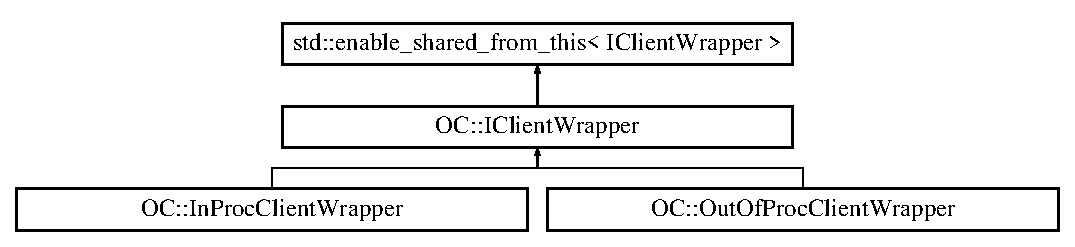
\includegraphics[height=2.876712cm]{classOC_1_1IClientWrapper}
\end{center}
\end{figure}
\subsection*{Public Types}
\begin{DoxyCompactItemize}
\item 
\hypertarget{classOC_1_1IClientWrapper_ae5e1157742c91da0f59e75fc3ae8be45}{}typedef std\+::shared\+\_\+ptr$<$ \hyperlink{classOC_1_1IClientWrapper}{I\+Client\+Wrapper} $>$ {\bfseries Ptr}\label{classOC_1_1IClientWrapper_ae5e1157742c91da0f59e75fc3ae8be45}

\end{DoxyCompactItemize}
\subsection*{Public Member Functions}
\begin{DoxyCompactItemize}
\item 
\hypertarget{classOC_1_1IClientWrapper_ad012eafe311711ae5a33ebe0d41c3f09}{}virtual O\+C\+Stack\+Result {\bfseries Listen\+For\+Resource} (const std\+::string \&service\+Url, const std\+::string \&resource\+Type, Find\+Callback \&callback)=0\label{classOC_1_1IClientWrapper_ad012eafe311711ae5a33ebe0d41c3f09}

\item 
\hypertarget{classOC_1_1IClientWrapper_abefeeea923fed4f9d6bb83fe0d1c8a1e}{}virtual O\+C\+Stack\+Result {\bfseries Get\+Resource\+Attributes} (const std\+::string \&host, const std\+::string \&uri, const Query\+Params\+Map \&query\+Params, Get\+Callback \&callback)=0\label{classOC_1_1IClientWrapper_abefeeea923fed4f9d6bb83fe0d1c8a1e}

\item 
\hypertarget{classOC_1_1IClientWrapper_ad55c3e80b33822504dcbb98139655a34}{}virtual O\+C\+Stack\+Result {\bfseries Set\+Resource\+Attributes} (const std\+::string \&host, const std\+::string \&uri, const \hyperlink{classOC_1_1OCRepresentation}{O\+C\+Representation} \&attributes, const Query\+Params\+Map \&query\+Params, Put\+Callback \&callback)=0\label{classOC_1_1IClientWrapper_ad55c3e80b33822504dcbb98139655a34}

\item 
\hypertarget{classOC_1_1IClientWrapper_a64334f436fb263f50e07a54908f468af}{}virtual O\+C\+Stack\+Result {\bfseries Observe\+Resource} (Observe\+Type observe\+Type, O\+C\+Do\+Handle $\ast$handle, const std\+::string \&host, const std\+::string \&uri, const Query\+Params\+Map \&query\+Params, Observe\+Callback \&callback)=0\label{classOC_1_1IClientWrapper_a64334f436fb263f50e07a54908f468af}

\item 
\hypertarget{classOC_1_1IClientWrapper_a1404240f1bd3efb05f0fbed032fe5a78}{}virtual O\+C\+Stack\+Result {\bfseries Cancel\+Observe\+Resource} (O\+C\+Do\+Handle handle, const std\+::string \&host, const std\+::string \&uri)=0\label{classOC_1_1IClientWrapper_a1404240f1bd3efb05f0fbed032fe5a78}

\item 
\hypertarget{classOC_1_1IClientWrapper_ac9e687574a99db40ce773f0f7ff1d067}{}virtual O\+C\+Stack\+Result {\bfseries Subscribe\+Presence} (O\+C\+Do\+Handle $\ast$handle, const std\+::string \&host, Subscribe\+Callback \&presence\+Handler)=0\label{classOC_1_1IClientWrapper_ac9e687574a99db40ce773f0f7ff1d067}

\item 
\hypertarget{classOC_1_1IClientWrapper_a6fc9f90a5a0b73acddd8088aa0c35fe1}{}virtual O\+C\+Stack\+Result {\bfseries Unsubscribe\+Presence} (O\+C\+Do\+Handle handle)=0\label{classOC_1_1IClientWrapper_a6fc9f90a5a0b73acddd8088aa0c35fe1}

\item 
\hypertarget{classOC_1_1IClientWrapper_a2d644e6bf3b8e54950892947c9db6166}{}virtual std\+::shared\+\_\+ptr$<$ \hyperlink{classOC_1_1OCResource}{O\+C\+Resource} $>$ {\bfseries parse\+O\+C\+Resource} (I\+Client\+Wrapper\+::\+Ptr client\+Wrapper, const std\+::string \&host, const boost\+::property\+\_\+tree\+::ptree resource\+Node)=0\label{classOC_1_1IClientWrapper_a2d644e6bf3b8e54950892947c9db6166}

\end{DoxyCompactItemize}


The documentation for this class was generated from the following file\+:\begin{DoxyCompactItemize}
\item 
/home/user/\+O\+I\+C/oic-\/resource/include/I\+Client\+Wrapper.\+h\end{DoxyCompactItemize}

\hypertarget{classOC_1_1InitializeException}{}\section{O\+C\+:\+:Initialize\+Exception Class Reference}
\label{classOC_1_1InitializeException}\index{O\+C\+::\+Initialize\+Exception@{O\+C\+::\+Initialize\+Exception}}
Inheritance diagram for O\+C\+:\+:Initialize\+Exception\+:\begin{figure}[H]
\begin{center}
\leavevmode
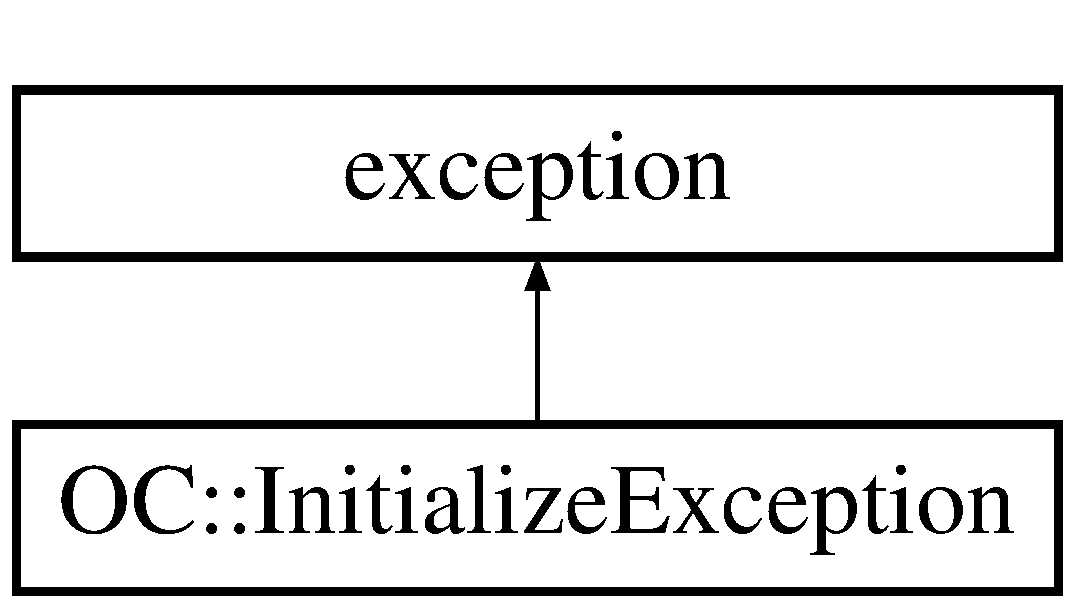
\includegraphics[height=2.000000cm]{classOC_1_1InitializeException}
\end{center}
\end{figure}
\subsection*{Public Member Functions}
\begin{DoxyCompactItemize}
\item 
\hypertarget{classOC_1_1InitializeException_ae1382f57abb002b31e86d43bcc205b61}{}{\bfseries Initialize\+Exception} (const std\+::string \&msg, O\+C\+Stack\+Result reason\+Code)\label{classOC_1_1InitializeException_ae1382f57abb002b31e86d43bcc205b61}

\item 
\hypertarget{classOC_1_1InitializeException_ad9cbcd5ea5edcbee2f7a77cee6d40159}{}O\+C\+Stack\+Result {\bfseries Reason\+Code} ()\label{classOC_1_1InitializeException_ad9cbcd5ea5edcbee2f7a77cee6d40159}

\item 
\hypertarget{classOC_1_1InitializeException_a1bf3ad555a5515d5def6294bf15fc20c}{}std\+::string {\bfseries Message} ()\label{classOC_1_1InitializeException_a1bf3ad555a5515d5def6294bf15fc20c}

\item 
\hypertarget{classOC_1_1InitializeException_a357ac2415acc1215db488291820c770c}{}std\+::string {\bfseries Reason} ()\label{classOC_1_1InitializeException_a357ac2415acc1215db488291820c770c}

\end{DoxyCompactItemize}


The documentation for this class was generated from the following file\+:\begin{DoxyCompactItemize}
\item 
/home/user/\+O\+I\+C/oic-\/resource/include/Initialize\+Exception.\+h\end{DoxyCompactItemize}

\hypertarget{classOC_1_1InProcClientWrapper}{}\section{O\+C\+:\+:In\+Proc\+Client\+Wrapper Class Reference}
\label{classOC_1_1InProcClientWrapper}\index{O\+C\+::\+In\+Proc\+Client\+Wrapper@{O\+C\+::\+In\+Proc\+Client\+Wrapper}}
Inheritance diagram for O\+C\+:\+:In\+Proc\+Client\+Wrapper\+:\begin{figure}[H]
\begin{center}
\leavevmode
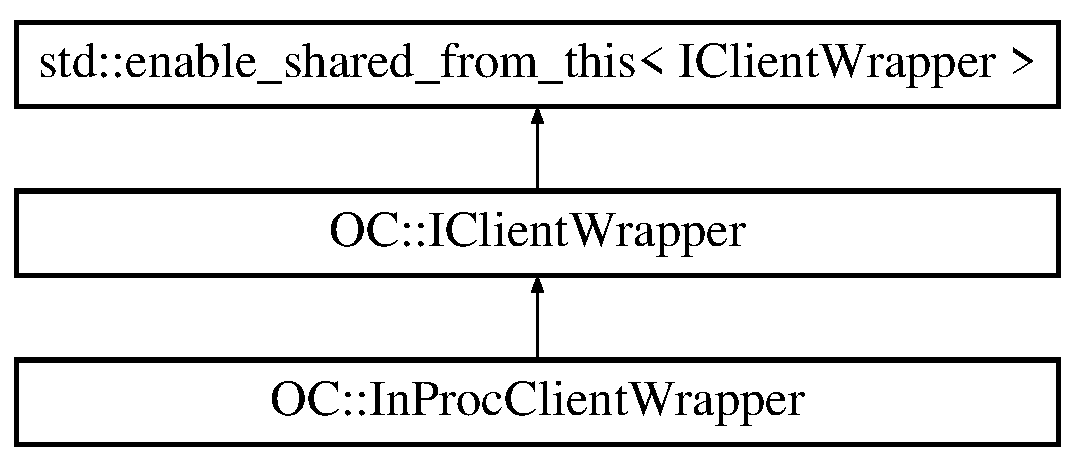
\includegraphics[height=3.000000cm]{classOC_1_1InProcClientWrapper}
\end{center}
\end{figure}
\subsection*{Public Member Functions}
\begin{DoxyCompactItemize}
\item 
\hypertarget{classOC_1_1InProcClientWrapper_a2966d3f07af9340453c0e3e4b5e4b8cd}{}{\bfseries In\+Proc\+Client\+Wrapper} (std\+::weak\+\_\+ptr$<$ std\+::mutex $>$ csdk\+Lock, \hyperlink{structOC_1_1PlatformConfig}{Platform\+Config} cfg)\label{classOC_1_1InProcClientWrapper_a2966d3f07af9340453c0e3e4b5e4b8cd}

\item 
\hypertarget{classOC_1_1InProcClientWrapper_a6e701ab260a3b07f86e5baeafce9f989}{}virtual O\+C\+Stack\+Result {\bfseries Listen\+For\+Resource} (const std\+::string \&service\+Url, const std\+::string \&resource\+Type, Find\+Callback \&callback)\label{classOC_1_1InProcClientWrapper_a6e701ab260a3b07f86e5baeafce9f989}

\item 
\hypertarget{classOC_1_1InProcClientWrapper_a25d5b168f2eb4823ac40e0d615a85864}{}virtual O\+C\+Stack\+Result {\bfseries Get\+Resource\+Attributes} (const std\+::string \&host, const std\+::string \&uri, const Query\+Params\+Map \&query\+Params, Get\+Callback \&callback)\label{classOC_1_1InProcClientWrapper_a25d5b168f2eb4823ac40e0d615a85864}

\item 
\hypertarget{classOC_1_1InProcClientWrapper_aea8548cec4ab7de12b7247592e40cd8d}{}virtual O\+C\+Stack\+Result {\bfseries Set\+Resource\+Attributes} (const std\+::string \&host, const std\+::string \&uri, const \hyperlink{classOC_1_1OCRepresentation}{O\+C\+Representation} \&attributes, const Query\+Params\+Map \&query\+Params, Put\+Callback \&callback)\label{classOC_1_1InProcClientWrapper_aea8548cec4ab7de12b7247592e40cd8d}

\item 
\hypertarget{classOC_1_1InProcClientWrapper_a38493494ea5a2049a076aea85466e2b5}{}virtual O\+C\+Stack\+Result {\bfseries Observe\+Resource} (Observe\+Type observe\+Type, O\+C\+Do\+Handle $\ast$handle, const std\+::string \&host, const std\+::string \&uri, const Query\+Params\+Map \&query\+Params, Observe\+Callback \&callback)\label{classOC_1_1InProcClientWrapper_a38493494ea5a2049a076aea85466e2b5}

\item 
\hypertarget{classOC_1_1InProcClientWrapper_accbae5371c7c5786b6907da6ed634c52}{}virtual O\+C\+Stack\+Result {\bfseries Cancel\+Observe\+Resource} (O\+C\+Do\+Handle handle, const std\+::string \&host, const std\+::string \&uri)\label{classOC_1_1InProcClientWrapper_accbae5371c7c5786b6907da6ed634c52}

\item 
\hypertarget{classOC_1_1InProcClientWrapper_a6515f00b1d0c8e1daf85e12f703851c5}{}virtual O\+C\+Stack\+Result {\bfseries Subscribe\+Presence} (O\+C\+Do\+Handle $\ast$handle, const std\+::string \&host, Subscribe\+Callback \&presence\+Handler)\label{classOC_1_1InProcClientWrapper_a6515f00b1d0c8e1daf85e12f703851c5}

\item 
\hypertarget{classOC_1_1InProcClientWrapper_adbc3490fed3f37b3d6bb1e8c24657a99}{}virtual O\+C\+Stack\+Result {\bfseries Unsubscribe\+Presence} (O\+C\+Do\+Handle handle)\label{classOC_1_1InProcClientWrapper_adbc3490fed3f37b3d6bb1e8c24657a99}

\item 
\hypertarget{classOC_1_1InProcClientWrapper_af1b68c884a253262ac297966354ffecf}{}virtual std\+::shared\+\_\+ptr$<$ \hyperlink{classOC_1_1OCResource}{O\+C\+Resource} $>$ {\bfseries parse\+O\+C\+Resource} (I\+Client\+Wrapper\+::\+Ptr client\+Wrapper, const std\+::string \&host, const boost\+::property\+\_\+tree\+::ptree resource\+Node)\label{classOC_1_1InProcClientWrapper_af1b68c884a253262ac297966354ffecf}

\end{DoxyCompactItemize}
\subsection*{Additional Inherited Members}


The documentation for this class was generated from the following file\+:\begin{DoxyCompactItemize}
\item 
/home/user/\+O\+I\+C/oic-\/resource/include/In\+Proc\+Client\+Wrapper.\+h\end{DoxyCompactItemize}

\hypertarget{classOC_1_1InProcServerWrapper}{}\section{O\+C\+:\+:In\+Proc\+Server\+Wrapper Class Reference}
\label{classOC_1_1InProcServerWrapper}\index{O\+C\+::\+In\+Proc\+Server\+Wrapper@{O\+C\+::\+In\+Proc\+Server\+Wrapper}}
Inheritance diagram for O\+C\+:\+:In\+Proc\+Server\+Wrapper\+:\begin{figure}[H]
\begin{center}
\leavevmode
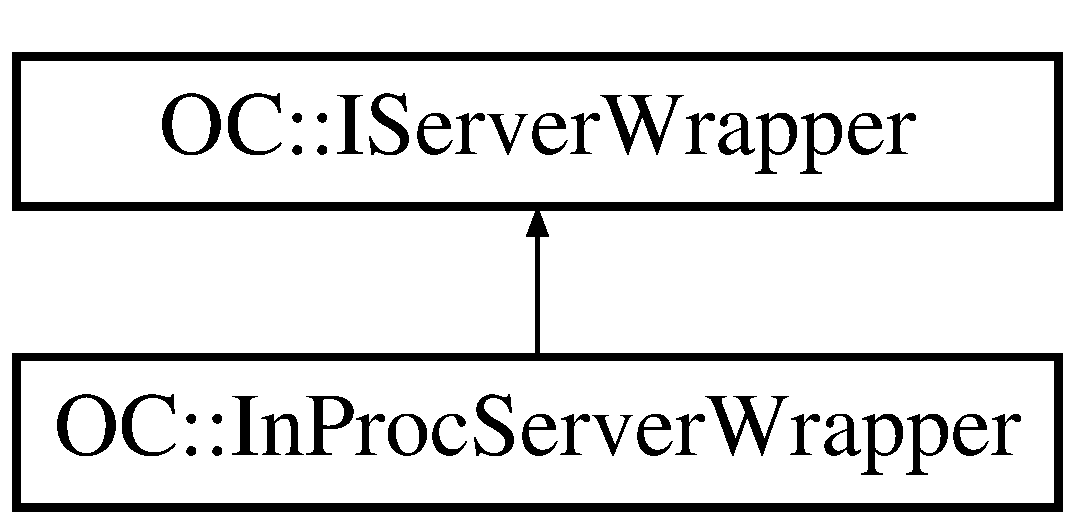
\includegraphics[height=2.000000cm]{classOC_1_1InProcServerWrapper}
\end{center}
\end{figure}
\subsection*{Public Member Functions}
\begin{DoxyCompactItemize}
\item 
\hypertarget{classOC_1_1InProcServerWrapper_a7d57ed7b6fadd5136547470846f432c2}{}{\bfseries In\+Proc\+Server\+Wrapper} (std\+::weak\+\_\+ptr$<$ std\+::mutex $>$ csdk\+Lock, \hyperlink{structOC_1_1PlatformConfig}{Platform\+Config} cfg)\label{classOC_1_1InProcServerWrapper_a7d57ed7b6fadd5136547470846f432c2}

\item 
\hypertarget{classOC_1_1InProcServerWrapper_a1f539d6b9e35e56f585aa181de176d33}{}virtual O\+C\+Stack\+Result {\bfseries register\+Resource} (O\+C\+Resource\+Handle \&resource\+Handle, std\+::string \&resource\+U\+R\+I, const std\+::string \&resource\+Type\+Name, const std\+::string \&resource\+Interface, Register\+Callback \&entity\+Handler, uint8\+\_\+t resource\+Property)\label{classOC_1_1InProcServerWrapper_a1f539d6b9e35e56f585aa181de176d33}

\item 
\hypertarget{classOC_1_1InProcServerWrapper_a4d3186195070f4e3996ae19103bd9940}{}virtual O\+C\+Stack\+Result {\bfseries unregister\+Resource} (const O\+C\+Resource\+Handle \&resource\+Handle)\label{classOC_1_1InProcServerWrapper_a4d3186195070f4e3996ae19103bd9940}

\item 
\hypertarget{classOC_1_1InProcServerWrapper_afd20915bfc9effddccf6bd5f5869d453}{}virtual O\+C\+Stack\+Result {\bfseries bind\+Type\+To\+Resource} (const O\+C\+Resource\+Handle \&resource\+Handle, const std\+::string \&resource\+Type\+Name)\label{classOC_1_1InProcServerWrapper_afd20915bfc9effddccf6bd5f5869d453}

\item 
\hypertarget{classOC_1_1InProcServerWrapper_af8853a36566a2f654d50fccf0782d5f3}{}virtual O\+C\+Stack\+Result {\bfseries bind\+Interface\+To\+Resource} (const O\+C\+Resource\+Handle \&resource\+Handle, const std\+::string \&resource\+Interface)\label{classOC_1_1InProcServerWrapper_af8853a36566a2f654d50fccf0782d5f3}

\item 
\hypertarget{classOC_1_1InProcServerWrapper_a51116f23d4668a00e9f0ccf797f54b72}{}virtual O\+C\+Stack\+Result {\bfseries start\+Presence} (const unsigned int seconds)\label{classOC_1_1InProcServerWrapper_a51116f23d4668a00e9f0ccf797f54b72}

\item 
\hypertarget{classOC_1_1InProcServerWrapper_a831fe208084942ca65b350765cf4902e}{}virtual O\+C\+Stack\+Result {\bfseries stop\+Presence} ()\label{classOC_1_1InProcServerWrapper_a831fe208084942ca65b350765cf4902e}

\end{DoxyCompactItemize}
\subsection*{Additional Inherited Members}


The documentation for this class was generated from the following file\+:\begin{DoxyCompactItemize}
\item 
/home/user/\+O\+I\+C/oic-\/resource/include/In\+Proc\+Server\+Wrapper.\+h\end{DoxyCompactItemize}

\hypertarget{classOC_1_1IServerWrapper}{}\section{O\+C\+:\+:I\+Server\+Wrapper Class Reference}
\label{classOC_1_1IServerWrapper}\index{O\+C\+::\+I\+Server\+Wrapper@{O\+C\+::\+I\+Server\+Wrapper}}
Inheritance diagram for O\+C\+:\+:I\+Server\+Wrapper\+:\begin{figure}[H]
\begin{center}
\leavevmode
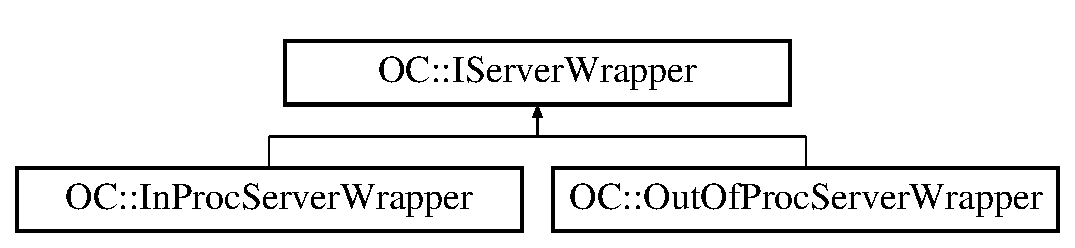
\includegraphics[height=2.000000cm]{classOC_1_1IServerWrapper}
\end{center}
\end{figure}
\subsection*{Public Types}
\begin{DoxyCompactItemize}
\item 
\hypertarget{classOC_1_1IServerWrapper_aa2ec7da5becc94eb6da851384741bbb4}{}typedef std\+::shared\+\_\+ptr$<$ \hyperlink{classOC_1_1IServerWrapper}{I\+Server\+Wrapper} $>$ {\bfseries Ptr}\label{classOC_1_1IServerWrapper_aa2ec7da5becc94eb6da851384741bbb4}

\end{DoxyCompactItemize}
\subsection*{Public Member Functions}
\begin{DoxyCompactItemize}
\item 
\hypertarget{classOC_1_1IServerWrapper_ab67caca25711a77621f8aeabdfaa1c7e}{}virtual O\+C\+Stack\+Result {\bfseries register\+Resource} (O\+C\+Resource\+Handle \&resource\+Handle, std\+::string \&resource\+U\+R\+I, const std\+::string \&resource\+Type\+Name, const std\+::string \&resource\+Interface, Register\+Callback \&entity\+Handler, uint8\+\_\+t resource\+Property)=0\label{classOC_1_1IServerWrapper_ab67caca25711a77621f8aeabdfaa1c7e}

\item 
\hypertarget{classOC_1_1IServerWrapper_a50a7417ac6b067bf6af5a6fbc8ebbbf1}{}virtual O\+C\+Stack\+Result {\bfseries unregister\+Resource} (const O\+C\+Resource\+Handle \&resource\+Handle)=0\label{classOC_1_1IServerWrapper_a50a7417ac6b067bf6af5a6fbc8ebbbf1}

\item 
\hypertarget{classOC_1_1IServerWrapper_a1a5d48597c547fa1f8121e2436adb86b}{}virtual O\+C\+Stack\+Result {\bfseries bind\+Type\+To\+Resource} (const O\+C\+Resource\+Handle \&resource\+Handle, const std\+::string \&resource\+Type\+Name)=0\label{classOC_1_1IServerWrapper_a1a5d48597c547fa1f8121e2436adb86b}

\item 
\hypertarget{classOC_1_1IServerWrapper_a84ad5609491fb426d464b7906a9b9a68}{}virtual O\+C\+Stack\+Result {\bfseries bind\+Interface\+To\+Resource} (const O\+C\+Resource\+Handle \&resource\+Handle, const std\+::string \&resource\+Interface\+Name)=0\label{classOC_1_1IServerWrapper_a84ad5609491fb426d464b7906a9b9a68}

\item 
\hypertarget{classOC_1_1IServerWrapper_a6715a74f2accdfbb59016c76e921251c}{}virtual O\+C\+Stack\+Result {\bfseries start\+Presence} (const unsigned int seconds)=0\label{classOC_1_1IServerWrapper_a6715a74f2accdfbb59016c76e921251c}

\item 
\hypertarget{classOC_1_1IServerWrapper_a59b965cf7f9d16ec8888c42067084caf}{}virtual O\+C\+Stack\+Result {\bfseries stop\+Presence} ()=0\label{classOC_1_1IServerWrapper_a59b965cf7f9d16ec8888c42067084caf}

\end{DoxyCompactItemize}


The documentation for this class was generated from the following file\+:\begin{DoxyCompactItemize}
\item 
/home/user/\+O\+I\+C/oic-\/resource/include/I\+Server\+Wrapper.\+h\end{DoxyCompactItemize}

\hypertarget{classOC_1_1IWrapperFactory}{}\section{O\+C\+:\+:I\+Wrapper\+Factory Class Reference}
\label{classOC_1_1IWrapperFactory}\index{O\+C\+::\+I\+Wrapper\+Factory@{O\+C\+::\+I\+Wrapper\+Factory}}
Inheritance diagram for O\+C\+:\+:I\+Wrapper\+Factory\+:\begin{figure}[H]
\begin{center}
\leavevmode
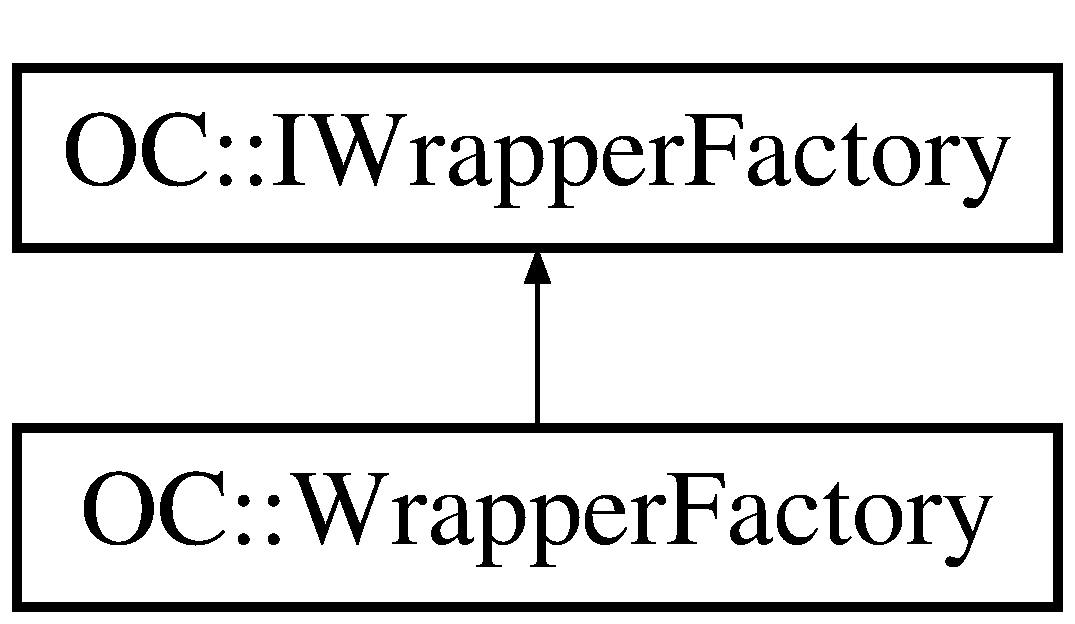
\includegraphics[height=2.000000cm]{classOC_1_1IWrapperFactory}
\end{center}
\end{figure}
\subsection*{Public Types}
\begin{DoxyCompactItemize}
\item 
\hypertarget{classOC_1_1IWrapperFactory_aa652203fa13f2f4651c10d2c09dd48d6}{}typedef std\+::shared\+\_\+ptr$<$ \hyperlink{classOC_1_1IWrapperFactory}{I\+Wrapper\+Factory} $>$ {\bfseries Ptr}\label{classOC_1_1IWrapperFactory_aa652203fa13f2f4651c10d2c09dd48d6}

\end{DoxyCompactItemize}
\subsection*{Public Member Functions}
\begin{DoxyCompactItemize}
\item 
\hypertarget{classOC_1_1IWrapperFactory_a99bbd34dc0390b75efd5b5de55fb6352}{}virtual I\+Client\+Wrapper\+::\+Ptr {\bfseries Create\+Client\+Wrapper} (std\+::weak\+\_\+ptr$<$ std\+::mutex $>$ csdk\+Lock, \hyperlink{structOC_1_1PlatformConfig}{Platform\+Config} cfg)=0\label{classOC_1_1IWrapperFactory_a99bbd34dc0390b75efd5b5de55fb6352}

\item 
\hypertarget{classOC_1_1IWrapperFactory_a25a4cb7ca863c34f408791380ced127f}{}virtual I\+Server\+Wrapper\+::\+Ptr {\bfseries Create\+Server\+Wrapper} (std\+::weak\+\_\+ptr$<$ std\+::mutex $>$ csdk\+Lock, \hyperlink{structOC_1_1PlatformConfig}{Platform\+Config} cfg)=0\label{classOC_1_1IWrapperFactory_a25a4cb7ca863c34f408791380ced127f}

\end{DoxyCompactItemize}


The documentation for this class was generated from the following file\+:\begin{DoxyCompactItemize}
\item 
/home/user/\+O\+I\+C/oic-\/resource/include/Wrapper\+Factory.\+h\end{DoxyCompactItemize}

\hypertarget{structlist}{}\section{list Struct Reference}
\label{structlist}\index{list@{list}}
\subsection*{Public Attributes}
\begin{DoxyCompactItemize}
\item 
\hypertarget{structlist_a1900fe79e875e2838625b2eb60837f8f}{}struct \hyperlink{structlist}{list} $\ast$ {\bfseries next}\label{structlist_a1900fe79e875e2838625b2eb60837f8f}

\end{DoxyCompactItemize}


The documentation for this struct was generated from the following file\+:\begin{DoxyCompactItemize}
\item 
/home/user/\+O\+I\+C/oic-\/resource/csdk/libcoap-\/4.\+1.\+1/\hyperlink{t__list_8h}{t\+\_\+list.\+h}\end{DoxyCompactItemize}

\hypertarget{classremoting_1_1LiteConnection}{}\section{remoting\+:\+:Lite\+Connection Class Reference}
\label{classremoting_1_1LiteConnection}\index{remoting\+::\+Lite\+Connection@{remoting\+::\+Lite\+Connection}}
\subsection*{Public Member Functions}
\begin{DoxyCompactItemize}
\item 
\hypertarget{classremoting_1_1LiteConnection_ab028f9c2637f493a933640ecd76afb82}{}{\bfseries Lite\+Connection} (int socket)\label{classremoting_1_1LiteConnection_ab028f9c2637f493a933640ecd76afb82}

\end{DoxyCompactItemize}


The documentation for this class was generated from the following file\+:\begin{DoxyCompactItemize}
\item 
/home/user/\+O\+I\+C/oic-\/resource/csdk/controller/src/remoting/Lite\+Connection.\+h\end{DoxyCompactItemize}

\hypertarget{classremoting_1_1LiteRemoting}{}\section{remoting\+:\+:Lite\+Remoting Class Reference}
\label{classremoting_1_1LiteRemoting}\index{remoting\+::\+Lite\+Remoting@{remoting\+::\+Lite\+Remoting}}
\subsection*{Public Types}
\begin{DoxyCompactItemize}
\item 
\hypertarget{classremoting_1_1LiteRemoting_acb133b1bca11b2788b3f40775a44ee39}{}typedef boost\+::shared\+\_\+ptr$<$ \hyperlink{classremoting_1_1LiteRemoting}{Lite\+Remoting} $>$ {\bfseries Ptr}\label{classremoting_1_1LiteRemoting_acb133b1bca11b2788b3f40775a44ee39}

\end{DoxyCompactItemize}
\subsection*{Public Member Functions}
\begin{DoxyCompactItemize}
\item 
\hypertarget{classremoting_1_1LiteRemoting_a02062ef11ead93d148bb509356e571c0}{}{\bfseries Lite\+Remoting} (Private\+Construct\+Key key)\label{classremoting_1_1LiteRemoting_a02062ef11ead93d148bb509356e571c0}

\end{DoxyCompactItemize}
\subsection*{Static Public Member Functions}
\begin{DoxyCompactItemize}
\item 
\hypertarget{classremoting_1_1LiteRemoting_a1f7a788b63d3a0839b692b4bbc1d9a7a}{}static boost\+::shared\+\_\+ptr$<$ \hyperlink{classremoting_1_1LiteRemoting}{Lite\+Remoting} $>$ {\bfseries get\+Instance} ()\label{classremoting_1_1LiteRemoting_a1f7a788b63d3a0839b692b4bbc1d9a7a}

\end{DoxyCompactItemize}
\subsection*{Static Public Attributes}
\begin{DoxyCompactItemize}
\item 
\hypertarget{classremoting_1_1LiteRemoting_a487c73741c3586a78acd0816558fe490}{}static const std\+::string {\bfseries A\+P\+P\+L\+I\+C\+A\+T\+I\+O\+N\+\_\+\+U\+U\+I\+D\+\_\+\+S\+T\+R\+I\+N\+G}\label{classremoting_1_1LiteRemoting_a487c73741c3586a78acd0816558fe490}

\end{DoxyCompactItemize}


The documentation for this class was generated from the following file\+:\begin{DoxyCompactItemize}
\item 
/home/user/\+O\+I\+C/oic-\/resource/csdk/controller/src/remoting/Lite\+Remoting.\+h\end{DoxyCompactItemize}

\hypertarget{classremoting_1_1LiteSessionImpl}{}\section{remoting\+:\+:Lite\+Session\+Impl Class Reference}
\label{classremoting_1_1LiteSessionImpl}\index{remoting\+::\+Lite\+Session\+Impl@{remoting\+::\+Lite\+Session\+Impl}}
Inheritance diagram for remoting\+:\+:Lite\+Session\+Impl\+:\begin{figure}[H]
\begin{center}
\leavevmode
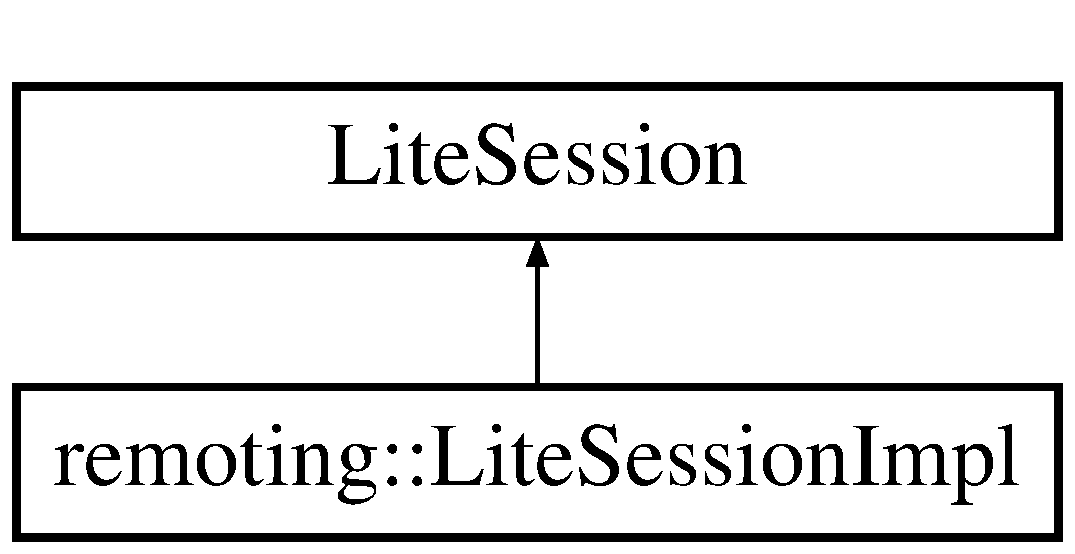
\includegraphics[height=2.000000cm]{classremoting_1_1LiteSessionImpl}
\end{center}
\end{figure}
\subsection*{Public Member Functions}
\begin{DoxyCompactItemize}
\item 
\hypertarget{classremoting_1_1LiteSessionImpl_abfa3ba953f551f2273a261b6d072fd92}{}{\bfseries Lite\+Session\+Impl} (A\+P\+I\+::\+Context\+::\+Shared\+Ptr p\+C\+C\+F\+Context, U\+U\+I\+D\+\_\+t uuid)\label{classremoting_1_1LiteSessionImpl_abfa3ba953f551f2273a261b6d072fd92}

\item 
\hypertarget{classremoting_1_1LiteSessionImpl_a630799c0a68877c1cb97e75ca41127ad}{}virtual void {\bfseries invite} ()\label{classremoting_1_1LiteSessionImpl_a630799c0a68877c1cb97e75ca41127ad}

\item 
\hypertarget{classremoting_1_1LiteSessionImpl_af3e554403b93a5c4b7af1675482a0cf5}{}virtual void {\bfseries disconnect} ()\label{classremoting_1_1LiteSessionImpl_af3e554403b93a5c4b7af1675482a0cf5}

\end{DoxyCompactItemize}


The documentation for this class was generated from the following file\+:\begin{DoxyCompactItemize}
\item 
/home/user/\+O\+I\+C/oic-\/resource/csdk/controller/src/remoting/Lite\+Session\+Impl.\+h\end{DoxyCompactItemize}

\hypertarget{classremoting_1_1LiteTargetDeviceProxy}{}\section{remoting\+:\+:Lite\+Target\+Device\+Proxy Class Reference}
\label{classremoting_1_1LiteTargetDeviceProxy}\index{remoting\+::\+Lite\+Target\+Device\+Proxy@{remoting\+::\+Lite\+Target\+Device\+Proxy}}
Inheritance diagram for remoting\+:\+:Lite\+Target\+Device\+Proxy\+:\begin{figure}[H]
\begin{center}
\leavevmode
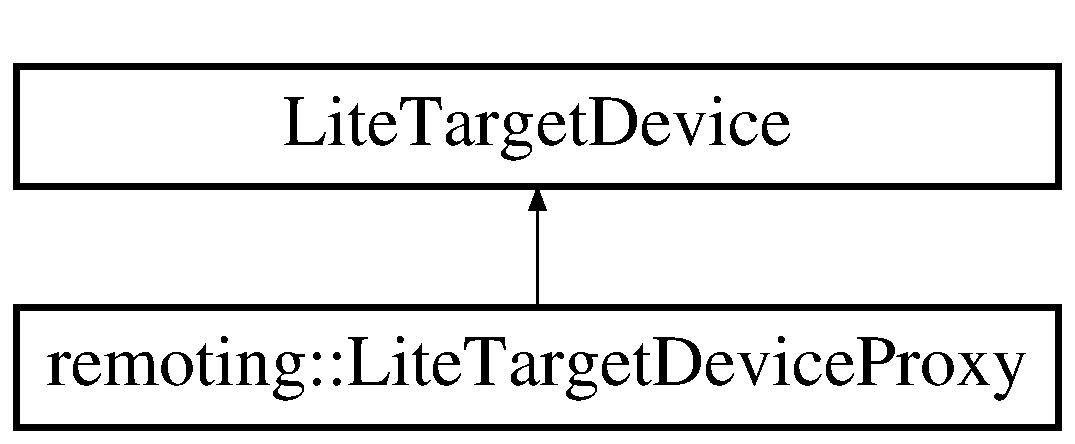
\includegraphics[height=2.000000cm]{classremoting_1_1LiteTargetDeviceProxy}
\end{center}
\end{figure}
\subsection*{Public Member Functions}
\begin{DoxyCompactItemize}
\item 
\hypertarget{classremoting_1_1LiteTargetDeviceProxy_aba6f2d0a8312fedefa2bbaca24e9aea2}{}{\bfseries Lite\+Target\+Device\+Proxy} (U\+U\+I\+D\+\_\+t uuid)\label{classremoting_1_1LiteTargetDeviceProxy_aba6f2d0a8312fedefa2bbaca24e9aea2}

\end{DoxyCompactItemize}


The documentation for this class was generated from the following file\+:\begin{DoxyCompactItemize}
\item 
/home/user/\+O\+I\+C/oic-\/resource/csdk/controller/src/remoting/Lite\+Target\+Device\+Proxy.\+h\end{DoxyCompactItemize}

\hypertarget{classIntel_1_1CCFL_1_1Protocols_1_1MockProtocol}{}\section{Intel\+:\+:C\+C\+F\+L\+:\+:Protocols\+:\+:Mock\+Protocol Class Reference}
\label{classIntel_1_1CCFL_1_1Protocols_1_1MockProtocol}\index{Intel\+::\+C\+C\+F\+L\+::\+Protocols\+::\+Mock\+Protocol@{Intel\+::\+C\+C\+F\+L\+::\+Protocols\+::\+Mock\+Protocol}}
Inheritance diagram for Intel\+:\+:C\+C\+F\+L\+:\+:Protocols\+:\+:Mock\+Protocol\+:\begin{figure}[H]
\begin{center}
\leavevmode
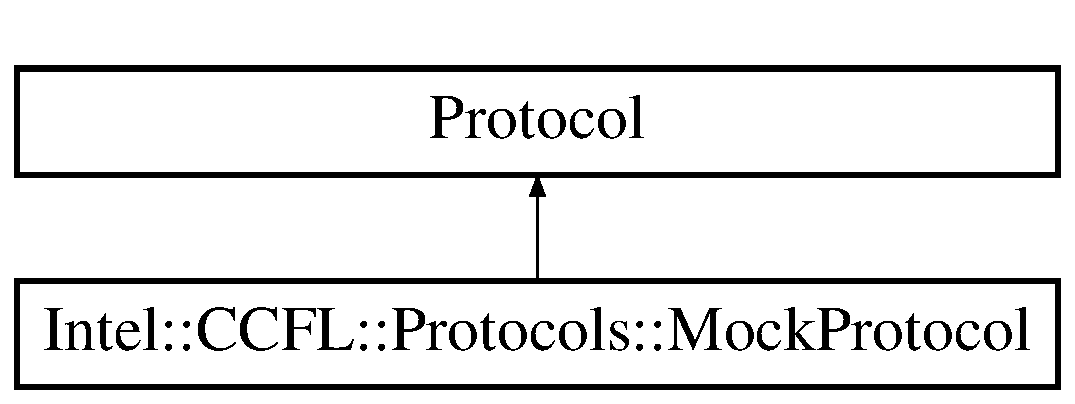
\includegraphics[height=2.000000cm]{classIntel_1_1CCFL_1_1Protocols_1_1MockProtocol}
\end{center}
\end{figure}
\subsection*{Public Member Functions}
\begin{DoxyCompactItemize}
\item 
\hypertarget{classIntel_1_1CCFL_1_1Protocols_1_1MockProtocol_ad2125b0370d6eddb2b7f9c3afaad38d4}{}virtual void {\bfseries set\+Model} (const std\+::shared\+\_\+ptr$<$ \hyperlink{classIntel_1_1CCFL_1_1API_1_1Model}{Intel\+::\+C\+C\+F\+L\+::\+A\+P\+I\+::\+Model} $>$ \&model)\label{classIntel_1_1CCFL_1_1Protocols_1_1MockProtocol_ad2125b0370d6eddb2b7f9c3afaad38d4}

\item 
\hypertarget{classIntel_1_1CCFL_1_1Protocols_1_1MockProtocol_accc8ad01d36bddaadbf329e3d6c51374}{}virtual const Handle {\bfseries get\+Handle} ()\label{classIntel_1_1CCFL_1_1Protocols_1_1MockProtocol_accc8ad01d36bddaadbf329e3d6c51374}

\item 
\hypertarget{classIntel_1_1CCFL_1_1Protocols_1_1MockProtocol_a5e1bd8e3536bc5dabcf41e3807b810ea}{}virtual void {\bfseries set\+Handle} (const Handle handle)\label{classIntel_1_1CCFL_1_1Protocols_1_1MockProtocol_a5e1bd8e3536bc5dabcf41e3807b810ea}

\item 
\hypertarget{classIntel_1_1CCFL_1_1Protocols_1_1MockProtocol_a02c0401faccf57004441ab54a714e436}{}virtual const std\+::string \& {\bfseries get\+Name} ()\label{classIntel_1_1CCFL_1_1Protocols_1_1MockProtocol_a02c0401faccf57004441ab54a714e436}

\item 
\hypertarget{classIntel_1_1CCFL_1_1Protocols_1_1MockProtocol_a0e91bfa3ff7cf400e6ee8108849836f4}{}virtual void {\bfseries set\+Name} (const std\+::string \&name)\label{classIntel_1_1CCFL_1_1Protocols_1_1MockProtocol_a0e91bfa3ff7cf400e6ee8108849836f4}

\item 
\hypertarget{classIntel_1_1CCFL_1_1Protocols_1_1MockProtocol_a22b21c9ed8911e4f3b4f2e470695cded}{}virtual void {\bfseries force\+Device\+Discovery} ()\label{classIntel_1_1CCFL_1_1Protocols_1_1MockProtocol_a22b21c9ed8911e4f3b4f2e470695cded}

\item 
\hypertarget{classIntel_1_1CCFL_1_1Protocols_1_1MockProtocol_a1e8012f43b726201462bbc290ac00b94}{}void {\bfseries test\+Add\+Device} (const U\+U\+I\+D\+\_\+t \&device\+Id, const std\+::string device\+Name)\label{classIntel_1_1CCFL_1_1Protocols_1_1MockProtocol_a1e8012f43b726201462bbc290ac00b94}

\item 
\hypertarget{classIntel_1_1CCFL_1_1Protocols_1_1MockProtocol_aef8146348057c7e28cfd0d5974aa04be}{}void {\bfseries test\+Remove\+Device} (const U\+U\+I\+D\+\_\+t \&device\+Id)\label{classIntel_1_1CCFL_1_1Protocols_1_1MockProtocol_aef8146348057c7e28cfd0d5974aa04be}

\end{DoxyCompactItemize}


The documentation for this class was generated from the following file\+:\begin{DoxyCompactItemize}
\item 
/home/user/\+O\+I\+C/oic-\/resource/csdk/controller/core/test/Mock\+Protocol.\+h\end{DoxyCompactItemize}

\hypertarget{classIntel_1_1CCFL_1_1API_1_1Model}{}\section{Intel\+:\+:C\+C\+F\+L\+:\+:A\+P\+I\+:\+:Model Class Reference}
\label{classIntel_1_1CCFL_1_1API_1_1Model}\index{Intel\+::\+C\+C\+F\+L\+::\+A\+P\+I\+::\+Model@{Intel\+::\+C\+C\+F\+L\+::\+A\+P\+I\+::\+Model}}
Inheritance diagram for Intel\+:\+:C\+C\+F\+L\+:\+:A\+P\+I\+:\+:Model\+:\begin{figure}[H]
\begin{center}
\leavevmode
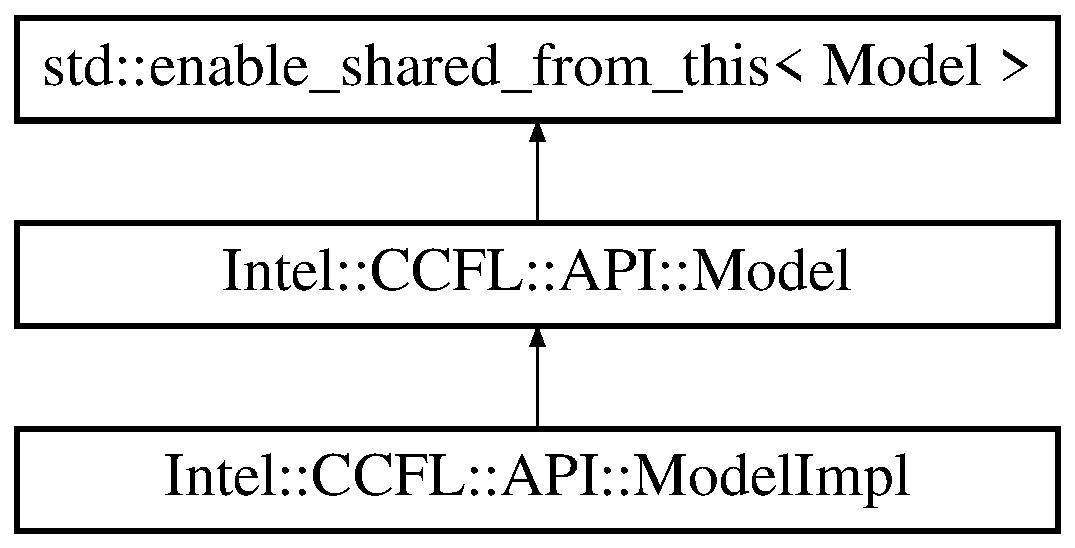
\includegraphics[height=3.000000cm]{classIntel_1_1CCFL_1_1API_1_1Model}
\end{center}
\end{figure}
\subsection*{Public Types}
\begin{DoxyCompactItemize}
\item 
\hypertarget{classIntel_1_1CCFL_1_1API_1_1Model_aa1c5686fbac89152ae6abaabfa8b181a}{}typedef std\+::shared\+\_\+ptr$<$ \hyperlink{classIntel_1_1CCFL_1_1API_1_1Model}{Model} $>$ {\bfseries Shared\+Ptr}\label{classIntel_1_1CCFL_1_1API_1_1Model_aa1c5686fbac89152ae6abaabfa8b181a}

\item 
\hypertarget{classIntel_1_1CCFL_1_1API_1_1Model_adaae0c4043566501c3bcf2a95c09ee52}{}typedef std\+::weak\+\_\+ptr$<$ \hyperlink{classIntel_1_1CCFL_1_1API_1_1Model}{Model} $>$ {\bfseries Weak\+Ptr}\label{classIntel_1_1CCFL_1_1API_1_1Model_adaae0c4043566501c3bcf2a95c09ee52}

\end{DoxyCompactItemize}
\subsection*{Public Member Functions}
\begin{DoxyCompactItemize}
\item 
\hypertarget{classIntel_1_1CCFL_1_1API_1_1Model_a636991fabad8025795534e4800101922}{}virtual void {\bfseries get\+Devices} (Get\+Devices\+Function \&async\+Return\+Func)=0\label{classIntel_1_1CCFL_1_1API_1_1Model_a636991fabad8025795534e4800101922}

\item 
\hypertarget{classIntel_1_1CCFL_1_1API_1_1Model_a779ad03099d8997cb06f90b197fcf42c}{}virtual void {\bfseries remove\+Device\+Observer} (Device\+Observer\+Handle observer\+Handle)=0\label{classIntel_1_1CCFL_1_1API_1_1Model_a779ad03099d8997cb06f90b197fcf42c}

\item 
\hypertarget{classIntel_1_1CCFL_1_1API_1_1Model_a59a3be8d0e67d6afae5d29a8831b03f3}{}virtual void {\bfseries set\+Device\+Observer} (Device\+Event\+Function \&async\+Event\+Function)=0\label{classIntel_1_1CCFL_1_1API_1_1Model_a59a3be8d0e67d6afae5d29a8831b03f3}

\item 
\hypertarget{classIntel_1_1CCFL_1_1API_1_1Model_ace328a0d0425cf25681ce71d55b59da0}{}virtual const Protocols\+::\+Protocol\+::\+Handle {\bfseries register\+Protocol} (const Protocols\+::\+Protocol\+::\+Shared\+Ptr \&protocol)=0\label{classIntel_1_1CCFL_1_1API_1_1Model_ace328a0d0425cf25681ce71d55b59da0}

\item 
\hypertarget{classIntel_1_1CCFL_1_1API_1_1Model_a96b9a6a0fc4399a3af0a3b6bca4ff6ec}{}virtual bool {\bfseries unregister\+Protocol} (const Protocols\+::\+Protocol\+::\+Handle protocol\+Handle)=0\label{classIntel_1_1CCFL_1_1API_1_1Model_a96b9a6a0fc4399a3af0a3b6bca4ff6ec}

\item 
\hypertarget{classIntel_1_1CCFL_1_1API_1_1Model_a47632b120a4a83ac98b4c7d723fc396c}{}virtual Device\+::\+Shared\+Ptr {\bfseries get\+Device} (const U\+U\+I\+D\+\_\+t \&device\+Id)=0\label{classIntel_1_1CCFL_1_1API_1_1Model_a47632b120a4a83ac98b4c7d723fc396c}

\item 
\hypertarget{classIntel_1_1CCFL_1_1API_1_1Model_ae1f154dd5945c98537faadbeb8dbc82c}{}virtual void {\bfseries signal\+Device\+Change} (const U\+U\+I\+D\+\_\+t \&device\+Id, Device\+Event\+::\+Device\+Change device\+Event)=0\label{classIntel_1_1CCFL_1_1API_1_1Model_ae1f154dd5945c98537faadbeb8dbc82c}

\end{DoxyCompactItemize}
\subsection*{Static Public Member Functions}
\begin{DoxyCompactItemize}
\item 
\hypertarget{classIntel_1_1CCFL_1_1API_1_1Model_a8bbb0299941b27d4ec441270daf1cbb2}{}static Shared\+Ptr {\bfseries create\+Model} ()\label{classIntel_1_1CCFL_1_1API_1_1Model_a8bbb0299941b27d4ec441270daf1cbb2}

\end{DoxyCompactItemize}


The documentation for this class was generated from the following file\+:\begin{DoxyCompactItemize}
\item 
/home/user/\+O\+I\+C/oic-\/resource/csdk/controller/core/include/core/Internal\+Api.\+h\end{DoxyCompactItemize}

\hypertarget{classIntel_1_1CCFL_1_1API_1_1ModelImpl}{}\section{Intel\+:\+:C\+C\+F\+L\+:\+:A\+P\+I\+:\+:Model\+Impl Class Reference}
\label{classIntel_1_1CCFL_1_1API_1_1ModelImpl}\index{Intel\+::\+C\+C\+F\+L\+::\+A\+P\+I\+::\+Model\+Impl@{Intel\+::\+C\+C\+F\+L\+::\+A\+P\+I\+::\+Model\+Impl}}
Inheritance diagram for Intel\+:\+:C\+C\+F\+L\+:\+:A\+P\+I\+:\+:Model\+Impl\+:\begin{figure}[H]
\begin{center}
\leavevmode
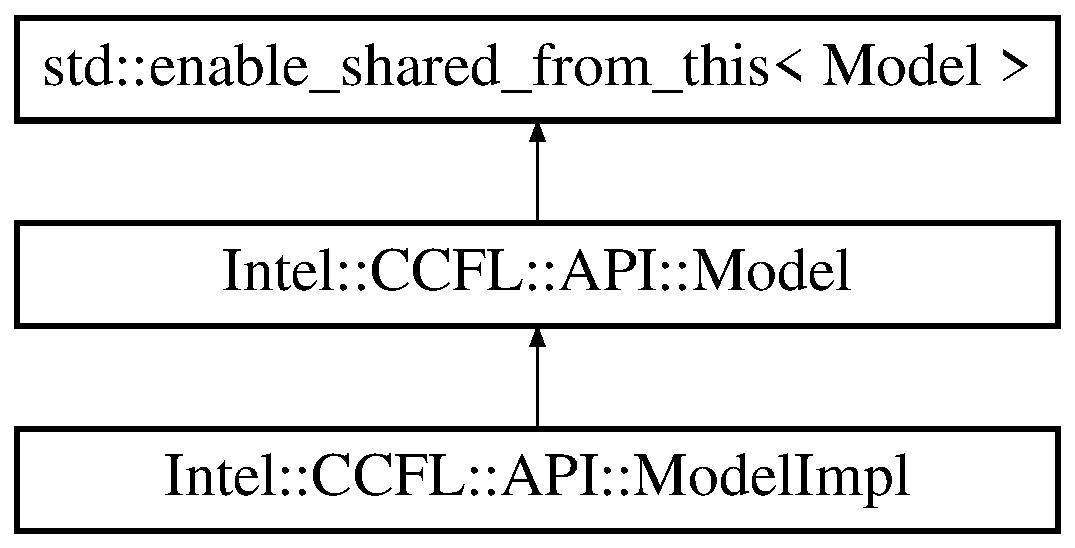
\includegraphics[height=3.000000cm]{classIntel_1_1CCFL_1_1API_1_1ModelImpl}
\end{center}
\end{figure}
\subsection*{Public Types}
\begin{DoxyCompactItemize}
\item 
\hypertarget{classIntel_1_1CCFL_1_1API_1_1ModelImpl_ac2868350b141e5db12f24cbea34afe80}{}typedef std\+::shared\+\_\+ptr$<$ \hyperlink{classIntel_1_1CCFL_1_1API_1_1ModelImpl}{Model\+Impl} $>$ {\bfseries Shared\+Ptr}\label{classIntel_1_1CCFL_1_1API_1_1ModelImpl_ac2868350b141e5db12f24cbea34afe80}

\item 
\hypertarget{classIntel_1_1CCFL_1_1API_1_1ModelImpl_a1cd5a9a00631de73dbc5fc0a523ad5e2}{}typedef std\+::weak\+\_\+ptr$<$ \hyperlink{classIntel_1_1CCFL_1_1API_1_1ModelImpl}{Model\+Impl} $>$ {\bfseries Weak\+Ptr}\label{classIntel_1_1CCFL_1_1API_1_1ModelImpl_a1cd5a9a00631de73dbc5fc0a523ad5e2}

\end{DoxyCompactItemize}
\subsection*{Public Member Functions}
\begin{DoxyCompactItemize}
\item 
\hypertarget{classIntel_1_1CCFL_1_1API_1_1ModelImpl_ac2741dd52f25119cbc6e3567f61bcd25}{}virtual void {\bfseries get\+Devices} (Get\+Devices\+Function \&async\+Return\+Func)\label{classIntel_1_1CCFL_1_1API_1_1ModelImpl_ac2741dd52f25119cbc6e3567f61bcd25}

\item 
\hypertarget{classIntel_1_1CCFL_1_1API_1_1ModelImpl_abf106aae363526292c0a6074ecfe5270}{}virtual void {\bfseries remove\+Device\+Observer} (Device\+Observer\+Handle observer\+Handle)\label{classIntel_1_1CCFL_1_1API_1_1ModelImpl_abf106aae363526292c0a6074ecfe5270}

\item 
\hypertarget{classIntel_1_1CCFL_1_1API_1_1ModelImpl_a91aa9a4d23b95676250ce507a1509d9b}{}virtual void {\bfseries set\+Device\+Observer} (Device\+Event\+Function \&async\+Event\+Function)\label{classIntel_1_1CCFL_1_1API_1_1ModelImpl_a91aa9a4d23b95676250ce507a1509d9b}

\item 
\hypertarget{classIntel_1_1CCFL_1_1API_1_1ModelImpl_a3dc39b19097e564441e933c8bb19290b}{}virtual const Protocols\+::\+Protocol\+::\+Handle {\bfseries register\+Protocol} (const Protocols\+::\+Protocol\+::\+Shared\+Ptr \&protocol)\label{classIntel_1_1CCFL_1_1API_1_1ModelImpl_a3dc39b19097e564441e933c8bb19290b}

\item 
\hypertarget{classIntel_1_1CCFL_1_1API_1_1ModelImpl_ae16e99e2682a4ab3ccd1296db5c27360}{}virtual bool {\bfseries unregister\+Protocol} (const Protocols\+::\+Protocol\+::\+Handle protocol\+Handle)\label{classIntel_1_1CCFL_1_1API_1_1ModelImpl_ae16e99e2682a4ab3ccd1296db5c27360}

\item 
\hypertarget{classIntel_1_1CCFL_1_1API_1_1ModelImpl_a598202ad4e608bd8c8308db922438fa0}{}virtual Device\+::\+Shared\+Ptr {\bfseries get\+Device} (const U\+U\+I\+D\+\_\+t \&device\+Id)\label{classIntel_1_1CCFL_1_1API_1_1ModelImpl_a598202ad4e608bd8c8308db922438fa0}

\item 
\hypertarget{classIntel_1_1CCFL_1_1API_1_1ModelImpl_aa8f124028e8143e132928acfced3eeaf}{}virtual void {\bfseries signal\+Device\+Change} (const U\+U\+I\+D\+\_\+t \&device\+Id, Device\+Event\+::\+Device\+Change device\+Event)\label{classIntel_1_1CCFL_1_1API_1_1ModelImpl_aa8f124028e8143e132928acfced3eeaf}

\end{DoxyCompactItemize}
\subsection*{Static Public Member Functions}
\begin{DoxyCompactItemize}
\item 
\hypertarget{classIntel_1_1CCFL_1_1API_1_1ModelImpl_a11fe1a81c087bdcfccf506a9d0b34b1f}{}static Shared\+Ptr {\bfseries create\+Model} ()\label{classIntel_1_1CCFL_1_1API_1_1ModelImpl_a11fe1a81c087bdcfccf506a9d0b34b1f}

\end{DoxyCompactItemize}


The documentation for this class was generated from the following file\+:\begin{DoxyCompactItemize}
\item 
/home/user/\+O\+I\+C/oic-\/resource/csdk/controller/core/src/Model\+Impl.\+h\end{DoxyCompactItemize}

\hypertarget{classOC_1_1MyMultiResourceHandler}{}\section{O\+C\+:\+:My\+Multi\+Resource\+Handler Class Reference}
\label{classOC_1_1MyMultiResourceHandler}\index{O\+C\+::\+My\+Multi\+Resource\+Handler@{O\+C\+::\+My\+Multi\+Resource\+Handler}}
Inheritance diagram for O\+C\+:\+:My\+Multi\+Resource\+Handler\+:\begin{figure}[H]
\begin{center}
\leavevmode
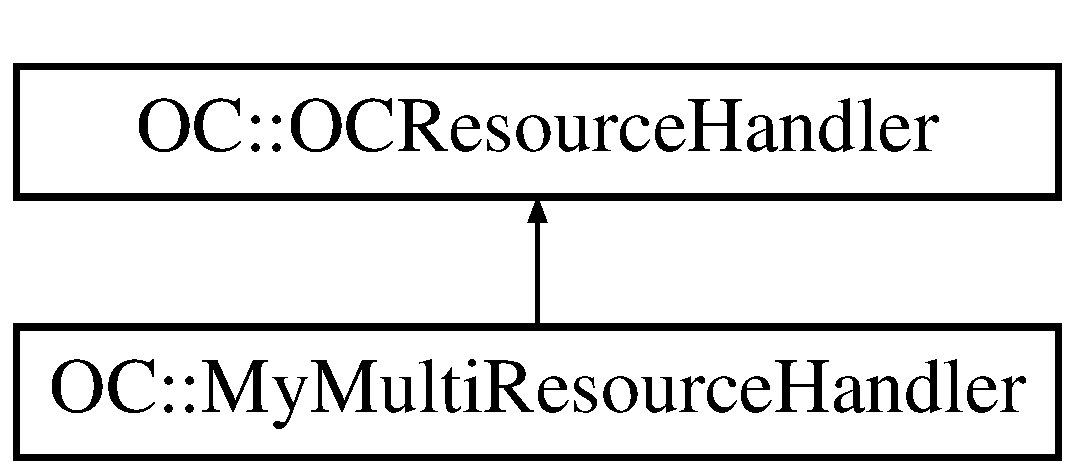
\includegraphics[height=2.000000cm]{classOC_1_1MyMultiResourceHandler}
\end{center}
\end{figure}
\subsection*{Public Member Functions}
\begin{DoxyCompactItemize}
\item 
\hypertarget{classOC_1_1MyMultiResourceHandler_a542edaaedfc1c7bc25a4dba4b7f56b66}{}void {\bfseries on\+Found\+Resource} (O\+C\+Resource\+Result $\ast$update, void $\ast$params)\label{classOC_1_1MyMultiResourceHandler_a542edaaedfc1c7bc25a4dba4b7f56b66}

\item 
\hypertarget{classOC_1_1MyMultiResourceHandler_a3472b8a1bc575a39a984f05a5bdfc390}{}void {\bfseries on\+Completed} ()\label{classOC_1_1MyMultiResourceHandler_a3472b8a1bc575a39a984f05a5bdfc390}

\item 
\hypertarget{classOC_1_1MyMultiResourceHandler_ac1cecae8532c84dbf7ac07c37e07e6f6}{}void {\bfseries on\+Failed} ()\label{classOC_1_1MyMultiResourceHandler_ac1cecae8532c84dbf7ac07c37e07e6f6}

\end{DoxyCompactItemize}


The documentation for this class was generated from the following file\+:\begin{DoxyCompactItemize}
\item 
/home/user/\+O\+I\+C/oic-\/resource/examples/old\+\_\+tests/My\+Multi\+Resource\+Handler.\+h\end{DoxyCompactItemize}

\hypertarget{classOC_1_1MyObserverHandler}{}\section{O\+C\+:\+:My\+Observer\+Handler Class Reference}
\label{classOC_1_1MyObserverHandler}\index{O\+C\+::\+My\+Observer\+Handler@{O\+C\+::\+My\+Observer\+Handler}}
Inheritance diagram for O\+C\+:\+:My\+Observer\+Handler\+:\begin{figure}[H]
\begin{center}
\leavevmode
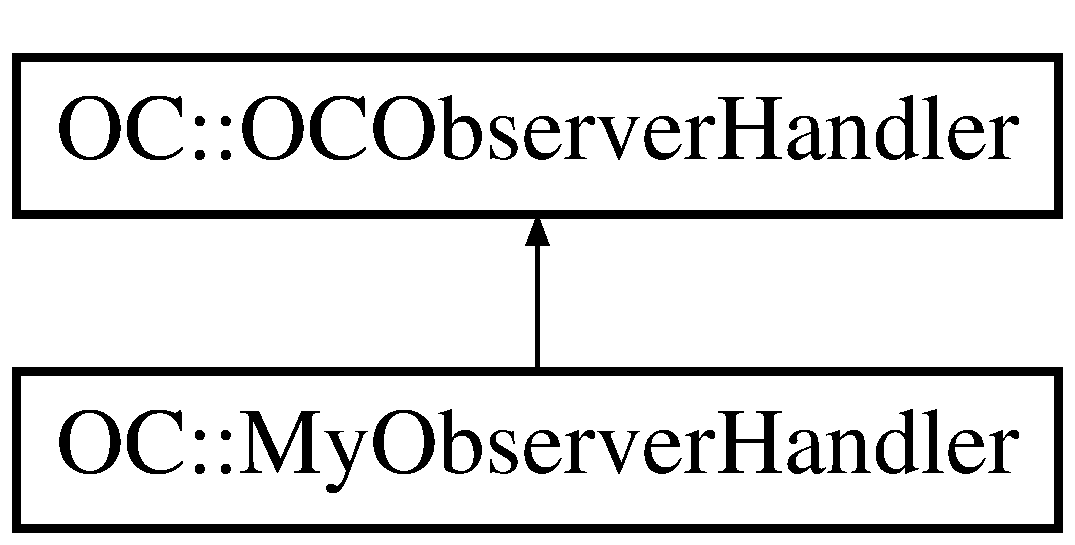
\includegraphics[height=2.000000cm]{classOC_1_1MyObserverHandler}
\end{center}
\end{figure}
\subsection*{Public Member Functions}
\begin{DoxyCompactItemize}
\item 
\hypertarget{classOC_1_1MyObserverHandler_a8aeabd5306be9576ef7c21abb6df3b0a}{}void {\bfseries on\+Observer\+Update} (std\+::string property\+Name, void $\ast$value)\label{classOC_1_1MyObserverHandler_a8aeabd5306be9576ef7c21abb6df3b0a}

\end{DoxyCompactItemize}


The documentation for this class was generated from the following file\+:\begin{DoxyCompactItemize}
\item 
/home/user/\+O\+I\+C/oic-\/resource/examples/old\+\_\+tests/My\+Observer\+Handler.\+h\end{DoxyCompactItemize}

\hypertarget{classMyResourceHandler}{}\section{My\+Resource\+Handler Class Reference}
\label{classMyResourceHandler}\index{My\+Resource\+Handler@{My\+Resource\+Handler}}
Inheritance diagram for My\+Resource\+Handler\+:\begin{figure}[H]
\begin{center}
\leavevmode
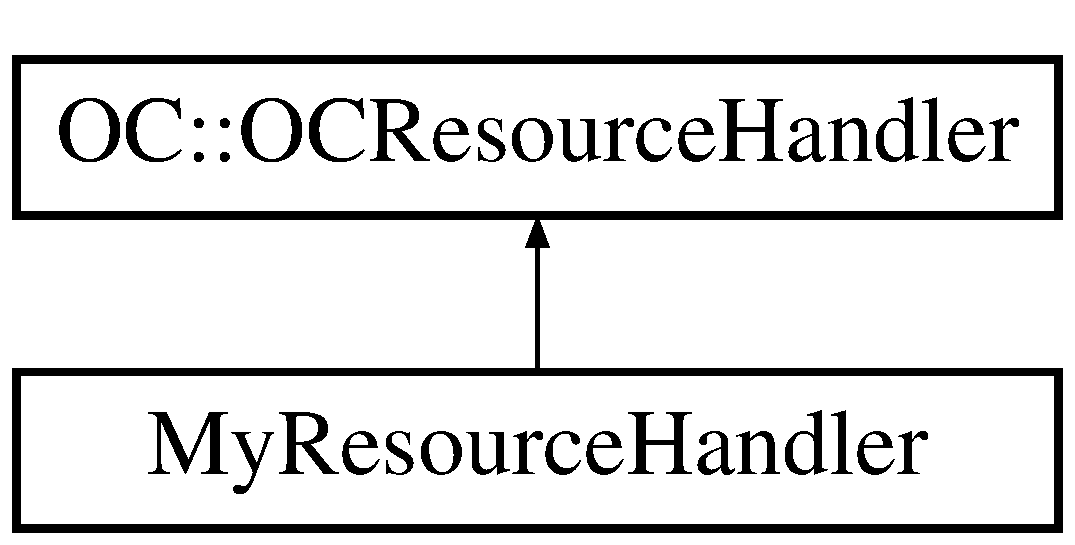
\includegraphics[height=2.000000cm]{classMyResourceHandler}
\end{center}
\end{figure}
\subsection*{Public Member Functions}
\begin{DoxyCompactItemize}
\item 
\hypertarget{classMyResourceHandler_afa8bbbb138a0e1ba0b33d50597c06e24}{}void {\bfseries on\+Found\+Resource} (O\+C\+Resource\+Result $\ast$update, void $\ast$params)\label{classMyResourceHandler_afa8bbbb138a0e1ba0b33d50597c06e24}

\item 
\hypertarget{classMyResourceHandler_ae561787bcebe759437a7a00cc50433a4}{}void {\bfseries on\+Completed} ()\label{classMyResourceHandler_ae561787bcebe759437a7a00cc50433a4}

\item 
\hypertarget{classMyResourceHandler_a3ae345fd8ecd8f3c988187a04788f59f}{}void {\bfseries on\+Failed} ()\label{classMyResourceHandler_a3ae345fd8ecd8f3c988187a04788f59f}

\end{DoxyCompactItemize}


The documentation for this class was generated from the following file\+:\begin{DoxyCompactItemize}
\item 
/home/user/\+O\+I\+C/oic-\/resource/examples/old\+\_\+tests/My\+Resource\+Handler.\+h\end{DoxyCompactItemize}

\hypertarget{structOCCallbackData}{}\section{O\+C\+Callback\+Data Struct Reference}
\label{structOCCallbackData}\index{O\+C\+Callback\+Data@{O\+C\+Callback\+Data}}
\subsection*{Public Attributes}
\begin{DoxyCompactItemize}
\item 
\hypertarget{structOCCallbackData_a21d99e3c61b34603929bb3ccb6d4e4a1}{}void $\ast$ {\bfseries context}\label{structOCCallbackData_a21d99e3c61b34603929bb3ccb6d4e4a1}

\item 
\hypertarget{structOCCallbackData_a77219e4eb938d047a96dd8d9d4a283d7}{}O\+C\+Client\+Response\+Handler {\bfseries cb}\label{structOCCallbackData_a77219e4eb938d047a96dd8d9d4a283d7}

\end{DoxyCompactItemize}


The documentation for this struct was generated from the following file\+:\begin{DoxyCompactItemize}
\item 
/home/user/\+O\+I\+C/oic-\/resource/csdk/stack/include/ocstack.\+h\end{DoxyCompactItemize}

\hypertarget{structOCClientResponse}{}\section{O\+C\+Client\+Response Struct Reference}
\label{structOCClientResponse}\index{O\+C\+Client\+Response@{O\+C\+Client\+Response}}


{\ttfamily \#include $<$ocstack.\+h$>$}

\subsection*{Public Attributes}
\begin{DoxyCompactItemize}
\item 
\hypertarget{structOCClientResponse_a0cdc9f60ffb41713ebe1ea8f3a97f6b6}{}O\+C\+Stack\+Result {\bfseries result}\label{structOCClientResponse_a0cdc9f60ffb41713ebe1ea8f3a97f6b6}

\item 
\hypertarget{structOCClientResponse_ae76c5fded14e466ae1cbaf7f93f8aca2}{}\hyperlink{structOCDevAddr}{O\+C\+Dev\+Addr} $\ast$ {\bfseries addr}\label{structOCClientResponse_ae76c5fded14e466ae1cbaf7f93f8aca2}

\item 
\hypertarget{structOCClientResponse_a6abb39648a7112b78ffd3ab90546e6c4}{}uint32\+\_\+t {\bfseries sequence\+Number}\label{structOCClientResponse_a6abb39648a7112b78ffd3ab90546e6c4}

\item 
\hypertarget{structOCClientResponse_a224ddcb17c24560c66122e2e2a32a153}{}unsigned const char $\ast$ {\bfseries res\+J\+S\+O\+N\+Payload}\label{structOCClientResponse_a224ddcb17c24560c66122e2e2a32a153}

\end{DoxyCompactItemize}


\subsection{Detailed Description}
Response from queries to remote servers. Queries are made by calling the O\+C\+Do\+Resource A\+P\+I. 

The documentation for this struct was generated from the following file\+:\begin{DoxyCompactItemize}
\item 
/home/user/\+O\+I\+C/oic-\/resource/csdk/stack/include/ocstack.\+h\end{DoxyCompactItemize}

\hypertarget{structOCCoAPToken}{}\section{O\+C\+Co\+A\+P\+Token Struct Reference}
\label{structOCCoAPToken}\index{O\+C\+Co\+A\+P\+Token@{O\+C\+Co\+A\+P\+Token}}
\subsection*{Public Attributes}
\begin{DoxyCompactItemize}
\item 
\hypertarget{structOCCoAPToken_a4865c6acfd4790ffc42243ad2351d622}{}uint8\+\_\+t {\bfseries token} \mbox{[}M\+A\+X\+\_\+\+T\+O\+K\+E\+N\+\_\+\+L\+E\+N\+G\+T\+H\mbox{]}\label{structOCCoAPToken_a4865c6acfd4790ffc42243ad2351d622}

\item 
\hypertarget{structOCCoAPToken_a31bca1c8ec03abd13f8984a101e72b64}{}size\+\_\+t {\bfseries token\+Length}\label{structOCCoAPToken_a31bca1c8ec03abd13f8984a101e72b64}

\end{DoxyCompactItemize}


The documentation for this struct was generated from the following file\+:\begin{DoxyCompactItemize}
\item 
/home/user/\+O\+I\+C/oic-\/resource/csdk/occoap/include/occoaptoken.\+h\end{DoxyCompactItemize}

\hypertarget{structOCDevAddr}{}\section{O\+C\+Dev\+Addr Struct Reference}
\label{structOCDevAddr}\index{O\+C\+Dev\+Addr@{O\+C\+Dev\+Addr}}


{\ttfamily \#include $<$ocsocket.\+h$>$}

\subsection*{Public Attributes}
\begin{DoxyCompactItemize}
\item 
uint32\+\_\+t \hyperlink{structOCDevAddr_a491e796c83923aacb93ac5bc8c31325c}{size}
\item 
uint8\+\_\+t \hyperlink{structOCDevAddr_a8d1419ae05d56b162333fdcbac9a6f31}{addr} \mbox{[}D\+E\+V\+\_\+\+A\+D\+D\+R\+\_\+\+S\+I\+Z\+E\+\_\+\+M\+A\+X\mbox{]}
\end{DoxyCompactItemize}


\subsection{Detailed Description}
Data structure to encapsulate I\+Pv4/\+I\+Pv6/\+Contiki/lw\+I\+P device addresses 

\subsection{Member Data Documentation}
\hypertarget{structOCDevAddr_a8d1419ae05d56b162333fdcbac9a6f31}{}\index{O\+C\+Dev\+Addr@{O\+C\+Dev\+Addr}!addr@{addr}}
\index{addr@{addr}!O\+C\+Dev\+Addr@{O\+C\+Dev\+Addr}}
\subsubsection[{addr}]{\setlength{\rightskip}{0pt plus 5cm}uint8\+\_\+t O\+C\+Dev\+Addr\+::addr\mbox{[}D\+E\+V\+\_\+\+A\+D\+D\+R\+\_\+\+S\+I\+Z\+E\+\_\+\+M\+A\+X\mbox{]}}\label{structOCDevAddr_a8d1419ae05d56b162333fdcbac9a6f31}
device address. \hypertarget{structOCDevAddr_a491e796c83923aacb93ac5bc8c31325c}{}\index{O\+C\+Dev\+Addr@{O\+C\+Dev\+Addr}!size@{size}}
\index{size@{size}!O\+C\+Dev\+Addr@{O\+C\+Dev\+Addr}}
\subsubsection[{size}]{\setlength{\rightskip}{0pt plus 5cm}uint32\+\_\+t O\+C\+Dev\+Addr\+::size}\label{structOCDevAddr_a491e796c83923aacb93ac5bc8c31325c}
length of the address stored in addr field. 

The documentation for this struct was generated from the following file\+:\begin{DoxyCompactItemize}
\item 
/home/user/\+O\+I\+C/oic-\/resource/csdk/ocsocket/include/ocsocket.\+h\end{DoxyCompactItemize}

\hypertarget{classoc_1_1ub_1_1OCDiscoverServicesResult}{}\section{oc\+:\+:ub\+:\+:O\+C\+Discover\+Services\+Result Class Reference}
\label{classoc_1_1ub_1_1OCDiscoverServicesResult}\index{oc\+::ub\+::\+O\+C\+Discover\+Services\+Result@{oc\+::ub\+::\+O\+C\+Discover\+Services\+Result}}
\subsection*{Public Member Functions}
\begin{DoxyCompactItemize}
\item 
\hypertarget{classoc_1_1ub_1_1OCDiscoverServicesResult_ac5c60333aecd36c14fc13c82600de3ef}{}virtual O\+C\+Query\+Result\+Type {\bfseries get\+Result} () const =0\label{classoc_1_1ub_1_1OCDiscoverServicesResult_ac5c60333aecd36c14fc13c82600de3ef}

\item 
\hypertarget{classoc_1_1ub_1_1OCDiscoverServicesResult_a5cf0b08937a9a7c96b64d4ee281abf6d}{}virtual const std\+::list$<$ std\+::string $>$ \& {\bfseries get\+Service\+List} () const =0\label{classoc_1_1ub_1_1OCDiscoverServicesResult_a5cf0b08937a9a7c96b64d4ee281abf6d}

\end{DoxyCompactItemize}


The documentation for this class was generated from the following file\+:\begin{DoxyCompactItemize}
\item 
/home/user/\+O\+I\+C/oic-\/resource/csdk/ubstack/include/ocinternalapi.\+h\end{DoxyCompactItemize}

\hypertarget{structOCEntityHandlerRequest}{}\section{O\+C\+Entity\+Handler\+Request Struct Reference}
\label{structOCEntityHandlerRequest}\index{O\+C\+Entity\+Handler\+Request@{O\+C\+Entity\+Handler\+Request}}


The O\+C\+Entity\+Handler callback A\+P\+I must be implemented in the application in order to receive these requests.  




{\ttfamily \#include $<$ocstack.\+h$>$}

\subsection*{Public Attributes}
\begin{DoxyCompactItemize}
\item 
\hypertarget{structOCEntityHandlerRequest_abf4e21b81325371446fc248f506f35f5}{}O\+C\+Resource\+Handle {\bfseries resource}\label{structOCEntityHandlerRequest_abf4e21b81325371446fc248f506f35f5}

\item 
\hypertarget{structOCEntityHandlerRequest_a966c2fd243671760bb918911db36b05e}{}unsigned char $\ast$ {\bfseries query}\label{structOCEntityHandlerRequest_a966c2fd243671760bb918911db36b05e}

\item 
\hypertarget{structOCEntityHandlerRequest_a1d2ff6d9f125ed7ef6c6db64d939f601}{}O\+C\+Method {\bfseries method}\label{structOCEntityHandlerRequest_a1d2ff6d9f125ed7ef6c6db64d939f601}

\item 
\hypertarget{structOCEntityHandlerRequest_a67f5f8e7ac44c4fd89c3b45d1e8a583b}{}unsigned const char $\ast$ {\bfseries req\+J\+S\+O\+N\+Payload}\label{structOCEntityHandlerRequest_a67f5f8e7ac44c4fd89c3b45d1e8a583b}

\item 
\hypertarget{structOCEntityHandlerRequest_a568bf6be5ad919ff1ef6fb90988ff34f}{}unsigned char $\ast$ {\bfseries res\+J\+S\+O\+N\+Payload}\label{structOCEntityHandlerRequest_a568bf6be5ad919ff1ef6fb90988ff34f}

\item 
\hypertarget{structOCEntityHandlerRequest_a491cd26225419fe6494f11be0917236c}{}uint16\+\_\+t {\bfseries res\+J\+S\+O\+N\+Payload\+Len}\label{structOCEntityHandlerRequest_a491cd26225419fe6494f11be0917236c}

\end{DoxyCompactItemize}


\subsection{Detailed Description}
The O\+C\+Entity\+Handler callback A\+P\+I must be implemented in the application in order to receive these requests. 

Incoming requests handled by the server. Requests are passed in as a parameter to the O\+C\+Entity\+Handler callback A\+P\+I. 

The documentation for this struct was generated from the following file\+:\begin{DoxyCompactItemize}
\item 
/home/user/\+O\+I\+C/oic-\/resource/csdk/stack/include/ocstack.\+h\end{DoxyCompactItemize}

\hypertarget{classOC_1_1OCException}{}\section{O\+C\+:\+:O\+C\+Exception Class Reference}
\label{classOC_1_1OCException}\index{O\+C\+::\+O\+C\+Exception@{O\+C\+::\+O\+C\+Exception}}
Inheritance diagram for O\+C\+:\+:O\+C\+Exception\+:\begin{figure}[H]
\begin{center}
\leavevmode
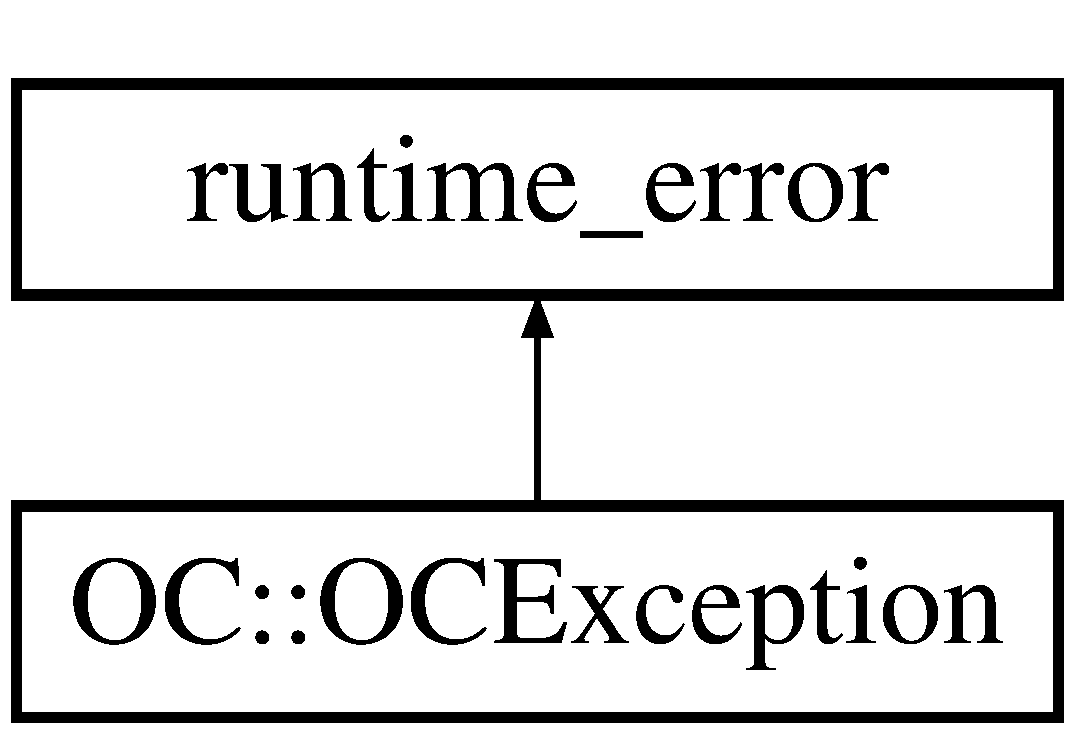
\includegraphics[height=2.000000cm]{classOC_1_1OCException}
\end{center}
\end{figure}
\subsection*{Public Member Functions}
\begin{DoxyCompactItemize}
\item 
\hypertarget{classOC_1_1OCException_a88300c0e6db05f0392431cd04a0d1eba}{}{\bfseries O\+C\+Exception} (const std\+::string \&msg, O\+C\+Stack\+Result reason=O\+C\+\_\+\+S\+T\+A\+C\+K\+\_\+\+E\+R\+R\+O\+R)\label{classOC_1_1OCException_a88300c0e6db05f0392431cd04a0d1eba}

\item 
\hypertarget{classOC_1_1OCException_a41a455855fd902af894914ded12c7c03}{}std\+::string {\bfseries reason} ()\label{classOC_1_1OCException_a41a455855fd902af894914ded12c7c03}

\end{DoxyCompactItemize}


The documentation for this class was generated from the following file\+:\begin{DoxyCompactItemize}
\item 
/home/user/\+O\+I\+C/oic-\/resource/include/O\+C\+Exception.\+h\end{DoxyCompactItemize}

\hypertarget{classoc_1_1ub_1_1OCModel}{}\section{oc\+:\+:ub\+:\+:O\+C\+Model Class Reference}
\label{classoc_1_1ub_1_1OCModel}\index{oc\+::ub\+::\+O\+C\+Model@{oc\+::ub\+::\+O\+C\+Model}}
Inheritance diagram for oc\+:\+:ub\+:\+:O\+C\+Model\+:\begin{figure}[H]
\begin{center}
\leavevmode
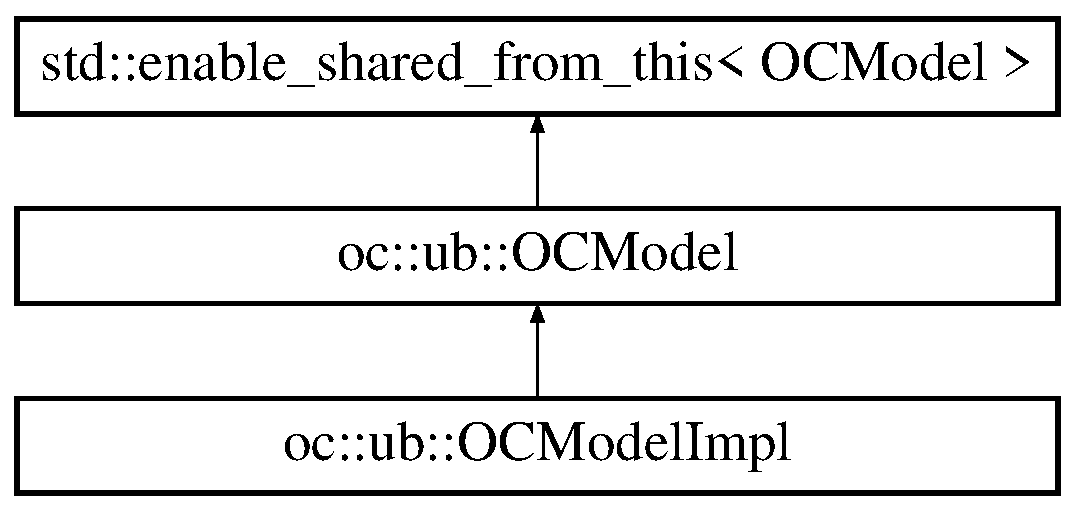
\includegraphics[height=3.000000cm]{classoc_1_1ub_1_1OCModel}
\end{center}
\end{figure}
\subsection*{Public Types}
\begin{DoxyCompactItemize}
\item 
\hypertarget{classoc_1_1ub_1_1OCModel_a41a06fcd1b57bb031e7348e9f40681b1}{}typedef std\+::shared\+\_\+ptr$<$ \hyperlink{classoc_1_1ub_1_1OCModel}{O\+C\+Model} $>$ {\bfseries Shared\+Ptr}\label{classoc_1_1ub_1_1OCModel_a41a06fcd1b57bb031e7348e9f40681b1}

\item 
\hypertarget{classoc_1_1ub_1_1OCModel_ace13bbe5a684c5b01a294912fa656e5d}{}typedef std\+::weak\+\_\+ptr$<$ \hyperlink{classoc_1_1ub_1_1OCModel}{O\+C\+Model} $>$ {\bfseries Weak\+Ptr}\label{classoc_1_1ub_1_1OCModel_ace13bbe5a684c5b01a294912fa656e5d}

\end{DoxyCompactItemize}
\subsection*{Public Member Functions}
\begin{DoxyCompactItemize}
\item 
virtual bool \hyperlink{classoc_1_1ub_1_1OCModel_ae9c3633d98ea85798de3c35f87a1e09c}{start} (const std\+::string ip\+Addr, int16\+\_\+t port, O\+C\+Stack\+Mode mode)=0
\item 
virtual void \hyperlink{classoc_1_1ub_1_1OCModel_a415bb23e3d0cb7c0ff08166d46fd660b}{discover\+Services} (O\+C\+Discover\+Services\+Function \&async\+Return\+Func)=0
\item 
virtual uint16\+\_\+t \hyperlink{classoc_1_1ub_1_1OCModel_aa11c34b45df6a00aad454cb23a72ec6f}{add\+Service} (const std\+::string url)=0
\end{DoxyCompactItemize}
\subsection*{Static Public Member Functions}
\begin{DoxyCompactItemize}
\item 
\hypertarget{classoc_1_1ub_1_1OCModel_a0fb2eb25864e3d08b561a65e0e1e01cd}{}static Shared\+Ptr {\bfseries create\+Model} ()\label{classoc_1_1ub_1_1OCModel_a0fb2eb25864e3d08b561a65e0e1e01cd}

\end{DoxyCompactItemize}


\subsection{Member Function Documentation}
\hypertarget{classoc_1_1ub_1_1OCModel_aa11c34b45df6a00aad454cb23a72ec6f}{}\index{oc\+::ub\+::\+O\+C\+Model@{oc\+::ub\+::\+O\+C\+Model}!add\+Service@{add\+Service}}
\index{add\+Service@{add\+Service}!oc\+::ub\+::\+O\+C\+Model@{oc\+::ub\+::\+O\+C\+Model}}
\subsubsection[{add\+Service}]{\setlength{\rightskip}{0pt plus 5cm}virtual uint16\+\_\+t oc\+::ub\+::\+O\+C\+Model\+::add\+Service (
\begin{DoxyParamCaption}
\item[{const std\+::string}]{url}
\end{DoxyParamCaption}
)\hspace{0.3cm}{\ttfamily [pure virtual]}}\label{classoc_1_1ub_1_1OCModel_aa11c34b45df6a00aad454cb23a72ec6f}
Add a service to the \hyperlink{classoc_1_1ub_1_1OCModel}{O\+C\+Model}


\begin{DoxyParams}{Parameters}
{\em url} & U\+R\+L of the service\\
\hline
\end{DoxyParams}
\begin{DoxyReturn}{Returns}
Total number of services in the \hyperlink{classoc_1_1ub_1_1OCModel}{O\+C\+Model} 
\end{DoxyReturn}


Implemented in \hyperlink{classoc_1_1ub_1_1OCModelImpl_af4266972dedd3e3e3955f57795692d63}{oc\+::ub\+::\+O\+C\+Model\+Impl}.

\hypertarget{classoc_1_1ub_1_1OCModel_a415bb23e3d0cb7c0ff08166d46fd660b}{}\index{oc\+::ub\+::\+O\+C\+Model@{oc\+::ub\+::\+O\+C\+Model}!discover\+Services@{discover\+Services}}
\index{discover\+Services@{discover\+Services}!oc\+::ub\+::\+O\+C\+Model@{oc\+::ub\+::\+O\+C\+Model}}
\subsubsection[{discover\+Services}]{\setlength{\rightskip}{0pt plus 5cm}virtual void oc\+::ub\+::\+O\+C\+Model\+::discover\+Services (
\begin{DoxyParamCaption}
\item[{O\+C\+Discover\+Services\+Function \&}]{async\+Return\+Func}
\end{DoxyParamCaption}
)\hspace{0.3cm}{\ttfamily [pure virtual]}}\label{classoc_1_1ub_1_1OCModel_a415bb23e3d0cb7c0ff08166d46fd660b}
Get all services that have been discovered at time of call


\begin{DoxyParams}{Parameters}
{\em async\+Return\+Func} & -\/ asynchronous callback function that is invoked by the \hyperlink{classoc_1_1ub_1_1OCModel}{O\+C\+Model} when service discovery is complete. The callback will include status and a list of all discovered services \\
\hline
\end{DoxyParams}


Implemented in \hyperlink{classoc_1_1ub_1_1OCModelImpl_a246179adaa5c8cd2288ef80f85a940dd}{oc\+::ub\+::\+O\+C\+Model\+Impl}.

\hypertarget{classoc_1_1ub_1_1OCModel_ae9c3633d98ea85798de3c35f87a1e09c}{}\index{oc\+::ub\+::\+O\+C\+Model@{oc\+::ub\+::\+O\+C\+Model}!start@{start}}
\index{start@{start}!oc\+::ub\+::\+O\+C\+Model@{oc\+::ub\+::\+O\+C\+Model}}
\subsubsection[{start}]{\setlength{\rightskip}{0pt plus 5cm}virtual bool oc\+::ub\+::\+O\+C\+Model\+::start (
\begin{DoxyParamCaption}
\item[{const std\+::string}]{ip\+Addr, }
\item[{int16\+\_\+t}]{port, }
\item[{O\+C\+Stack\+Mode}]{mode}
\end{DoxyParamCaption}
)\hspace{0.3cm}{\ttfamily [pure virtual]}}\label{classoc_1_1ub_1_1OCModel_ae9c3633d98ea85798de3c35f87a1e09c}
Start the \hyperlink{namespaceOC}{O\+C} Stack.


\begin{DoxyParams}{Parameters}
{\em ip\+Addr} & I\+P Address of host device \\
\hline
{\em port} & Port of host device \\
\hline
{\em mode} & Host device is client, server, or client-\/server\\
\hline
\end{DoxyParams}
\begin{DoxyReturn}{Returns}
true -\/ successfully started the \hyperlink{namespaceOC}{O\+C} Stack false -\/ error starting the \hyperlink{namespaceOC}{O\+C} Stack 
\end{DoxyReturn}


Implemented in \hyperlink{classoc_1_1ub_1_1OCModelImpl_a7c6ce055a165c371b1d193464510d94b}{oc\+::ub\+::\+O\+C\+Model\+Impl}.



The documentation for this class was generated from the following file\+:\begin{DoxyCompactItemize}
\item 
/home/user/\+O\+I\+C/oic-\/resource/csdk/ubstack/include/ocinternalapi.\+h\end{DoxyCompactItemize}

\hypertarget{classoc_1_1ub_1_1OCModelImpl}{}\section{oc\+:\+:ub\+:\+:O\+C\+Model\+Impl Class Reference}
\label{classoc_1_1ub_1_1OCModelImpl}\index{oc\+::ub\+::\+O\+C\+Model\+Impl@{oc\+::ub\+::\+O\+C\+Model\+Impl}}
Inheritance diagram for oc\+:\+:ub\+:\+:O\+C\+Model\+Impl\+:\begin{figure}[H]
\begin{center}
\leavevmode
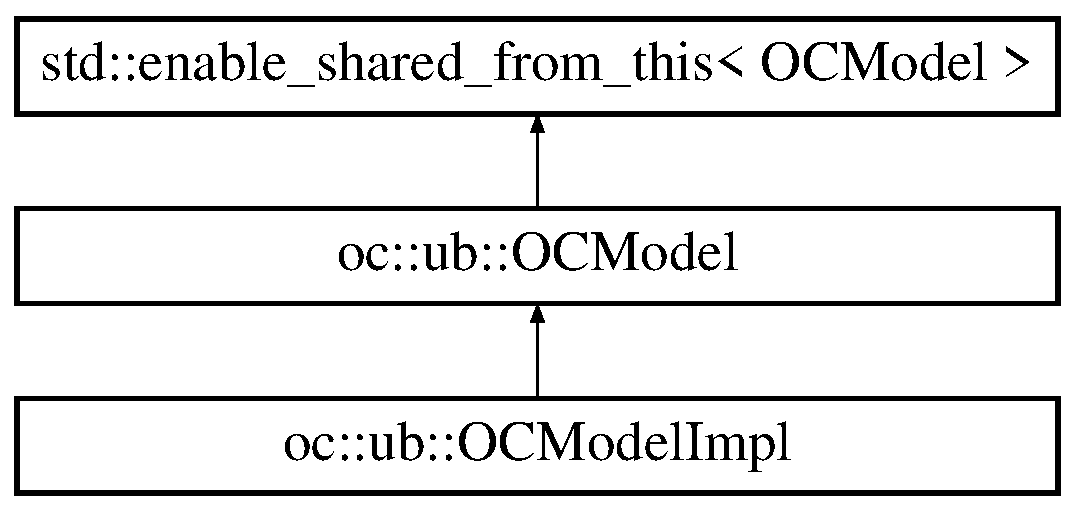
\includegraphics[height=3.000000cm]{classoc_1_1ub_1_1OCModelImpl}
\end{center}
\end{figure}
\subsection*{Public Types}
\begin{DoxyCompactItemize}
\item 
\hypertarget{classoc_1_1ub_1_1OCModelImpl_a5b323ffe75d8614854b0aa8b83fdf0e4}{}typedef std\+::shared\+\_\+ptr$<$ \hyperlink{classoc_1_1ub_1_1OCModelImpl}{O\+C\+Model\+Impl} $>$ {\bfseries Shared\+Ptr}\label{classoc_1_1ub_1_1OCModelImpl_a5b323ffe75d8614854b0aa8b83fdf0e4}

\item 
\hypertarget{classoc_1_1ub_1_1OCModelImpl_a0b39ccd354aa7b2b521cba85b87948e4}{}typedef std\+::weak\+\_\+ptr$<$ \hyperlink{classoc_1_1ub_1_1OCModelImpl}{O\+C\+Model\+Impl} $>$ {\bfseries Weak\+Ptr}\label{classoc_1_1ub_1_1OCModelImpl_a0b39ccd354aa7b2b521cba85b87948e4}

\end{DoxyCompactItemize}
\subsection*{Public Member Functions}
\begin{DoxyCompactItemize}
\item 
\hyperlink{classoc_1_1ub_1_1OCModelImpl_ab30a99e6992ef75e5dd604507c0e4c69}{O\+C\+Model\+Impl} ()
\item 
virtual \hyperlink{classoc_1_1ub_1_1OCModelImpl_a116c96f3e9c1daa9d82608b4420ae7ff}{$\sim$\+O\+C\+Model\+Impl} ()
\item 
virtual bool \hyperlink{classoc_1_1ub_1_1OCModelImpl_a7c6ce055a165c371b1d193464510d94b}{start} (const std\+::string ip\+Addr, int16\+\_\+t port, O\+C\+Stack\+Mode mode)
\item 
virtual void \hyperlink{classoc_1_1ub_1_1OCModelImpl_a246179adaa5c8cd2288ef80f85a940dd}{discover\+Services} (O\+C\+Discover\+Services\+Function \&async\+Return\+Func)
\item 
virtual uint16\+\_\+t \hyperlink{classoc_1_1ub_1_1OCModelImpl_af4266972dedd3e3e3955f57795692d63}{add\+Service} (const std\+::string url)
\end{DoxyCompactItemize}
\subsection*{Static Public Member Functions}
\begin{DoxyCompactItemize}
\item 
static Shared\+Ptr \hyperlink{classoc_1_1ub_1_1OCModelImpl_a5097d6ac72eee4a7f0d9c1aac9f5fb5e}{create\+Model} ()
\end{DoxyCompactItemize}
\subsection*{Friends}
\begin{DoxyCompactItemize}
\item 
void \hyperlink{classoc_1_1ub_1_1OCModelImpl_a3f81e802eb9c5d3c901a4dca02dee6a3}{async\+Do\+Resources\+Callback} (O\+C\+Stack\+Result result, O\+C\+Representation\+Handle representation)
\end{DoxyCompactItemize}


\subsection{Constructor \& Destructor Documentation}
\hypertarget{classoc_1_1ub_1_1OCModelImpl_ab30a99e6992ef75e5dd604507c0e4c69}{}\index{oc\+::ub\+::\+O\+C\+Model\+Impl@{oc\+::ub\+::\+O\+C\+Model\+Impl}!O\+C\+Model\+Impl@{O\+C\+Model\+Impl}}
\index{O\+C\+Model\+Impl@{O\+C\+Model\+Impl}!oc\+::ub\+::\+O\+C\+Model\+Impl@{oc\+::ub\+::\+O\+C\+Model\+Impl}}
\subsubsection[{O\+C\+Model\+Impl}]{\setlength{\rightskip}{0pt plus 5cm}oc\+::ub\+::\+O\+C\+Model\+Impl\+::\+O\+C\+Model\+Impl (
\begin{DoxyParamCaption}
{}
\end{DoxyParamCaption}
)}\label{classoc_1_1ub_1_1OCModelImpl_ab30a99e6992ef75e5dd604507c0e4c69}
Constructor \hypertarget{classoc_1_1ub_1_1OCModelImpl_a116c96f3e9c1daa9d82608b4420ae7ff}{}\index{oc\+::ub\+::\+O\+C\+Model\+Impl@{oc\+::ub\+::\+O\+C\+Model\+Impl}!````~O\+C\+Model\+Impl@{$\sim$\+O\+C\+Model\+Impl}}
\index{````~O\+C\+Model\+Impl@{$\sim$\+O\+C\+Model\+Impl}!oc\+::ub\+::\+O\+C\+Model\+Impl@{oc\+::ub\+::\+O\+C\+Model\+Impl}}
\subsubsection[{$\sim$\+O\+C\+Model\+Impl}]{\setlength{\rightskip}{0pt plus 5cm}virtual oc\+::ub\+::\+O\+C\+Model\+Impl\+::$\sim$\+O\+C\+Model\+Impl (
\begin{DoxyParamCaption}
{}
\end{DoxyParamCaption}
)\hspace{0.3cm}{\ttfamily [virtual]}}\label{classoc_1_1ub_1_1OCModelImpl_a116c96f3e9c1daa9d82608b4420ae7ff}
Destructor 

\subsection{Member Function Documentation}
\hypertarget{classoc_1_1ub_1_1OCModelImpl_af4266972dedd3e3e3955f57795692d63}{}\index{oc\+::ub\+::\+O\+C\+Model\+Impl@{oc\+::ub\+::\+O\+C\+Model\+Impl}!add\+Service@{add\+Service}}
\index{add\+Service@{add\+Service}!oc\+::ub\+::\+O\+C\+Model\+Impl@{oc\+::ub\+::\+O\+C\+Model\+Impl}}
\subsubsection[{add\+Service}]{\setlength{\rightskip}{0pt plus 5cm}virtual uint16\+\_\+t oc\+::ub\+::\+O\+C\+Model\+Impl\+::add\+Service (
\begin{DoxyParamCaption}
\item[{const std\+::string}]{url}
\end{DoxyParamCaption}
)\hspace{0.3cm}{\ttfamily [virtual]}}\label{classoc_1_1ub_1_1OCModelImpl_af4266972dedd3e3e3955f57795692d63}
Add a service to the \hyperlink{classoc_1_1ub_1_1OCModelImpl}{O\+C\+Model\+Impl}


\begin{DoxyParams}{Parameters}
{\em url} & -\/ U\+R\+L of the service \\
\hline
\end{DoxyParams}
\begin{DoxyReturn}{Returns}
Total number of services in the \hyperlink{classoc_1_1ub_1_1OCModelImpl}{O\+C\+Model\+Impl} 
\end{DoxyReturn}


Implements \hyperlink{classoc_1_1ub_1_1OCModel_aa11c34b45df6a00aad454cb23a72ec6f}{oc\+::ub\+::\+O\+C\+Model}.

\hypertarget{classoc_1_1ub_1_1OCModelImpl_a5097d6ac72eee4a7f0d9c1aac9f5fb5e}{}\index{oc\+::ub\+::\+O\+C\+Model\+Impl@{oc\+::ub\+::\+O\+C\+Model\+Impl}!create\+Model@{create\+Model}}
\index{create\+Model@{create\+Model}!oc\+::ub\+::\+O\+C\+Model\+Impl@{oc\+::ub\+::\+O\+C\+Model\+Impl}}
\subsubsection[{create\+Model}]{\setlength{\rightskip}{0pt plus 5cm}static Shared\+Ptr oc\+::ub\+::\+O\+C\+Model\+Impl\+::create\+Model (
\begin{DoxyParamCaption}
{}
\end{DoxyParamCaption}
)\hspace{0.3cm}{\ttfamily [static]}}\label{classoc_1_1ub_1_1OCModelImpl_a5097d6ac72eee4a7f0d9c1aac9f5fb5e}
Factory pattern to create a \hyperlink{classoc_1_1ub_1_1OCModel}{O\+C\+Model} singleton \begin{DoxyReturn}{Returns}
Shared pointer to the \hyperlink{classoc_1_1ub_1_1OCModel}{O\+C\+Model} 
\end{DoxyReturn}
\hypertarget{classoc_1_1ub_1_1OCModelImpl_a246179adaa5c8cd2288ef80f85a940dd}{}\index{oc\+::ub\+::\+O\+C\+Model\+Impl@{oc\+::ub\+::\+O\+C\+Model\+Impl}!discover\+Services@{discover\+Services}}
\index{discover\+Services@{discover\+Services}!oc\+::ub\+::\+O\+C\+Model\+Impl@{oc\+::ub\+::\+O\+C\+Model\+Impl}}
\subsubsection[{discover\+Services}]{\setlength{\rightskip}{0pt plus 5cm}virtual void oc\+::ub\+::\+O\+C\+Model\+Impl\+::discover\+Services (
\begin{DoxyParamCaption}
\item[{O\+C\+Discover\+Services\+Function \&}]{async\+Return\+Func}
\end{DoxyParamCaption}
)\hspace{0.3cm}{\ttfamily [virtual]}}\label{classoc_1_1ub_1_1OCModelImpl_a246179adaa5c8cd2288ef80f85a940dd}
Get all services that have been discovered at time of call


\begin{DoxyParams}{Parameters}
{\em async\+Return\+Func} & -\/ asynchronous callback function that is invoked by the \hyperlink{classoc_1_1ub_1_1OCModelImpl}{O\+C\+Model\+Impl} when service discovery is complete. The callback will include status and a list of all discovered services \\
\hline
\end{DoxyParams}


Implements \hyperlink{classoc_1_1ub_1_1OCModel_a415bb23e3d0cb7c0ff08166d46fd660b}{oc\+::ub\+::\+O\+C\+Model}.

\hypertarget{classoc_1_1ub_1_1OCModelImpl_a7c6ce055a165c371b1d193464510d94b}{}\index{oc\+::ub\+::\+O\+C\+Model\+Impl@{oc\+::ub\+::\+O\+C\+Model\+Impl}!start@{start}}
\index{start@{start}!oc\+::ub\+::\+O\+C\+Model\+Impl@{oc\+::ub\+::\+O\+C\+Model\+Impl}}
\subsubsection[{start}]{\setlength{\rightskip}{0pt plus 5cm}virtual bool oc\+::ub\+::\+O\+C\+Model\+Impl\+::start (
\begin{DoxyParamCaption}
\item[{const std\+::string}]{ip\+Addr, }
\item[{int16\+\_\+t}]{port, }
\item[{O\+C\+Stack\+Mode}]{mode}
\end{DoxyParamCaption}
)\hspace{0.3cm}{\ttfamily [virtual]}}\label{classoc_1_1ub_1_1OCModelImpl_a7c6ce055a165c371b1d193464510d94b}
Start the \hyperlink{namespaceOC}{O\+C} Stack.


\begin{DoxyParams}{Parameters}
{\em ip\+Addr} & I\+P Address of host device \\
\hline
{\em port} & Port of host device$\ast$ \\
\hline
{\em mode} & Host device is client, server, or client-\/server\\
\hline
\end{DoxyParams}
\begin{DoxyReturn}{Returns}
true -\/ successfully started the \hyperlink{namespaceOC}{O\+C} Stack false -\/ error starting the \hyperlink{namespaceOC}{O\+C} Stack 
\end{DoxyReturn}


Implements \hyperlink{classoc_1_1ub_1_1OCModel_ae9c3633d98ea85798de3c35f87a1e09c}{oc\+::ub\+::\+O\+C\+Model}.



\subsection{Friends And Related Function Documentation}
\hypertarget{classoc_1_1ub_1_1OCModelImpl_a3f81e802eb9c5d3c901a4dca02dee6a3}{}\index{oc\+::ub\+::\+O\+C\+Model\+Impl@{oc\+::ub\+::\+O\+C\+Model\+Impl}!async\+Do\+Resources\+Callback@{async\+Do\+Resources\+Callback}}
\index{async\+Do\+Resources\+Callback@{async\+Do\+Resources\+Callback}!oc\+::ub\+::\+O\+C\+Model\+Impl@{oc\+::ub\+::\+O\+C\+Model\+Impl}}
\subsubsection[{async\+Do\+Resources\+Callback}]{\setlength{\rightskip}{0pt plus 5cm}void async\+Do\+Resources\+Callback (
\begin{DoxyParamCaption}
\item[{O\+C\+Stack\+Result}]{result, }
\item[{O\+C\+Representation\+Handle}]{representation}
\end{DoxyParamCaption}
)\hspace{0.3cm}{\ttfamily [friend]}}\label{classoc_1_1ub_1_1OCModelImpl_a3f81e802eb9c5d3c901a4dca02dee6a3}
Asynchronous callback friend function invoked by the \hyperlink{namespaceOC}{O\+C} Stack upon service discovery


\begin{DoxyParams}{Parameters}
{\em result} & -\/ \hyperlink{namespaceOC}{O\+C} stack result \\
\hline
{\em representation} & -\/ handle to the representation of the resource \\
\hline
\end{DoxyParams}


The documentation for this class was generated from the following file\+:\begin{DoxyCompactItemize}
\item 
/home/user/\+O\+I\+C/oic-\/resource/csdk/ubstack/src/ocmodelimpl.\+h\end{DoxyCompactItemize}

\hypertarget{classOC_1_1OCObject}{}\section{O\+C\+:\+:O\+C\+Object Class Reference}
\label{classOC_1_1OCObject}\index{O\+C\+::\+O\+C\+Object@{O\+C\+::\+O\+C\+Object}}


The \hyperlink{classOC_1_1OCObject}{O\+C\+Object} is the root abstract class from which many of the \hyperlink{namespaceOC}{O\+C} related objects derive from. It implements a common set of functionality supported by all the \hyperlink{namespaceOC}{O\+C} classes in the S\+D\+K such as object naming, I\+D, natural sort order and comparison.  




{\ttfamily \#include $<$O\+C\+Object.\+h$>$}

\subsection*{Public Member Functions}
\begin{DoxyCompactItemize}
\item 
\hypertarget{classOC_1_1OCObject_a67e15b0b14e4744665c75f1e1824eb08}{}virtual bool {\bfseries is\+Visible} ()=0\label{classOC_1_1OCObject_a67e15b0b14e4744665c75f1e1824eb08}

\end{DoxyCompactItemize}


\subsection{Detailed Description}
The \hyperlink{classOC_1_1OCObject}{O\+C\+Object} is the root abstract class from which many of the \hyperlink{namespaceOC}{O\+C} related objects derive from. It implements a common set of functionality supported by all the \hyperlink{namespaceOC}{O\+C} classes in the S\+D\+K such as object naming, I\+D, natural sort order and comparison. 

The documentation for this class was generated from the following file\+:\begin{DoxyCompactItemize}
\item 
/home/user/\+O\+I\+C/oic-\/resource/include/\hyperlink{OCObject_8h}{O\+C\+Object.\+h}\end{DoxyCompactItemize}

\hypertarget{classOC_1_1OCObserver}{}\section{O\+C\+:\+:O\+C\+Observer Class Reference}
\label{classOC_1_1OCObserver}\index{O\+C\+::\+O\+C\+Observer@{O\+C\+::\+O\+C\+Observer}}


The documentation for this class was generated from the following file\+:\begin{DoxyCompactItemize}
\item 
/home/user/\+O\+I\+C/oic-\/resource/include/\hyperlink{OCObserver_8h}{O\+C\+Observer.\+h}\end{DoxyCompactItemize}

\hypertarget{structOCObserveReq}{}\section{O\+C\+Observe\+Req Struct Reference}
\label{structOCObserveReq}\index{O\+C\+Observe\+Req@{O\+C\+Observe\+Req}}
\subsection*{Public Attributes}
\begin{DoxyCompactItemize}
\item 
\hypertarget{structOCObserveReq_a2be6552e558495c16f70fd085570a088}{}uint8\+\_\+t {\bfseries option}\label{structOCObserveReq_a2be6552e558495c16f70fd085570a088}

\item 
\hypertarget{structOCObserveReq_adf24154476af84f82987273715b5fe92}{}\hyperlink{structOCDevAddr}{O\+C\+Dev\+Addr} $\ast$ {\bfseries sub\+Addr}\label{structOCObserveReq_adf24154476af84f82987273715b5fe92}

\item 
\hypertarget{structOCObserveReq_a54dad1d33411464f8a2769406d7978b2}{}\hyperlink{structOCCoAPToken}{O\+C\+Co\+A\+P\+Token} $\ast$ {\bfseries token}\label{structOCObserveReq_a54dad1d33411464f8a2769406d7978b2}

\item 
\hypertarget{structOCObserveReq_ae8212f08e16b6d604b98aa3647bb22d6}{}O\+C\+Stack\+Result {\bfseries result}\label{structOCObserveReq_ae8212f08e16b6d604b98aa3647bb22d6}

\end{DoxyCompactItemize}


The documentation for this struct was generated from the following file\+:\begin{DoxyCompactItemize}
\item 
/home/user/\+O\+I\+C/oic-\/resource/csdk/stack/include/internal/ocstackinternal.\+h\end{DoxyCompactItemize}

\hypertarget{classOC_1_1OCObserverHandler}{}\section{O\+C\+:\+:O\+C\+Observer\+Handler Class Reference}
\label{classOC_1_1OCObserverHandler}\index{O\+C\+::\+O\+C\+Observer\+Handler@{O\+C\+::\+O\+C\+Observer\+Handler}}


\hyperlink{classOC_1_1OCObserverHandler}{O\+C\+Observer\+Handler} is a pure abstract class and it can be used for observer related callbacks.  




{\ttfamily \#include $<$O\+C\+Observer\+Handler.\+h$>$}

Inheritance diagram for O\+C\+:\+:O\+C\+Observer\+Handler\+:\begin{figure}[H]
\begin{center}
\leavevmode
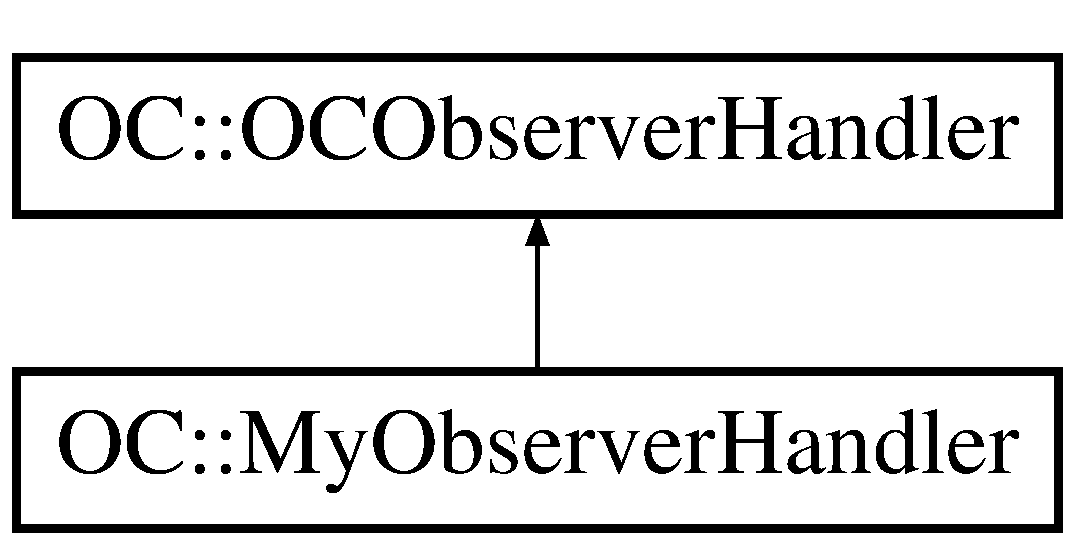
\includegraphics[height=2.000000cm]{classOC_1_1OCObserverHandler}
\end{center}
\end{figure}
\subsection*{Public Member Functions}
\begin{DoxyCompactItemize}
\item 
\hypertarget{classOC_1_1OCObserverHandler_a619e713e6ec000523c3d33b17f2feec0}{}virtual void {\bfseries on\+Observer\+Update} (std\+::string property\+Name, void $\ast$value)=0\label{classOC_1_1OCObserverHandler_a619e713e6ec000523c3d33b17f2feec0}

\end{DoxyCompactItemize}


\subsection{Detailed Description}
\hyperlink{classOC_1_1OCObserverHandler}{O\+C\+Observer\+Handler} is a pure abstract class and it can be used for observer related callbacks. 

The documentation for this class was generated from the following file\+:\begin{DoxyCompactItemize}
\item 
/home/user/\+O\+I\+C/oic-\/resource/include/\hyperlink{OCObserverHandler_8h}{O\+C\+Observer\+Handler.\+h}\end{DoxyCompactItemize}

\hypertarget{classOC_1_1OCPlatform}{}\section{O\+C\+:\+:O\+C\+Platform Class Reference}
\label{classOC_1_1OCPlatform}\index{O\+C\+::\+O\+C\+Platform@{O\+C\+::\+O\+C\+Platform}}


Both server and client must initialize the core platform by instantiating \hyperlink{classOC_1_1OCPlatform}{O\+C\+Platform}. On successful initialization, an instance of the \hyperlink{classOC_1_1OCPlatform}{O\+C\+Platform} is returned. A\+P\+Is in \hyperlink{classOC_1_1OCPlatform}{O\+C\+Platform} provide mechanism to register a resource and host the resource on the server, find resources on the network etc.  




{\ttfamily \#include $<$O\+C\+Platform.\+h$>$}

\subsection*{Public Types}
\begin{DoxyCompactItemize}
\item 
\hypertarget{classOC_1_1OCPlatform_a61eeef7ea8333dd6a6656871748aa6e5}{}typedef O\+C\+Do\+Handle {\bfseries O\+C\+Presence\+Handle}\label{classOC_1_1OCPlatform_a61eeef7ea8333dd6a6656871748aa6e5}

\end{DoxyCompactItemize}
\subsection*{Public Member Functions}
\begin{DoxyCompactItemize}
\item 
\hyperlink{classOC_1_1OCPlatform_a6a8fab4d7a96e6608b0be1312b131580}{O\+C\+Platform} (const \hyperlink{structOC_1_1PlatformConfig}{Platform\+Config} \&config)
\item 
virtual \hyperlink{classOC_1_1OCPlatform_a64a502e9c3efd151ad1e849e8678dcb6}{$\sim$\+O\+C\+Platform} (void)
\item 
O\+C\+Stack\+Result \hyperlink{classOC_1_1OCPlatform_a6c93e271dca1a61f237ebea4c795f208}{find\+Resource} (const std\+::string \&host, const std\+::string \&resource\+U\+R\+I, Find\+Callback resource\+Handler)
\item 
O\+C\+Stack\+Result \hyperlink{classOC_1_1OCPlatform_aa719897291b5e6668f026e2e4b861cab}{register\+Resource} (O\+C\+Resource\+Handle \&resource\+Handle, std\+::string \&resource\+U\+R\+I, const std\+::string \&resource\+Type\+Name, const std\+::string \&resource\+Interface, Register\+Callback entity\+Handler, uint8\+\_\+t resource\+Property)
\item 
O\+C\+Stack\+Result \hyperlink{classOC_1_1OCPlatform_ae42baa45cd2e70062b7582f8bbbdcc9a}{unregister\+Resource} (const O\+C\+Resource\+Handle \&resource\+Handle) const 
\item 
O\+C\+Stack\+Result \hyperlink{classOC_1_1OCPlatform_ac4594ddc58963001de33bff8072ff22f}{bind\+Resource} (const O\+C\+Resource\+Handle collection\+Handle, const O\+C\+Resource\+Handle resource\+Handle)
\item 
O\+C\+Stack\+Result \hyperlink{classOC_1_1OCPlatform_a59c5b855f03c7cdd89d64bd162978bd0}{bind\+Resources} (const O\+C\+Resource\+Handle collection\+Handle, const std\+::vector$<$ O\+C\+Resource\+Handle $>$ \&added\+Resource\+Handle\+List)
\item 
O\+C\+Stack\+Result \hyperlink{classOC_1_1OCPlatform_af5c0276b46cffef81efeb2738fb1bd98}{unbind\+Resource} (const O\+C\+Resource\+Handle collection\+Handle, const O\+C\+Resource\+Handle resource\+Handle)
\item 
O\+C\+Stack\+Result \hyperlink{classOC_1_1OCPlatform_ab292d40d546e7e5d6df1274237399dfc}{unbind\+Resources} (const O\+C\+Resource\+Handle collection\+Handle, const std\+::vector$<$ O\+C\+Resource\+Handle $>$ \&resource\+Handle\+List)
\item 
O\+C\+Stack\+Result \hyperlink{classOC_1_1OCPlatform_a3a7f2658df5b17be3641dd3646aa5af8}{bind\+Type\+To\+Resource} (const O\+C\+Resource\+Handle \&resource\+Handle, const std\+::string \&resource\+Type\+Name) const 
\item 
O\+C\+Stack\+Result \hyperlink{classOC_1_1OCPlatform_a55af2bebffbb02dc23095ae05b07953b}{bind\+Interface\+To\+Resource} (const O\+C\+Resource\+Handle \&resource\+Handle, const std\+::string \&resource\+Interface\+Name) const 
\item 
O\+C\+Stack\+Result \hyperlink{classOC_1_1OCPlatform_afc2cc6fbe5462889de8d9227e562fa51}{start\+Presence} (const unsigned int ttl)
\item 
O\+C\+Stack\+Result \hyperlink{classOC_1_1OCPlatform_a102fa0b664d1b4cb745d2b399c385d09}{stop\+Presence} ()
\item 
O\+C\+Stack\+Result \hyperlink{classOC_1_1OCPlatform_a3540fc18922f4872365851f355d5d2a1}{subscribe\+Presence} (O\+C\+Presence\+Handle \&presence\+Handle, const std\+::string \&host, Subscribe\+Callback presence\+Handler)
\item 
O\+C\+Stack\+Result \hyperlink{classOC_1_1OCPlatform_aae5febb1875a586c3e9a76b49bbba2a3}{unsubscribe\+Presence} (O\+C\+Presence\+Handle presence\+Handle)
\item 
O\+C\+Resource\+::\+Ptr \hyperlink{classOC_1_1OCPlatform_a3a95d7c7d19f1829762ad29b379251d7}{construct\+Resource\+Object} (const std\+::string \&host, const std\+::string \&uri, bool is\+Observable, const std\+::vector$<$ std\+::string $>$ \&resource\+Types, const std\+::vector$<$ std\+::string $>$ \&interfaces)
\end{DoxyCompactItemize}
\subsection*{Static Public Member Functions}
\begin{DoxyCompactItemize}
\item 
static O\+C\+Stack\+Result \hyperlink{classOC_1_1OCPlatform_af82a6b49cb77a78e3f917bc8b9f774ea}{notify\+Observers} (O\+C\+Resource\+Handle resource\+Handle)
\end{DoxyCompactItemize}


\subsection{Detailed Description}
Both server and client must initialize the core platform by instantiating \hyperlink{classOC_1_1OCPlatform}{O\+C\+Platform}. On successful initialization, an instance of the \hyperlink{classOC_1_1OCPlatform}{O\+C\+Platform} is returned. A\+P\+Is in \hyperlink{classOC_1_1OCPlatform}{O\+C\+Platform} provide mechanism to register a resource and host the resource on the server, find resources on the network etc. 

\subsection{Constructor \& Destructor Documentation}
\hypertarget{classOC_1_1OCPlatform_a6a8fab4d7a96e6608b0be1312b131580}{}\index{O\+C\+::\+O\+C\+Platform@{O\+C\+::\+O\+C\+Platform}!O\+C\+Platform@{O\+C\+Platform}}
\index{O\+C\+Platform@{O\+C\+Platform}!O\+C\+::\+O\+C\+Platform@{O\+C\+::\+O\+C\+Platform}}
\subsubsection[{O\+C\+Platform}]{\setlength{\rightskip}{0pt plus 5cm}O\+C\+::\+O\+C\+Platform\+::\+O\+C\+Platform (
\begin{DoxyParamCaption}
\item[{const {\bf Platform\+Config} \&}]{config}
\end{DoxyParamCaption}
)}\label{classOC_1_1OCPlatform_a6a8fab4d7a96e6608b0be1312b131580}
Constructor for \hyperlink{classOC_1_1OCPlatform}{O\+C\+Platform}. Constructs a new \hyperlink{classOC_1_1OCPlatform}{O\+C\+Platform} from a given \hyperlink{structOC_1_1PlatformConfig}{Platform\+Config} with appropriate fields 
\begin{DoxyParams}{Parameters}
{\em config} & \hyperlink{structOC_1_1PlatformConfig}{Platform\+Config} struct which has details such as mode\+Type (server/client/both), in-\/proc/out-\/of-\/proc etc. \\
\hline
\end{DoxyParams}
\hypertarget{classOC_1_1OCPlatform_a64a502e9c3efd151ad1e849e8678dcb6}{}\index{O\+C\+::\+O\+C\+Platform@{O\+C\+::\+O\+C\+Platform}!````~O\+C\+Platform@{$\sim$\+O\+C\+Platform}}
\index{````~O\+C\+Platform@{$\sim$\+O\+C\+Platform}!O\+C\+::\+O\+C\+Platform@{O\+C\+::\+O\+C\+Platform}}
\subsubsection[{$\sim$\+O\+C\+Platform}]{\setlength{\rightskip}{0pt plus 5cm}virtual O\+C\+::\+O\+C\+Platform\+::$\sim$\+O\+C\+Platform (
\begin{DoxyParamCaption}
\item[{void}]{}
\end{DoxyParamCaption}
)\hspace{0.3cm}{\ttfamily [virtual]}}\label{classOC_1_1OCPlatform_a64a502e9c3efd151ad1e849e8678dcb6}
Virtual destructor 

\subsection{Member Function Documentation}
\hypertarget{classOC_1_1OCPlatform_a55af2bebffbb02dc23095ae05b07953b}{}\index{O\+C\+::\+O\+C\+Platform@{O\+C\+::\+O\+C\+Platform}!bind\+Interface\+To\+Resource@{bind\+Interface\+To\+Resource}}
\index{bind\+Interface\+To\+Resource@{bind\+Interface\+To\+Resource}!O\+C\+::\+O\+C\+Platform@{O\+C\+::\+O\+C\+Platform}}
\subsubsection[{bind\+Interface\+To\+Resource}]{\setlength{\rightskip}{0pt plus 5cm}O\+C\+Stack\+Result O\+C\+::\+O\+C\+Platform\+::bind\+Interface\+To\+Resource (
\begin{DoxyParamCaption}
\item[{const O\+C\+Resource\+Handle \&}]{resource\+Handle, }
\item[{const std\+::string \&}]{resource\+Interface\+Name}
\end{DoxyParamCaption}
) const}\label{classOC_1_1OCPlatform_a55af2bebffbb02dc23095ae05b07953b}
Binds an interface to a particular resource 
\begin{DoxyParams}{Parameters}
{\em resource\+Handle} & -\/ handle to the resource \\
\hline
{\em resource\+Type\+Name} & -\/ new interface to bind to the resource\\
\hline
\end{DoxyParams}
\begin{DoxyReturn}{Returns}
O\+C\+Stack\+Result -\/ return value of the A\+P\+I. Returns O\+C\+S\+T\+A\+C\+K\+\_\+\+O\+K if success ~\newline
 
\end{DoxyReturn}
\hypertarget{classOC_1_1OCPlatform_ac4594ddc58963001de33bff8072ff22f}{}\index{O\+C\+::\+O\+C\+Platform@{O\+C\+::\+O\+C\+Platform}!bind\+Resource@{bind\+Resource}}
\index{bind\+Resource@{bind\+Resource}!O\+C\+::\+O\+C\+Platform@{O\+C\+::\+O\+C\+Platform}}
\subsubsection[{bind\+Resource}]{\setlength{\rightskip}{0pt plus 5cm}O\+C\+Stack\+Result O\+C\+::\+O\+C\+Platform\+::bind\+Resource (
\begin{DoxyParamCaption}
\item[{const O\+C\+Resource\+Handle}]{collection\+Handle, }
\item[{const O\+C\+Resource\+Handle}]{resource\+Handle}
\end{DoxyParamCaption}
)}\label{classOC_1_1OCPlatform_ac4594ddc58963001de33bff8072ff22f}
Add a resource to a collection resource.


\begin{DoxyParams}{Parameters}
{\em collection\+Handle} & -\/ handle to the collection resource \\
\hline
{\em added\+Resource\+Handle} & -\/ handle to resource to be added to the collection resource\\
\hline
\end{DoxyParams}
\begin{DoxyReturn}{Returns}
O\+C\+Stack\+Result return value of this A\+P\+I. Returns O\+C\+\_\+\+S\+T\+A\+C\+K\+\_\+\+O\+K if success.~\newline
 N\+O\+T\+E\+: O\+C\+Stack\+Result is defined in \hyperlink{ocstack_8h_source}{ocstack.\+h}. ~\newline
 N\+O\+T\+E\+: bind\+Resource must be used only after the both collection resource and resource to add under a collections are created and respective handles obtained~\newline
 {\bfseries Example\+:} ~\newline
 Step 1\+: register\+Resource(home\+Resource\+Handle, \char`\"{}a/home\char`\"{}, \char`\"{}home\char`\"{}, Link\+\_\+\+Interface, entity\+Handler, O\+C\+\_\+\+D\+I\+S\+C\+O\+V\+E\+R\+A\+B\+L\+E $\vert$ O\+C\+\_\+\+O\+B\+S\+E\+R\+V\+A\+B\+L\+E);~\newline
 Step 2\+: register\+Resource(kitchen\+Resource\+Handle, \char`\"{}a/kitchen\char`\"{}, \char`\"{}kitchen\char`\"{}, Link\+\_\+\+Interface, entity\+Handler, O\+C\+\_\+\+D\+I\+S\+C\+O\+V\+E\+R\+A\+B\+L\+E $\vert$ O\+C\+\_\+\+O\+B\+S\+E\+R\+V\+A\+B\+L\+E);~\newline
 Step 3\+: bind\+Resource(home\+Resource\+Handle, kitchen\+Resource\+Handle);~\newline
 At the end of Step 3, resource \char`\"{}a/home\char`\"{} will contain a reference to \char`\"{}a/kitchen\char`\"{}.~\newline
 
\end{DoxyReturn}
\hypertarget{classOC_1_1OCPlatform_a59c5b855f03c7cdd89d64bd162978bd0}{}\index{O\+C\+::\+O\+C\+Platform@{O\+C\+::\+O\+C\+Platform}!bind\+Resources@{bind\+Resources}}
\index{bind\+Resources@{bind\+Resources}!O\+C\+::\+O\+C\+Platform@{O\+C\+::\+O\+C\+Platform}}
\subsubsection[{bind\+Resources}]{\setlength{\rightskip}{0pt plus 5cm}O\+C\+Stack\+Result O\+C\+::\+O\+C\+Platform\+::bind\+Resources (
\begin{DoxyParamCaption}
\item[{const O\+C\+Resource\+Handle}]{collection\+Handle, }
\item[{const std\+::vector$<$ O\+C\+Resource\+Handle $>$ \&}]{added\+Resource\+Handle\+List}
\end{DoxyParamCaption}
)}\label{classOC_1_1OCPlatform_a59c5b855f03c7cdd89d64bd162978bd0}
Add multiple resources to a collection resource.


\begin{DoxyParams}{Parameters}
{\em collection\+Handle} & -\/ handle to the collection resource \\
\hline
{\em added\+Resource\+Handle\+List} & reference to list of resource handles to be added to the collection resource\\
\hline
\end{DoxyParams}
\begin{DoxyReturn}{Returns}
O\+C\+Stack\+Result return value of this A\+P\+I. Returns O\+C\+\_\+\+S\+T\+A\+C\+K\+\_\+\+O\+K if success. ~\newline
 N\+O\+T\+E\+: O\+C\+Stack\+Result is defined in \hyperlink{ocstack_8h_source}{ocstack.\+h}. ~\newline
 N\+O\+T\+E\+: bind\+Resources must be used only after the both collection resource and list of resources to add under a collection are created and respective handles obtained ~\newline
 {\bfseries  Example\+: } ~\newline
 Step 1\+: register\+Resource(home\+Resource\+Handle, \char`\"{}a/home\char`\"{}, \char`\"{}home\char`\"{}, Link\+\_\+\+Interface, home\+Entity\+Handler, O\+C\+\_\+\+D\+I\+S\+C\+O\+V\+E\+R\+A\+B\+L\+E $\vert$ O\+C\+\_\+\+O\+B\+S\+E\+R\+V\+A\+B\+L\+E);~\newline
 Step 2\+: register\+Resource(kitchen\+Resource\+Handle, \char`\"{}a/kitchen\char`\"{}, \char`\"{}kitchen\char`\"{}, Link\+\_\+\+Interface, kitchen\+Entity\+Handler, O\+C\+\_\+\+D\+I\+S\+C\+O\+V\+E\+R\+A\+B\+L\+E $\vert$ O\+C\+\_\+\+O\+B\+S\+E\+R\+V\+A\+B\+L\+E);~\newline
 Step 3\+: register\+Resource(room\+Resource\+Handle, \char`\"{}a/room\char`\"{}, \char`\"{}room\char`\"{}, Link\+\_\+\+Interface, room\+Entity\+Handler, O\+C\+\_\+\+D\+I\+S\+C\+O\+V\+E\+R\+A\+B\+L\+E $\vert$ O\+C\+\_\+\+O\+B\+S\+E\+R\+V\+A\+B\+L\+E);~\newline
 Step 4\+: std\+::vector$<$\+O\+C\+Resource\+Handle$>$ r\+List; r\+List.\+push\+\_\+back(kitchen\+Resource\+Handle); r\+List.\+push\+\_\+back(room\+Resource\+Handle);~\newline
 Step 5\+: bind\+Resource(home\+Resource\+Handle, r\+List);~\newline
 At the end of Step 5, resource \char`\"{}a/home\char`\"{} will contain a references to \char`\"{}a/kitchen\char`\"{} and \char`\"{}a/room\char`\"{} ~\newline
 
\end{DoxyReturn}
\hypertarget{classOC_1_1OCPlatform_a3a7f2658df5b17be3641dd3646aa5af8}{}\index{O\+C\+::\+O\+C\+Platform@{O\+C\+::\+O\+C\+Platform}!bind\+Type\+To\+Resource@{bind\+Type\+To\+Resource}}
\index{bind\+Type\+To\+Resource@{bind\+Type\+To\+Resource}!O\+C\+::\+O\+C\+Platform@{O\+C\+::\+O\+C\+Platform}}
\subsubsection[{bind\+Type\+To\+Resource}]{\setlength{\rightskip}{0pt plus 5cm}O\+C\+Stack\+Result O\+C\+::\+O\+C\+Platform\+::bind\+Type\+To\+Resource (
\begin{DoxyParamCaption}
\item[{const O\+C\+Resource\+Handle \&}]{resource\+Handle, }
\item[{const std\+::string \&}]{resource\+Type\+Name}
\end{DoxyParamCaption}
) const}\label{classOC_1_1OCPlatform_a3a7f2658df5b17be3641dd3646aa5af8}
Binds a type to a particular resource 
\begin{DoxyParams}{Parameters}
{\em resource\+Handle} & -\/ handle to the resource \\
\hline
{\em resource\+Type\+Name} & -\/ new typename to bind to the resource\\
\hline
\end{DoxyParams}
\begin{DoxyReturn}{Returns}
O\+C\+Stack\+Result -\/ return value of the A\+P\+I. Returns O\+C\+S\+T\+A\+C\+K\+\_\+\+O\+K if success ~\newline
 
\end{DoxyReturn}
\hypertarget{classOC_1_1OCPlatform_a3a95d7c7d19f1829762ad29b379251d7}{}\index{O\+C\+::\+O\+C\+Platform@{O\+C\+::\+O\+C\+Platform}!construct\+Resource\+Object@{construct\+Resource\+Object}}
\index{construct\+Resource\+Object@{construct\+Resource\+Object}!O\+C\+::\+O\+C\+Platform@{O\+C\+::\+O\+C\+Platform}}
\subsubsection[{construct\+Resource\+Object}]{\setlength{\rightskip}{0pt plus 5cm}O\+C\+Resource\+::\+Ptr O\+C\+::\+O\+C\+Platform\+::construct\+Resource\+Object (
\begin{DoxyParamCaption}
\item[{const std\+::string \&}]{host, }
\item[{const std\+::string \&}]{uri, }
\item[{bool}]{is\+Observable, }
\item[{const std\+::vector$<$ std\+::string $>$ \&}]{resource\+Types, }
\item[{const std\+::vector$<$ std\+::string $>$ \&}]{interfaces}
\end{DoxyParamCaption}
)}\label{classOC_1_1OCPlatform_a3a95d7c7d19f1829762ad29b379251d7}
Creates a resource proxy object so that get/put/observe functionality can be used without discovering the object in advance. Note that the consumer of this method needs to provide all of the details required to correctly contact and observe the object. If the consumer lacks any of this information, they should discover the resource object normally. Additionally, you can only create this object if \hyperlink{classOC_1_1OCPlatform}{O\+C\+Platform} was initialized to be a Client or Client/\+Server. Otherwise, this will return an empty shared ptr.


\begin{DoxyParams}{Parameters}
{\em host} & -\/ a string containing a resolvable host address of the server holding the resource. Currently this should be in the format coap\+://address\+:port, though in the future, we expect this to change to //address\+:port\\
\hline
{\em uri} & -\/ the rest of the resource's U\+R\+I that will permit messages to be properly routed. Example\+: /a/light\\
\hline
{\em is\+Observable} & -\/ a boolean containing whether the resource supports observation\\
\hline
{\em resource\+Types} & -\/ a collection of resource types implemented by the resource\\
\hline
{\em interfaces} & -\/ a collection of interfaces that the resource supports/implements \\
\hline
\end{DoxyParams}
\begin{DoxyReturn}{Returns}
O\+C\+Resource\+::\+Ptr -\/ a shared pointer to the new resource object 
\end{DoxyReturn}
\hypertarget{classOC_1_1OCPlatform_a6c93e271dca1a61f237ebea4c795f208}{}\index{O\+C\+::\+O\+C\+Platform@{O\+C\+::\+O\+C\+Platform}!find\+Resource@{find\+Resource}}
\index{find\+Resource@{find\+Resource}!O\+C\+::\+O\+C\+Platform@{O\+C\+::\+O\+C\+Platform}}
\subsubsection[{find\+Resource}]{\setlength{\rightskip}{0pt plus 5cm}O\+C\+Stack\+Result O\+C\+::\+O\+C\+Platform\+::find\+Resource (
\begin{DoxyParamCaption}
\item[{const std\+::string \&}]{host, }
\item[{const std\+::string \&}]{resource\+U\+R\+I, }
\item[{Find\+Callback}]{resource\+Handler}
\end{DoxyParamCaption}
)}\label{classOC_1_1OCPlatform_a6c93e271dca1a61f237ebea4c795f208}
A\+P\+I for Service and Resource Discovery. N\+O\+T\+E\+: This A\+P\+I applies to client side only.


\begin{DoxyParams}{Parameters}
{\em host} & -\/ Host I\+P Address of a service to direct resource discovery query. If null or empty, performs multicast resource discovery query \\
\hline
{\em resource\+U\+R\+I} & -\/ name of the resource. If null or empty, performs search for all resource names \\
\hline
{\em handler} & -\/ Handles callbacks, success states and failure states. \begin{DoxyVerb}   Four modes of discovery defined as follows:
   (NULL/Empty, NULL/Empty) - Performs ALL service discovery AND ALL resource discovery.
   (NULL/Empty, Not Empty) - Performs query for a filtered/scoped/particular resource(s)
                             from ALL services.
   (Not Empty, NULL/Empty) - Performs ALL resource discovery on a particular service.
   (Not Empty, Not Empty) - Performs query for a filtered/scoped/particular resource(s)
                             from a particular service.
\end{DoxyVerb}
\\
\hline
\end{DoxyParams}
\begin{DoxyReturn}{Returns}
O\+C\+Stack\+Result return value of this A\+P\+I. Returns O\+C\+\_\+\+S\+T\+A\+C\+K\+\_\+\+O\+K if success. N\+O\+T\+E\+: First parameter 'host' currently represents an I\+P address. This will change in future and will refer to endpoint interface so that we can refer to other transports such as B\+T\+H etc. N\+O\+T\+E\+: O\+C\+Stack\+Result is defined in \hyperlink{ocstack_8h_source}{ocstack.\+h}. 
\end{DoxyReturn}
\hypertarget{classOC_1_1OCPlatform_af82a6b49cb77a78e3f917bc8b9f774ea}{}\index{O\+C\+::\+O\+C\+Platform@{O\+C\+::\+O\+C\+Platform}!notify\+Observers@{notify\+Observers}}
\index{notify\+Observers@{notify\+Observers}!O\+C\+::\+O\+C\+Platform@{O\+C\+::\+O\+C\+Platform}}
\subsubsection[{notify\+Observers}]{\setlength{\rightskip}{0pt plus 5cm}static O\+C\+Stack\+Result O\+C\+::\+O\+C\+Platform\+::notify\+Observers (
\begin{DoxyParamCaption}
\item[{O\+C\+Resource\+Handle}]{resource\+Handle}
\end{DoxyParamCaption}
)\hspace{0.3cm}{\ttfamily [static]}}\label{classOC_1_1OCPlatform_af82a6b49cb77a78e3f917bc8b9f774ea}
A\+P\+I for notifying core that resource's attributes have changed.


\begin{DoxyParams}{Parameters}
{\em O\+C\+Resource\+Handle} & resource handle of the resource\\
\hline
\end{DoxyParams}
\begin{DoxyReturn}{Returns}
O\+C\+Stack\+Result return value of this A\+P\+I. Returns O\+C\+\_\+\+S\+T\+A\+C\+K\+\_\+\+O\+K if success. N\+O\+T\+E\+: This A\+P\+I is for server side only. N\+O\+T\+E\+: O\+C\+Resource\+Handle is defined in \hyperlink{ocstack_8h_source}{ocstack.\+h}. N\+O\+T\+E\+: O\+C\+Stack\+Result is defined in \hyperlink{ocstack_8h_source}{ocstack.\+h}. 
\end{DoxyReturn}
\hypertarget{classOC_1_1OCPlatform_aa719897291b5e6668f026e2e4b861cab}{}\index{O\+C\+::\+O\+C\+Platform@{O\+C\+::\+O\+C\+Platform}!register\+Resource@{register\+Resource}}
\index{register\+Resource@{register\+Resource}!O\+C\+::\+O\+C\+Platform@{O\+C\+::\+O\+C\+Platform}}
\subsubsection[{register\+Resource}]{\setlength{\rightskip}{0pt plus 5cm}O\+C\+Stack\+Result O\+C\+::\+O\+C\+Platform\+::register\+Resource (
\begin{DoxyParamCaption}
\item[{O\+C\+Resource\+Handle \&}]{resource\+Handle, }
\item[{std\+::string \&}]{resource\+U\+R\+I, }
\item[{const std\+::string \&}]{resource\+Type\+Name, }
\item[{const std\+::string \&}]{resource\+Interface, }
\item[{Register\+Callback}]{entity\+Handler, }
\item[{uint8\+\_\+t}]{resource\+Property}
\end{DoxyParamCaption}
)}\label{classOC_1_1OCPlatform_aa719897291b5e6668f026e2e4b861cab}
This A\+P\+I registers a resource with the server N\+O\+T\+E\+: This A\+P\+I applies to server side only.


\begin{DoxyParams}{Parameters}
{\em resource\+Handle} & -\/ Upon successful registration, resource\+Handle will be filled \\
\hline
{\em resource\+U\+R\+I} & -\/ The U\+R\+I of the resource. Example\+: \char`\"{}a/light\char`\"{}. See N\+O\+T\+E below \\
\hline
{\em resource\+Type\+Name} & -\/ The resource type. Example\+: \char`\"{}light\char`\"{} \\
\hline
{\em resource\+Interface} & -\/ The resource interface (whether it is collection etc). \\
\hline
{\em entity\+Handler} & -\/ entity handler callback. \\
\hline
{\em resource\+Property} & -\/ indicates the property of the resource. Defined in \hyperlink{ocstack_8h_source}{ocstack.\+h}. setting resource\+Property as O\+C\+\_\+\+D\+I\+S\+C\+O\+V\+E\+R\+A\+B\+L\+E will allow Discovery of this resource setting resource\+Property as O\+C\+\_\+\+O\+B\+S\+E\+R\+V\+A\+B\+L\+E will allow observation settings resource\+Property as O\+C\+\_\+\+D\+I\+S\+C\+O\+V\+E\+R\+A\+B\+L\+E $\vert$ O\+C\+\_\+\+O\+B\+S\+E\+R\+V\+A\+B\+L\+E will allow both discovery and observation\\
\hline
\end{DoxyParams}
\begin{DoxyReturn}{Returns}
O\+C\+Stack\+Result return value of this A\+P\+I. Returns O\+C\+\_\+\+S\+T\+A\+C\+K\+\_\+\+O\+K if success. N\+O\+T\+E\+: \char`\"{}a/light\char`\"{} is a relative U\+R\+I. Above relative U\+R\+I will be prepended (by core) with a host I\+P + namespace \char`\"{}oc\char`\"{} Therefore, fully qualified U\+R\+I format would be //\+Host\+I\+P-\/\+Address/namespace/relative\+U\+R\+I\char`\"{}
\+Example, a relative U\+R\+I\+: 'a/light' will result in a fully qualified U\+R\+I\+: //192.\+168.\+1.\+1/oc/a/light\char`\"{} First parameter can take a relative U\+R\+I and core will take care of preparing the fully qualified U\+R\+I O\+R first paramter can take fully qualified U\+R\+I and core will take that as is for further operations N\+O\+T\+E\+: O\+C\+Stack\+Result is defined in \hyperlink{ocstack_8h_source}{ocstack.\+h}. 
\end{DoxyReturn}
\hypertarget{classOC_1_1OCPlatform_afc2cc6fbe5462889de8d9227e562fa51}{}\index{O\+C\+::\+O\+C\+Platform@{O\+C\+::\+O\+C\+Platform}!start\+Presence@{start\+Presence}}
\index{start\+Presence@{start\+Presence}!O\+C\+::\+O\+C\+Platform@{O\+C\+::\+O\+C\+Platform}}
\subsubsection[{start\+Presence}]{\setlength{\rightskip}{0pt plus 5cm}O\+C\+Stack\+Result O\+C\+::\+O\+C\+Platform\+::start\+Presence (
\begin{DoxyParamCaption}
\item[{const unsigned int}]{ttl}
\end{DoxyParamCaption}
)}\label{classOC_1_1OCPlatform_afc2cc6fbe5462889de8d9227e562fa51}
Start Presence announcements.


\begin{DoxyParams}{Parameters}
{\em ttl} & -\/ time to live \\
\hline
\end{DoxyParams}
\begin{DoxyReturn}{Returns}
O\+C\+Stack\+Result -\/ Returns O\+C\+S\+T\+A\+C\+K\+\_\+\+O\+K if success ~\newline

\end{DoxyReturn}
Server can call this function when it comes online for the first time, or when it comes back online from offline mode, or when it re enters network. \hypertarget{classOC_1_1OCPlatform_a102fa0b664d1b4cb745d2b399c385d09}{}\index{O\+C\+::\+O\+C\+Platform@{O\+C\+::\+O\+C\+Platform}!stop\+Presence@{stop\+Presence}}
\index{stop\+Presence@{stop\+Presence}!O\+C\+::\+O\+C\+Platform@{O\+C\+::\+O\+C\+Platform}}
\subsubsection[{stop\+Presence}]{\setlength{\rightskip}{0pt plus 5cm}O\+C\+Stack\+Result O\+C\+::\+O\+C\+Platform\+::stop\+Presence (
\begin{DoxyParamCaption}
{}
\end{DoxyParamCaption}
)}\label{classOC_1_1OCPlatform_a102fa0b664d1b4cb745d2b399c385d09}
Stop Presence announcements.

\begin{DoxyReturn}{Returns}
O\+C\+Stack\+Result -\/ Returns O\+C\+S\+T\+A\+C\+K\+\_\+\+O\+K if success ~\newline

\end{DoxyReturn}
Server can call this function when it is terminating, going offline, or when going away from network. \hypertarget{classOC_1_1OCPlatform_a3540fc18922f4872365851f355d5d2a1}{}\index{O\+C\+::\+O\+C\+Platform@{O\+C\+::\+O\+C\+Platform}!subscribe\+Presence@{subscribe\+Presence}}
\index{subscribe\+Presence@{subscribe\+Presence}!O\+C\+::\+O\+C\+Platform@{O\+C\+::\+O\+C\+Platform}}
\subsubsection[{subscribe\+Presence}]{\setlength{\rightskip}{0pt plus 5cm}O\+C\+Stack\+Result O\+C\+::\+O\+C\+Platform\+::subscribe\+Presence (
\begin{DoxyParamCaption}
\item[{O\+C\+Presence\+Handle \&}]{presence\+Handle, }
\item[{const std\+::string \&}]{host, }
\item[{Subscribe\+Callback}]{presence\+Handler}
\end{DoxyParamCaption}
)}\label{classOC_1_1OCPlatform_a3540fc18922f4872365851f355d5d2a1}
subscribes to a server's presence change events. By making this subscription, every time a server adds/removes/alters a resource, starts or is intentionally stopped (potentially more to be added later).


\begin{DoxyParams}{Parameters}
{\em presence\+Handle} & -\/ a handle object that can be used to identify this subscription request. It can be used to unsubscribe from these events in the future. It will be set upon successful return of this method. \\
\hline
{\em host} & -\/ The I\+P address/addressable name of the server to subscribe to. \\
\hline
{\em presence\+Handler} & -\/ callback function that will receive notifications/subscription events\\
\hline
\end{DoxyParams}
\begin{DoxyReturn}{Returns}
O\+C\+Stack\+Result -\/ return value of the A\+P\+I. Returns O\+C\+S\+T\+A\+C\+K\+\_\+\+O\+K if success ~\newline
 
\end{DoxyReturn}
\hypertarget{classOC_1_1OCPlatform_af5c0276b46cffef81efeb2738fb1bd98}{}\index{O\+C\+::\+O\+C\+Platform@{O\+C\+::\+O\+C\+Platform}!unbind\+Resource@{unbind\+Resource}}
\index{unbind\+Resource@{unbind\+Resource}!O\+C\+::\+O\+C\+Platform@{O\+C\+::\+O\+C\+Platform}}
\subsubsection[{unbind\+Resource}]{\setlength{\rightskip}{0pt plus 5cm}O\+C\+Stack\+Result O\+C\+::\+O\+C\+Platform\+::unbind\+Resource (
\begin{DoxyParamCaption}
\item[{const O\+C\+Resource\+Handle}]{collection\+Handle, }
\item[{const O\+C\+Resource\+Handle}]{resource\+Handle}
\end{DoxyParamCaption}
)}\label{classOC_1_1OCPlatform_af5c0276b46cffef81efeb2738fb1bd98}
Unbind a resource from a collection resource.


\begin{DoxyParams}{Parameters}
{\em collection\+Handle} & -\/ handle to the collection resource \\
\hline
{\em resource\+Handle} & resource handle to be unbound from the collection resource\\
\hline
\end{DoxyParams}
\begin{DoxyReturn}{Returns}
O\+C\+Stack\+Result return value of this A\+P\+I. Returns O\+C\+\_\+\+S\+T\+A\+C\+K\+\_\+\+O\+K if success. ~\newline
 N\+O\+T\+E\+: O\+C\+Stack\+Result is defined in \hyperlink{ocstack_8h_source}{ocstack.\+h}.~\newline
 N\+O\+T\+E\+: unbind\+Resource must be used only after the both collection resource and resource to unbind from a collection are created and respective handles obtained~\newline
 {\bfseries  Example } ~\newline
 Step 1\+: register\+Resource(home\+Resource\+Handle, \char`\"{}a/home\char`\"{}, \char`\"{}home\char`\"{}, Link\+\_\+\+Interface, entity\+Handler, O\+C\+\_\+\+D\+I\+S\+C\+O\+V\+E\+R\+A\+B\+L\+E $\vert$ O\+C\+\_\+\+O\+B\+S\+E\+R\+V\+A\+B\+L\+E);~\newline
 Step 2\+: register\+Resource(kitchen\+Resource\+Handle, \char`\"{}a/kitchen\char`\"{}, \char`\"{}kitchen\char`\"{}, Link\+\_\+\+Interface, entity\+Handler, O\+C\+\_\+\+D\+I\+S\+C\+O\+V\+E\+R\+A\+B\+L\+E $\vert$ O\+C\+\_\+\+O\+B\+S\+E\+R\+V\+A\+B\+L\+E);~\newline
 Step 3\+: bind\+Resource(home\+Resource\+Handle, kitchen\+Resource\+Handle);~\newline
 Step 4\+: unbind\+Resource(home\+Resource\+Handle, kitchen\+Resource\+Handle);~\newline
 At the end of Step 4, resource \char`\"{}a/home\char`\"{} will no longer reference \char`\"{}a/kitchen\char`\"{}. ~\newline
 
\end{DoxyReturn}
\hypertarget{classOC_1_1OCPlatform_ab292d40d546e7e5d6df1274237399dfc}{}\index{O\+C\+::\+O\+C\+Platform@{O\+C\+::\+O\+C\+Platform}!unbind\+Resources@{unbind\+Resources}}
\index{unbind\+Resources@{unbind\+Resources}!O\+C\+::\+O\+C\+Platform@{O\+C\+::\+O\+C\+Platform}}
\subsubsection[{unbind\+Resources}]{\setlength{\rightskip}{0pt plus 5cm}O\+C\+Stack\+Result O\+C\+::\+O\+C\+Platform\+::unbind\+Resources (
\begin{DoxyParamCaption}
\item[{const O\+C\+Resource\+Handle}]{collection\+Handle, }
\item[{const std\+::vector$<$ O\+C\+Resource\+Handle $>$ \&}]{resource\+Handle\+List}
\end{DoxyParamCaption}
)}\label{classOC_1_1OCPlatform_ab292d40d546e7e5d6df1274237399dfc}
Unbind resources from a collection resource.


\begin{DoxyParams}{Parameters}
{\em collection\+Handle} & -\/ handle to the collection resource \\
\hline
{\em resource\+Handle\+List} & List of resource handles to be unbound from the collection resource\\
\hline
\end{DoxyParams}
\begin{DoxyReturn}{Returns}
O\+C\+Stack\+Result return value of this A\+P\+I. Returns O\+C\+\_\+\+S\+T\+A\+C\+K\+\_\+\+O\+K if success. ~\newline

\end{DoxyReturn}
N\+O\+T\+E\+: O\+C\+Stack\+Result is defined in \hyperlink{ocstack_8h_source}{ocstack.\+h}.~\newline
 N\+O\+T\+E\+: unbind\+Resources must be used only after the both collection resource and list of resources resource to unbind from a collection are created and respective handles obtained. ~\newline
 {\bfseries Example} ~\newline
 Step 1\+: register\+Resource(home\+Resource\+Handle, \char`\"{}a/home\char`\"{}, \char`\"{}home\char`\"{}, Link\+\_\+\+Interface, home\+Entity\+Handler, O\+C\+\_\+\+D\+I\+S\+C\+O\+V\+E\+R\+A\+B\+L\+E $\vert$ O\+C\+\_\+\+O\+B\+S\+E\+R\+V\+A\+B\+L\+E);~\newline
 Step 2\+: register\+Resource(kitchen\+Resource\+Handle, \char`\"{}a/kitchen\char`\"{}, \char`\"{}kitchen\char`\"{}, Link\+\_\+\+Interface, kitchen\+Entity\+Handler, O\+C\+\_\+\+D\+I\+S\+C\+O\+V\+E\+R\+A\+B\+L\+E $\vert$ O\+C\+\_\+\+O\+B\+S\+E\+R\+V\+A\+B\+L\+E);~\newline
 Step 3\+: register\+Resource(room\+Resource\+Handle, \char`\"{}a/room\char`\"{}, \char`\"{}room\char`\"{}, Link\+\_\+\+Interface, room\+Entity\+Handler, O\+C\+\_\+\+D\+I\+S\+C\+O\+V\+E\+R\+A\+B\+L\+E $\vert$ O\+C\+\_\+\+O\+B\+S\+E\+R\+V\+A\+B\+L\+E);~\newline
 Step 4\+: std\+::vector$<$\+O\+C\+Resource\+Handle$>$ r\+List; r\+List.\+push\+\_\+back(kitchen\+Resource\+Handle); r\+List.\+push\+\_\+back(room\+Resource\+Handle);~\newline
 Step 5\+: bind\+Resource(home\+Resource\+Handle, r\+List);~\newline
 Step 6\+: unbind\+Resources(home\+Resource\+Handle, r\+List);~\newline
 At the end of Step 6, resource \char`\"{}a/home\char`\"{} will no longer reference to \char`\"{}a/kitchen\char`\"{} and \char`\"{}a/room\char`\"{}~\newline
 \hypertarget{classOC_1_1OCPlatform_ae42baa45cd2e70062b7582f8bbbdcc9a}{}\index{O\+C\+::\+O\+C\+Platform@{O\+C\+::\+O\+C\+Platform}!unregister\+Resource@{unregister\+Resource}}
\index{unregister\+Resource@{unregister\+Resource}!O\+C\+::\+O\+C\+Platform@{O\+C\+::\+O\+C\+Platform}}
\subsubsection[{unregister\+Resource}]{\setlength{\rightskip}{0pt plus 5cm}O\+C\+Stack\+Result O\+C\+::\+O\+C\+Platform\+::unregister\+Resource (
\begin{DoxyParamCaption}
\item[{const O\+C\+Resource\+Handle \&}]{resource\+Handle}
\end{DoxyParamCaption}
) const}\label{classOC_1_1OCPlatform_ae42baa45cd2e70062b7582f8bbbdcc9a}
This A\+P\+I unregisters a resource with the server N\+O\+T\+E\+: This A\+P\+I applies to server side only.


\begin{DoxyParams}{Parameters}
{\em resource\+Handle} & -\/ This is the resource handle which we which to unregister from the server\\
\hline
\end{DoxyParams}
\begin{DoxyReturn}{Returns}
O\+C\+Stack\+Result return value of this A\+P\+I. Returns O\+C\+\_\+\+S\+T\+A\+C\+K\+\_\+\+O\+K if success. N\+O\+T\+E\+: O\+C\+Stack\+Result is defined in \hyperlink{ocstack_8h_source}{ocstack.\+h}. 
\end{DoxyReturn}
\hypertarget{classOC_1_1OCPlatform_aae5febb1875a586c3e9a76b49bbba2a3}{}\index{O\+C\+::\+O\+C\+Platform@{O\+C\+::\+O\+C\+Platform}!unsubscribe\+Presence@{unsubscribe\+Presence}}
\index{unsubscribe\+Presence@{unsubscribe\+Presence}!O\+C\+::\+O\+C\+Platform@{O\+C\+::\+O\+C\+Platform}}
\subsubsection[{unsubscribe\+Presence}]{\setlength{\rightskip}{0pt plus 5cm}O\+C\+Stack\+Result O\+C\+::\+O\+C\+Platform\+::unsubscribe\+Presence (
\begin{DoxyParamCaption}
\item[{O\+C\+Presence\+Handle}]{presence\+Handle}
\end{DoxyParamCaption}
)}\label{classOC_1_1OCPlatform_aae5febb1875a586c3e9a76b49bbba2a3}
unsubscribes from a previously subscribed server's presence events. Note that you may for a short time still receive events from the server since it may take time for the unsubscribe to take effect.


\begin{DoxyParams}{Parameters}
{\em presence\+Handle} & -\/ the handle object provided by the subscribe\+Presence call that identifies this subscription.\\
\hline
\end{DoxyParams}
\begin{DoxyReturn}{Returns}
O\+C\+Stack\+Result -\/ return value of the A\+P\+I. Returns O\+C\+S\+T\+A\+C\+K\+\_\+\+O\+K if success ~\newline
 
\end{DoxyReturn}


The documentation for this class was generated from the following file\+:\begin{DoxyCompactItemize}
\item 
/home/user/\+O\+I\+C/oic-\/resource/include/\hyperlink{OCPlatform_8h}{O\+C\+Platform.\+h}\end{DoxyCompactItemize}

\hypertarget{classOC_1_1OCPlatformHandler}{}\section{O\+C\+:\+:O\+C\+Platform\+Handler Class Reference}
\label{classOC_1_1OCPlatformHandler}\index{O\+C\+::\+O\+C\+Platform\+Handler@{O\+C\+::\+O\+C\+Platform\+Handler}}


\hyperlink{classOC_1_1OCPlatformHandler}{O\+C\+Platform\+Handler} is a pure abstract class and it can be used for registering and getting callbacks.  




{\ttfamily \#include $<$O\+C\+Platform\+Handler.\+h$>$}

\subsection*{Public Member Functions}
\begin{DoxyCompactItemize}
\item 
\hypertarget{classOC_1_1OCPlatformHandler_af795fcf7ee80154d61ba9ad4ad1a6650}{}virtual void {\bfseries on\+Platform\+Initialized} (\hyperlink{classOC_1_1OCPlatform}{O\+C\+Platform} $\ast$platform)=0\label{classOC_1_1OCPlatformHandler_af795fcf7ee80154d61ba9ad4ad1a6650}

\item 
\hypertarget{classOC_1_1OCPlatformHandler_a699a85a7ee54fd9ee2b5c45828be4392}{}virtual void {\bfseries on\+Platform\+Status\+Changed} (\hyperlink{classOC_1_1OCPlatform}{O\+C\+Platform} $\ast$platform, O\+C\+Platform\+Status status)=0\label{classOC_1_1OCPlatformHandler_a699a85a7ee54fd9ee2b5c45828be4392}

\end{DoxyCompactItemize}


\subsection{Detailed Description}
\hyperlink{classOC_1_1OCPlatformHandler}{O\+C\+Platform\+Handler} is a pure abstract class and it can be used for registering and getting callbacks. 

The documentation for this class was generated from the following file\+:\begin{DoxyCompactItemize}
\item 
/home/user/\+O\+I\+C/oic-\/resource/include/\hyperlink{OCPlatformHandler_8h}{O\+C\+Platform\+Handler.\+h}\end{DoxyCompactItemize}

\hypertarget{structOCPresence}{}\section{O\+C\+Presence Struct Reference}
\label{structOCPresence}\index{O\+C\+Presence@{O\+C\+Presence}}
\subsection*{Public Attributes}
\begin{DoxyCompactItemize}
\item 
\hypertarget{structOCPresence_a3f8c16e0f7453e52ed1eb9550667b55c}{}uint32\+\_\+t {\bfseries T\+T\+L}\label{structOCPresence_a3f8c16e0f7453e52ed1eb9550667b55c}

\item 
\hypertarget{structOCPresence_a3046f816f3d06fc5f175f9b87f7d9e62}{}uint32\+\_\+t $\ast$ {\bfseries time\+Out}\label{structOCPresence_a3046f816f3d06fc5f175f9b87f7d9e62}

\item 
\hypertarget{structOCPresence_a0f7b0c2af60732f672d471b680423d79}{}uint32\+\_\+t {\bfseries T\+T\+Llevel}\label{structOCPresence_a0f7b0c2af60732f672d471b680423d79}

\end{DoxyCompactItemize}


The documentation for this struct was generated from the following file\+:\begin{DoxyCompactItemize}
\item 
/home/user/\+O\+I\+C/oic-\/resource/csdk/stack/include/internal/occlientcb.\+h\end{DoxyCompactItemize}

\hypertarget{classOC_1_1OCRepresentation}{}\section{O\+C\+:\+:O\+C\+Representation Class Reference}
\label{classOC_1_1OCRepresentation}\index{O\+C\+::\+O\+C\+Representation@{O\+C\+::\+O\+C\+Representation}}
\subsection*{Public Member Functions}
\begin{DoxyCompactItemize}
\item 
\hypertarget{classOC_1_1OCRepresentation_a47015cc44e845a03e622303377dd045d}{}std\+::string {\bfseries get\+Uri} (void) const \label{classOC_1_1OCRepresentation_a47015cc44e845a03e622303377dd045d}

\item 
\hypertarget{classOC_1_1OCRepresentation_ab5b41b93da5324c40bda55f275194e56}{}void {\bfseries set\+Uri} (std\+::string uri)\label{classOC_1_1OCRepresentation_ab5b41b93da5324c40bda55f275194e56}

\item 
\hypertarget{classOC_1_1OCRepresentation_a2c6d8a1b75eeffb7dd1df9c311aca7d0}{}std\+::vector$<$ \hyperlink{classOC_1_1OCRepresentation}{O\+C\+Representation} $>$ {\bfseries get\+Children} (void) const \label{classOC_1_1OCRepresentation_a2c6d8a1b75eeffb7dd1df9c311aca7d0}

\item 
\hypertarget{classOC_1_1OCRepresentation_a16bab188bcd909046d3d88947a0af156}{}void {\bfseries set\+Children} (std\+::vector$<$ \hyperlink{classOC_1_1OCRepresentation}{O\+C\+Representation} $>$ children)\label{classOC_1_1OCRepresentation_a16bab188bcd909046d3d88947a0af156}

\item 
\hypertarget{classOC_1_1OCRepresentation_a704304f938be58725ef0c4f27492d1a4}{}\hyperlink{classOC_1_1OCResource}{O\+C\+Resource} $\ast$ {\bfseries get\+Resource} () const \label{classOC_1_1OCRepresentation_a704304f938be58725ef0c4f27492d1a4}

\item 
\hypertarget{classOC_1_1OCRepresentation_aec498ff6c91ad13e1dce78bc13e7c470}{}Attribute\+Map {\bfseries get\+Attribute\+Map} () const \label{classOC_1_1OCRepresentation_aec498ff6c91ad13e1dce78bc13e7c470}

\item 
\hypertarget{classOC_1_1OCRepresentation_ad606316188b8fbd7820a038474556f0c}{}void {\bfseries set\+Attribute\+Map} (Attribute\+Map map)\label{classOC_1_1OCRepresentation_ad606316188b8fbd7820a038474556f0c}

\item 
\hypertarget{classOC_1_1OCRepresentation_ab0542e462d44e6b68df66ffc02adbc32}{}std\+::vector$<$ std\+::string $>$ {\bfseries get\+Resource\+Types} () const \label{classOC_1_1OCRepresentation_ab0542e462d44e6b68df66ffc02adbc32}

\item 
\hypertarget{classOC_1_1OCRepresentation_a8e5983f5bd9adc843afa1c589fe79648}{}void {\bfseries set\+Resource\+Types} (std\+::vector$<$ std\+::string $>$ resource\+Types)\label{classOC_1_1OCRepresentation_a8e5983f5bd9adc843afa1c589fe79648}

\item 
\hypertarget{classOC_1_1OCRepresentation_a0708c6898dc7c24065ec1ec3253d4e37}{}std\+::vector$<$ std\+::string $>$ {\bfseries get\+Resource\+Interfaces} (void) const \label{classOC_1_1OCRepresentation_a0708c6898dc7c24065ec1ec3253d4e37}

\item 
\hypertarget{classOC_1_1OCRepresentation_a038283e40c2c367fd7962fe521143d16}{}void {\bfseries set\+Resource\+Interfaces} (std\+::vector$<$ std\+::string $>$ resource\+Interfaces)\label{classOC_1_1OCRepresentation_a038283e40c2c367fd7962fe521143d16}

\end{DoxyCompactItemize}


The documentation for this class was generated from the following file\+:\begin{DoxyCompactItemize}
\item 
/home/user/\+O\+I\+C/oic-\/resource/include/O\+C\+Api.\+h\end{DoxyCompactItemize}

\hypertarget{structOCRequest}{}\section{O\+C\+Request Struct Reference}
\label{structOCRequest}\index{O\+C\+Request@{O\+C\+Request}}
\subsection*{Public Attributes}
\begin{DoxyCompactItemize}
\item 
\hypertarget{structOCRequest_a83c9b26fcf3537627e70b8c36b499e4d}{}unsigned char $\ast$ {\bfseries resource\+Url}\label{structOCRequest_a83c9b26fcf3537627e70b8c36b499e4d}

\item 
\hypertarget{structOCRequest_affed98737658b993812311619fc920c1}{}O\+C\+Quality\+Of\+Service {\bfseries qos}\label{structOCRequest_affed98737658b993812311619fc920c1}

\item 
\hypertarget{structOCRequest_a9e4aeab0321bf50e6ab8ce210099ec56}{}\hyperlink{structOCObserveReq}{O\+C\+Observe\+Req} $\ast$ {\bfseries observe}\label{structOCRequest_a9e4aeab0321bf50e6ab8ce210099ec56}

\item 
\hypertarget{structOCRequest_a4a8b2990f0bdcd5722278433fe5e6600}{}uint32\+\_\+t {\bfseries sequence\+Num}\label{structOCRequest_a4a8b2990f0bdcd5722278433fe5e6600}

\item 
\hypertarget{structOCRequest_a5a0b8804a6eaab598454403c35d23591}{}\hyperlink{structOCEntityHandlerRequest}{O\+C\+Entity\+Handler\+Request} $\ast$ {\bfseries entity\+Handler\+Request}\label{structOCRequest_a5a0b8804a6eaab598454403c35d23591}

\end{DoxyCompactItemize}


The documentation for this struct was generated from the following file\+:\begin{DoxyCompactItemize}
\item 
/home/user/\+O\+I\+C/oic-\/resource/csdk/stack/include/internal/ocstackinternal.\+h\end{DoxyCompactItemize}

\hypertarget{classOC_1_1OCResource}{}\section{O\+C\+:\+:O\+C\+Resource Class Reference}
\label{classOC_1_1OCResource}\index{O\+C\+::\+O\+C\+Resource@{O\+C\+::\+O\+C\+Resource}}


\hyperlink{classOC_1_1OCResource}{O\+C\+Resource} represents an \hyperlink{namespaceOC}{O\+C} resource. A resource could be a light controller, temperature sensor, smoke detector, etc. A resource comes with a well-\/defined contract or interface onto which you can perform different operations, such as turning on the light, getting the current temperature or subscribing for event notifications from the smoke detector. A resource can be composed of one or more resources.  




{\ttfamily \#include $<$O\+C\+Resource.\+h$>$}

\subsection*{Public Types}
\begin{DoxyCompactItemize}
\item 
\hypertarget{classOC_1_1OCResource_ab53adb7ab10b8fa21f4dffb4e714e92b}{}typedef std\+::shared\+\_\+ptr$<$ \hyperlink{classOC_1_1OCResource}{O\+C\+Resource} $>$ {\bfseries Ptr}\label{classOC_1_1OCResource_ab53adb7ab10b8fa21f4dffb4e714e92b}

\end{DoxyCompactItemize}
\subsection*{Public Member Functions}
\begin{DoxyCompactItemize}
\item 
virtual \hyperlink{classOC_1_1OCResource_afef4121f1e3f26d006d4e048f9e8adb8}{$\sim$\+O\+C\+Resource} (void)
\item 
O\+C\+Stack\+Result \hyperlink{classOC_1_1OCResource_a50277fe41aab5c2f2f44e5f48b20adce}{get} (const Query\+Params\+Map \&query\+Parameters\+Map, Get\+Callback attribute\+Handler)
\item 
O\+C\+Stack\+Result \hyperlink{classOC_1_1OCResource_a9cae757d4e055fce247d46495a14bb23}{get} (const std\+::string \&resource\+Type, const std\+::string \&resource\+Interface, const Query\+Params\+Map \&query\+Parameters\+Map, Get\+Callback attribute\+Handler)
\item 
O\+C\+Stack\+Result \hyperlink{classOC_1_1OCResource_a9d511e4b01f4a1c9b62a952dd6108316}{put} (const \hyperlink{classOC_1_1OCRepresentation}{O\+C\+Representation} \&attribute\+Map, const Query\+Params\+Map \&query\+Parameters\+Map, Put\+Callback attribute\+Handler)
\item 
O\+C\+Stack\+Result \hyperlink{classOC_1_1OCResource_a2f64359f8d1ee8da106ce8405dbc2d27}{put} (const std\+::string \&resource\+Type, const std\+::string \&resource\+Interface, const \hyperlink{classOC_1_1OCRepresentation}{O\+C\+Representation} \&attribute\+Map, const Query\+Params\+Map \&query\+Parameters\+Map, Put\+Callback attribute\+Handler)
\item 
O\+C\+Stack\+Result \hyperlink{classOC_1_1OCResource_a21067c10b2ced4d8f1460ec004a861ed}{observe} (Observe\+Type observe\+Type, const Query\+Params\+Map \&query\+Parameters\+Map, Observe\+Callback observe\+Handler)
\item 
O\+C\+Stack\+Result \hyperlink{classOC_1_1OCResource_a231a10e9e0cb82c01eaf52f70cd5e563}{cancel\+Observe} ()
\item 
std\+::string \hyperlink{classOC_1_1OCResource_a5c46e683fb2692d2f075734a871ae059}{host} () const 
\item 
std\+::string \hyperlink{classOC_1_1OCResource_a7cf20cfc16aecffcda44bff45f701bc2}{uri} () const 
\item 
bool \hyperlink{classOC_1_1OCResource_a2eba6b827fc308e8b69ff30675380639}{is\+Observable} () const 
\item 
std\+::vector$<$ std\+::string $>$ \hyperlink{classOC_1_1OCResource_a1a9f55284d25e9512fca799694d37e45}{get\+Resource\+Types} () const 
\item 
std\+::vector$<$ std\+::string $>$ \hyperlink{classOC_1_1OCResource_a0bd4b976d0ed40c3033c70803046bd77}{get\+Resource\+Interfaces} (void) const 
\end{DoxyCompactItemize}
\subsection*{Friends}
\begin{DoxyCompactItemize}
\item 
\hypertarget{classOC_1_1OCResource_a300ce6354c0ecd98e218635ee882876c}{}class {\bfseries O\+C\+Platform}\label{classOC_1_1OCResource_a300ce6354c0ecd98e218635ee882876c}

\item 
\hypertarget{classOC_1_1OCResource_a636037fb846f8a2378a12be89e0986e1}{}class {\bfseries In\+Proc\+Client\+Wrapper}\label{classOC_1_1OCResource_a636037fb846f8a2378a12be89e0986e1}

\end{DoxyCompactItemize}


\subsection{Detailed Description}
\hyperlink{classOC_1_1OCResource}{O\+C\+Resource} represents an \hyperlink{namespaceOC}{O\+C} resource. A resource could be a light controller, temperature sensor, smoke detector, etc. A resource comes with a well-\/defined contract or interface onto which you can perform different operations, such as turning on the light, getting the current temperature or subscribing for event notifications from the smoke detector. A resource can be composed of one or more resources. 

\subsection{Constructor \& Destructor Documentation}
\hypertarget{classOC_1_1OCResource_afef4121f1e3f26d006d4e048f9e8adb8}{}\index{O\+C\+::\+O\+C\+Resource@{O\+C\+::\+O\+C\+Resource}!````~O\+C\+Resource@{$\sim$\+O\+C\+Resource}}
\index{````~O\+C\+Resource@{$\sim$\+O\+C\+Resource}!O\+C\+::\+O\+C\+Resource@{O\+C\+::\+O\+C\+Resource}}
\subsubsection[{$\sim$\+O\+C\+Resource}]{\setlength{\rightskip}{0pt plus 5cm}virtual O\+C\+::\+O\+C\+Resource\+::$\sim$\+O\+C\+Resource (
\begin{DoxyParamCaption}
\item[{void}]{}
\end{DoxyParamCaption}
)\hspace{0.3cm}{\ttfamily [virtual]}}\label{classOC_1_1OCResource_afef4121f1e3f26d006d4e048f9e8adb8}
Virtual destructor 

\subsection{Member Function Documentation}
\hypertarget{classOC_1_1OCResource_a231a10e9e0cb82c01eaf52f70cd5e563}{}\index{O\+C\+::\+O\+C\+Resource@{O\+C\+::\+O\+C\+Resource}!cancel\+Observe@{cancel\+Observe}}
\index{cancel\+Observe@{cancel\+Observe}!O\+C\+::\+O\+C\+Resource@{O\+C\+::\+O\+C\+Resource}}
\subsubsection[{cancel\+Observe}]{\setlength{\rightskip}{0pt plus 5cm}O\+C\+Stack\+Result O\+C\+::\+O\+C\+Resource\+::cancel\+Observe (
\begin{DoxyParamCaption}
{}
\end{DoxyParamCaption}
)}\label{classOC_1_1OCResource_a231a10e9e0cb82c01eaf52f70cd5e563}
Function to cancel the observation on the resource \begin{DoxyReturn}{Returns}
O\+C\+Stack\+Result return value of this A\+P\+I. Returns O\+C\+\_\+\+S\+T\+A\+C\+K\+\_\+\+O\+K if success. N\+O\+T\+E\+: O\+C\+Stack\+Result is defined in \hyperlink{ocstack_8h_source}{ocstack.\+h}. 
\end{DoxyReturn}
\hypertarget{classOC_1_1OCResource_a50277fe41aab5c2f2f44e5f48b20adce}{}\index{O\+C\+::\+O\+C\+Resource@{O\+C\+::\+O\+C\+Resource}!get@{get}}
\index{get@{get}!O\+C\+::\+O\+C\+Resource@{O\+C\+::\+O\+C\+Resource}}
\subsubsection[{get}]{\setlength{\rightskip}{0pt plus 5cm}O\+C\+Stack\+Result O\+C\+::\+O\+C\+Resource\+::get (
\begin{DoxyParamCaption}
\item[{const Query\+Params\+Map \&}]{query\+Parameters\+Map, }
\item[{Get\+Callback}]{attribute\+Handler}
\end{DoxyParamCaption}
)}\label{classOC_1_1OCResource_a50277fe41aab5c2f2f44e5f48b20adce}
Function to get the attributes of a resource. 
\begin{DoxyParams}{Parameters}
{\em query\+Parameters\+Map} & map which can have the query parameter name and value \\
\hline
{\em attribute\+Handler} & handles callback The callback function will be invoked with a map of attribute name and values. The callback function will also have the result from this Get operation This will have error codes \\
\hline
\end{DoxyParams}
\begin{DoxyReturn}{Returns}
O\+C\+Stack\+Result return value of this A\+P\+I. Returns O\+C\+\_\+\+S\+T\+A\+C\+K\+\_\+\+O\+K if success. N\+O\+T\+E\+: O\+C\+Stack\+Result is defined in \hyperlink{ocstack_8h_source}{ocstack.\+h}. 
\end{DoxyReturn}
\hypertarget{classOC_1_1OCResource_a9cae757d4e055fce247d46495a14bb23}{}\index{O\+C\+::\+O\+C\+Resource@{O\+C\+::\+O\+C\+Resource}!get@{get}}
\index{get@{get}!O\+C\+::\+O\+C\+Resource@{O\+C\+::\+O\+C\+Resource}}
\subsubsection[{get}]{\setlength{\rightskip}{0pt plus 5cm}O\+C\+Stack\+Result O\+C\+::\+O\+C\+Resource\+::get (
\begin{DoxyParamCaption}
\item[{const std\+::string \&}]{resource\+Type, }
\item[{const std\+::string \&}]{resource\+Interface, }
\item[{const Query\+Params\+Map \&}]{query\+Parameters\+Map, }
\item[{Get\+Callback}]{attribute\+Handler}
\end{DoxyParamCaption}
)}\label{classOC_1_1OCResource_a9cae757d4e055fce247d46495a14bb23}
Function to get the attributes of a resource.


\begin{DoxyParams}{Parameters}
{\em resource\+Type} & resource\+Type of the resource operate on \\
\hline
{\em resource\+Interface} & interface type of the resource to operate on \\
\hline
{\em query\+Parameters\+Map} & map which can have the query parameter name and value \\
\hline
{\em attribute\+Handler} & handles callback The callback function will be invoked with a map of attribute name and values. The callback function will be invoked with a list of U\+R\+Is if 'get' is invoked on a resource container (list will be empty if not a container) The callback function will also have the result from this Get operation. This will have error codes \\
\hline
\end{DoxyParams}
\begin{DoxyReturn}{Returns}
O\+C\+Stack\+Result return value of this A\+P\+I. Returns O\+C\+\_\+\+S\+T\+A\+C\+K\+\_\+\+O\+K if success. ~\newline
 N\+O\+T\+E\+: O\+C\+Stack\+Result is defined in \hyperlink{ocstack_8h_source}{ocstack.\+h}.~\newline
 {\bfseries Example\+:}~\newline
 Consider resource \char`\"{}a/home\char`\"{} (with link interface and resource type as home) contains links to \char`\"{}a/kitchen\char`\"{} and \char`\"{}a/room\char`\"{}. Step 1\+: get(\char`\"{}home\char`\"{}, Link\+\_\+\+Interface, \&on\+Get)~\newline
 Callback on\+Get will receive a) Empty attribute map because there are no attributes for a/home b) list with full U\+R\+I of \char`\"{}a/kitchen\char`\"{} and \char`\"{}a/room\char`\"{} resources and their properties c) error code for G\+E\+T operation~\newline
 N\+O\+T\+E\+: A resource may contain single or multiple resource types. Also, a resource may contain single or multiple interfaces.~\newline
 Currently, single G\+E\+T request is allowed to do operate on single resource type or resource interface. In future, a single G\+E\+T ~\newline
 can operate on multiple resource types and interfaces. ~\newline
 N\+O\+T\+E\+: A client can traverse a tree or graph by doing successive G\+E\+Ts on the returned resources at a node.~\newline
 
\end{DoxyReturn}
\hypertarget{classOC_1_1OCResource_a0bd4b976d0ed40c3033c70803046bd77}{}\index{O\+C\+::\+O\+C\+Resource@{O\+C\+::\+O\+C\+Resource}!get\+Resource\+Interfaces@{get\+Resource\+Interfaces}}
\index{get\+Resource\+Interfaces@{get\+Resource\+Interfaces}!O\+C\+::\+O\+C\+Resource@{O\+C\+::\+O\+C\+Resource}}
\subsubsection[{get\+Resource\+Interfaces}]{\setlength{\rightskip}{0pt plus 5cm}std\+::vector$<$std\+::string$>$ O\+C\+::\+O\+C\+Resource\+::get\+Resource\+Interfaces (
\begin{DoxyParamCaption}
\item[{void}]{}
\end{DoxyParamCaption}
) const\hspace{0.3cm}{\ttfamily [inline]}}\label{classOC_1_1OCResource_a0bd4b976d0ed40c3033c70803046bd77}
Function to get the list of resource interfaces \begin{DoxyReturn}{Returns}
vector of resource interface 
\end{DoxyReturn}
\hypertarget{classOC_1_1OCResource_a1a9f55284d25e9512fca799694d37e45}{}\index{O\+C\+::\+O\+C\+Resource@{O\+C\+::\+O\+C\+Resource}!get\+Resource\+Types@{get\+Resource\+Types}}
\index{get\+Resource\+Types@{get\+Resource\+Types}!O\+C\+::\+O\+C\+Resource@{O\+C\+::\+O\+C\+Resource}}
\subsubsection[{get\+Resource\+Types}]{\setlength{\rightskip}{0pt plus 5cm}std\+::vector$<$std\+::string$>$ O\+C\+::\+O\+C\+Resource\+::get\+Resource\+Types (
\begin{DoxyParamCaption}
{}
\end{DoxyParamCaption}
) const\hspace{0.3cm}{\ttfamily [inline]}}\label{classOC_1_1OCResource_a1a9f55284d25e9512fca799694d37e45}
Function to get the list of resource types \begin{DoxyReturn}{Returns}
vector of resource types 
\end{DoxyReturn}
\hypertarget{classOC_1_1OCResource_a5c46e683fb2692d2f075734a871ae059}{}\index{O\+C\+::\+O\+C\+Resource@{O\+C\+::\+O\+C\+Resource}!host@{host}}
\index{host@{host}!O\+C\+::\+O\+C\+Resource@{O\+C\+::\+O\+C\+Resource}}
\subsubsection[{host}]{\setlength{\rightskip}{0pt plus 5cm}std\+::string O\+C\+::\+O\+C\+Resource\+::host (
\begin{DoxyParamCaption}
{}
\end{DoxyParamCaption}
) const}\label{classOC_1_1OCResource_a5c46e683fb2692d2f075734a871ae059}
Function to get the host address of this resource \begin{DoxyReturn}{Returns}
std\+::string host address N\+O\+T\+E\+: This might or might not be exposed in future due to security concerns 
\end{DoxyReturn}
\hypertarget{classOC_1_1OCResource_a2eba6b827fc308e8b69ff30675380639}{}\index{O\+C\+::\+O\+C\+Resource@{O\+C\+::\+O\+C\+Resource}!is\+Observable@{is\+Observable}}
\index{is\+Observable@{is\+Observable}!O\+C\+::\+O\+C\+Resource@{O\+C\+::\+O\+C\+Resource}}
\subsubsection[{is\+Observable}]{\setlength{\rightskip}{0pt plus 5cm}bool O\+C\+::\+O\+C\+Resource\+::is\+Observable (
\begin{DoxyParamCaption}
{}
\end{DoxyParamCaption}
) const}\label{classOC_1_1OCResource_a2eba6b827fc308e8b69ff30675380639}
Function to provide ability to check if this resource is observable or not \begin{DoxyReturn}{Returns}
bool true indicates resource is observable; false indicates resource is not observable. 
\end{DoxyReturn}
\hypertarget{classOC_1_1OCResource_a21067c10b2ced4d8f1460ec004a861ed}{}\index{O\+C\+::\+O\+C\+Resource@{O\+C\+::\+O\+C\+Resource}!observe@{observe}}
\index{observe@{observe}!O\+C\+::\+O\+C\+Resource@{O\+C\+::\+O\+C\+Resource}}
\subsubsection[{observe}]{\setlength{\rightskip}{0pt plus 5cm}O\+C\+Stack\+Result O\+C\+::\+O\+C\+Resource\+::observe (
\begin{DoxyParamCaption}
\item[{Observe\+Type}]{observe\+Type, }
\item[{const Query\+Params\+Map \&}]{query\+Parameters\+Map, }
\item[{Observe\+Callback}]{observe\+Handler}
\end{DoxyParamCaption}
)}\label{classOC_1_1OCResource_a21067c10b2ced4d8f1460ec004a861ed}
Function to set observation on the resource 
\begin{DoxyParams}{Parameters}
{\em observe\+Type} & allows the client to specify how it wants to observe. \\
\hline
{\em query\+Parameters\+Map} & map which can have the query parameter name and value \\
\hline
{\em observe\+Handler} & handles callback The callback function will be invoked with a map of attribute name and values. The callback function will also have the result from this observe operation This will have error codes \\
\hline
\end{DoxyParams}
\begin{DoxyReturn}{Returns}
O\+C\+Stack\+Result return value of this A\+P\+I. Returns O\+C\+\_\+\+S\+T\+A\+C\+K\+\_\+\+O\+K if success. N\+O\+T\+E\+: O\+C\+Stack\+Result is defined in \hyperlink{ocstack_8h_source}{ocstack.\+h}. 
\end{DoxyReturn}
\hypertarget{classOC_1_1OCResource_a9d511e4b01f4a1c9b62a952dd6108316}{}\index{O\+C\+::\+O\+C\+Resource@{O\+C\+::\+O\+C\+Resource}!put@{put}}
\index{put@{put}!O\+C\+::\+O\+C\+Resource@{O\+C\+::\+O\+C\+Resource}}
\subsubsection[{put}]{\setlength{\rightskip}{0pt plus 5cm}O\+C\+Stack\+Result O\+C\+::\+O\+C\+Resource\+::put (
\begin{DoxyParamCaption}
\item[{const {\bf O\+C\+Representation} \&}]{attribute\+Map, }
\item[{const Query\+Params\+Map \&}]{query\+Parameters\+Map, }
\item[{Put\+Callback}]{attribute\+Handler}
\end{DoxyParamCaption}
)}\label{classOC_1_1OCResource_a9d511e4b01f4a1c9b62a952dd6108316}
Function to set the attributes of a resource (via P\+U\+T) 
\begin{DoxyParams}{Parameters}
{\em attribute\+Map} & Map which can either have all the attribute names and values (which will represent entire state of the resource) or a set of attribute names and values which needs to be modified The callback function will be invoked with a map of attribute name and values. The callback function will also have the result from this Put operation This will have error codes \\
\hline
{\em query\+Parameters\+Map} & map which can have the query parameter name and value \\
\hline
{\em attribute\+Handler} & attribute handler \\
\hline
\end{DoxyParams}
\begin{DoxyReturn}{Returns}
O\+C\+Stack\+Result return value of this A\+P\+I. Returns O\+C\+\_\+\+S\+T\+A\+C\+K\+\_\+\+O\+K if success. N\+O\+T\+E\+: O\+C\+Stack\+Result is defined in \hyperlink{ocstack_8h_source}{ocstack.\+h}. 
\end{DoxyReturn}
\hypertarget{classOC_1_1OCResource_a2f64359f8d1ee8da106ce8405dbc2d27}{}\index{O\+C\+::\+O\+C\+Resource@{O\+C\+::\+O\+C\+Resource}!put@{put}}
\index{put@{put}!O\+C\+::\+O\+C\+Resource@{O\+C\+::\+O\+C\+Resource}}
\subsubsection[{put}]{\setlength{\rightskip}{0pt plus 5cm}O\+C\+Stack\+Result O\+C\+::\+O\+C\+Resource\+::put (
\begin{DoxyParamCaption}
\item[{const std\+::string \&}]{resource\+Type, }
\item[{const std\+::string \&}]{resource\+Interface, }
\item[{const {\bf O\+C\+Representation} \&}]{attribute\+Map, }
\item[{const Query\+Params\+Map \&}]{query\+Parameters\+Map, }
\item[{Put\+Callback}]{attribute\+Handler}
\end{DoxyParamCaption}
)}\label{classOC_1_1OCResource_a2f64359f8d1ee8da106ce8405dbc2d27}
Function to set the attributes of a resource (via P\+U\+T) 
\begin{DoxyParams}{Parameters}
{\em resource\+Type} & resource type of the resource to operate on \\
\hline
{\em resource\+Interface} & interface type of the resource to operate on \\
\hline
{\em attribute\+Map} & attribute map \\
\hline
{\em query\+Parameters\+Map} & Map which can have the query parameter name and value \\
\hline
{\em attribute\+Handler} & attribute handler The callback function will be invoked with a map of attribute name and values. The callback function will also have the result from this Put operation This will have error codes. The Attribute\+Map parameter maps which can either have all the attribute names and values (which will represent entire state of the resource) or a set of attribute names and values which needs to be modified \\
\hline
\end{DoxyParams}
\begin{DoxyReturn}{Returns}
O\+C\+Stack\+Result return value of this A\+P\+I. Returns O\+C\+\_\+\+S\+T\+A\+C\+K\+\_\+\+O\+K if success. ~\newline
 N\+O\+T\+E\+: O\+C\+Stack\+Result is defined in \hyperlink{ocstack_8h_source}{ocstack.\+h}. ~\newline
 
\end{DoxyReturn}
\hypertarget{classOC_1_1OCResource_a7cf20cfc16aecffcda44bff45f701bc2}{}\index{O\+C\+::\+O\+C\+Resource@{O\+C\+::\+O\+C\+Resource}!uri@{uri}}
\index{uri@{uri}!O\+C\+::\+O\+C\+Resource@{O\+C\+::\+O\+C\+Resource}}
\subsubsection[{uri}]{\setlength{\rightskip}{0pt plus 5cm}std\+::string O\+C\+::\+O\+C\+Resource\+::uri (
\begin{DoxyParamCaption}
{}
\end{DoxyParamCaption}
) const}\label{classOC_1_1OCResource_a7cf20cfc16aecffcda44bff45f701bc2}
Function to get the U\+R\+I for this resource \begin{DoxyReturn}{Returns}
std\+::string resource U\+R\+I 
\end{DoxyReturn}


The documentation for this class was generated from the following file\+:\begin{DoxyCompactItemize}
\item 
/home/user/\+O\+I\+C/oic-\/resource/include/\hyperlink{OCResource_8h}{O\+C\+Resource.\+h}\end{DoxyCompactItemize}

\hypertarget{classOC_1_1OCResourceHandler}{}\section{O\+C\+:\+:O\+C\+Resource\+Handler Class Reference}
\label{classOC_1_1OCResourceHandler}\index{O\+C\+::\+O\+C\+Resource\+Handler@{O\+C\+::\+O\+C\+Resource\+Handler}}


\hyperlink{classOC_1_1OCResourceHandler}{O\+C\+Resource\+Handler} is a pure abstract class and it can be used for resource related callbacks.  




{\ttfamily \#include $<$O\+C\+Resource\+Handler.\+h$>$}

Inheritance diagram for O\+C\+:\+:O\+C\+Resource\+Handler\+:\begin{figure}[H]
\begin{center}
\leavevmode
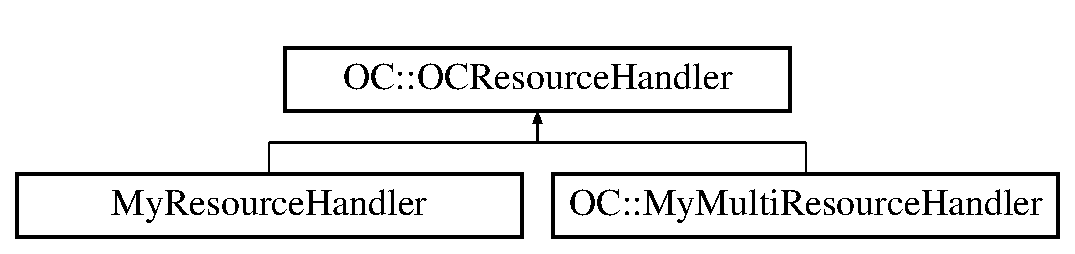
\includegraphics[height=2.000000cm]{classOC_1_1OCResourceHandler}
\end{center}
\end{figure}
\subsection*{Public Member Functions}
\begin{DoxyCompactItemize}
\item 
\hypertarget{classOC_1_1OCResourceHandler_af8e5c805c860206dafab508b732ea802}{}virtual void {\bfseries on\+Found\+Resource} (O\+C\+Resource\+Result $\ast$update, void $\ast$params)=0\label{classOC_1_1OCResourceHandler_af8e5c805c860206dafab508b732ea802}

\item 
\hypertarget{classOC_1_1OCResourceHandler_abf8d4bec38a1f81756f11c3058109498}{}virtual void {\bfseries on\+Completed} ()=0\label{classOC_1_1OCResourceHandler_abf8d4bec38a1f81756f11c3058109498}

\item 
\hypertarget{classOC_1_1OCResourceHandler_a0893d74e2b4ca3024f2e9ad832534642}{}virtual void {\bfseries on\+Failed} ()=0\label{classOC_1_1OCResourceHandler_a0893d74e2b4ca3024f2e9ad832534642}

\end{DoxyCompactItemize}


\subsection{Detailed Description}
\hyperlink{classOC_1_1OCResourceHandler}{O\+C\+Resource\+Handler} is a pure abstract class and it can be used for resource related callbacks. 

The documentation for this class was generated from the following file\+:\begin{DoxyCompactItemize}
\item 
/home/user/\+O\+I\+C/oic-\/resource/include/\hyperlink{OCResourceHandler_8h}{O\+C\+Resource\+Handler.\+h}\end{DoxyCompactItemize}

\hypertarget{classOC_1_1OCResourceRequest}{}\section{O\+C\+:\+:O\+C\+Resource\+Request Class Reference}
\label{classOC_1_1OCResourceRequest}\index{O\+C\+::\+O\+C\+Resource\+Request@{O\+C\+::\+O\+C\+Resource\+Request}}


\hyperlink{classOC_1_1OCResourceRequest}{O\+C\+Resource\+Request} provides A\+P\+Is to extract details from a request U\+R\+I.  




{\ttfamily \#include $<$O\+C\+Resource\+Request.\+h$>$}

\subsection*{Public Types}
\begin{DoxyCompactItemize}
\item 
\hypertarget{classOC_1_1OCResourceRequest_a9915455a27d7caba6b3f2bddae6b8ea8}{}typedef std\+::shared\+\_\+ptr$<$ \hyperlink{classOC_1_1OCResourceRequest}{O\+C\+Resource\+Request} $>$ {\bfseries Ptr}\label{classOC_1_1OCResourceRequest_a9915455a27d7caba6b3f2bddae6b8ea8}

\end{DoxyCompactItemize}
\subsection*{Public Member Functions}
\begin{DoxyCompactItemize}
\item 
virtual \hyperlink{classOC_1_1OCResourceRequest_af2fa22dc6bf6888c1cee9cbf9dc14cce}{$\sim$\+O\+C\+Resource\+Request} (void)
\item 
std\+::string \hyperlink{classOC_1_1OCResourceRequest_ab27a4deeb51e8039f1ca8b478cbd8440}{get\+Request\+Type} () const 
\item 
const Query\+Params\+Map \& \hyperlink{classOC_1_1OCResourceRequest_acc294d625957fbeae3ca1cd8a116c34b}{get\+Query\+Parameters} () const 
\item 
Request\+Handler\+Flag \hyperlink{classOC_1_1OCResourceRequest_a3db5684a64a20c7d7bbf648d7bcbd511}{get\+Request\+Handler\+Flag} () const 
\item 
const Attribute\+Map \& \hyperlink{classOC_1_1OCResourceRequest_ad08cd672748a7cd4fa1a7ceb8ef6abca}{get\+Attribute\+Representation} () const 
\item 
\hypertarget{classOC_1_1OCResourceRequest_a0f270c5c32afa64284f6e68bea61b350}{}const \hyperlink{classOC_1_1OCRepresentation}{O\+C\+Representation} \& {\bfseries get\+Resource\+Representation} () const \label{classOC_1_1OCResourceRequest_a0f270c5c32afa64284f6e68bea61b350}

\item 
\hypertarget{classOC_1_1OCResourceRequest_a07b269420d60dca8c0835a29c67d378e}{}void {\bfseries set\+Request\+Type} (const std\+::string \&request\+Type)\label{classOC_1_1OCResourceRequest_a07b269420d60dca8c0835a29c67d378e}

\item 
\hypertarget{classOC_1_1OCResourceRequest_a9f006f0707201b5c4def61c3a83b130a}{}void {\bfseries set\+Payload} (const std\+::string \&request\+Payload)\label{classOC_1_1OCResourceRequest_a9f006f0707201b5c4def61c3a83b130a}

\item 
\hypertarget{classOC_1_1OCResourceRequest_ae1d1738dacce9026d1b0502986e1739c}{}void {\bfseries set\+Query\+Params} (Query\+Params\+Map \&query\+Params)\label{classOC_1_1OCResourceRequest_ae1d1738dacce9026d1b0502986e1739c}

\item 
\hypertarget{classOC_1_1OCResourceRequest_a638843dd0adff94bea892f219a5285a1}{}void {\bfseries set\+Request\+Handler\+Flag} (Request\+Handler\+Flag request\+Handler\+Flag)\label{classOC_1_1OCResourceRequest_a638843dd0adff94bea892f219a5285a1}

\end{DoxyCompactItemize}


\subsection{Detailed Description}
\hyperlink{classOC_1_1OCResourceRequest}{O\+C\+Resource\+Request} provides A\+P\+Is to extract details from a request U\+R\+I. 

\subsection{Constructor \& Destructor Documentation}
\hypertarget{classOC_1_1OCResourceRequest_af2fa22dc6bf6888c1cee9cbf9dc14cce}{}\index{O\+C\+::\+O\+C\+Resource\+Request@{O\+C\+::\+O\+C\+Resource\+Request}!````~O\+C\+Resource\+Request@{$\sim$\+O\+C\+Resource\+Request}}
\index{````~O\+C\+Resource\+Request@{$\sim$\+O\+C\+Resource\+Request}!O\+C\+::\+O\+C\+Resource\+Request@{O\+C\+::\+O\+C\+Resource\+Request}}
\subsubsection[{$\sim$\+O\+C\+Resource\+Request}]{\setlength{\rightskip}{0pt plus 5cm}virtual O\+C\+::\+O\+C\+Resource\+Request\+::$\sim$\+O\+C\+Resource\+Request (
\begin{DoxyParamCaption}
\item[{void}]{}
\end{DoxyParamCaption}
)\hspace{0.3cm}{\ttfamily [inline]}, {\ttfamily [virtual]}}\label{classOC_1_1OCResourceRequest_af2fa22dc6bf6888c1cee9cbf9dc14cce}
Virtual destructor 

\subsection{Member Function Documentation}
\hypertarget{classOC_1_1OCResourceRequest_ad08cd672748a7cd4fa1a7ceb8ef6abca}{}\index{O\+C\+::\+O\+C\+Resource\+Request@{O\+C\+::\+O\+C\+Resource\+Request}!get\+Attribute\+Representation@{get\+Attribute\+Representation}}
\index{get\+Attribute\+Representation@{get\+Attribute\+Representation}!O\+C\+::\+O\+C\+Resource\+Request@{O\+C\+::\+O\+C\+Resource\+Request}}
\subsubsection[{get\+Attribute\+Representation}]{\setlength{\rightskip}{0pt plus 5cm}const Attribute\+Map\& O\+C\+::\+O\+C\+Resource\+Request\+::get\+Attribute\+Representation (
\begin{DoxyParamCaption}
{}
\end{DoxyParamCaption}
) const\hspace{0.3cm}{\ttfamily [inline]}}\label{classOC_1_1OCResourceRequest_ad08cd672748a7cd4fa1a7ceb8ef6abca}
Provides the entire resource attribute representation \begin{DoxyReturn}{Returns}
std\+::map Attribute\+Map reference containing the name value pairs representing the resource's attributes 
\end{DoxyReturn}
\hypertarget{classOC_1_1OCResourceRequest_acc294d625957fbeae3ca1cd8a116c34b}{}\index{O\+C\+::\+O\+C\+Resource\+Request@{O\+C\+::\+O\+C\+Resource\+Request}!get\+Query\+Parameters@{get\+Query\+Parameters}}
\index{get\+Query\+Parameters@{get\+Query\+Parameters}!O\+C\+::\+O\+C\+Resource\+Request@{O\+C\+::\+O\+C\+Resource\+Request}}
\subsubsection[{get\+Query\+Parameters}]{\setlength{\rightskip}{0pt plus 5cm}const Query\+Params\+Map\& O\+C\+::\+O\+C\+Resource\+Request\+::get\+Query\+Parameters (
\begin{DoxyParamCaption}
{}
\end{DoxyParamCaption}
) const\hspace{0.3cm}{\ttfamily [inline]}}\label{classOC_1_1OCResourceRequest_acc294d625957fbeae3ca1cd8a116c34b}
Retrieves the query parameters from the request \begin{DoxyReturn}{Returns}
std\+::string query parameters in the request 
\end{DoxyReturn}
\hypertarget{classOC_1_1OCResourceRequest_a3db5684a64a20c7d7bbf648d7bcbd511}{}\index{O\+C\+::\+O\+C\+Resource\+Request@{O\+C\+::\+O\+C\+Resource\+Request}!get\+Request\+Handler\+Flag@{get\+Request\+Handler\+Flag}}
\index{get\+Request\+Handler\+Flag@{get\+Request\+Handler\+Flag}!O\+C\+::\+O\+C\+Resource\+Request@{O\+C\+::\+O\+C\+Resource\+Request}}
\subsubsection[{get\+Request\+Handler\+Flag}]{\setlength{\rightskip}{0pt plus 5cm}Request\+Handler\+Flag O\+C\+::\+O\+C\+Resource\+Request\+::get\+Request\+Handler\+Flag (
\begin{DoxyParamCaption}
{}
\end{DoxyParamCaption}
) const\hspace{0.3cm}{\ttfamily [inline]}}\label{classOC_1_1OCResourceRequest_a3db5684a64a20c7d7bbf648d7bcbd511}
Retrieves the request handler flag type. This can be either I\+N\+I\+T flag or R\+E\+Q\+U\+E\+S\+T flag or O\+B\+S\+E\+R\+V\+E flag. N\+O\+T\+E\+: I\+N\+I\+T indicates that the vendor's entity handler should go and perform initialization operations R\+E\+Q\+U\+E\+S\+T indicates that it is a request of certain type (G\+E\+T/\+P\+U\+T/\+P\+O\+S\+T/\+D\+E\+L\+E\+T\+E) and entity handler needs to perform corresponding operations O\+B\+S\+E\+R\+V\+E indicates that the request is of type Observe and entity handler needs to perform corresponding operations \begin{DoxyReturn}{Returns}
std\+::string type of request flag 
\end{DoxyReturn}
\hypertarget{classOC_1_1OCResourceRequest_ab27a4deeb51e8039f1ca8b478cbd8440}{}\index{O\+C\+::\+O\+C\+Resource\+Request@{O\+C\+::\+O\+C\+Resource\+Request}!get\+Request\+Type@{get\+Request\+Type}}
\index{get\+Request\+Type@{get\+Request\+Type}!O\+C\+::\+O\+C\+Resource\+Request@{O\+C\+::\+O\+C\+Resource\+Request}}
\subsubsection[{get\+Request\+Type}]{\setlength{\rightskip}{0pt plus 5cm}std\+::string O\+C\+::\+O\+C\+Resource\+Request\+::get\+Request\+Type (
\begin{DoxyParamCaption}
{}
\end{DoxyParamCaption}
) const\hspace{0.3cm}{\ttfamily [inline]}}\label{classOC_1_1OCResourceRequest_ab27a4deeb51e8039f1ca8b478cbd8440}
Retrieves the type of request string for the entity handler function to operate \begin{DoxyReturn}{Returns}
std\+::string request type. This could be 'G\+E\+T'/'P\+U\+T'/'P\+O\+S\+T'/'D\+E\+L\+E\+T\+E' 
\end{DoxyReturn}


The documentation for this class was generated from the following file\+:\begin{DoxyCompactItemize}
\item 
/home/user/\+O\+I\+C/oic-\/resource/include/\hyperlink{OCResourceRequest_8h}{O\+C\+Resource\+Request.\+h}\end{DoxyCompactItemize}

\hypertarget{classOC_1_1OCResourceResponse}{}\section{O\+C\+:\+:O\+C\+Resource\+Response Class Reference}
\label{classOC_1_1OCResourceResponse}\index{O\+C\+::\+O\+C\+Resource\+Response@{O\+C\+::\+O\+C\+Resource\+Response}}


\hyperlink{classOC_1_1OCResourceResponse}{O\+C\+Resource\+Response} provides A\+P\+Is to set the response details.  




{\ttfamily \#include $<$O\+C\+Resource\+Response.\+h$>$}

\subsection*{Public Types}
\begin{DoxyCompactItemize}
\item 
\hypertarget{classOC_1_1OCResourceResponse_aa1041e7d85a532f1ae0896d3a1d8d5aa}{}typedef std\+::shared\+\_\+ptr$<$ \hyperlink{classOC_1_1OCResourceResponse}{O\+C\+Resource\+Response} $>$ {\bfseries Ptr}\label{classOC_1_1OCResourceResponse_aa1041e7d85a532f1ae0896d3a1d8d5aa}

\end{DoxyCompactItemize}
\subsection*{Public Member Functions}
\begin{DoxyCompactItemize}
\item 
\hyperlink{classOC_1_1OCResourceResponse_ac4f7ddf88b36476c6a794be31e58fb8e}{O\+C\+Resource\+Response} ()
\item 
virtual \hyperlink{classOC_1_1OCResourceResponse_ae9531db0616407410535be8ef56e0f8f}{$\sim$\+O\+C\+Resource\+Response} (void)
\item 
void \hyperlink{classOC_1_1OCResourceResponse_af4f60806fc32df38799532ea4cf6d9c4}{set\+Error\+Code} (const int e\+Code)
\item 
void \hyperlink{classOC_1_1OCResourceResponse_aa26e157cb217d3486b6b6848ba241263}{set\+Resource\+Representation} (\hyperlink{classOC_1_1OCRepresentation}{O\+C\+Representation} \&rep, std\+::string interface)
\item 
void \hyperlink{classOC_1_1OCResourceResponse_adcefb4320aca3287d144c31c5539584a}{set\+Resource\+Representation\+L\+L} (\hyperlink{classOC_1_1OCRepresentation}{O\+C\+Representation} \&rep)
\item 
void \hyperlink{classOC_1_1OCResourceResponse_a36e5f5fe7f6a595db436a23536fc7cbc}{set\+Resource\+Representation\+Default} (\hyperlink{classOC_1_1OCRepresentation}{O\+C\+Representation} \&rep)
\item 
void \hyperlink{classOC_1_1OCResourceResponse_afd38a03154baa6b78cd26d33ec304cdb}{set\+Resource\+Representation\+Batch} (\hyperlink{classOC_1_1OCRepresentation}{O\+C\+Representation} \&rep)
\item 
void \hyperlink{classOC_1_1OCResourceResponse_aa2638af45ad173ffbf9a41e0c9ace13b}{set\+Resource\+Representation} (Attribute\+Map \&attributes)
\item 
int \hyperlink{classOC_1_1OCResourceResponse_ae88df3aa94f441634f5f8b775bcf9ec8}{get\+Error\+Code} () const 
\item 
Attribute\+Map \& \hyperlink{classOC_1_1OCResourceResponse_a94f1db85fa52b3f7a2b913fa544b732e}{get\+Resource\+Representation} () const 
\item 
\hypertarget{classOC_1_1OCResourceResponse_aac29e48fe8cfa463a63a6197065b4899}{}std\+::string {\bfseries get\+Payload} ()\label{classOC_1_1OCResourceResponse_aac29e48fe8cfa463a63a6197065b4899}

\end{DoxyCompactItemize}


\subsection{Detailed Description}
\hyperlink{classOC_1_1OCResourceResponse}{O\+C\+Resource\+Response} provides A\+P\+Is to set the response details. 

\subsection{Constructor \& Destructor Documentation}
\hypertarget{classOC_1_1OCResourceResponse_ac4f7ddf88b36476c6a794be31e58fb8e}{}\index{O\+C\+::\+O\+C\+Resource\+Response@{O\+C\+::\+O\+C\+Resource\+Response}!O\+C\+Resource\+Response@{O\+C\+Resource\+Response}}
\index{O\+C\+Resource\+Response@{O\+C\+Resource\+Response}!O\+C\+::\+O\+C\+Resource\+Response@{O\+C\+::\+O\+C\+Resource\+Response}}
\subsubsection[{O\+C\+Resource\+Response}]{\setlength{\rightskip}{0pt plus 5cm}O\+C\+::\+O\+C\+Resource\+Response\+::\+O\+C\+Resource\+Response (
\begin{DoxyParamCaption}
{}
\end{DoxyParamCaption}
)\hspace{0.3cm}{\ttfamily [inline]}}\label{classOC_1_1OCResourceResponse_ac4f7ddf88b36476c6a794be31e58fb8e}
Default destructor \hypertarget{classOC_1_1OCResourceResponse_ae9531db0616407410535be8ef56e0f8f}{}\index{O\+C\+::\+O\+C\+Resource\+Response@{O\+C\+::\+O\+C\+Resource\+Response}!````~O\+C\+Resource\+Response@{$\sim$\+O\+C\+Resource\+Response}}
\index{````~O\+C\+Resource\+Response@{$\sim$\+O\+C\+Resource\+Response}!O\+C\+::\+O\+C\+Resource\+Response@{O\+C\+::\+O\+C\+Resource\+Response}}
\subsubsection[{$\sim$\+O\+C\+Resource\+Response}]{\setlength{\rightskip}{0pt plus 5cm}virtual O\+C\+::\+O\+C\+Resource\+Response\+::$\sim$\+O\+C\+Resource\+Response (
\begin{DoxyParamCaption}
\item[{void}]{}
\end{DoxyParamCaption}
)\hspace{0.3cm}{\ttfamily [inline]}, {\ttfamily [virtual]}}\label{classOC_1_1OCResourceResponse_ae9531db0616407410535be8ef56e0f8f}
Virtual destructor 

\subsection{Member Function Documentation}
\hypertarget{classOC_1_1OCResourceResponse_ae88df3aa94f441634f5f8b775bcf9ec8}{}\index{O\+C\+::\+O\+C\+Resource\+Response@{O\+C\+::\+O\+C\+Resource\+Response}!get\+Error\+Code@{get\+Error\+Code}}
\index{get\+Error\+Code@{get\+Error\+Code}!O\+C\+::\+O\+C\+Resource\+Response@{O\+C\+::\+O\+C\+Resource\+Response}}
\subsubsection[{get\+Error\+Code}]{\setlength{\rightskip}{0pt plus 5cm}int O\+C\+::\+O\+C\+Resource\+Response\+::get\+Error\+Code (
\begin{DoxyParamCaption}
{}
\end{DoxyParamCaption}
) const}\label{classOC_1_1OCResourceResponse_ae88df3aa94f441634f5f8b775bcf9ec8}
Get error code \hypertarget{classOC_1_1OCResourceResponse_a94f1db85fa52b3f7a2b913fa544b732e}{}\index{O\+C\+::\+O\+C\+Resource\+Response@{O\+C\+::\+O\+C\+Resource\+Response}!get\+Resource\+Representation@{get\+Resource\+Representation}}
\index{get\+Resource\+Representation@{get\+Resource\+Representation}!O\+C\+::\+O\+C\+Resource\+Response@{O\+C\+::\+O\+C\+Resource\+Response}}
\subsubsection[{get\+Resource\+Representation}]{\setlength{\rightskip}{0pt plus 5cm}Attribute\+Map\& O\+C\+::\+O\+C\+Resource\+Response\+::get\+Resource\+Representation (
\begin{DoxyParamCaption}
{}
\end{DoxyParamCaption}
) const}\label{classOC_1_1OCResourceResponse_a94f1db85fa52b3f7a2b913fa544b732e}
Get the resource attribute representation \hypertarget{classOC_1_1OCResourceResponse_af4f60806fc32df38799532ea4cf6d9c4}{}\index{O\+C\+::\+O\+C\+Resource\+Response@{O\+C\+::\+O\+C\+Resource\+Response}!set\+Error\+Code@{set\+Error\+Code}}
\index{set\+Error\+Code@{set\+Error\+Code}!O\+C\+::\+O\+C\+Resource\+Response@{O\+C\+::\+O\+C\+Resource\+Response}}
\subsubsection[{set\+Error\+Code}]{\setlength{\rightskip}{0pt plus 5cm}void O\+C\+::\+O\+C\+Resource\+Response\+::set\+Error\+Code (
\begin{DoxyParamCaption}
\item[{const int}]{e\+Code}
\end{DoxyParamCaption}
)\hspace{0.3cm}{\ttfamily [inline]}}\label{classOC_1_1OCResourceResponse_af4f60806fc32df38799532ea4cf6d9c4}
This A\+P\+I sets the error code for this response 
\begin{DoxyParams}{Parameters}
{\em e\+Code} & error code to set \\
\hline
\end{DoxyParams}
\hypertarget{classOC_1_1OCResourceResponse_aa26e157cb217d3486b6b6848ba241263}{}\index{O\+C\+::\+O\+C\+Resource\+Response@{O\+C\+::\+O\+C\+Resource\+Response}!set\+Resource\+Representation@{set\+Resource\+Representation}}
\index{set\+Resource\+Representation@{set\+Resource\+Representation}!O\+C\+::\+O\+C\+Resource\+Response@{O\+C\+::\+O\+C\+Resource\+Response}}
\subsubsection[{set\+Resource\+Representation}]{\setlength{\rightskip}{0pt plus 5cm}void O\+C\+::\+O\+C\+Resource\+Response\+::set\+Resource\+Representation (
\begin{DoxyParamCaption}
\item[{{\bf O\+C\+Representation} \&}]{rep, }
\item[{std\+::string}]{interface}
\end{DoxyParamCaption}
)\hspace{0.3cm}{\ttfamily [inline]}}\label{classOC_1_1OCResourceResponse_aa26e157cb217d3486b6b6848ba241263}
A\+P\+I to set the entire resource attribute representation (B\+A\+T\+C\+H) 
\begin{DoxyParams}{Parameters}
{\em attribute\+Map} & reference containing the name value pairs representing the resource's attributes \\
\hline
\end{DoxyParams}
\hypertarget{classOC_1_1OCResourceResponse_aa2638af45ad173ffbf9a41e0c9ace13b}{}\index{O\+C\+::\+O\+C\+Resource\+Response@{O\+C\+::\+O\+C\+Resource\+Response}!set\+Resource\+Representation@{set\+Resource\+Representation}}
\index{set\+Resource\+Representation@{set\+Resource\+Representation}!O\+C\+::\+O\+C\+Resource\+Response@{O\+C\+::\+O\+C\+Resource\+Response}}
\subsubsection[{set\+Resource\+Representation}]{\setlength{\rightskip}{0pt plus 5cm}void O\+C\+::\+O\+C\+Resource\+Response\+::set\+Resource\+Representation (
\begin{DoxyParamCaption}
\item[{Attribute\+Map \&}]{attributes}
\end{DoxyParamCaption}
)\hspace{0.3cm}{\ttfamily [inline]}}\label{classOC_1_1OCResourceResponse_aa2638af45ad173ffbf9a41e0c9ace13b}
T\+O\+D\+O remove this once after above function stabilize. A\+P\+I to set the entire resource attribute representation 
\begin{DoxyParams}{Parameters}
{\em attribute\+Map} & reference containing the name value pairs representing the resource's attributes \\
\hline
\end{DoxyParams}
\hypertarget{classOC_1_1OCResourceResponse_afd38a03154baa6b78cd26d33ec304cdb}{}\index{O\+C\+::\+O\+C\+Resource\+Response@{O\+C\+::\+O\+C\+Resource\+Response}!set\+Resource\+Representation\+Batch@{set\+Resource\+Representation\+Batch}}
\index{set\+Resource\+Representation\+Batch@{set\+Resource\+Representation\+Batch}!O\+C\+::\+O\+C\+Resource\+Response@{O\+C\+::\+O\+C\+Resource\+Response}}
\subsubsection[{set\+Resource\+Representation\+Batch}]{\setlength{\rightskip}{0pt plus 5cm}void O\+C\+::\+O\+C\+Resource\+Response\+::set\+Resource\+Representation\+Batch (
\begin{DoxyParamCaption}
\item[{{\bf O\+C\+Representation} \&}]{rep}
\end{DoxyParamCaption}
)\hspace{0.3cm}{\ttfamily [inline]}}\label{classOC_1_1OCResourceResponse_afd38a03154baa6b78cd26d33ec304cdb}
A\+P\+I to set the entire resource attribute representation (B\+A\+T\+C\+H) 
\begin{DoxyParams}{Parameters}
{\em attribute\+Map} & reference containing the name value pairs representing the resource's attributes \\
\hline
\end{DoxyParams}
\hypertarget{classOC_1_1OCResourceResponse_a36e5f5fe7f6a595db436a23536fc7cbc}{}\index{O\+C\+::\+O\+C\+Resource\+Response@{O\+C\+::\+O\+C\+Resource\+Response}!set\+Resource\+Representation\+Default@{set\+Resource\+Representation\+Default}}
\index{set\+Resource\+Representation\+Default@{set\+Resource\+Representation\+Default}!O\+C\+::\+O\+C\+Resource\+Response@{O\+C\+::\+O\+C\+Resource\+Response}}
\subsubsection[{set\+Resource\+Representation\+Default}]{\setlength{\rightskip}{0pt plus 5cm}void O\+C\+::\+O\+C\+Resource\+Response\+::set\+Resource\+Representation\+Default (
\begin{DoxyParamCaption}
\item[{{\bf O\+C\+Representation} \&}]{rep}
\end{DoxyParamCaption}
)\hspace{0.3cm}{\ttfamily [inline]}}\label{classOC_1_1OCResourceResponse_a36e5f5fe7f6a595db436a23536fc7cbc}
A\+P\+I to set the entire resource attribute representation (Default)) 
\begin{DoxyParams}{Parameters}
{\em attribute\+Map} & reference containing the name value pairs representing the resource's attributes \\
\hline
\end{DoxyParams}
\hypertarget{classOC_1_1OCResourceResponse_adcefb4320aca3287d144c31c5539584a}{}\index{O\+C\+::\+O\+C\+Resource\+Response@{O\+C\+::\+O\+C\+Resource\+Response}!set\+Resource\+Representation\+L\+L@{set\+Resource\+Representation\+L\+L}}
\index{set\+Resource\+Representation\+L\+L@{set\+Resource\+Representation\+L\+L}!O\+C\+::\+O\+C\+Resource\+Response@{O\+C\+::\+O\+C\+Resource\+Response}}
\subsubsection[{set\+Resource\+Representation\+L\+L}]{\setlength{\rightskip}{0pt plus 5cm}void O\+C\+::\+O\+C\+Resource\+Response\+::set\+Resource\+Representation\+L\+L (
\begin{DoxyParamCaption}
\item[{{\bf O\+C\+Representation} \&}]{rep}
\end{DoxyParamCaption}
)\hspace{0.3cm}{\ttfamily [inline]}}\label{classOC_1_1OCResourceResponse_adcefb4320aca3287d144c31c5539584a}
A\+P\+I to set the entire resource attribute representation (Linked List Interface)) 
\begin{DoxyParams}{Parameters}
{\em attribute\+Map} & reference containing the name value pairs representing the resource's attributes \\
\hline
\end{DoxyParams}


The documentation for this class was generated from the following file\+:\begin{DoxyCompactItemize}
\item 
/home/user/\+O\+I\+C/oic-\/resource/include/\hyperlink{OCResourceResponse_8h}{O\+C\+Resource\+Response.\+h}\end{DoxyCompactItemize}

\hypertarget{structOCResponse}{}\section{O\+C\+Response Struct Reference}
\label{structOCResponse}\index{O\+C\+Response@{O\+C\+Response}}
\subsection*{Public Attributes}
\begin{DoxyCompactItemize}
\item 
\hypertarget{structOCResponse_a468e3d857bf47816f70b87e487c91e7e}{}\hyperlink{structClientCB}{Client\+C\+B} $\ast$ {\bfseries cb\+Node}\label{structOCResponse_a468e3d857bf47816f70b87e487c91e7e}

\item 
\hypertarget{structOCResponse_a25d4ff7a51f5bf424f017d1d44f5774c}{}uint32\+\_\+t {\bfseries T\+T\+L}\label{structOCResponse_a25d4ff7a51f5bf424f017d1d44f5774c}

\item 
\hypertarget{structOCResponse_ad2e5d6958e3d56c17d147fcd0b56b010}{}\hyperlink{structOCClientResponse}{O\+C\+Client\+Response} $\ast$ {\bfseries client\+Response}\label{structOCResponse_ad2e5d6958e3d56c17d147fcd0b56b010}

\end{DoxyCompactItemize}


The documentation for this struct was generated from the following file\+:\begin{DoxyCompactItemize}
\item 
/home/user/\+O\+I\+C/oic-\/resource/csdk/stack/include/internal/ocstackinternal.\+h\end{DoxyCompactItemize}

\hypertarget{classOC_1_1OCSecurityModel}{}\section{O\+C\+:\+:O\+C\+Security\+Model Class Reference}
\label{classOC_1_1OCSecurityModel}\index{O\+C\+::\+O\+C\+Security\+Model@{O\+C\+::\+O\+C\+Security\+Model}}


This class provides the required security model to access a service or a particular resource.  




{\ttfamily \#include $<$O\+C\+Security\+Model.\+h$>$}

\subsection*{Public Member Functions}
\begin{DoxyCompactItemize}
\item 
\hypertarget{classOC_1_1OCSecurityModel_af4a889dc952e0269fe55b6ead58875eb}{}void {\bfseries check\+Access} (U\+R\+I source\+U\+R\+I, U\+R\+I destination\+U\+R\+I, int encryption\+Level, int remote\+Identity)\label{classOC_1_1OCSecurityModel_af4a889dc952e0269fe55b6ead58875eb}

\end{DoxyCompactItemize}


\subsection{Detailed Description}
This class provides the required security model to access a service or a particular resource. 

The documentation for this class was generated from the following file\+:\begin{DoxyCompactItemize}
\item 
/home/user/\+O\+I\+C/oic-\/resource/include/\hyperlink{OCSecurityModel_8h}{O\+C\+Security\+Model.\+h}\end{DoxyCompactItemize}

\hypertarget{classOC_1_1OutOfProcClientWrapper}{}\section{O\+C\+:\+:Out\+Of\+Proc\+Client\+Wrapper Class Reference}
\label{classOC_1_1OutOfProcClientWrapper}\index{O\+C\+::\+Out\+Of\+Proc\+Client\+Wrapper@{O\+C\+::\+Out\+Of\+Proc\+Client\+Wrapper}}
Inheritance diagram for O\+C\+:\+:Out\+Of\+Proc\+Client\+Wrapper\+:\begin{figure}[H]
\begin{center}
\leavevmode
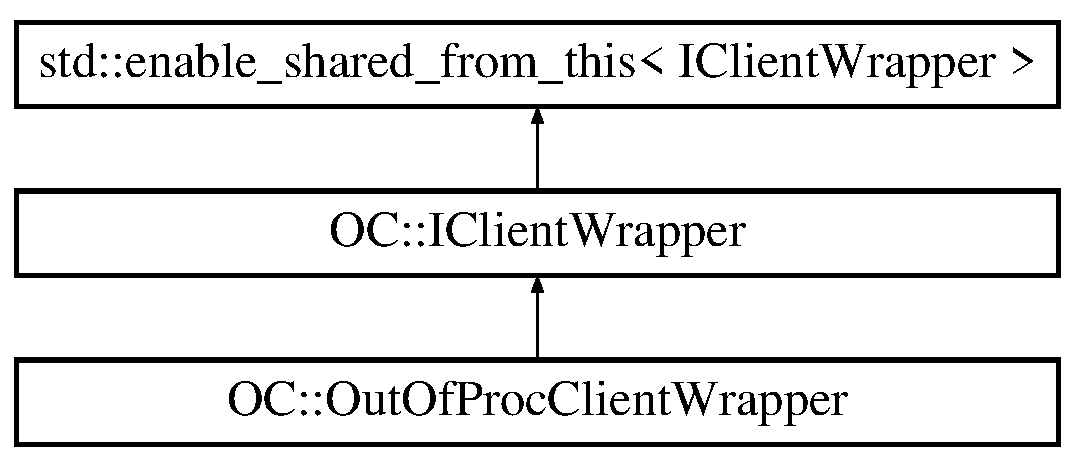
\includegraphics[height=3.000000cm]{classOC_1_1OutOfProcClientWrapper}
\end{center}
\end{figure}
\subsection*{Public Member Functions}
\begin{DoxyCompactItemize}
\item 
\hypertarget{classOC_1_1OutOfProcClientWrapper_a4d6728f802b9a06d1a35eb240fc1ca97}{}{\bfseries Out\+Of\+Proc\+Client\+Wrapper} (std\+::weak\+\_\+ptr$<$ std\+::mutex $>$ csdk\+Lock, \hyperlink{structOC_1_1PlatformConfig}{Platform\+Config} cfg)\label{classOC_1_1OutOfProcClientWrapper_a4d6728f802b9a06d1a35eb240fc1ca97}

\item 
\hypertarget{classOC_1_1OutOfProcClientWrapper_aa0e27789618d48ca5c40554b91b79666}{}virtual O\+C\+Stack\+Result {\bfseries Listen\+For\+Resource} (const std\+::string \&service\+Url, const std\+::string \&resource\+Type, Find\+Callback \&callback)\label{classOC_1_1OutOfProcClientWrapper_aa0e27789618d48ca5c40554b91b79666}

\item 
\hypertarget{classOC_1_1OutOfProcClientWrapper_a79d0602b43dfa5e832cce1562b301b1e}{}virtual O\+C\+Stack\+Result {\bfseries Get\+Resource\+Attributes} (const std\+::string \&host, const std\+::string \&uri, const Query\+Params\+Map \&query\+Params, Get\+Callback \&callback)\label{classOC_1_1OutOfProcClientWrapper_a79d0602b43dfa5e832cce1562b301b1e}

\item 
\hypertarget{classOC_1_1OutOfProcClientWrapper_a2d46393d23661e184353f8f8689b2c43}{}virtual O\+C\+Stack\+Result {\bfseries Set\+Resource\+Attributes} (const std\+::string \&host, const std\+::string \&uri, const \hyperlink{classOC_1_1OCRepresentation}{O\+C\+Representation} \&attributes, const Query\+Params\+Map \&query\+Params, Put\+Callback \&callback)\label{classOC_1_1OutOfProcClientWrapper_a2d46393d23661e184353f8f8689b2c43}

\item 
\hypertarget{classOC_1_1OutOfProcClientWrapper_aafcad1f35ca292ecf713bfa57119792d}{}virtual O\+C\+Stack\+Result {\bfseries Observe\+Resource} (Observe\+Type observe\+Type, O\+C\+Do\+Handle $\ast$handle, const std\+::string \&host, const std\+::string \&uri, const Query\+Params\+Map \&query\+Params, Observe\+Callback \&callback)\label{classOC_1_1OutOfProcClientWrapper_aafcad1f35ca292ecf713bfa57119792d}

\item 
\hypertarget{classOC_1_1OutOfProcClientWrapper_a843a43b35a597eef9388758c38349098}{}virtual O\+C\+Stack\+Result {\bfseries Cancel\+Observe\+Resource} (O\+C\+Do\+Handle handle, const std\+::string \&host, const std\+::string \&uri)\label{classOC_1_1OutOfProcClientWrapper_a843a43b35a597eef9388758c38349098}

\item 
\hypertarget{classOC_1_1OutOfProcClientWrapper_a2038efbb54810e76b816731bb566e0b3}{}virtual std\+::shared\+\_\+ptr$<$ \hyperlink{classOC_1_1OCResource}{O\+C\+Resource} $>$ {\bfseries parse\+O\+C\+Resource} (I\+Client\+Wrapper\+::\+Ptr client\+Wrapper, const std\+::string \&host, const boost\+::property\+\_\+tree\+::ptree resource\+Node)\label{classOC_1_1OutOfProcClientWrapper_a2038efbb54810e76b816731bb566e0b3}

\item 
\hypertarget{classOC_1_1OutOfProcClientWrapper_ad7142a92eb637a344364cb123a1511eb}{}virtual O\+C\+Stack\+Result {\bfseries Subscribe\+Presence} (O\+C\+Do\+Handle $\ast$handle, const std\+::string \&host, Subscribe\+Callback \&presence\+Handler)\label{classOC_1_1OutOfProcClientWrapper_ad7142a92eb637a344364cb123a1511eb}

\item 
\hypertarget{classOC_1_1OutOfProcClientWrapper_a933522d46114355eba91f7d7ee1a5db2}{}virtual O\+C\+Stack\+Result {\bfseries Unsubscribe\+Presence} (O\+C\+Do\+Handle handle)\label{classOC_1_1OutOfProcClientWrapper_a933522d46114355eba91f7d7ee1a5db2}

\end{DoxyCompactItemize}
\subsection*{Additional Inherited Members}


The documentation for this class was generated from the following file\+:\begin{DoxyCompactItemize}
\item 
/home/user/\+O\+I\+C/oic-\/resource/include/Out\+Of\+Proc\+Client\+Wrapper.\+h\end{DoxyCompactItemize}

\hypertarget{classOC_1_1OutOfProcServerWrapper}{}\section{O\+C\+:\+:Out\+Of\+Proc\+Server\+Wrapper Class Reference}
\label{classOC_1_1OutOfProcServerWrapper}\index{O\+C\+::\+Out\+Of\+Proc\+Server\+Wrapper@{O\+C\+::\+Out\+Of\+Proc\+Server\+Wrapper}}
Inheritance diagram for O\+C\+:\+:Out\+Of\+Proc\+Server\+Wrapper\+:\begin{figure}[H]
\begin{center}
\leavevmode
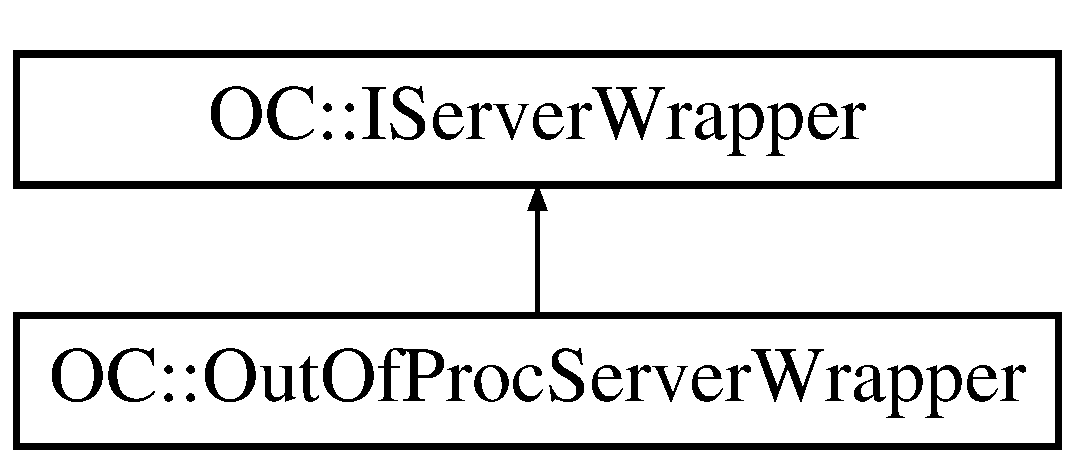
\includegraphics[height=2.000000cm]{classOC_1_1OutOfProcServerWrapper}
\end{center}
\end{figure}
\subsection*{Public Member Functions}
\begin{DoxyCompactItemize}
\item 
\hypertarget{classOC_1_1OutOfProcServerWrapper_aa0ca66b894b695679b8939fa7e4f2f69}{}{\bfseries Out\+Of\+Proc\+Server\+Wrapper} (\hyperlink{structOC_1_1PlatformConfig}{Platform\+Config} cfg)\label{classOC_1_1OutOfProcServerWrapper_aa0ca66b894b695679b8939fa7e4f2f69}

\item 
\hypertarget{classOC_1_1OutOfProcServerWrapper_a0c7ad538f0d7bad991899adead71f647}{}virtual O\+C\+Stack\+Result {\bfseries register\+Resource} (O\+C\+Resource\+Handle \&resource\+Handle, std\+::string \&resource\+U\+R\+I, const std\+::string \&resource\+Type\+Name, const std\+::string \&resource\+Interface, Register\+Callback \&entity\+Handler, uint8\+\_\+t resource\+Property)\label{classOC_1_1OutOfProcServerWrapper_a0c7ad538f0d7bad991899adead71f647}

\item 
\hypertarget{classOC_1_1OutOfProcServerWrapper_a861fee4fc14de26296f20cf89ccf7e6b}{}virtual O\+C\+Stack\+Result {\bfseries unregister\+Resource} (const O\+C\+Resource\+Handle \&resource\+Handle)\label{classOC_1_1OutOfProcServerWrapper_a861fee4fc14de26296f20cf89ccf7e6b}

\item 
\hypertarget{classOC_1_1OutOfProcServerWrapper_a4cf86674aab5df9f9073d93dd7cd0613}{}virtual O\+C\+Stack\+Result {\bfseries bind\+Type\+To\+Resource} (const O\+C\+Resource\+Handle \&resource\+Handle, const std\+::string \&resource\+Type\+Name)\label{classOC_1_1OutOfProcServerWrapper_a4cf86674aab5df9f9073d93dd7cd0613}

\item 
\hypertarget{classOC_1_1OutOfProcServerWrapper_aba73691be61c48b90ef829dc09a6ca67}{}virtual O\+C\+Stack\+Result {\bfseries bind\+Interface\+To\+Resource} (const O\+C\+Resource\+Handle \&resource\+Handle, const std\+::string \&resource\+Interface\+Name)\label{classOC_1_1OutOfProcServerWrapper_aba73691be61c48b90ef829dc09a6ca67}

\item 
\hypertarget{classOC_1_1OutOfProcServerWrapper_a2288984431b7d429c7795616496781ff}{}virtual O\+C\+Stack\+Result {\bfseries start\+Presence} (const unsigned int seconds)\label{classOC_1_1OutOfProcServerWrapper_a2288984431b7d429c7795616496781ff}

\item 
\hypertarget{classOC_1_1OutOfProcServerWrapper_afd686e2be1b82ec694cfbf8edda0599e}{}virtual O\+C\+Stack\+Result {\bfseries stop\+Presence} ()\label{classOC_1_1OutOfProcServerWrapper_afd686e2be1b82ec694cfbf8edda0599e}

\end{DoxyCompactItemize}
\subsection*{Additional Inherited Members}


The documentation for this class was generated from the following file\+:\begin{DoxyCompactItemize}
\item 
/home/user/\+O\+I\+C/oic-\/resource/include/Out\+Of\+Proc\+Server\+Wrapper.\+h\end{DoxyCompactItemize}

\hypertarget{structOC_1_1PlatformConfig}{}\section{O\+C\+:\+:Platform\+Config Struct Reference}
\label{structOC_1_1PlatformConfig}\index{O\+C\+::\+Platform\+Config@{O\+C\+::\+Platform\+Config}}
\subsection*{Public Member Functions}
\begin{DoxyCompactItemize}
\item 
\hypertarget{structOC_1_1PlatformConfig_add07f9a72830885112ff96ffc1d158f0}{}{\bfseries Platform\+Config} (const Service\+Type service\+Type\+\_\+, const Mode\+Type mode\+\_\+, const std\+::string \&ip\+Address\+\_\+, const uint16\+\_\+t port\+\_\+, const Quality\+Of\+Service Qo\+S\+\_\+)\label{structOC_1_1PlatformConfig_add07f9a72830885112ff96ffc1d158f0}

\end{DoxyCompactItemize}
\subsection*{Public Attributes}
\begin{DoxyCompactItemize}
\item 
\hypertarget{structOC_1_1PlatformConfig_a025d0ea30e2db9632346200f4268d8f8}{}Service\+Type {\bfseries service\+Type}\label{structOC_1_1PlatformConfig_a025d0ea30e2db9632346200f4268d8f8}

\item 
\hypertarget{structOC_1_1PlatformConfig_a3d89346c486be2884964a636a351039e}{}Mode\+Type {\bfseries mode}\label{structOC_1_1PlatformConfig_a3d89346c486be2884964a636a351039e}

\item 
\hypertarget{structOC_1_1PlatformConfig_a1b37e817bb3273fe6fd6831adbb42b94}{}std\+::string {\bfseries ip\+Address}\label{structOC_1_1PlatformConfig_a1b37e817bb3273fe6fd6831adbb42b94}

\item 
\hypertarget{structOC_1_1PlatformConfig_a74bdb44dc9b385b49b3d1e67d56174ed}{}uint16\+\_\+t {\bfseries port}\label{structOC_1_1PlatformConfig_a74bdb44dc9b385b49b3d1e67d56174ed}

\item 
\hypertarget{structOC_1_1PlatformConfig_a85554e5b5f967a7db287e467409f909b}{}Quality\+Of\+Service {\bfseries Qo\+S}\label{structOC_1_1PlatformConfig_a85554e5b5f967a7db287e467409f909b}

\end{DoxyCompactItemize}


The documentation for this struct was generated from the following file\+:\begin{DoxyCompactItemize}
\item 
/home/user/\+O\+I\+C/oic-\/resource/include/O\+C\+Api.\+h\end{DoxyCompactItemize}

\hypertarget{classOC_1_1ResourceInitException}{}\section{O\+C\+:\+:Resource\+Init\+Exception Class Reference}
\label{classOC_1_1ResourceInitException}\index{O\+C\+::\+Resource\+Init\+Exception@{O\+C\+::\+Resource\+Init\+Exception}}
Inheritance diagram for O\+C\+:\+:Resource\+Init\+Exception\+:\begin{figure}[H]
\begin{center}
\leavevmode
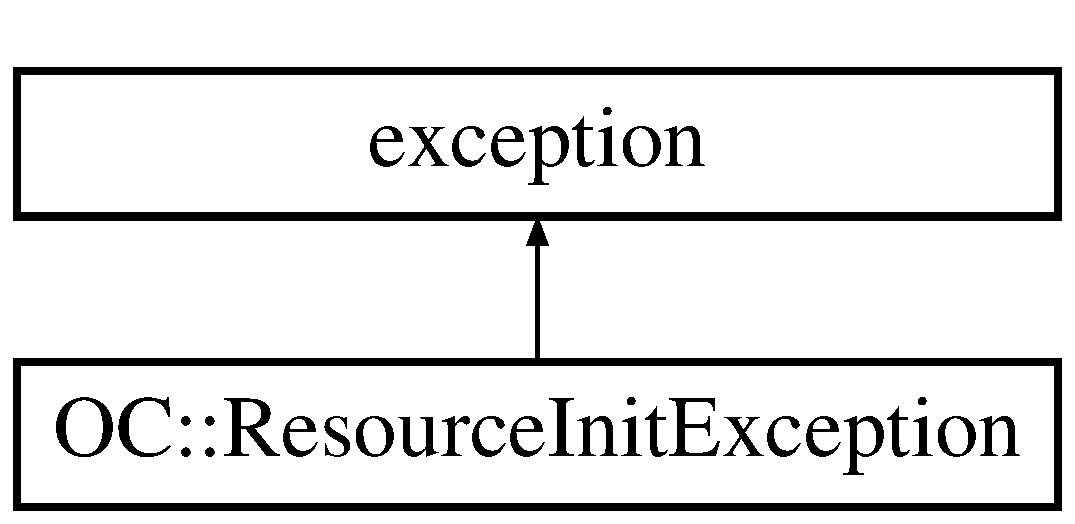
\includegraphics[height=2.000000cm]{classOC_1_1ResourceInitException}
\end{center}
\end{figure}
\subsection*{Public Member Functions}
\begin{DoxyCompactItemize}
\item 
\hypertarget{classOC_1_1ResourceInitException_ac5ad43fe888f0ab632052693ef93b568}{}{\bfseries Resource\+Init\+Exception} (bool missing\+Uri, bool missing\+Type, bool missing\+Interface, bool missing\+Client\+Wrapper)\label{classOC_1_1ResourceInitException_ac5ad43fe888f0ab632052693ef93b568}

\item 
\hypertarget{classOC_1_1ResourceInitException_a7f528ed516c39b24abf63ca1277671c8}{}bool {\bfseries is\+Client\+Wrapper\+Missing} () const \label{classOC_1_1ResourceInitException_a7f528ed516c39b24abf63ca1277671c8}

\item 
\hypertarget{classOC_1_1ResourceInitException_a4bb5568abea020a4f1d12b4bc598a5a5}{}bool {\bfseries is\+Uri\+Missing} () const \label{classOC_1_1ResourceInitException_a4bb5568abea020a4f1d12b4bc598a5a5}

\item 
\hypertarget{classOC_1_1ResourceInitException_a15184bf201431669766ab18d62c16749}{}bool {\bfseries is\+Type\+Missing} () const \label{classOC_1_1ResourceInitException_a15184bf201431669766ab18d62c16749}

\item 
\hypertarget{classOC_1_1ResourceInitException_a860a247b5cc91bcdee8a54764d6fc397}{}bool {\bfseries is\+Interface\+Missing} () const \label{classOC_1_1ResourceInitException_a860a247b5cc91bcdee8a54764d6fc397}

\item 
\hypertarget{classOC_1_1ResourceInitException_acad955d1cd40c2a01fdcd72af69743d5}{}virtual const char $\ast$ {\bfseries what} () noexcept\label{classOC_1_1ResourceInitException_acad955d1cd40c2a01fdcd72af69743d5}

\end{DoxyCompactItemize}


The documentation for this class was generated from the following file\+:\begin{DoxyCompactItemize}
\item 
/home/user/\+O\+I\+C/oic-\/resource/include/Resource\+Init\+Exception.\+h\end{DoxyCompactItemize}

\hypertarget{structresourceinterface__t}{}\section{resourceinterface\+\_\+t Struct Reference}
\label{structresourceinterface__t}\index{resourceinterface\+\_\+t@{resourceinterface\+\_\+t}}
\subsection*{Public Attributes}
\begin{DoxyCompactItemize}
\item 
\hypertarget{structresourceinterface__t_a15adbb084a0e54bf5ea8f9a0e8527a92}{}struct \hyperlink{structresourceinterface__t}{resourceinterface\+\_\+t} $\ast$ {\bfseries next}\label{structresourceinterface__t_a15adbb084a0e54bf5ea8f9a0e8527a92}

\item 
\hypertarget{structresourceinterface__t_a8965cf3c27e62acf2927194ba99d6147}{}char $\ast$ {\bfseries name}\label{structresourceinterface__t_a8965cf3c27e62acf2927194ba99d6147}

\end{DoxyCompactItemize}


The documentation for this struct was generated from the following file\+:\begin{DoxyCompactItemize}
\item 
/home/user/\+O\+I\+C/oic-\/resource/csdk/stack/include/internal/ocstackinternal.\+h\end{DoxyCompactItemize}

\hypertarget{structResourceObserver}{}\section{Resource\+Observer Struct Reference}
\label{structResourceObserver}\index{Resource\+Observer@{Resource\+Observer}}
\subsection*{Public Attributes}
\begin{DoxyCompactItemize}
\item 
\hypertarget{structResourceObserver_ad307af35ead65c7a0f568305f862078e}{}unsigned char $\ast$ {\bfseries res\+Uri}\label{structResourceObserver_ad307af35ead65c7a0f568305f862078e}

\item 
\hypertarget{structResourceObserver_aa46aa8ee5cfa8277d61847fdae677159}{}O\+C\+Quality\+Of\+Service {\bfseries qos}\label{structResourceObserver_aa46aa8ee5cfa8277d61847fdae677159}

\item 
\hypertarget{structResourceObserver_ab3bca4f19afda64b961b7d967ed8c2e0}{}unsigned char $\ast$ {\bfseries query}\label{structResourceObserver_ab3bca4f19afda64b961b7d967ed8c2e0}

\item 
\hypertarget{structResourceObserver_a02079e2dbddd041187509f32f582f099}{}\hyperlink{structOCCoAPToken}{O\+C\+Co\+A\+P\+Token} $\ast$ {\bfseries token}\label{structResourceObserver_a02079e2dbddd041187509f32f582f099}

\item 
\hypertarget{structResourceObserver_ad3c4e07e74eadb1c10052bdedb3e7120}{}\hyperlink{structrsrc__t}{O\+C\+Resource} $\ast$ {\bfseries resource}\label{structResourceObserver_ad3c4e07e74eadb1c10052bdedb3e7120}

\item 
\hypertarget{structResourceObserver_a4f24fd7e901a0b7d55ade2a961d249b1}{}\hyperlink{structOCDevAddr}{O\+C\+Dev\+Addr} $\ast$ {\bfseries addr}\label{structResourceObserver_a4f24fd7e901a0b7d55ade2a961d249b1}

\item 
\hypertarget{structResourceObserver_a38196bb7e261c2919ff875e7388c4e76}{}uint8\+\_\+t {\bfseries failed\+Comm\+Count}\label{structResourceObserver_a38196bb7e261c2919ff875e7388c4e76}

\item 
\hypertarget{structResourceObserver_abeef41f6410745a7a8ec2650d60a7981}{}uint8\+\_\+t {\bfseries N\+O\+N\+Count}\label{structResourceObserver_abeef41f6410745a7a8ec2650d60a7981}

\item 
\hypertarget{structResourceObserver_a227016c23f245d62ad22d509f39e4d2a}{}uint8\+\_\+t {\bfseries force\+C\+O\+N}\label{structResourceObserver_a227016c23f245d62ad22d509f39e4d2a}

\item 
\hypertarget{structResourceObserver_ab0184ea5180db5aed573cc9b58a9d20c}{}struct \hyperlink{structResourceObserver}{Resource\+Observer} $\ast$ {\bfseries next}\label{structResourceObserver_ab0184ea5180db5aed573cc9b58a9d20c}

\end{DoxyCompactItemize}


The documentation for this struct was generated from the following file\+:\begin{DoxyCompactItemize}
\item 
/home/user/\+O\+I\+C/oic-\/resource/csdk/stack/include/internal/ocobserve.\+h\end{DoxyCompactItemize}

\hypertarget{structresourcetype__t}{}\section{resourcetype\+\_\+t Struct Reference}
\label{structresourcetype__t}\index{resourcetype\+\_\+t@{resourcetype\+\_\+t}}
\subsection*{Public Attributes}
\begin{DoxyCompactItemize}
\item 
\hypertarget{structresourcetype__t_a3dad8f15c706158f6670ba26cc47433b}{}struct \hyperlink{structresourcetype__t}{resourcetype\+\_\+t} $\ast$ {\bfseries next}\label{structresourcetype__t_a3dad8f15c706158f6670ba26cc47433b}

\item 
\hypertarget{structresourcetype__t_a87e845f88e0564e12d0cdcdce9cc4ea8}{}char $\ast$ {\bfseries resourcetypename}\label{structresourcetype__t_a87e845f88e0564e12d0cdcdce9cc4ea8}

\end{DoxyCompactItemize}


The documentation for this struct was generated from the following file\+:\begin{DoxyCompactItemize}
\item 
/home/user/\+O\+I\+C/oic-\/resource/csdk/stack/include/internal/ocstackinternal.\+h\end{DoxyCompactItemize}

\hypertarget{structrsrc__t}{}\section{rsrc\+\_\+t Struct Reference}
\label{structrsrc__t}\index{rsrc\+\_\+t@{rsrc\+\_\+t}}
\subsection*{Public Attributes}
\begin{DoxyCompactItemize}
\item 
\hypertarget{structrsrc__t_a89de056f8a202e5d8532912c994e9ae9}{}struct \hyperlink{structrsrc__t}{rsrc\+\_\+t} $\ast$ {\bfseries next}\label{structrsrc__t_a89de056f8a202e5d8532912c994e9ae9}

\item 
\hypertarget{structrsrc__t_ae09c301613d3d764982e38bcbecdcd1a}{}char $\ast$ {\bfseries uri}\label{structrsrc__t_ae09c301613d3d764982e38bcbecdcd1a}

\item 
\hypertarget{structrsrc__t_ae09b6da3f80e4433853aac844723c1eb}{}\hyperlink{structresourcetype__t}{O\+C\+Resource\+Type} $\ast$ {\bfseries rsrc\+Type}\label{structrsrc__t_ae09b6da3f80e4433853aac844723c1eb}

\item 
\hypertarget{structrsrc__t_a84cc8a9e53c0991c02b4b68ac561e35e}{}\hyperlink{structresourceinterface__t}{O\+C\+Resource\+Interface} $\ast$ {\bfseries rsrc\+Interface}\label{structrsrc__t_a84cc8a9e53c0991c02b4b68ac561e35e}

\item 
\hypertarget{structrsrc__t_a802e43f609589a594397cfe363d919fa}{}\hyperlink{structattr__t}{O\+C\+Attribute} $\ast$ {\bfseries rsrc\+Attributes}\label{structrsrc__t_a802e43f609589a594397cfe363d919fa}

\item 
\hypertarget{structrsrc__t_aee3db0dc8643e092582b81b08a539278}{}struct \hyperlink{structrsrc__t}{rsrc\+\_\+t} $\ast$ {\bfseries rsrc\+Resources} \mbox{[}M\+A\+X\+\_\+\+C\+O\+N\+T\+A\+I\+N\+E\+D\+\_\+\+R\+E\+S\+O\+U\+R\+C\+E\+S\mbox{]}\label{structrsrc__t_aee3db0dc8643e092582b81b08a539278}

\item 
\hypertarget{structrsrc__t_adcbad2d4ea1d1e614e6b707f2768f936}{}O\+C\+Entity\+Handler {\bfseries entity\+Handler}\label{structrsrc__t_adcbad2d4ea1d1e614e6b707f2768f936}

\item 
\hypertarget{structrsrc__t_ab3e3470aff17c3fddcd7a29835e0bece}{}O\+C\+Resource\+Property {\bfseries resource\+Properties}\label{structrsrc__t_ab3e3470aff17c3fddcd7a29835e0bece}

\item 
\hypertarget{structrsrc__t_adf47f169c0e4656281cde13da5e9b17c}{}void $\ast$ {\bfseries context}\label{structrsrc__t_adf47f169c0e4656281cde13da5e9b17c}

\item 
\hypertarget{structrsrc__t_a1298a5fa98b33a2f603a6402a4aabbc3}{}uint32\+\_\+t {\bfseries sequence\+Num}\label{structrsrc__t_a1298a5fa98b33a2f603a6402a4aabbc3}

\end{DoxyCompactItemize}


The documentation for this struct was generated from the following file\+:\begin{DoxyCompactItemize}
\item 
/home/user/\+O\+I\+C/oic-\/resource/csdk/stack/include/internal/ocstackinternal.\+h\end{DoxyCompactItemize}

\hypertarget{structstr}{}\section{str Struct Reference}
\label{structstr}\index{str@{str}}
\subsection*{Public Attributes}
\begin{DoxyCompactItemize}
\item 
\hypertarget{structstr_adc0b39006b7798519822101b0150d82c}{}size\+\_\+t {\bfseries length}\label{structstr_adc0b39006b7798519822101b0150d82c}

\item 
\hypertarget{structstr_a84cc767c4dd6eae353682a00a55ac837}{}unsigned char $\ast$ {\bfseries s}\label{structstr_a84cc767c4dd6eae353682a00a55ac837}

\end{DoxyCompactItemize}


The documentation for this struct was generated from the following file\+:\begin{DoxyCompactItemize}
\item 
/home/user/\+O\+I\+C/oic-\/resource/csdk/libcoap-\/4.\+1.\+1/str.\+h\end{DoxyCompactItemize}

\hypertarget{structUT__hash__bucket}{}\section{U\+T\+\_\+hash\+\_\+bucket Struct Reference}
\label{structUT__hash__bucket}\index{U\+T\+\_\+hash\+\_\+bucket@{U\+T\+\_\+hash\+\_\+bucket}}
\subsection*{Public Attributes}
\begin{DoxyCompactItemize}
\item 
\hypertarget{structUT__hash__bucket_a785a785132212378bb28fb4341cfecaf}{}struct \hyperlink{structUT__hash__handle}{U\+T\+\_\+hash\+\_\+handle} $\ast$ {\bfseries hh\+\_\+head}\label{structUT__hash__bucket_a785a785132212378bb28fb4341cfecaf}

\item 
\hypertarget{structUT__hash__bucket_a5d20cc12bdcbde360398910eefb45634}{}unsigned {\bfseries count}\label{structUT__hash__bucket_a5d20cc12bdcbde360398910eefb45634}

\item 
\hypertarget{structUT__hash__bucket_a9b739c1b69c141e8198c0c64af643b2b}{}unsigned {\bfseries expand\+\_\+mult}\label{structUT__hash__bucket_a9b739c1b69c141e8198c0c64af643b2b}

\end{DoxyCompactItemize}


The documentation for this struct was generated from the following file\+:\begin{DoxyCompactItemize}
\item 
/home/user/\+O\+I\+C/oic-\/resource/csdk/libcoap-\/4.\+1.\+1/uthash.\+h\end{DoxyCompactItemize}

\hypertarget{structUT__hash__handle}{}\section{U\+T\+\_\+hash\+\_\+handle Struct Reference}
\label{structUT__hash__handle}\index{U\+T\+\_\+hash\+\_\+handle@{U\+T\+\_\+hash\+\_\+handle}}
\subsection*{Public Attributes}
\begin{DoxyCompactItemize}
\item 
\hypertarget{structUT__hash__handle_ad2035ee3b2aa55b22e352341372a5e73}{}struct \hyperlink{structUT__hash__table}{U\+T\+\_\+hash\+\_\+table} $\ast$ {\bfseries tbl}\label{structUT__hash__handle_ad2035ee3b2aa55b22e352341372a5e73}

\item 
\hypertarget{structUT__hash__handle_abaf54a69367933df2d45575f48ca6a58}{}void $\ast$ {\bfseries prev}\label{structUT__hash__handle_abaf54a69367933df2d45575f48ca6a58}

\item 
\hypertarget{structUT__hash__handle_a93bc88ffe97f85ea0d9e0056b7118942}{}void $\ast$ {\bfseries next}\label{structUT__hash__handle_a93bc88ffe97f85ea0d9e0056b7118942}

\item 
\hypertarget{structUT__hash__handle_a3ec03e34d7975d5c1981c44b324619b2}{}struct \hyperlink{structUT__hash__handle}{U\+T\+\_\+hash\+\_\+handle} $\ast$ {\bfseries hh\+\_\+prev}\label{structUT__hash__handle_a3ec03e34d7975d5c1981c44b324619b2}

\item 
\hypertarget{structUT__hash__handle_a4f6989385499ba6f594b0f0facd28325}{}struct \hyperlink{structUT__hash__handle}{U\+T\+\_\+hash\+\_\+handle} $\ast$ {\bfseries hh\+\_\+next}\label{structUT__hash__handle_a4f6989385499ba6f594b0f0facd28325}

\item 
\hypertarget{structUT__hash__handle_a40690fc15aeaeba8f25385f05f84dd4d}{}void $\ast$ {\bfseries key}\label{structUT__hash__handle_a40690fc15aeaeba8f25385f05f84dd4d}

\item 
\hypertarget{structUT__hash__handle_af2abdc405972a6bbdee2ade2c0f346c4}{}unsigned {\bfseries keylen}\label{structUT__hash__handle_af2abdc405972a6bbdee2ade2c0f346c4}

\item 
\hypertarget{structUT__hash__handle_aae5e635fa110556e5007f627089f8323}{}unsigned {\bfseries hashv}\label{structUT__hash__handle_aae5e635fa110556e5007f627089f8323}

\end{DoxyCompactItemize}


The documentation for this struct was generated from the following file\+:\begin{DoxyCompactItemize}
\item 
/home/user/\+O\+I\+C/oic-\/resource/csdk/libcoap-\/4.\+1.\+1/uthash.\+h\end{DoxyCompactItemize}

\hypertarget{structUT__hash__table}{}\section{U\+T\+\_\+hash\+\_\+table Struct Reference}
\label{structUT__hash__table}\index{U\+T\+\_\+hash\+\_\+table@{U\+T\+\_\+hash\+\_\+table}}
\subsection*{Public Attributes}
\begin{DoxyCompactItemize}
\item 
\hypertarget{structUT__hash__table_a04556bbef9c9a1c40b1bc0d17a2a6e0b}{}\hyperlink{structUT__hash__bucket}{U\+T\+\_\+hash\+\_\+bucket} $\ast$ {\bfseries buckets}\label{structUT__hash__table_a04556bbef9c9a1c40b1bc0d17a2a6e0b}

\item 
\hypertarget{structUT__hash__table_a3ed04b6233facaedf910672578d86339}{}unsigned {\bfseries num\+\_\+buckets}\label{structUT__hash__table_a3ed04b6233facaedf910672578d86339}

\item 
\hypertarget{structUT__hash__table_ae376a7f3fac525f3a9d03b6beec8d12f}{}unsigned {\bfseries log2\+\_\+num\+\_\+buckets}\label{structUT__hash__table_ae376a7f3fac525f3a9d03b6beec8d12f}

\item 
\hypertarget{structUT__hash__table_a74534cc14f080c96f94d8f5da83d9d76}{}unsigned {\bfseries num\+\_\+items}\label{structUT__hash__table_a74534cc14f080c96f94d8f5da83d9d76}

\item 
\hypertarget{structUT__hash__table_a00a889a5e1ebaeec0a83ec2701df1992}{}struct \hyperlink{structUT__hash__handle}{U\+T\+\_\+hash\+\_\+handle} $\ast$ {\bfseries tail}\label{structUT__hash__table_a00a889a5e1ebaeec0a83ec2701df1992}

\item 
\hypertarget{structUT__hash__table_afd05f4d9e45354fb010367ae9e1bddb6}{}ptrdiff\+\_\+t {\bfseries hho}\label{structUT__hash__table_afd05f4d9e45354fb010367ae9e1bddb6}

\item 
\hypertarget{structUT__hash__table_a5f1cec93d5d753ba02097c797e4d67ad}{}unsigned {\bfseries ideal\+\_\+chain\+\_\+maxlen}\label{structUT__hash__table_a5f1cec93d5d753ba02097c797e4d67ad}

\item 
\hypertarget{structUT__hash__table_a8cb66cfb259a204cda59a815e4db664f}{}unsigned {\bfseries nonideal\+\_\+items}\label{structUT__hash__table_a8cb66cfb259a204cda59a815e4db664f}

\item 
\hypertarget{structUT__hash__table_a216c7d98cf40a0064bee94aa8a5bf1b7}{}unsigned {\bfseries ineff\+\_\+expands}\label{structUT__hash__table_a216c7d98cf40a0064bee94aa8a5bf1b7}

\item 
\hypertarget{structUT__hash__table_a635661789933752e7b83dac84430eae1}{}unsigned {\bfseries noexpand}\label{structUT__hash__table_a635661789933752e7b83dac84430eae1}

\item 
\hypertarget{structUT__hash__table_a87d1ab3f3ede1809c6a485972d20b25f}{}uint32\+\_\+t {\bfseries signature}\label{structUT__hash__table_a87d1ab3f3ede1809c6a485972d20b25f}

\end{DoxyCompactItemize}


The documentation for this struct was generated from the following file\+:\begin{DoxyCompactItemize}
\item 
/home/user/\+O\+I\+C/oic-\/resource/csdk/libcoap-\/4.\+1.\+1/uthash.\+h\end{DoxyCompactItemize}

\hypertarget{classOC_1_1WrapperFactory}{}\section{O\+C\+:\+:Wrapper\+Factory Class Reference}
\label{classOC_1_1WrapperFactory}\index{O\+C\+::\+Wrapper\+Factory@{O\+C\+::\+Wrapper\+Factory}}
Inheritance diagram for O\+C\+:\+:Wrapper\+Factory\+:\begin{figure}[H]
\begin{center}
\leavevmode
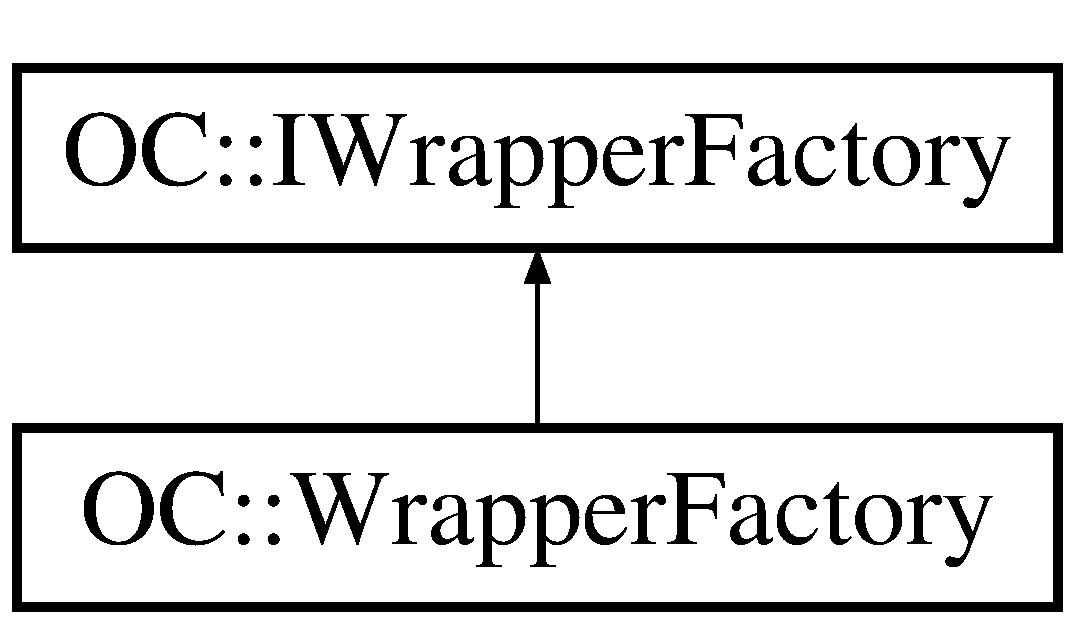
\includegraphics[height=2.000000cm]{classOC_1_1WrapperFactory}
\end{center}
\end{figure}
\subsection*{Public Member Functions}
\begin{DoxyCompactItemize}
\item 
\hypertarget{classOC_1_1WrapperFactory_a6ded2fe20b7eac4adb686ad4abb02508}{}virtual I\+Client\+Wrapper\+::\+Ptr {\bfseries Create\+Client\+Wrapper} (std\+::weak\+\_\+ptr$<$ std\+::mutex $>$ csdk\+Lock, \hyperlink{structOC_1_1PlatformConfig}{Platform\+Config} cfg)\label{classOC_1_1WrapperFactory_a6ded2fe20b7eac4adb686ad4abb02508}

\item 
\hypertarget{classOC_1_1WrapperFactory_a82b951f3b46b68fc2726f41a248c9c32}{}virtual I\+Server\+Wrapper\+::\+Ptr {\bfseries Create\+Server\+Wrapper} (std\+::weak\+\_\+ptr$<$ std\+::mutex $>$ csdk\+Lock, \hyperlink{structOC_1_1PlatformConfig}{Platform\+Config} cfg)\label{classOC_1_1WrapperFactory_a82b951f3b46b68fc2726f41a248c9c32}

\end{DoxyCompactItemize}
\subsection*{Additional Inherited Members}


The documentation for this class was generated from the following file\+:\begin{DoxyCompactItemize}
\item 
/home/user/\+O\+I\+C/oic-\/resource/include/Wrapper\+Factory.\+h\end{DoxyCompactItemize}

\chapter{File Documentation}
\hypertarget{address_8h}{}\section{/home/user/\+O\+I\+C/oic-\/resource/csdk/libcoap-\/4.1.1/address.h File Reference}
\label{address_8h}\index{/home/user/\+O\+I\+C/oic-\/resource/csdk/libcoap-\/4.\+1.\+1/address.\+h@{/home/user/\+O\+I\+C/oic-\/resource/csdk/libcoap-\/4.\+1.\+1/address.\+h}}


representation of network addresses  


{\ttfamily \#include \char`\"{}config.\+h\char`\"{}}\\*
{\ttfamily \#include $<$assert.\+h$>$}\\*
{\ttfamily \#include $<$string.\+h$>$}\\*
{\ttfamily \#include $<$stdint.\+h$>$}\\*
{\ttfamily \#include \char`\"{}ocsocket.\+h\char`\"{}}\\*
{\ttfamily \#include $<$netinet/in.\+h$>$}\\*
{\ttfamily \#include $<$sys/socket.\+h$>$}\\*


\subsection{Detailed Description}
representation of network addresses 


\hypertarget{async_8h}{}\section{/home/user/\+O\+I\+C/oic-\/resource/csdk/libcoap-\/4.1.1/async.h File Reference}
\label{async_8h}\index{/home/user/\+O\+I\+C/oic-\/resource/csdk/libcoap-\/4.\+1.\+1/async.\+h@{/home/user/\+O\+I\+C/oic-\/resource/csdk/libcoap-\/4.\+1.\+1/async.\+h}}


state management for asynchronous messages  


{\ttfamily \#include \char`\"{}config.\+h\char`\"{}}\\*
{\ttfamily \#include \char`\"{}net.\+h\char`\"{}}\\*
\subsection*{Classes}
\begin{DoxyCompactItemize}
\item 
struct \hyperlink{structcoap__async__state__t}{coap\+\_\+async\+\_\+state\+\_\+t}
\end{DoxyCompactItemize}
\subsection*{Macros}
\begin{DoxyCompactItemize}
\item 
\#define \hyperlink{group__coap__async_gaf3c112eaa3f262731ed3507a228bf776}{C\+O\+A\+P\+\_\+\+A\+S\+Y\+N\+C\+\_\+\+C\+O\+N\+F\+I\+R\+M}~0x01
\item 
\#define \hyperlink{group__coap__async_ga0e2fc01767b333ad5badc838014049e6}{C\+O\+A\+P\+\_\+\+A\+S\+Y\+N\+C\+\_\+\+S\+E\+P\+A\+R\+A\+T\+E}~0x02
\item 
\#define \hyperlink{group__coap__async_gac7fcd5adcc9fb3cc90ba2ce6695ee6d0}{C\+O\+A\+P\+\_\+\+A\+S\+Y\+N\+C\+\_\+\+O\+B\+S\+E\+R\+V\+E\+D}~0x04
\item 
\#define \hyperlink{group__coap__async_gab13ab4a40fab483ee2eaef1ac39fd1d8}{C\+O\+A\+P\+\_\+\+A\+S\+Y\+N\+C\+\_\+\+R\+E\+L\+E\+A\+S\+E\+\_\+\+D\+A\+T\+A}~0x08
\end{DoxyCompactItemize}
\subsection*{Typedefs}
\begin{DoxyCompactItemize}
\item 
\hypertarget{group__coap__async_ga6e8319b71d55c3d7fb4dcfc7d5cab3ed}{}typedef struct \hyperlink{structcoap__async__state__t}{coap\+\_\+async\+\_\+state\+\_\+t} {\bfseries coap\+\_\+async\+\_\+state\+\_\+t}\label{group__coap__async_ga6e8319b71d55c3d7fb4dcfc7d5cab3ed}

\end{DoxyCompactItemize}
\subsection*{Functions}
\begin{DoxyCompactItemize}
\item 
\hyperlink{structcoap__async__state__t}{coap\+\_\+async\+\_\+state\+\_\+t} $\ast$ \hyperlink{group__coap__async_ga1c81eb1d464e9b5195acb7ae630e15c9}{coap\+\_\+register\+\_\+async} (\hyperlink{structcoap__context__t}{coap\+\_\+context\+\_\+t} $\ast$context, coap\+\_\+address\+\_\+t $\ast$peer, \hyperlink{structcoap__pdu__t}{coap\+\_\+pdu\+\_\+t} $\ast$request, unsigned char flags, void $\ast$data)
\item 
int \hyperlink{group__coap__async_ga5ebdd339b85d066d741adf64ce51fe0b}{coap\+\_\+remove\+\_\+async} (\hyperlink{structcoap__context__t}{coap\+\_\+context\+\_\+t} $\ast$context, coap\+\_\+tid\+\_\+t id, \hyperlink{structcoap__async__state__t}{coap\+\_\+async\+\_\+state\+\_\+t} $\ast$$\ast$s)
\item 
void \hyperlink{group__coap__async_ga32024a34a383832e6692d3a439fc67c7}{coap\+\_\+free\+\_\+async} (\hyperlink{structcoap__async__state__t}{coap\+\_\+async\+\_\+state\+\_\+t} $\ast$state)
\item 
\hyperlink{structcoap__async__state__t}{coap\+\_\+async\+\_\+state\+\_\+t} $\ast$ \hyperlink{group__coap__async_ga3c064a99c809502d8b584dbbd0d96bd2}{coap\+\_\+find\+\_\+async} (\hyperlink{structcoap__context__t}{coap\+\_\+context\+\_\+t} $\ast$context, coap\+\_\+tid\+\_\+t id)
\end{DoxyCompactItemize}


\subsection{Detailed Description}
state management for asynchronous messages 


\hypertarget{bits_8h}{}\section{/home/user/\+O\+I\+C/oic-\/resource/csdk/libcoap-\/4.1.1/bits.h File Reference}
\label{bits_8h}\index{/home/user/\+O\+I\+C/oic-\/resource/csdk/libcoap-\/4.\+1.\+1/bits.\+h@{/home/user/\+O\+I\+C/oic-\/resource/csdk/libcoap-\/4.\+1.\+1/bits.\+h}}


bit vector manipulation  


{\ttfamily \#include $<$sys/types.\+h$>$}\\*
{\ttfamily \#include $<$stdint.\+h$>$}\\*


\subsection{Detailed Description}
bit vector manipulation 


\hypertarget{coap__time_8h}{}\section{/home/user/\+O\+I\+C/oic-\/resource/csdk/libcoap-\/4.1.1/coap\+\_\+time.h File Reference}
\label{coap__time_8h}\index{/home/user/\+O\+I\+C/oic-\/resource/csdk/libcoap-\/4.\+1.\+1/coap\+\_\+time.\+h@{/home/user/\+O\+I\+C/oic-\/resource/csdk/libcoap-\/4.\+1.\+1/coap\+\_\+time.\+h}}


Clock Handling.  


{\ttfamily \#include \char`\"{}config.\+h\char`\"{}}\\*
\subsection*{Macros}
\begin{DoxyCompactItemize}
\item 
\hypertarget{group__clock_ga30cc030c56bca3f2420e671e0650ca69}{}\#define {\bfseries coap\+\_\+clock\+\_\+init}~coap\+\_\+clock\+\_\+init\+\_\+impl\label{group__clock_ga30cc030c56bca3f2420e671e0650ca69}

\item 
\hypertarget{group__clock_gaeacdaf84024e9c066fb5c37e82dc1f17}{}\#define {\bfseries coap\+\_\+ticks}~coap\+\_\+ticks\+\_\+impl\label{group__clock_gaeacdaf84024e9c066fb5c37e82dc1f17}

\end{DoxyCompactItemize}


\subsection{Detailed Description}
Clock Handling. 


\hypertarget{hashkey_8h}{}\section{/home/user/\+O\+I\+C/oic-\/resource/csdk/libcoap-\/4.1.1/hashkey.h File Reference}
\label{hashkey_8h}\index{/home/user/\+O\+I\+C/oic-\/resource/csdk/libcoap-\/4.\+1.\+1/hashkey.\+h@{/home/user/\+O\+I\+C/oic-\/resource/csdk/libcoap-\/4.\+1.\+1/hashkey.\+h}}


definition of hash key type and helper functions  


{\ttfamily \#include \char`\"{}str.\+h\char`\"{}}\\*
\subsection*{Macros}
\begin{DoxyCompactItemize}
\item 
\hypertarget{hashkey_8h_a7367053289edae33b9f02771d89b0ffa}{}\#define {\bfseries coap\+\_\+hash}(String,  Length,  Result)~\hyperlink{hashkey_8h_a1f8fb366d21f56f2e619c42a516114f6}{coap\+\_\+hash\+\_\+impl}((String),(Length),(Result))\label{hashkey_8h_a7367053289edae33b9f02771d89b0ffa}

\item 
\hypertarget{hashkey_8h_adbcef676b65aa7e7f30b0f141732c4af}{}\#define {\bfseries \+\_\+\+\_\+\+C\+O\+A\+P\+\_\+\+D\+E\+F\+A\+U\+L\+T\+\_\+\+H\+A\+S\+H}\label{hashkey_8h_adbcef676b65aa7e7f30b0f141732c4af}

\item 
\#define \hyperlink{hashkey_8h_aab841b0811b13cfb044f82718114b196}{coap\+\_\+str\+\_\+hash}(Str,  H)
\end{DoxyCompactItemize}
\subsection*{Typedefs}
\begin{DoxyCompactItemize}
\item 
\hypertarget{hashkey_8h_a14b49ce1f8be4059e84df8e9d2a19586}{}typedef unsigned char {\bfseries coap\+\_\+key\+\_\+t}\mbox{[}4\mbox{]}\label{hashkey_8h_a14b49ce1f8be4059e84df8e9d2a19586}

\end{DoxyCompactItemize}
\subsection*{Functions}
\begin{DoxyCompactItemize}
\item 
void \hyperlink{hashkey_8h_a1f8fb366d21f56f2e619c42a516114f6}{coap\+\_\+hash\+\_\+impl} (const unsigned char $\ast$s, unsigned int len, coap\+\_\+key\+\_\+t h)
\end{DoxyCompactItemize}


\subsection{Detailed Description}
definition of hash key type and helper functions 



\subsection{Macro Definition Documentation}
\hypertarget{hashkey_8h_aab841b0811b13cfb044f82718114b196}{}\index{hashkey.\+h@{hashkey.\+h}!coap\+\_\+str\+\_\+hash@{coap\+\_\+str\+\_\+hash}}
\index{coap\+\_\+str\+\_\+hash@{coap\+\_\+str\+\_\+hash}!hashkey.\+h@{hashkey.\+h}}
\subsubsection[{coap\+\_\+str\+\_\+hash}]{\setlength{\rightskip}{0pt plus 5cm}\#define coap\+\_\+str\+\_\+hash(
\begin{DoxyParamCaption}
\item[{}]{Str, }
\item[{}]{H}
\end{DoxyParamCaption}
)}\label{hashkey_8h_aab841b0811b13cfb044f82718114b196}
Calls coap\+\_\+hash() with given {\ttfamily str} object as parameter.


\begin{DoxyParams}{Parameters}
{\em Str} & Must contain a pointer to a coap string object. \\
\hline
{\em H} & A coap\+\_\+key\+\_\+t object to store the result. \\
\hline
\end{DoxyParams}


\subsection{Function Documentation}
\hypertarget{hashkey_8h_a1f8fb366d21f56f2e619c42a516114f6}{}\index{hashkey.\+h@{hashkey.\+h}!coap\+\_\+hash\+\_\+impl@{coap\+\_\+hash\+\_\+impl}}
\index{coap\+\_\+hash\+\_\+impl@{coap\+\_\+hash\+\_\+impl}!hashkey.\+h@{hashkey.\+h}}
\subsubsection[{coap\+\_\+hash\+\_\+impl}]{\setlength{\rightskip}{0pt plus 5cm}void coap\+\_\+hash\+\_\+impl (
\begin{DoxyParamCaption}
\item[{const unsigned char $\ast$}]{s, }
\item[{unsigned int}]{len, }
\item[{coap\+\_\+key\+\_\+t}]{h}
\end{DoxyParamCaption}
)}\label{hashkey_8h_a1f8fb366d21f56f2e619c42a516114f6}
Calculates a fast hash over the given string {\ttfamily s} of length {\ttfamily len} and stores the result into {\ttfamily h}. Depending on the exact implementation, this function cannot be used as one-\/way function to check message integrity or simlar.


\begin{DoxyParams}{Parameters}
{\em s} & The string used for hash calculation. \\
\hline
{\em len} & The length of {\ttfamily s}. \\
\hline
{\em h} & The result buffer to store the calculated hash key. \\
\hline
\end{DoxyParams}

\hypertarget{option_8h}{}\section{/home/user/\+O\+I\+C/oic-\/resource/csdk/libcoap-\/4.1.1/option.h File Reference}
\label{option_8h}\index{/home/user/\+O\+I\+C/oic-\/resource/csdk/libcoap-\/4.\+1.\+1/option.\+h@{/home/user/\+O\+I\+C/oic-\/resource/csdk/libcoap-\/4.\+1.\+1/option.\+h}}


helpers for handling options in Co\+A\+P P\+D\+Us  


{\ttfamily \#include \char`\"{}bits.\+h\char`\"{}}\\*
{\ttfamily \#include \char`\"{}pdu.\+h\char`\"{}}\\*
\subsection*{Classes}
\begin{DoxyCompactItemize}
\item 
struct \hyperlink{structcoap__option__t}{coap\+\_\+option\+\_\+t}
\item 
struct \hyperlink{structcoap__opt__iterator__t}{coap\+\_\+opt\+\_\+iterator\+\_\+t}
\end{DoxyCompactItemize}
\subsection*{Macros}
\begin{DoxyCompactItemize}
\item 
\hypertarget{option_8h_a4d26009eb308f3867747b0aa713a1755}{}\#define {\bfseries P\+C\+H\+A\+R}(p)~((\hyperlink{option_8h_a351867e79474c96130f738fcfbc120cc}{coap\+\_\+opt\+\_\+t} $\ast$)(p))\label{option_8h_a4d26009eb308f3867747b0aa713a1755}

\item 
\#define \hyperlink{option_8h_a099224ae51d2b85fb4cbeb5f07ce52f7}{C\+O\+A\+P\+\_\+\+O\+P\+T\+\_\+\+S\+I\+Z\+E}(opt)~\hyperlink{option_8h_a683c0121b4028a90f612809437aaa3d0}{coap\+\_\+opt\+\_\+size}(opt)
\item 
\#define \hyperlink{option_8h_a9131d506cda7061edb855e65d796d6da}{options\+\_\+next}(opt)
\item 
\#define \hyperlink{group__opt__filter_ga81f470e9cdcc258799e10f6ed8a3ce5e}{C\+O\+A\+P\+\_\+\+O\+P\+T\+\_\+\+A\+L\+L}~N\+U\+L\+L
\item 
\#define \hyperlink{group__opt__filter_ga40b8b72ce87dcece9185a0911ec2c588}{C\+O\+A\+P\+\_\+\+O\+P\+T\+\_\+\+D\+E\+L\+T\+A}(opt)~\hyperlink{group__opt__filter_gacec6795999a3ddaa56025a70abdc1d38}{coap\+\_\+opt\+\_\+delta}(opt)
\item 
\#define \hyperlink{group__opt__filter_ga2abe054935d45806d901a90ce5c4bd5d}{C\+O\+A\+P\+\_\+\+O\+P\+T\+\_\+\+S\+E\+T\+D\+E\+L\+T\+A}(opt,  val)~\hyperlink{group__opt__filter_ga8b601ead68a35f2bcca8c101b0b93c23}{coap\+\_\+opt\+\_\+encode}((opt), C\+O\+A\+P\+\_\+\+M\+A\+X\+\_\+\+P\+D\+U\+\_\+\+S\+I\+Z\+E, (val), N\+U\+L\+L, 0)
\item 
\#define \hyperlink{group__opt__filter_gad8982f51d2fb676d4b4be50487bb8590}{C\+O\+A\+P\+\_\+\+O\+P\+T\+\_\+\+L\+E\+N\+G\+T\+H}(opt)~\hyperlink{group__opt__filter_ga5616c72178d923fb02db863c87ee249f}{coap\+\_\+opt\+\_\+length}(opt)
\item 
\#define \hyperlink{group__opt__filter_gac4348d760bb312fdc2f108ee3e8303a4}{C\+O\+A\+P\+\_\+\+O\+P\+T\+\_\+\+V\+A\+L\+U\+E}(opt)~\hyperlink{group__opt__filter_ga0f80e7bb12dca927fdf5829804c84b0e}{coap\+\_\+opt\+\_\+value}((\hyperlink{option_8h_a351867e79474c96130f738fcfbc120cc}{coap\+\_\+opt\+\_\+t} $\ast$)opt)
\end{DoxyCompactItemize}
\subsection*{Typedefs}
\begin{DoxyCompactItemize}
\item 
typedef unsigned char \hyperlink{option_8h_a351867e79474c96130f738fcfbc120cc}{coap\+\_\+opt\+\_\+t}
\item 
typedef unsigned char \hyperlink{group__opt__filter_gace614f18a4f0133a72096094c11c3b19}{coap\+\_\+opt\+\_\+filter\+\_\+t}\mbox{[}(C\+O\+A\+P\+\_\+\+M\+A\+X\+\_\+\+O\+P\+T $>$$>$ 3)+1\mbox{]}
\end{DoxyCompactItemize}
\subsection*{Functions}
\begin{DoxyCompactItemize}
\item 
size\+\_\+t \hyperlink{option_8h_a11de99f50cc9f5a34fd9e4d121ecfd13}{coap\+\_\+opt\+\_\+parse} (const \hyperlink{option_8h_a351867e79474c96130f738fcfbc120cc}{coap\+\_\+opt\+\_\+t} $\ast$opt, size\+\_\+t length, \hyperlink{structcoap__option__t}{coap\+\_\+option\+\_\+t} $\ast$result)
\item 
size\+\_\+t \hyperlink{option_8h_a683c0121b4028a90f612809437aaa3d0}{coap\+\_\+opt\+\_\+size} (const \hyperlink{option_8h_a351867e79474c96130f738fcfbc120cc}{coap\+\_\+opt\+\_\+t} $\ast$opt)
\item 
\hyperlink{option_8h_a351867e79474c96130f738fcfbc120cc}{coap\+\_\+opt\+\_\+t} $\ast$ \hyperlink{option_8h_a7c2dec4ec740abfeafc695114602d1cd}{options\+\_\+start} (\hyperlink{structcoap__pdu__t}{coap\+\_\+pdu\+\_\+t} $\ast$pdu)
\item 
\hyperlink{structcoap__opt__iterator__t}{coap\+\_\+opt\+\_\+iterator\+\_\+t} $\ast$ \hyperlink{group__opt__filter_gacec8f143e7a4fe66d97f719f619d42b3}{coap\+\_\+option\+\_\+iterator\+\_\+init} (\hyperlink{structcoap__pdu__t}{coap\+\_\+pdu\+\_\+t} $\ast$pdu, \hyperlink{structcoap__opt__iterator__t}{coap\+\_\+opt\+\_\+iterator\+\_\+t} $\ast$oi, const \hyperlink{group__opt__filter_gace614f18a4f0133a72096094c11c3b19}{coap\+\_\+opt\+\_\+filter\+\_\+t} filter)
\item 
\hyperlink{option_8h_a351867e79474c96130f738fcfbc120cc}{coap\+\_\+opt\+\_\+t} $\ast$ \hyperlink{group__opt__filter_ga182fdeffe0b37e1ab0dc6ba8494abe4a}{coap\+\_\+option\+\_\+next} (\hyperlink{structcoap__opt__iterator__t}{coap\+\_\+opt\+\_\+iterator\+\_\+t} $\ast$oi)
\item 
\hyperlink{option_8h_a351867e79474c96130f738fcfbc120cc}{coap\+\_\+opt\+\_\+t} $\ast$ \hyperlink{group__opt__filter_gab2a1a3719d25b39377063c7cebac258d}{coap\+\_\+check\+\_\+option} (\hyperlink{structcoap__pdu__t}{coap\+\_\+pdu\+\_\+t} $\ast$pdu, unsigned char type, \hyperlink{structcoap__opt__iterator__t}{coap\+\_\+opt\+\_\+iterator\+\_\+t} $\ast$oi)
\item 
size\+\_\+t \hyperlink{group__opt__filter_ga6cc876020a0017266ffea98e949073dc}{coap\+\_\+opt\+\_\+setheader} (\hyperlink{option_8h_a351867e79474c96130f738fcfbc120cc}{coap\+\_\+opt\+\_\+t} $\ast$opt, size\+\_\+t maxlen, unsigned short delta, size\+\_\+t length)
\item 
size\+\_\+t \hyperlink{group__opt__filter_ga8b601ead68a35f2bcca8c101b0b93c23}{coap\+\_\+opt\+\_\+encode} (\hyperlink{option_8h_a351867e79474c96130f738fcfbc120cc}{coap\+\_\+opt\+\_\+t} $\ast$opt, size\+\_\+t n, unsigned short delta, const unsigned char $\ast$val, size\+\_\+t length)
\item 
unsigned short \hyperlink{group__opt__filter_gacec6795999a3ddaa56025a70abdc1d38}{coap\+\_\+opt\+\_\+delta} (const \hyperlink{option_8h_a351867e79474c96130f738fcfbc120cc}{coap\+\_\+opt\+\_\+t} $\ast$opt)
\item 
unsigned short \hyperlink{group__opt__filter_ga5616c72178d923fb02db863c87ee249f}{coap\+\_\+opt\+\_\+length} (const \hyperlink{option_8h_a351867e79474c96130f738fcfbc120cc}{coap\+\_\+opt\+\_\+t} $\ast$opt)
\item 
unsigned char $\ast$ \hyperlink{group__opt__filter_ga0f80e7bb12dca927fdf5829804c84b0e}{coap\+\_\+opt\+\_\+value} (\hyperlink{option_8h_a351867e79474c96130f738fcfbc120cc}{coap\+\_\+opt\+\_\+t} $\ast$opt)
\end{DoxyCompactItemize}


\subsection{Detailed Description}
helpers for handling options in Co\+A\+P P\+D\+Us 



\subsection{Macro Definition Documentation}
\hypertarget{option_8h_a099224ae51d2b85fb4cbeb5f07ce52f7}{}\index{option.\+h@{option.\+h}!C\+O\+A\+P\+\_\+\+O\+P\+T\+\_\+\+S\+I\+Z\+E@{C\+O\+A\+P\+\_\+\+O\+P\+T\+\_\+\+S\+I\+Z\+E}}
\index{C\+O\+A\+P\+\_\+\+O\+P\+T\+\_\+\+S\+I\+Z\+E@{C\+O\+A\+P\+\_\+\+O\+P\+T\+\_\+\+S\+I\+Z\+E}!option.\+h@{option.\+h}}
\subsubsection[{C\+O\+A\+P\+\_\+\+O\+P\+T\+\_\+\+S\+I\+Z\+E}]{\setlength{\rightskip}{0pt plus 5cm}\#define C\+O\+A\+P\+\_\+\+O\+P\+T\+\_\+\+S\+I\+Z\+E(
\begin{DoxyParamCaption}
\item[{}]{opt}
\end{DoxyParamCaption}
)~{\bf coap\+\_\+opt\+\_\+size}(opt)}\label{option_8h_a099224ae51d2b85fb4cbeb5f07ce52f7}
\begin{DoxyRefDesc}{Deprecated}
\item[\hyperlink{deprecated__deprecated000001}{Deprecated}]\{ Use \hyperlink{option_8h_a683c0121b4028a90f612809437aaa3d0}{coap\+\_\+opt\+\_\+size()} instead. \} \end{DoxyRefDesc}
\hypertarget{option_8h_a9131d506cda7061edb855e65d796d6da}{}\index{option.\+h@{option.\+h}!options\+\_\+next@{options\+\_\+next}}
\index{options\+\_\+next@{options\+\_\+next}!option.\+h@{option.\+h}}
\subsubsection[{options\+\_\+next}]{\setlength{\rightskip}{0pt plus 5cm}\#define options\+\_\+next(
\begin{DoxyParamCaption}
\item[{}]{opt}
\end{DoxyParamCaption}
)}\label{option_8h_a9131d506cda7061edb855e65d796d6da}
Interprets {\ttfamily opt} as pointer to a Co\+A\+P option and advances to the next byte past this option. 

\subsection{Typedef Documentation}
\hypertarget{option_8h_a351867e79474c96130f738fcfbc120cc}{}\index{option.\+h@{option.\+h}!coap\+\_\+opt\+\_\+t@{coap\+\_\+opt\+\_\+t}}
\index{coap\+\_\+opt\+\_\+t@{coap\+\_\+opt\+\_\+t}!option.\+h@{option.\+h}}
\subsubsection[{coap\+\_\+opt\+\_\+t}]{\setlength{\rightskip}{0pt plus 5cm}typedef unsigned char {\bf coap\+\_\+opt\+\_\+t}}\label{option_8h_a351867e79474c96130f738fcfbc120cc}
Use byte-\/oriented access methods here because sliding a complex struct coap\+\_\+opt\+\_\+t over the data buffer may cause bus error on certain platforms. 

\subsection{Function Documentation}
\hypertarget{option_8h_a11de99f50cc9f5a34fd9e4d121ecfd13}{}\index{option.\+h@{option.\+h}!coap\+\_\+opt\+\_\+parse@{coap\+\_\+opt\+\_\+parse}}
\index{coap\+\_\+opt\+\_\+parse@{coap\+\_\+opt\+\_\+parse}!option.\+h@{option.\+h}}
\subsubsection[{coap\+\_\+opt\+\_\+parse}]{\setlength{\rightskip}{0pt plus 5cm}size\+\_\+t coap\+\_\+opt\+\_\+parse (
\begin{DoxyParamCaption}
\item[{const {\bf coap\+\_\+opt\+\_\+t} $\ast$}]{opt, }
\item[{size\+\_\+t}]{length, }
\item[{{\bf coap\+\_\+option\+\_\+t} $\ast$}]{result}
\end{DoxyParamCaption}
)}\label{option_8h_a11de99f50cc9f5a34fd9e4d121ecfd13}
Parses the option pointed to by {\ttfamily opt} into {\ttfamily result}. This function returns the number of bytes that have been parsed, or {\ttfamily 0} on error. An error is signaled when illegal delta or length values are encountered or when option parsing would result in reading past the option (i.\+e. beyond opt + length).


\begin{DoxyParams}{Parameters}
{\em opt} & The beginning of the option to parse. \\
\hline
{\em length} & The maximum length of {\ttfamily opt}. \\
\hline
{\em result} & A pointer to the \hyperlink{structcoap__option__t}{coap\+\_\+option\+\_\+t} structure that is filled with actual values iff \hyperlink{option_8h_a11de99f50cc9f5a34fd9e4d121ecfd13}{coap\+\_\+opt\+\_\+parse()} $>$ 0. \\
\hline
\end{DoxyParams}
\begin{DoxyReturn}{Returns}
The number of bytes parsed or {\ttfamily 0} on error. 
\end{DoxyReturn}
\hypertarget{option_8h_a683c0121b4028a90f612809437aaa3d0}{}\index{option.\+h@{option.\+h}!coap\+\_\+opt\+\_\+size@{coap\+\_\+opt\+\_\+size}}
\index{coap\+\_\+opt\+\_\+size@{coap\+\_\+opt\+\_\+size}!option.\+h@{option.\+h}}
\subsubsection[{coap\+\_\+opt\+\_\+size}]{\setlength{\rightskip}{0pt plus 5cm}size\+\_\+t coap\+\_\+opt\+\_\+size (
\begin{DoxyParamCaption}
\item[{const {\bf coap\+\_\+opt\+\_\+t} $\ast$}]{opt}
\end{DoxyParamCaption}
)}\label{option_8h_a683c0121b4028a90f612809437aaa3d0}
Returns the size of the given option, taking into account a possible option jump.


\begin{DoxyParams}{Parameters}
{\em opt} & An option jump or the beginning of the option. \\
\hline
\end{DoxyParams}
\begin{DoxyReturn}{Returns}
The number of bytes between {\ttfamily opt} and the end of the option starting at {\ttfamily opt}. In case of an error, this function returns {\ttfamily 0} as options need at least one byte storage space. 
\end{DoxyReturn}
\hypertarget{option_8h_a7c2dec4ec740abfeafc695114602d1cd}{}\index{option.\+h@{option.\+h}!options\+\_\+start@{options\+\_\+start}}
\index{options\+\_\+start@{options\+\_\+start}!option.\+h@{option.\+h}}
\subsubsection[{options\+\_\+start}]{\setlength{\rightskip}{0pt plus 5cm}{\bf coap\+\_\+opt\+\_\+t}$\ast$ options\+\_\+start (
\begin{DoxyParamCaption}
\item[{{\bf coap\+\_\+pdu\+\_\+t} $\ast$}]{pdu}
\end{DoxyParamCaption}
)}\label{option_8h_a7c2dec4ec740abfeafc695114602d1cd}
Calculates the beginning of the P\+D\+U's option section.


\begin{DoxyParams}{Parameters}
{\em pdu} & The P\+D\+U containing the options. \\
\hline
\end{DoxyParams}
\begin{DoxyReturn}{Returns}
A pointer to the first option if available, or {\ttfamily N\+U\+L\+L} otherwise. 
\end{DoxyReturn}

\hypertarget{prng_8h}{}\section{/home/user/\+O\+I\+C/oic-\/resource/csdk/libcoap-\/4.1.1/prng.h File Reference}
\label{prng_8h}\index{/home/user/\+O\+I\+C/oic-\/resource/csdk/libcoap-\/4.\+1.\+1/prng.\+h@{/home/user/\+O\+I\+C/oic-\/resource/csdk/libcoap-\/4.\+1.\+1/prng.\+h}}


Pseudo Random Numbers.  


{\ttfamily \#include \char`\"{}config.\+h\char`\"{}}\\*
{\ttfamily \#include $<$ocrandom.\+h$>$}\\*
{\ttfamily \#include $<$stdlib.\+h$>$}\\*
\subsection*{Macros}
\begin{DoxyCompactItemize}
\item 
\#define \hyperlink{group__prng_ga7c7d6401e43c811dacb517d51184c873}{prng}(Buf,  Length)
\item 
\#define \hyperlink{group__prng_gaa32e46211968b5a4936d4c122b7fd44c}{prng\+\_\+init}(Value)
\end{DoxyCompactItemize}


\subsection{Detailed Description}
Pseudo Random Numbers. 


\hypertarget{resource_8h}{}\section{/home/user/\+O\+I\+C/oic-\/resource/csdk/libcoap-\/4.1.1/resource.h File Reference}
\label{resource_8h}\index{/home/user/\+O\+I\+C/oic-\/resource/csdk/libcoap-\/4.\+1.\+1/resource.\+h@{/home/user/\+O\+I\+C/oic-\/resource/csdk/libcoap-\/4.\+1.\+1/resource.\+h}}


generic resource handling  


{\ttfamily \#include \char`\"{}config.\+h\char`\"{}}\\*
{\ttfamily \#include \char`\"{}t\+\_\+list.\+h\char`\"{}}\\*
{\ttfamily \#include \char`\"{}async.\+h\char`\"{}}\\*
{\ttfamily \#include $<$assert.\+h$>$}\\*
{\ttfamily \#include \char`\"{}uthash.\+h\char`\"{}}\\*
{\ttfamily \#include \char`\"{}hashkey.\+h\char`\"{}}\\*
{\ttfamily \#include \char`\"{}str.\+h\char`\"{}}\\*
{\ttfamily \#include \char`\"{}pdu.\+h\char`\"{}}\\*
{\ttfamily \#include \char`\"{}net.\+h\char`\"{}}\\*
{\ttfamily \#include \char`\"{}subscribe.\+h\char`\"{}}\\*
\subsection*{Classes}
\begin{DoxyCompactItemize}
\item 
struct \hyperlink{structcoap__attr__t}{coap\+\_\+attr\+\_\+t}
\item 
struct \hyperlink{structcoap__resource__t}{coap\+\_\+resource\+\_\+t}
\end{DoxyCompactItemize}
\subsection*{Macros}
\begin{DoxyCompactItemize}
\item 
\#define \hyperlink{resource_8h_a8d07061a1bb4a55b64c517b5a0a02914}{C\+O\+A\+P\+\_\+\+R\+E\+S\+O\+U\+R\+C\+E\+\_\+\+C\+H\+E\+C\+K\+\_\+\+T\+I\+M\+E}~2
\item 
\hypertarget{resource_8h_a2892686485c67ab0b946708ad59bcf51}{}\#define {\bfseries C\+O\+A\+P\+\_\+\+A\+T\+T\+R\+\_\+\+F\+L\+A\+G\+S\+\_\+\+R\+E\+L\+E\+A\+S\+E\+\_\+\+N\+A\+M\+E}~0x1\label{resource_8h_a2892686485c67ab0b946708ad59bcf51}

\item 
\hypertarget{resource_8h_a1dfff2e71cc242377e92e0b322ddd1ea}{}\#define {\bfseries C\+O\+A\+P\+\_\+\+A\+T\+T\+R\+\_\+\+F\+L\+A\+G\+S\+\_\+\+R\+E\+L\+E\+A\+S\+E\+\_\+\+V\+A\+L\+U\+E}~0x2\label{resource_8h_a1dfff2e71cc242377e92e0b322ddd1ea}

\item 
\hypertarget{resource_8h_aee71da70d15897c276b0c4166ad1eaa6}{}\#define {\bfseries C\+O\+A\+P\+\_\+\+R\+E\+S\+O\+U\+R\+C\+E\+\_\+\+F\+L\+A\+G\+S\+\_\+\+R\+E\+L\+E\+A\+S\+E\+\_\+\+U\+R\+I}~0x1\label{resource_8h_aee71da70d15897c276b0c4166ad1eaa6}

\item 
\hypertarget{resource_8h_a22f2db8593afab3bb8c153e2346fdf75}{}\#define {\bfseries C\+O\+A\+P\+\_\+\+P\+R\+I\+N\+T\+\_\+\+S\+T\+A\+T\+U\+S\+\_\+\+M\+A\+S\+K}~0x\+F0000000u\label{resource_8h_a22f2db8593afab3bb8c153e2346fdf75}

\item 
\hypertarget{resource_8h_acf2fbde3cc54e108713886d6e23040f0}{}\#define {\bfseries C\+O\+A\+P\+\_\+\+P\+R\+I\+N\+T\+\_\+\+O\+U\+T\+P\+U\+T\+\_\+\+L\+E\+N\+G\+T\+H}(v)~((v) \& $\sim$C\+O\+A\+P\+\_\+\+P\+R\+I\+N\+T\+\_\+\+S\+T\+A\+T\+U\+S\+\_\+\+M\+A\+S\+K)\label{resource_8h_acf2fbde3cc54e108713886d6e23040f0}

\item 
\hypertarget{resource_8h_abba955fb8180d86085c2f0680626cfe8}{}\#define {\bfseries C\+O\+A\+P\+\_\+\+P\+R\+I\+N\+T\+\_\+\+S\+T\+A\+T\+U\+S\+\_\+\+E\+R\+R\+O\+R}~0x80000000u\label{resource_8h_abba955fb8180d86085c2f0680626cfe8}

\item 
\hypertarget{resource_8h_a457e1894c102b193d1d59de022035ac9}{}\#define {\bfseries C\+O\+A\+P\+\_\+\+P\+R\+I\+N\+T\+\_\+\+S\+T\+A\+T\+U\+S\+\_\+\+T\+R\+U\+N\+C}~0x40000000u\label{resource_8h_a457e1894c102b193d1d59de022035ac9}

\end{DoxyCompactItemize}
\subsection*{Typedefs}
\begin{DoxyCompactItemize}
\item 
typedef void($\ast$ \hyperlink{resource_8h_ad2b83945efbc3230d64f81d0e966df56}{coap\+\_\+method\+\_\+handler\+\_\+t}) (\hyperlink{structcoap__context__t}{coap\+\_\+context\+\_\+t} $\ast$, struct \hyperlink{structcoap__resource__t}{coap\+\_\+resource\+\_\+t} $\ast$, coap\+\_\+address\+\_\+t $\ast$, \hyperlink{structcoap__pdu__t}{coap\+\_\+pdu\+\_\+t} $\ast$, \hyperlink{structstr}{str} $\ast$, \hyperlink{structcoap__pdu__t}{coap\+\_\+pdu\+\_\+t} $\ast$)
\item 
\hypertarget{resource_8h_ac0f6fd3889980d7c4fa58aeaba8367f9}{}typedef struct \hyperlink{structcoap__attr__t}{coap\+\_\+attr\+\_\+t} {\bfseries coap\+\_\+attr\+\_\+t}\label{resource_8h_ac0f6fd3889980d7c4fa58aeaba8367f9}

\item 
\hypertarget{resource_8h_abeaeb0eb76bbf5bb401da20b27add830}{}typedef struct \hyperlink{structcoap__resource__t}{coap\+\_\+resource\+\_\+t} {\bfseries coap\+\_\+resource\+\_\+t}\label{resource_8h_abeaeb0eb76bbf5bb401da20b27add830}

\item 
typedef unsigned int \hyperlink{resource_8h_a91b02fe05f44f053f50c8d07b03f1f6e}{coap\+\_\+print\+\_\+status\+\_\+t}
\end{DoxyCompactItemize}
\subsection*{Functions}
\begin{DoxyCompactItemize}
\item 
\hyperlink{structcoap__resource__t}{coap\+\_\+resource\+\_\+t} $\ast$ \hyperlink{resource_8h_ab541655395f1fa9e7088af153506d97e}{coap\+\_\+resource\+\_\+init} (const unsigned char $\ast$uri, size\+\_\+t len, int flags)
\item 
void \hyperlink{resource_8h_a9a5f0705912b0a35a3d5764e86b94004}{coap\+\_\+add\+\_\+resource} (\hyperlink{structcoap__context__t}{coap\+\_\+context\+\_\+t} $\ast$context, \hyperlink{structcoap__resource__t}{coap\+\_\+resource\+\_\+t} $\ast$resource)
\item 
int \hyperlink{resource_8h_a2fb1d46ece1dd907128cb407adcf5257}{coap\+\_\+delete\+\_\+resource} (\hyperlink{structcoap__context__t}{coap\+\_\+context\+\_\+t} $\ast$context, coap\+\_\+key\+\_\+t key)
\item 
\hyperlink{structcoap__attr__t}{coap\+\_\+attr\+\_\+t} $\ast$ \hyperlink{resource_8h_acfd5d20f6bb2051696fa20020e4b4868}{coap\+\_\+add\+\_\+attr} (\hyperlink{structcoap__resource__t}{coap\+\_\+resource\+\_\+t} $\ast$resource, const unsigned char $\ast$name, size\+\_\+t nlen, const unsigned char $\ast$val, size\+\_\+t vlen, int flags)
\item 
\hyperlink{structcoap__attr__t}{coap\+\_\+attr\+\_\+t} $\ast$ \hyperlink{resource_8h_a37cf7fb7da22f9a47e11bcbbbaf0e598}{coap\+\_\+find\+\_\+attr} (\hyperlink{structcoap__resource__t}{coap\+\_\+resource\+\_\+t} $\ast$resource, const unsigned char $\ast$name, size\+\_\+t nlen)
\item 
void \hyperlink{resource_8h_a37883d9c8bafdd59fd1bd57dcb82e908}{coap\+\_\+delete\+\_\+attr} (\hyperlink{structcoap__attr__t}{coap\+\_\+attr\+\_\+t} $\ast$attr)
\item 
\hyperlink{resource_8h_a91b02fe05f44f053f50c8d07b03f1f6e}{coap\+\_\+print\+\_\+status\+\_\+t} \hyperlink{resource_8h_a1ee72943df541ed5d4294c13e967ef09}{coap\+\_\+print\+\_\+link} (const \hyperlink{structcoap__resource__t}{coap\+\_\+resource\+\_\+t} $\ast$resource, unsigned char $\ast$buf, size\+\_\+t $\ast$len, size\+\_\+t $\ast$offset)
\item 
\hyperlink{structcoap__resource__t}{coap\+\_\+resource\+\_\+t} $\ast$ \hyperlink{resource_8h_a0404016926e5d93a5124adf32533bf4b}{coap\+\_\+get\+\_\+resource\+\_\+from\+\_\+key} (\hyperlink{structcoap__context__t}{coap\+\_\+context\+\_\+t} $\ast$context, coap\+\_\+key\+\_\+t key)
\item 
void \hyperlink{resource_8h_a5cd67cb7b62f8e0e74c81fd722cc614d}{coap\+\_\+hash\+\_\+request\+\_\+uri} (const \hyperlink{structcoap__pdu__t}{coap\+\_\+pdu\+\_\+t} $\ast$request, coap\+\_\+key\+\_\+t key)
\item 
\hyperlink{structcoap__subscription__t}{coap\+\_\+subscription\+\_\+t} $\ast$ \hyperlink{resource_8h_a56711b69b4a575e91469899e2bf5fc38}{coap\+\_\+add\+\_\+observer} (\hyperlink{structcoap__resource__t}{coap\+\_\+resource\+\_\+t} $\ast$resource, const coap\+\_\+address\+\_\+t $\ast$observer, const \hyperlink{structstr}{str} $\ast$token)
\item 
\hyperlink{structcoap__subscription__t}{coap\+\_\+subscription\+\_\+t} $\ast$ \hyperlink{resource_8h_aac17b56e9ac858cab28be0121e82abb9}{coap\+\_\+find\+\_\+observer} (\hyperlink{structcoap__resource__t}{coap\+\_\+resource\+\_\+t} $\ast$resource, const coap\+\_\+address\+\_\+t $\ast$peer, const \hyperlink{structstr}{str} $\ast$token)
\item 
void \hyperlink{resource_8h_a763b438391c8d7bfdbfe6b41ab48c3e3}{coap\+\_\+touch\+\_\+observer} (\hyperlink{structcoap__context__t}{coap\+\_\+context\+\_\+t} $\ast$context, const coap\+\_\+address\+\_\+t $\ast$observer, const \hyperlink{structstr}{str} $\ast$token)
\item 
void \hyperlink{resource_8h_a5ae341f151b1e01345c5c5d5144db5a2}{coap\+\_\+delete\+\_\+observer} (\hyperlink{structcoap__resource__t}{coap\+\_\+resource\+\_\+t} $\ast$resource, const coap\+\_\+address\+\_\+t $\ast$observer, const \hyperlink{structstr}{str} $\ast$token)
\item 
void \hyperlink{resource_8h_a579bcb559463d3a872831c18d8d9a1c1}{coap\+\_\+check\+\_\+notify} (\hyperlink{structcoap__context__t}{coap\+\_\+context\+\_\+t} $\ast$context)
\end{DoxyCompactItemize}


\subsection{Detailed Description}
generic resource handling 



\subsection{Macro Definition Documentation}
\hypertarget{resource_8h_a8d07061a1bb4a55b64c517b5a0a02914}{}\index{resource.\+h@{resource.\+h}!C\+O\+A\+P\+\_\+\+R\+E\+S\+O\+U\+R\+C\+E\+\_\+\+C\+H\+E\+C\+K\+\_\+\+T\+I\+M\+E@{C\+O\+A\+P\+\_\+\+R\+E\+S\+O\+U\+R\+C\+E\+\_\+\+C\+H\+E\+C\+K\+\_\+\+T\+I\+M\+E}}
\index{C\+O\+A\+P\+\_\+\+R\+E\+S\+O\+U\+R\+C\+E\+\_\+\+C\+H\+E\+C\+K\+\_\+\+T\+I\+M\+E@{C\+O\+A\+P\+\_\+\+R\+E\+S\+O\+U\+R\+C\+E\+\_\+\+C\+H\+E\+C\+K\+\_\+\+T\+I\+M\+E}!resource.\+h@{resource.\+h}}
\subsubsection[{C\+O\+A\+P\+\_\+\+R\+E\+S\+O\+U\+R\+C\+E\+\_\+\+C\+H\+E\+C\+K\+\_\+\+T\+I\+M\+E}]{\setlength{\rightskip}{0pt plus 5cm}\#define C\+O\+A\+P\+\_\+\+R\+E\+S\+O\+U\+R\+C\+E\+\_\+\+C\+H\+E\+C\+K\+\_\+\+T\+I\+M\+E~2}\label{resource_8h_a8d07061a1bb4a55b64c517b5a0a02914}
The interval in seconds to check if resources have changed. 

\subsection{Typedef Documentation}
\hypertarget{resource_8h_ad2b83945efbc3230d64f81d0e966df56}{}\index{resource.\+h@{resource.\+h}!coap\+\_\+method\+\_\+handler\+\_\+t@{coap\+\_\+method\+\_\+handler\+\_\+t}}
\index{coap\+\_\+method\+\_\+handler\+\_\+t@{coap\+\_\+method\+\_\+handler\+\_\+t}!resource.\+h@{resource.\+h}}
\subsubsection[{coap\+\_\+method\+\_\+handler\+\_\+t}]{\setlength{\rightskip}{0pt plus 5cm}typedef void($\ast$ coap\+\_\+method\+\_\+handler\+\_\+t) ({\bf coap\+\_\+context\+\_\+t} $\ast$, struct {\bf coap\+\_\+resource\+\_\+t} $\ast$, coap\+\_\+address\+\_\+t $\ast$, {\bf coap\+\_\+pdu\+\_\+t} $\ast$, {\bf str} $\ast$, {\bf coap\+\_\+pdu\+\_\+t} $\ast$)}\label{resource_8h_ad2b83945efbc3230d64f81d0e966df56}
Definition of message handler function (\begin{DoxySeeAlso}{See also}
\hyperlink{structcoap__resource__t}{coap\+\_\+resource\+\_\+t}). 
\end{DoxySeeAlso}
\hypertarget{resource_8h_a91b02fe05f44f053f50c8d07b03f1f6e}{}\index{resource.\+h@{resource.\+h}!coap\+\_\+print\+\_\+status\+\_\+t@{coap\+\_\+print\+\_\+status\+\_\+t}}
\index{coap\+\_\+print\+\_\+status\+\_\+t@{coap\+\_\+print\+\_\+status\+\_\+t}!resource.\+h@{resource.\+h}}
\subsubsection[{coap\+\_\+print\+\_\+status\+\_\+t}]{\setlength{\rightskip}{0pt plus 5cm}typedef unsigned int {\bf coap\+\_\+print\+\_\+status\+\_\+t}}\label{resource_8h_a91b02fe05f44f053f50c8d07b03f1f6e}
Status word to encode the result of conditional print or copy operations such as \hyperlink{resource_8h_a1ee72943df541ed5d4294c13e967ef09}{coap\+\_\+print\+\_\+link()}. The lower 28 bits of coap\+\_\+print\+\_\+status\+\_\+t are used to encode the number of characters that has actually been printed, bits 28 to 31 encode the status. When C\+O\+A\+P\+\_\+\+P\+R\+I\+N\+T\+\_\+\+S\+T\+A\+T\+U\+S\+\_\+\+E\+R\+R\+O\+R is set, an error occurred during output. In this case, the other bits are undefined. C\+O\+A\+P\+\_\+\+P\+R\+I\+N\+T\+\_\+\+S\+T\+A\+T\+U\+S\+\_\+\+T\+R\+U\+N\+C indicates that the output is truncated, i.\+e. the printing would have exceeded the current buffer. 

\subsection{Function Documentation}
\hypertarget{resource_8h_acfd5d20f6bb2051696fa20020e4b4868}{}\index{resource.\+h@{resource.\+h}!coap\+\_\+add\+\_\+attr@{coap\+\_\+add\+\_\+attr}}
\index{coap\+\_\+add\+\_\+attr@{coap\+\_\+add\+\_\+attr}!resource.\+h@{resource.\+h}}
\subsubsection[{coap\+\_\+add\+\_\+attr}]{\setlength{\rightskip}{0pt plus 5cm}{\bf coap\+\_\+attr\+\_\+t}$\ast$ coap\+\_\+add\+\_\+attr (
\begin{DoxyParamCaption}
\item[{{\bf coap\+\_\+resource\+\_\+t} $\ast$}]{resource, }
\item[{const unsigned char $\ast$}]{name, }
\item[{size\+\_\+t}]{nlen, }
\item[{const unsigned char $\ast$}]{val, }
\item[{size\+\_\+t}]{vlen, }
\item[{int}]{flags}
\end{DoxyParamCaption}
)}\label{resource_8h_acfd5d20f6bb2051696fa20020e4b4868}
Registers a new attribute with the given {\ttfamily resource}. As the attributes str fields will point to {\ttfamily name} and {\ttfamily val} the caller must ensure that these pointers are valid during the attribute's lifetime.


\begin{DoxyParams}{Parameters}
{\em resource} & The resource to register the attribute with. \\
\hline
{\em name} & The attribute's name. \\
\hline
{\em nlen} & Length of {\ttfamily name}. \\
\hline
{\em val} & The attribute's value or {\ttfamily N\+U\+L\+L} if none. \\
\hline
{\em vlen} & Length of {\ttfamily val} if specified. \\
\hline
{\em flags} & Flags for memory management (in particular release of memory)\\
\hline
\end{DoxyParams}
\begin{DoxyReturn}{Returns}
A pointer to the new attribute or {\ttfamily N\+U\+L\+L} on error. 
\end{DoxyReturn}
\hypertarget{resource_8h_a56711b69b4a575e91469899e2bf5fc38}{}\index{resource.\+h@{resource.\+h}!coap\+\_\+add\+\_\+observer@{coap\+\_\+add\+\_\+observer}}
\index{coap\+\_\+add\+\_\+observer@{coap\+\_\+add\+\_\+observer}!resource.\+h@{resource.\+h}}
\subsubsection[{coap\+\_\+add\+\_\+observer}]{\setlength{\rightskip}{0pt plus 5cm}{\bf coap\+\_\+subscription\+\_\+t}$\ast$ coap\+\_\+add\+\_\+observer (
\begin{DoxyParamCaption}
\item[{{\bf coap\+\_\+resource\+\_\+t} $\ast$}]{resource, }
\item[{const coap\+\_\+address\+\_\+t $\ast$}]{observer, }
\item[{const {\bf str} $\ast$}]{token}
\end{DoxyParamCaption}
)}\label{resource_8h_a56711b69b4a575e91469899e2bf5fc38}
Adds the specified peer as observer for {\ttfamily resource}. The subscription is identified by the given {\ttfamily token}. This function returns the registered subscription information if the {\ttfamily observer} has been added, or {\ttfamily N\+U\+L\+L} on error.


\begin{DoxyParams}{Parameters}
{\em resource} & The observed resource. \\
\hline
{\em observer} & The remote peer that wants to received status updates. \\
\hline
{\em token} & The token that identifies this subscription. \\
\hline
{\em token\+\_\+length} & The actual length of {\ttfamily token}. Must be {\ttfamily 0} when {\ttfamily token} is {\ttfamily N\+U\+L\+L}. \\
\hline
\end{DoxyParams}
\begin{DoxyReturn}{Returns}
A pointer to the added/updated subscription information or {\ttfamily N\+U\+L\+L} on error. 
\end{DoxyReturn}
\hypertarget{resource_8h_a9a5f0705912b0a35a3d5764e86b94004}{}\index{resource.\+h@{resource.\+h}!coap\+\_\+add\+\_\+resource@{coap\+\_\+add\+\_\+resource}}
\index{coap\+\_\+add\+\_\+resource@{coap\+\_\+add\+\_\+resource}!resource.\+h@{resource.\+h}}
\subsubsection[{coap\+\_\+add\+\_\+resource}]{\setlength{\rightskip}{0pt plus 5cm}void coap\+\_\+add\+\_\+resource (
\begin{DoxyParamCaption}
\item[{{\bf coap\+\_\+context\+\_\+t} $\ast$}]{context, }
\item[{{\bf coap\+\_\+resource\+\_\+t} $\ast$}]{resource}
\end{DoxyParamCaption}
)}\label{resource_8h_a9a5f0705912b0a35a3d5764e86b94004}
Registers the given {\ttfamily resource} for {\ttfamily context}. The resource must have been created by \hyperlink{resource_8h_ab541655395f1fa9e7088af153506d97e}{coap\+\_\+resource\+\_\+init()}, the storage allocated for the resource will be released by \hyperlink{resource_8h_a2fb1d46ece1dd907128cb407adcf5257}{coap\+\_\+delete\+\_\+resource()}.


\begin{DoxyParams}{Parameters}
{\em context} & The context to use. \\
\hline
{\em resource} & The resource to store. \\
\hline
\end{DoxyParams}
\hypertarget{resource_8h_a579bcb559463d3a872831c18d8d9a1c1}{}\index{resource.\+h@{resource.\+h}!coap\+\_\+check\+\_\+notify@{coap\+\_\+check\+\_\+notify}}
\index{coap\+\_\+check\+\_\+notify@{coap\+\_\+check\+\_\+notify}!resource.\+h@{resource.\+h}}
\subsubsection[{coap\+\_\+check\+\_\+notify}]{\setlength{\rightskip}{0pt plus 5cm}void coap\+\_\+check\+\_\+notify (
\begin{DoxyParamCaption}
\item[{{\bf coap\+\_\+context\+\_\+t} $\ast$}]{context}
\end{DoxyParamCaption}
)}\label{resource_8h_a579bcb559463d3a872831c18d8d9a1c1}
Checks for all known resources, if they are dirty and notifies subscribed observers. \hypertarget{resource_8h_a37883d9c8bafdd59fd1bd57dcb82e908}{}\index{resource.\+h@{resource.\+h}!coap\+\_\+delete\+\_\+attr@{coap\+\_\+delete\+\_\+attr}}
\index{coap\+\_\+delete\+\_\+attr@{coap\+\_\+delete\+\_\+attr}!resource.\+h@{resource.\+h}}
\subsubsection[{coap\+\_\+delete\+\_\+attr}]{\setlength{\rightskip}{0pt plus 5cm}void coap\+\_\+delete\+\_\+attr (
\begin{DoxyParamCaption}
\item[{{\bf coap\+\_\+attr\+\_\+t} $\ast$}]{attr}
\end{DoxyParamCaption}
)}\label{resource_8h_a37883d9c8bafdd59fd1bd57dcb82e908}
Deletes an attribute


\begin{DoxyParams}{Parameters}
{\em attr} & Pointer to a previously created attribute \\
\hline
\end{DoxyParams}
\hypertarget{resource_8h_a5ae341f151b1e01345c5c5d5144db5a2}{}\index{resource.\+h@{resource.\+h}!coap\+\_\+delete\+\_\+observer@{coap\+\_\+delete\+\_\+observer}}
\index{coap\+\_\+delete\+\_\+observer@{coap\+\_\+delete\+\_\+observer}!resource.\+h@{resource.\+h}}
\subsubsection[{coap\+\_\+delete\+\_\+observer}]{\setlength{\rightskip}{0pt plus 5cm}void coap\+\_\+delete\+\_\+observer (
\begin{DoxyParamCaption}
\item[{{\bf coap\+\_\+resource\+\_\+t} $\ast$}]{resource, }
\item[{const coap\+\_\+address\+\_\+t $\ast$}]{observer, }
\item[{const {\bf str} $\ast$}]{token}
\end{DoxyParamCaption}
)}\label{resource_8h_a5ae341f151b1e01345c5c5d5144db5a2}
Removes any subscription for {\ttfamily observer} from {\ttfamily resource} and releases the allocated storage.


\begin{DoxyParams}{Parameters}
{\em resource} & The observed resource. \\
\hline
{\em observer} & The observer's address. \\
\hline
{\em token} & The token that identifies this subscription or {\ttfamily N\+U\+L\+L} for any token. \\
\hline
\end{DoxyParams}
\hypertarget{resource_8h_a2fb1d46ece1dd907128cb407adcf5257}{}\index{resource.\+h@{resource.\+h}!coap\+\_\+delete\+\_\+resource@{coap\+\_\+delete\+\_\+resource}}
\index{coap\+\_\+delete\+\_\+resource@{coap\+\_\+delete\+\_\+resource}!resource.\+h@{resource.\+h}}
\subsubsection[{coap\+\_\+delete\+\_\+resource}]{\setlength{\rightskip}{0pt plus 5cm}int coap\+\_\+delete\+\_\+resource (
\begin{DoxyParamCaption}
\item[{{\bf coap\+\_\+context\+\_\+t} $\ast$}]{context, }
\item[{coap\+\_\+key\+\_\+t}]{key}
\end{DoxyParamCaption}
)}\label{resource_8h_a2fb1d46ece1dd907128cb407adcf5257}
Deletes a resource identified by {\ttfamily key}. The storage allocated for that resource is freed.


\begin{DoxyParams}{Parameters}
{\em context} & The context where the resources are stored. \\
\hline
{\em key} & The unique key for the resource to delete.\\
\hline
\end{DoxyParams}
\begin{DoxyReturn}{Returns}
{\ttfamily 1} if the resource was found (and destroyed), {\ttfamily 0} otherwise. 
\end{DoxyReturn}
\hypertarget{resource_8h_a37cf7fb7da22f9a47e11bcbbbaf0e598}{}\index{resource.\+h@{resource.\+h}!coap\+\_\+find\+\_\+attr@{coap\+\_\+find\+\_\+attr}}
\index{coap\+\_\+find\+\_\+attr@{coap\+\_\+find\+\_\+attr}!resource.\+h@{resource.\+h}}
\subsubsection[{coap\+\_\+find\+\_\+attr}]{\setlength{\rightskip}{0pt plus 5cm}{\bf coap\+\_\+attr\+\_\+t}$\ast$ coap\+\_\+find\+\_\+attr (
\begin{DoxyParamCaption}
\item[{{\bf coap\+\_\+resource\+\_\+t} $\ast$}]{resource, }
\item[{const unsigned char $\ast$}]{name, }
\item[{size\+\_\+t}]{nlen}
\end{DoxyParamCaption}
)}\label{resource_8h_a37cf7fb7da22f9a47e11bcbbbaf0e598}
Returns {\ttfamily resource's} \hyperlink{structcoap__attr__t}{coap\+\_\+attr\+\_\+t} object with given {\ttfamily name} if found, {\ttfamily N\+U\+L\+L} otherwise.


\begin{DoxyParams}{Parameters}
{\em resource} & The resource to search for attribute {\ttfamily name}. \\
\hline
{\em name} & Name of the requested attribute. \\
\hline
{\em nlen} & Actual length of {\ttfamily name}. \\
\hline
\end{DoxyParams}
\begin{DoxyReturn}{Returns}
The first attribute with specified {\ttfamily name} or {\ttfamily N\+U\+L\+L} if none was found. 
\end{DoxyReturn}
\hypertarget{resource_8h_aac17b56e9ac858cab28be0121e82abb9}{}\index{resource.\+h@{resource.\+h}!coap\+\_\+find\+\_\+observer@{coap\+\_\+find\+\_\+observer}}
\index{coap\+\_\+find\+\_\+observer@{coap\+\_\+find\+\_\+observer}!resource.\+h@{resource.\+h}}
\subsubsection[{coap\+\_\+find\+\_\+observer}]{\setlength{\rightskip}{0pt plus 5cm}{\bf coap\+\_\+subscription\+\_\+t}$\ast$ coap\+\_\+find\+\_\+observer (
\begin{DoxyParamCaption}
\item[{{\bf coap\+\_\+resource\+\_\+t} $\ast$}]{resource, }
\item[{const coap\+\_\+address\+\_\+t $\ast$}]{peer, }
\item[{const {\bf str} $\ast$}]{token}
\end{DoxyParamCaption}
)}\label{resource_8h_aac17b56e9ac858cab28be0121e82abb9}
Returns a subscription object for given {\ttfamily peer}.


\begin{DoxyParams}{Parameters}
{\em resource} & The observed resource. \\
\hline
{\em peer} & The address to search for. \\
\hline
{\em token} & The token that identifies this subscription or {\ttfamily N\+U\+L\+L} for any token. \\
\hline
\end{DoxyParams}
\begin{DoxyReturn}{Returns}
A valid subscription if exists or {\ttfamily N\+U\+L\+L} otherwise. 
\end{DoxyReturn}
\hypertarget{resource_8h_a0404016926e5d93a5124adf32533bf4b}{}\index{resource.\+h@{resource.\+h}!coap\+\_\+get\+\_\+resource\+\_\+from\+\_\+key@{coap\+\_\+get\+\_\+resource\+\_\+from\+\_\+key}}
\index{coap\+\_\+get\+\_\+resource\+\_\+from\+\_\+key@{coap\+\_\+get\+\_\+resource\+\_\+from\+\_\+key}!resource.\+h@{resource.\+h}}
\subsubsection[{coap\+\_\+get\+\_\+resource\+\_\+from\+\_\+key}]{\setlength{\rightskip}{0pt plus 5cm}{\bf coap\+\_\+resource\+\_\+t}$\ast$ coap\+\_\+get\+\_\+resource\+\_\+from\+\_\+key (
\begin{DoxyParamCaption}
\item[{{\bf coap\+\_\+context\+\_\+t} $\ast$}]{context, }
\item[{coap\+\_\+key\+\_\+t}]{key}
\end{DoxyParamCaption}
)}\label{resource_8h_a0404016926e5d93a5124adf32533bf4b}
Returns the resource identified by the unique string {\ttfamily key}. If no resource was found, this function returns {\ttfamily N\+U\+L\+L}.


\begin{DoxyParams}{Parameters}
{\em context} & The context to look for this resource. \\
\hline
{\em key} & The unique key of the resource.\\
\hline
\end{DoxyParams}
\begin{DoxyReturn}{Returns}
A pointer to the resource or {\ttfamily N\+U\+L\+L} if not found. 
\end{DoxyReturn}
\hypertarget{resource_8h_a5cd67cb7b62f8e0e74c81fd722cc614d}{}\index{resource.\+h@{resource.\+h}!coap\+\_\+hash\+\_\+request\+\_\+uri@{coap\+\_\+hash\+\_\+request\+\_\+uri}}
\index{coap\+\_\+hash\+\_\+request\+\_\+uri@{coap\+\_\+hash\+\_\+request\+\_\+uri}!resource.\+h@{resource.\+h}}
\subsubsection[{coap\+\_\+hash\+\_\+request\+\_\+uri}]{\setlength{\rightskip}{0pt plus 5cm}void coap\+\_\+hash\+\_\+request\+\_\+uri (
\begin{DoxyParamCaption}
\item[{const {\bf coap\+\_\+pdu\+\_\+t} $\ast$}]{request, }
\item[{coap\+\_\+key\+\_\+t}]{key}
\end{DoxyParamCaption}
)}\label{resource_8h_a5cd67cb7b62f8e0e74c81fd722cc614d}
Calculates the hash key for the resource requested by the Uri-\/\+Options of {\ttfamily request}. This function calls coap\+\_\+hash() for every path segment.


\begin{DoxyParams}{Parameters}
{\em request} & The requesting pdu. \\
\hline
{\em key} & The resulting hash is stored in {\ttfamily key} \\
\hline
\end{DoxyParams}
\hypertarget{resource_8h_a1ee72943df541ed5d4294c13e967ef09}{}\index{resource.\+h@{resource.\+h}!coap\+\_\+print\+\_\+link@{coap\+\_\+print\+\_\+link}}
\index{coap\+\_\+print\+\_\+link@{coap\+\_\+print\+\_\+link}!resource.\+h@{resource.\+h}}
\subsubsection[{coap\+\_\+print\+\_\+link}]{\setlength{\rightskip}{0pt plus 5cm}{\bf coap\+\_\+print\+\_\+status\+\_\+t} coap\+\_\+print\+\_\+link (
\begin{DoxyParamCaption}
\item[{const {\bf coap\+\_\+resource\+\_\+t} $\ast$}]{resource, }
\item[{unsigned char $\ast$}]{buf, }
\item[{size\+\_\+t $\ast$}]{len, }
\item[{size\+\_\+t $\ast$}]{offset}
\end{DoxyParamCaption}
)}\label{resource_8h_a1ee72943df541ed5d4294c13e967ef09}
Writes a description of this resource in link-\/format to given text buffer. {\ttfamily len} must be initialized to the maximum length of {\ttfamily buf} and will be set to the number of characters actually written if successful. This function returns {\ttfamily 1} on success or {\ttfamily 0} on error.


\begin{DoxyParams}{Parameters}
{\em resource} & The resource to describe. \\
\hline
{\em buf} & The output buffer to write the description to. \\
\hline
{\em len} & Must be initialized to the length of {\ttfamily buf} and will be set to the length of the printed link description. \\
\hline
{\em offset} & The offset within the resource description where to start writing into {\ttfamily buf}. This is useful for dealing with the Block2 option. {\ttfamily offset} is updated during output as it is consumed.\\
\hline
\end{DoxyParams}
\begin{DoxyReturn}{Returns}
If C\+O\+A\+P\+\_\+\+P\+R\+I\+N\+T\+\_\+\+S\+T\+A\+T\+U\+S\+\_\+\+E\+R\+R\+O\+R is set, an error occured. Otherwise, the lower 28 bits will indicate the number of characters that have actually been output into {\ttfamily buffer}. The flag C\+O\+A\+P\+\_\+\+P\+R\+I\+N\+T\+\_\+\+S\+T\+A\+T\+U\+S\+\_\+\+T\+R\+U\+N\+C indicates that the output has been truncated. 
\end{DoxyReturn}
\hypertarget{resource_8h_ab541655395f1fa9e7088af153506d97e}{}\index{resource.\+h@{resource.\+h}!coap\+\_\+resource\+\_\+init@{coap\+\_\+resource\+\_\+init}}
\index{coap\+\_\+resource\+\_\+init@{coap\+\_\+resource\+\_\+init}!resource.\+h@{resource.\+h}}
\subsubsection[{coap\+\_\+resource\+\_\+init}]{\setlength{\rightskip}{0pt plus 5cm}{\bf coap\+\_\+resource\+\_\+t}$\ast$ coap\+\_\+resource\+\_\+init (
\begin{DoxyParamCaption}
\item[{const unsigned char $\ast$}]{uri, }
\item[{size\+\_\+t}]{len, }
\item[{int}]{flags}
\end{DoxyParamCaption}
)}\label{resource_8h_ab541655395f1fa9e7088af153506d97e}
Creates a new resource object and initializes the link field to the string of length {\ttfamily len}. This function returns the new \hyperlink{structcoap__resource__t}{coap\+\_\+resource\+\_\+t} object.


\begin{DoxyParams}{Parameters}
{\em uri} & The U\+R\+I path of the new resource. \\
\hline
{\em len} & The length of {\ttfamily uri}. \\
\hline
{\em flags} & Flags for memory management (in particular release of memory)\\
\hline
\end{DoxyParams}
\begin{DoxyReturn}{Returns}
A pointer to the new object or {\ttfamily N\+U\+L\+L} on error. 
\end{DoxyReturn}
\hypertarget{resource_8h_a763b438391c8d7bfdbfe6b41ab48c3e3}{}\index{resource.\+h@{resource.\+h}!coap\+\_\+touch\+\_\+observer@{coap\+\_\+touch\+\_\+observer}}
\index{coap\+\_\+touch\+\_\+observer@{coap\+\_\+touch\+\_\+observer}!resource.\+h@{resource.\+h}}
\subsubsection[{coap\+\_\+touch\+\_\+observer}]{\setlength{\rightskip}{0pt plus 5cm}void coap\+\_\+touch\+\_\+observer (
\begin{DoxyParamCaption}
\item[{{\bf coap\+\_\+context\+\_\+t} $\ast$}]{context, }
\item[{const coap\+\_\+address\+\_\+t $\ast$}]{observer, }
\item[{const {\bf str} $\ast$}]{token}
\end{DoxyParamCaption}
)}\label{resource_8h_a763b438391c8d7bfdbfe6b41ab48c3e3}
Marks an observer as alive.


\begin{DoxyParams}{Parameters}
{\em context} & The Co\+A\+P context to use \\
\hline
{\em observer} & The transport address of the observer \\
\hline
{\em token} & The corresponding token that has been used for the subscription \\
\hline
\end{DoxyParams}

\hypertarget{t__list_8h}{}\section{/home/user/\+O\+I\+C/oic-\/resource/csdk/libcoap-\/4.1.1/t\+\_\+list.h File Reference}
\label{t__list_8h}\index{/home/user/\+O\+I\+C/oic-\/resource/csdk/libcoap-\/4.\+1.\+1/t\+\_\+list.\+h@{/home/user/\+O\+I\+C/oic-\/resource/csdk/libcoap-\/4.\+1.\+1/t\+\_\+list.\+h}}


Wrappers for list structures and functions.  


{\ttfamily \#include \char`\"{}uthash.\+h\char`\"{}}\\*
{\ttfamily \#include \char`\"{}utlist.\+h\char`\"{}}\\*
\subsection*{Classes}
\begin{DoxyCompactItemize}
\item 
struct \hyperlink{structlist}{list}
\end{DoxyCompactItemize}
\subsection*{Macros}
\begin{DoxyCompactItemize}
\item 
\hypertarget{t__list_8h_ad8951367826c57390a9f9892e0fc2659}{}\#define {\bfseries L\+I\+S\+T\+\_\+\+C\+O\+N\+C\+A\+T}(s1,  s2)~s1\#\#s2\label{t__list_8h_ad8951367826c57390a9f9892e0fc2659}

\item 
\#define {\bfseries L\+I\+S\+T\+\_\+\+S\+T\+R\+U\+C\+T}(name)
\item 
\#define {\bfseries L\+I\+S\+T\+\_\+\+S\+T\+R\+U\+C\+T\+\_\+\+I\+N\+I\+T}(struct\+\_\+ptr,  name)
\end{DoxyCompactItemize}
\subsection*{Typedefs}
\begin{DoxyCompactItemize}
\item 
\hypertarget{t__list_8h_a9c248916bae1f0b13732686786be7108}{}typedef void $\ast$$\ast$ {\bfseries list\+\_\+t}\label{t__list_8h_a9c248916bae1f0b13732686786be7108}

\end{DoxyCompactItemize}


\subsection{Detailed Description}
Wrappers for list structures and functions. 



\subsection{Macro Definition Documentation}
\hypertarget{t__list_8h_ab5acb500a887e1957292f3dddc5c9b79}{}\index{t\+\_\+list.\+h@{t\+\_\+list.\+h}!L\+I\+S\+T\+\_\+\+S\+T\+R\+U\+C\+T@{L\+I\+S\+T\+\_\+\+S\+T\+R\+U\+C\+T}}
\index{L\+I\+S\+T\+\_\+\+S\+T\+R\+U\+C\+T@{L\+I\+S\+T\+\_\+\+S\+T\+R\+U\+C\+T}!t\+\_\+list.\+h@{t\+\_\+list.\+h}}
\subsubsection[{L\+I\+S\+T\+\_\+\+S\+T\+R\+U\+C\+T}]{\setlength{\rightskip}{0pt plus 5cm}\#define L\+I\+S\+T\+\_\+\+S\+T\+R\+U\+C\+T(
\begin{DoxyParamCaption}
\item[{}]{name}
\end{DoxyParamCaption}
)}\label{t__list_8h_ab5acb500a887e1957292f3dddc5c9b79}
{\bfseries Value\+:}
\begin{DoxyCode}
\textcolor{keywordtype}{void} *LIST\_CONCAT(name, \_list);     \(\backslash\)
  list\_t name
\end{DoxyCode}
\hypertarget{t__list_8h_adcb86fe4485a0f8ea79541117641f730}{}\index{t\+\_\+list.\+h@{t\+\_\+list.\+h}!L\+I\+S\+T\+\_\+\+S\+T\+R\+U\+C\+T\+\_\+\+I\+N\+I\+T@{L\+I\+S\+T\+\_\+\+S\+T\+R\+U\+C\+T\+\_\+\+I\+N\+I\+T}}
\index{L\+I\+S\+T\+\_\+\+S\+T\+R\+U\+C\+T\+\_\+\+I\+N\+I\+T@{L\+I\+S\+T\+\_\+\+S\+T\+R\+U\+C\+T\+\_\+\+I\+N\+I\+T}!t\+\_\+list.\+h@{t\+\_\+list.\+h}}
\subsubsection[{L\+I\+S\+T\+\_\+\+S\+T\+R\+U\+C\+T\+\_\+\+I\+N\+I\+T}]{\setlength{\rightskip}{0pt plus 5cm}\#define L\+I\+S\+T\+\_\+\+S\+T\+R\+U\+C\+T\+\_\+\+I\+N\+I\+T(
\begin{DoxyParamCaption}
\item[{}]{struct\+\_\+ptr, }
\item[{}]{name}
\end{DoxyParamCaption}
)}\label{t__list_8h_adcb86fe4485a0f8ea79541117641f730}
{\bfseries Value\+:}
\begin{DoxyCode}
\{               \(\backslash\)
    (struct\_ptr)->name = &((struct\_ptr)->LIST\_CONCAT(name,\_list));  \(\backslash\)
    (struct\_ptr)->LIST\_CONCAT(name,\_list) = NULL;           \(\backslash\)
  \}
\end{DoxyCode}

\hypertarget{OCObject_8h}{}\section{/home/user/\+O\+I\+C/oic-\/resource/include/\+O\+C\+Object.h File Reference}
\label{OCObject_8h}\index{/home/user/\+O\+I\+C/oic-\/resource/include/\+O\+C\+Object.\+h@{/home/user/\+O\+I\+C/oic-\/resource/include/\+O\+C\+Object.\+h}}
\subsection*{Classes}
\begin{DoxyCompactItemize}
\item 
class \hyperlink{classOC_1_1OCObject}{O\+C\+::\+O\+C\+Object}
\begin{DoxyCompactList}\small\item\em The \hyperlink{classOC_1_1OCObject}{O\+C\+Object} is the root abstract class from which many of the \hyperlink{namespaceOC}{O\+C} related objects derive from. It implements a common set of functionality supported by all the \hyperlink{namespaceOC}{O\+C} classes in the S\+D\+K such as object naming, I\+D, natural sort order and comparison. \end{DoxyCompactList}\end{DoxyCompactItemize}
\subsection*{Namespaces}
\begin{DoxyCompactItemize}
\item 
 \hyperlink{namespaceOC}{O\+C}
\begin{DoxyCompactList}\small\item\em This file contains the declaration of classes and its members related to \hyperlink{classOC_1_1OCObject}{O\+C\+Object}. \end{DoxyCompactList}\end{DoxyCompactItemize}

\hypertarget{OCObserver_8h}{}\section{/home/user/\+O\+I\+C/oic-\/resource/include/\+O\+C\+Observer.h File Reference}
\label{OCObserver_8h}\index{/home/user/\+O\+I\+C/oic-\/resource/include/\+O\+C\+Observer.\+h@{/home/user/\+O\+I\+C/oic-\/resource/include/\+O\+C\+Observer.\+h}}
{\ttfamily \#include $<$string$>$}\\*
{\ttfamily \#include \char`\"{}O\+C\+Observer.\+h\char`\"{}}\\*
\subsection*{Classes}
\begin{DoxyCompactItemize}
\item 
class \hyperlink{classOC_1_1OCObserver}{O\+C\+::\+O\+C\+Observer}
\end{DoxyCompactItemize}
\subsection*{Namespaces}
\begin{DoxyCompactItemize}
\item 
 \hyperlink{namespaceOC}{O\+C}
\begin{DoxyCompactList}\small\item\em This file contains the declaration of classes and its members related to \hyperlink{classOC_1_1OCObject}{O\+C\+Object}. \end{DoxyCompactList}\end{DoxyCompactItemize}
\subsection*{Functions}
\begin{DoxyCompactItemize}
\item 
\hypertarget{namespaceOC_a5f45556fe6d98f84e46c3f933c2e2059}{}{\footnotesize template$<$typename Handler\+T , typename Resource\+T $>$ }\\void {\bfseries O\+C\+::bind\+\_\+observer} (Handler\+T handler, Resource\+T \&resource, const std\+::string \&name)\label{namespaceOC_a5f45556fe6d98f84e46c3f933c2e2059}

\item 
\hypertarget{namespaceOC_a5d4e246da1f4126e75b280f7026d6f0c}{}{\footnotesize template$<$typename Handler\+T , typename Resource\+T $>$ }\\void {\bfseries O\+C\+::unbind\+\_\+observer} (Handler\+T handler, Resource\+T \&resource)\label{namespaceOC_a5d4e246da1f4126e75b280f7026d6f0c}

\item 
\hypertarget{namespaceOC_a62a6829f5baa57ee6110ba8c8992db9d}{}{\footnotesize template$<$typename Handler\+T , typename Resource\+T $>$ }\\void {\bfseries O\+C\+::unbind\+\_\+observer} (Handler\+T handler, Resource\+T \&resource, const std\+::string \&name)\label{namespaceOC_a62a6829f5baa57ee6110ba8c8992db9d}

\end{DoxyCompactItemize}

\hypertarget{OCObserverHandler_8h}{}\section{/home/user/\+O\+I\+C/oic-\/resource/include/\+O\+C\+Observer\+Handler.h File Reference}
\label{OCObserverHandler_8h}\index{/home/user/\+O\+I\+C/oic-\/resource/include/\+O\+C\+Observer\+Handler.\+h@{/home/user/\+O\+I\+C/oic-\/resource/include/\+O\+C\+Observer\+Handler.\+h}}
{\ttfamily \#include \char`\"{}O\+C\+Api.\+h\char`\"{}}\\*
\subsection*{Classes}
\begin{DoxyCompactItemize}
\item 
class \hyperlink{classOC_1_1OCObserverHandler}{O\+C\+::\+O\+C\+Observer\+Handler}
\begin{DoxyCompactList}\small\item\em \hyperlink{classOC_1_1OCObserverHandler}{O\+C\+Observer\+Handler} is a pure abstract class and it can be used for observer related callbacks. \end{DoxyCompactList}\end{DoxyCompactItemize}
\subsection*{Namespaces}
\begin{DoxyCompactItemize}
\item 
 \hyperlink{namespaceOC}{O\+C}
\begin{DoxyCompactList}\small\item\em This file contains the declaration of classes and its members related to \hyperlink{classOC_1_1OCObject}{O\+C\+Object}. \end{DoxyCompactList}\end{DoxyCompactItemize}

\hypertarget{OCPlatform_8h}{}\section{/home/user/\+O\+I\+C/oic-\/resource/include/\+O\+C\+Platform.h File Reference}
\label{OCPlatform_8h}\index{/home/user/\+O\+I\+C/oic-\/resource/include/\+O\+C\+Platform.\+h@{/home/user/\+O\+I\+C/oic-\/resource/include/\+O\+C\+Platform.\+h}}
{\ttfamily \#include $<$map$>$}\\*
{\ttfamily \#include \char`\"{}O\+C\+Api.\+h\char`\"{}}\\*
{\ttfamily \#include \char`\"{}O\+C\+Resource.\+h\char`\"{}}\\*
{\ttfamily \#include \char`\"{}O\+C\+Platform\+Handler.\+h\char`\"{}}\\*
{\ttfamily \#include \char`\"{}Wrapper\+Factory.\+h\char`\"{}}\\*
{\ttfamily \#include \char`\"{}O\+C\+Resource\+Request.\+h\char`\"{}}\\*
{\ttfamily \#include \char`\"{}O\+C\+Resource\+Response.\+h\char`\"{}}\\*
{\ttfamily \#include \char`\"{}O\+C\+Representation.\+h\char`\"{}}\\*
\subsection*{Classes}
\begin{DoxyCompactItemize}
\item 
class \hyperlink{classOC_1_1OCPlatform}{O\+C\+::\+O\+C\+Platform}
\begin{DoxyCompactList}\small\item\em Both server and client must initialize the core platform by instantiating \hyperlink{classOC_1_1OCPlatform}{O\+C\+Platform}. On successful initialization, an instance of the \hyperlink{classOC_1_1OCPlatform}{O\+C\+Platform} is returned. A\+P\+Is in \hyperlink{classOC_1_1OCPlatform}{O\+C\+Platform} provide mechanism to register a resource and host the resource on the server, find resources on the network etc. \end{DoxyCompactList}\end{DoxyCompactItemize}
\subsection*{Namespaces}
\begin{DoxyCompactItemize}
\item 
 \hyperlink{namespaceOC}{O\+C}
\begin{DoxyCompactList}\small\item\em This file contains the declaration of classes and its members related to \hyperlink{classOC_1_1OCObject}{O\+C\+Object}. \end{DoxyCompactList}\end{DoxyCompactItemize}

\hypertarget{OCPlatformHandler_8h}{}\section{/home/user/\+O\+I\+C/oic-\/resource/include/\+O\+C\+Platform\+Handler.h File Reference}
\label{OCPlatformHandler_8h}\index{/home/user/\+O\+I\+C/oic-\/resource/include/\+O\+C\+Platform\+Handler.\+h@{/home/user/\+O\+I\+C/oic-\/resource/include/\+O\+C\+Platform\+Handler.\+h}}
{\ttfamily \#include \char`\"{}O\+C\+Api.\+h\char`\"{}}\\*
\subsection*{Classes}
\begin{DoxyCompactItemize}
\item 
class \hyperlink{classOC_1_1OCPlatformHandler}{O\+C\+::\+O\+C\+Platform\+Handler}
\begin{DoxyCompactList}\small\item\em \hyperlink{classOC_1_1OCPlatformHandler}{O\+C\+Platform\+Handler} is a pure abstract class and it can be used for registering and getting callbacks. \end{DoxyCompactList}\end{DoxyCompactItemize}
\subsection*{Namespaces}
\begin{DoxyCompactItemize}
\item 
 \hyperlink{namespaceOC}{O\+C}
\begin{DoxyCompactList}\small\item\em This file contains the declaration of classes and its members related to \hyperlink{classOC_1_1OCObject}{O\+C\+Object}. \end{DoxyCompactList}\end{DoxyCompactItemize}

\hypertarget{OCRepresentation_8h}{}\section{/home/user/\+O\+I\+C/oic-\/resource/include/\+O\+C\+Representation.h File Reference}
\label{OCRepresentation_8h}\index{/home/user/\+O\+I\+C/oic-\/resource/include/\+O\+C\+Representation.\+h@{/home/user/\+O\+I\+C/oic-\/resource/include/\+O\+C\+Representation.\+h}}
{\ttfamily \#include $<$O\+C\+Api.\+h$>$}\\*
{\ttfamily \#include $<$O\+C\+Resource.\+h$>$}\\*
\subsection*{Namespaces}
\begin{DoxyCompactItemize}
\item 
 \hyperlink{namespaceOC}{O\+C}
\begin{DoxyCompactList}\small\item\em This file contains the declaration of classes and its members related to \hyperlink{classOC_1_1OCObject}{O\+C\+Object}. \end{DoxyCompactList}\end{DoxyCompactItemize}

\hypertarget{OCResource_8h}{}\section{/home/user/\+O\+I\+C/oic-\/resource/include/\+O\+C\+Resource.h File Reference}
\label{OCResource_8h}\index{/home/user/\+O\+I\+C/oic-\/resource/include/\+O\+C\+Resource.\+h@{/home/user/\+O\+I\+C/oic-\/resource/include/\+O\+C\+Resource.\+h}}
{\ttfamily \#include $<$memory$>$}\\*
{\ttfamily \#include $<$random$>$}\\*
{\ttfamily \#include $<$algorithm$>$}\\*
{\ttfamily \#include $<$boost/property\+\_\+tree/ptree.\+hpp$>$}\\*
{\ttfamily \#include $<$boost/property\+\_\+tree/json\+\_\+parser.\+hpp$>$}\\*
{\ttfamily \#include $<$O\+C\+Api.\+h$>$}\\*
{\ttfamily \#include $<$Resource\+Init\+Exception.\+h$>$}\\*
{\ttfamily \#include $<$I\+Client\+Wrapper.\+h$>$}\\*
{\ttfamily \#include $<$In\+Proc\+Client\+Wrapper.\+h$>$}\\*
{\ttfamily \#include $<$O\+C\+Representation.\+h$>$}\\*
\subsection*{Classes}
\begin{DoxyCompactItemize}
\item 
class \hyperlink{classOC_1_1OCResource}{O\+C\+::\+O\+C\+Resource}
\begin{DoxyCompactList}\small\item\em \hyperlink{classOC_1_1OCResource}{O\+C\+Resource} represents an \hyperlink{namespaceOC}{O\+C} resource. A resource could be a light controller, temperature sensor, smoke detector, etc. A resource comes with a well-\/defined contract or interface onto which you can perform different operations, such as turning on the light, getting the current temperature or subscribing for event notifications from the smoke detector. A resource can be composed of one or more resources. \end{DoxyCompactList}\end{DoxyCompactItemize}
\subsection*{Namespaces}
\begin{DoxyCompactItemize}
\item 
 \hyperlink{namespaceOC}{O\+C}
\begin{DoxyCompactList}\small\item\em This file contains the declaration of classes and its members related to \hyperlink{classOC_1_1OCObject}{O\+C\+Object}. \end{DoxyCompactList}\end{DoxyCompactItemize}

\hypertarget{OCResourceHandler_8h}{}\section{/home/user/\+O\+I\+C/oic-\/resource/include/\+O\+C\+Resource\+Handler.h File Reference}
\label{OCResourceHandler_8h}\index{/home/user/\+O\+I\+C/oic-\/resource/include/\+O\+C\+Resource\+Handler.\+h@{/home/user/\+O\+I\+C/oic-\/resource/include/\+O\+C\+Resource\+Handler.\+h}}
{\ttfamily \#include \char`\"{}ocapi.\+h\char`\"{}}\\*
{\ttfamily \#include \char`\"{}O\+C\+Resource.\+h\char`\"{}}\\*
\subsection*{Classes}
\begin{DoxyCompactItemize}
\item 
class \hyperlink{classOC_1_1OCResourceHandler}{O\+C\+::\+O\+C\+Resource\+Handler}
\begin{DoxyCompactList}\small\item\em \hyperlink{classOC_1_1OCResourceHandler}{O\+C\+Resource\+Handler} is a pure abstract class and it can be used for resource related callbacks. \end{DoxyCompactList}\end{DoxyCompactItemize}
\subsection*{Namespaces}
\begin{DoxyCompactItemize}
\item 
 \hyperlink{namespaceOC}{O\+C}
\begin{DoxyCompactList}\small\item\em This file contains the declaration of classes and its members related to \hyperlink{classOC_1_1OCObject}{O\+C\+Object}. \end{DoxyCompactList}\end{DoxyCompactItemize}

\hypertarget{OCResourceRequest_8h}{}\section{/home/user/\+O\+I\+C/oic-\/resource/include/\+O\+C\+Resource\+Request.h File Reference}
\label{OCResourceRequest_8h}\index{/home/user/\+O\+I\+C/oic-\/resource/include/\+O\+C\+Resource\+Request.\+h@{/home/user/\+O\+I\+C/oic-\/resource/include/\+O\+C\+Resource\+Request.\+h}}
{\ttfamily \#include $<$boost/property\+\_\+tree/ptree.\+hpp$>$}\\*
{\ttfamily \#include $<$boost/property\+\_\+tree/json\+\_\+parser.\+hpp$>$}\\*
{\ttfamily \#include \char`\"{}O\+C\+Api.\+h\char`\"{}}\\*
{\ttfamily \#include \char`\"{}O\+C\+Representation.\+h\char`\"{}}\\*
\subsection*{Classes}
\begin{DoxyCompactItemize}
\item 
class \hyperlink{classOC_1_1OCResourceRequest}{O\+C\+::\+O\+C\+Resource\+Request}
\begin{DoxyCompactList}\small\item\em \hyperlink{classOC_1_1OCResourceRequest}{O\+C\+Resource\+Request} provides A\+P\+Is to extract details from a request U\+R\+I. \end{DoxyCompactList}\end{DoxyCompactItemize}
\subsection*{Namespaces}
\begin{DoxyCompactItemize}
\item 
 \hyperlink{namespaceOC}{O\+C}
\begin{DoxyCompactList}\small\item\em This file contains the declaration of classes and its members related to \hyperlink{classOC_1_1OCObject}{O\+C\+Object}. \end{DoxyCompactList}\end{DoxyCompactItemize}

\hypertarget{OCResourceResponse_8h}{}\section{/home/user/\+O\+I\+C/oic-\/resource/include/\+O\+C\+Resource\+Response.h File Reference}
\label{OCResourceResponse_8h}\index{/home/user/\+O\+I\+C/oic-\/resource/include/\+O\+C\+Resource\+Response.\+h@{/home/user/\+O\+I\+C/oic-\/resource/include/\+O\+C\+Resource\+Response.\+h}}
{\ttfamily \#include \char`\"{}O\+C\+Api.\+h\char`\"{}}\\*
{\ttfamily \#include $<$I\+Server\+Wrapper.\+h$>$}\\*
{\ttfamily \#include $<$ocstack.\+h$>$}\\*
{\ttfamily \#include $<$O\+C\+Representation.\+h$>$}\\*
\subsection*{Classes}
\begin{DoxyCompactItemize}
\item 
class \hyperlink{classOC_1_1OCResourceResponse}{O\+C\+::\+O\+C\+Resource\+Response}
\begin{DoxyCompactList}\small\item\em \hyperlink{classOC_1_1OCResourceResponse}{O\+C\+Resource\+Response} provides A\+P\+Is to set the response details. \end{DoxyCompactList}\end{DoxyCompactItemize}
\subsection*{Namespaces}
\begin{DoxyCompactItemize}
\item 
 \hyperlink{namespaceOC}{O\+C}
\begin{DoxyCompactList}\small\item\em This file contains the declaration of classes and its members related to \hyperlink{classOC_1_1OCObject}{O\+C\+Object}. \end{DoxyCompactList}\end{DoxyCompactItemize}

\hypertarget{OCSecurityModel_8h}{}\section{/home/user/\+O\+I\+C/oic-\/resource/include/\+O\+C\+Security\+Model.h File Reference}
\label{OCSecurityModel_8h}\index{/home/user/\+O\+I\+C/oic-\/resource/include/\+O\+C\+Security\+Model.\+h@{/home/user/\+O\+I\+C/oic-\/resource/include/\+O\+C\+Security\+Model.\+h}}
{\ttfamily \#include \char`\"{}O\+C\+Api.\+h\char`\"{}}\\*
\subsection*{Classes}
\begin{DoxyCompactItemize}
\item 
class \hyperlink{classOC_1_1OCSecurityModel}{O\+C\+::\+O\+C\+Security\+Model}
\begin{DoxyCompactList}\small\item\em This class provides the required security model to access a service or a particular resource. \end{DoxyCompactList}\end{DoxyCompactItemize}
\subsection*{Namespaces}
\begin{DoxyCompactItemize}
\item 
 \hyperlink{namespaceOC}{O\+C}
\begin{DoxyCompactList}\small\item\em This file contains the declaration of classes and its members related to \hyperlink{classOC_1_1OCObject}{O\+C\+Object}. \end{DoxyCompactList}\end{DoxyCompactItemize}

%--- End generated contents ---

% Index
\backmatter
\newpage
\phantomsection
\clearemptydoublepage
\addcontentsline{toc}{chapter}{Index}
\printindex

\end{document}
